% Options for packages loaded elsewhere
\PassOptionsToPackage{unicode}{hyperref}
\PassOptionsToPackage{hyphens}{url}
\PassOptionsToPackage{dvipsnames,svgnames,x11names}{xcolor}
%
\documentclass[
]{scrartcl}

\usepackage{amsmath,amssymb}
\usepackage{iftex}
\ifPDFTeX
  \usepackage[T1]{fontenc}
  \usepackage[utf8]{inputenc}
  \usepackage{textcomp} % provide euro and other symbols
\else % if luatex or xetex
  \usepackage{unicode-math}
  \defaultfontfeatures{Scale=MatchLowercase}
  \defaultfontfeatures[\rmfamily]{Ligatures=TeX,Scale=1}
\fi
\usepackage{lmodern}
\ifPDFTeX\else  
    % xetex/luatex font selection
\fi
% Use upquote if available, for straight quotes in verbatim environments
\IfFileExists{upquote.sty}{\usepackage{upquote}}{}
\IfFileExists{microtype.sty}{% use microtype if available
  \usepackage[]{microtype}
  \UseMicrotypeSet[protrusion]{basicmath} % disable protrusion for tt fonts
}{}
\makeatletter
\@ifundefined{KOMAClassName}{% if non-KOMA class
  \IfFileExists{parskip.sty}{%
    \usepackage{parskip}
  }{% else
    \setlength{\parindent}{0pt}
    \setlength{\parskip}{6pt plus 2pt minus 1pt}}
}{% if KOMA class
  \KOMAoptions{parskip=half}}
\makeatother
\usepackage{xcolor}
\setlength{\emergencystretch}{3em} % prevent overfull lines
\setcounter{secnumdepth}{5}
% Make \paragraph and \subparagraph free-standing
\makeatletter
\ifx\paragraph\undefined\else
  \let\oldparagraph\paragraph
  \renewcommand{\paragraph}{
    \@ifstar
      \xxxParagraphStar
      \xxxParagraphNoStar
  }
  \newcommand{\xxxParagraphStar}[1]{\oldparagraph*{#1}\mbox{}}
  \newcommand{\xxxParagraphNoStar}[1]{\oldparagraph{#1}\mbox{}}
\fi
\ifx\subparagraph\undefined\else
  \let\oldsubparagraph\subparagraph
  \renewcommand{\subparagraph}{
    \@ifstar
      \xxxSubParagraphStar
      \xxxSubParagraphNoStar
  }
  \newcommand{\xxxSubParagraphStar}[1]{\oldsubparagraph*{#1}\mbox{}}
  \newcommand{\xxxSubParagraphNoStar}[1]{\oldsubparagraph{#1}\mbox{}}
\fi
\makeatother

\usepackage{color}
\usepackage{fancyvrb}
\newcommand{\VerbBar}{|}
\newcommand{\VERB}{\Verb[commandchars=\\\{\}]}
\DefineVerbatimEnvironment{Highlighting}{Verbatim}{commandchars=\\\{\}}
% Add ',fontsize=\small' for more characters per line
\usepackage{framed}
\definecolor{shadecolor}{RGB}{241,243,245}
\newenvironment{Shaded}{\begin{snugshade}}{\end{snugshade}}
\newcommand{\AlertTok}[1]{\textcolor[rgb]{0.68,0.00,0.00}{#1}}
\newcommand{\AnnotationTok}[1]{\textcolor[rgb]{0.37,0.37,0.37}{#1}}
\newcommand{\AttributeTok}[1]{\textcolor[rgb]{0.40,0.45,0.13}{#1}}
\newcommand{\BaseNTok}[1]{\textcolor[rgb]{0.68,0.00,0.00}{#1}}
\newcommand{\BuiltInTok}[1]{\textcolor[rgb]{0.00,0.23,0.31}{#1}}
\newcommand{\CharTok}[1]{\textcolor[rgb]{0.13,0.47,0.30}{#1}}
\newcommand{\CommentTok}[1]{\textcolor[rgb]{0.37,0.37,0.37}{#1}}
\newcommand{\CommentVarTok}[1]{\textcolor[rgb]{0.37,0.37,0.37}{\textit{#1}}}
\newcommand{\ConstantTok}[1]{\textcolor[rgb]{0.56,0.35,0.01}{#1}}
\newcommand{\ControlFlowTok}[1]{\textcolor[rgb]{0.00,0.23,0.31}{\textbf{#1}}}
\newcommand{\DataTypeTok}[1]{\textcolor[rgb]{0.68,0.00,0.00}{#1}}
\newcommand{\DecValTok}[1]{\textcolor[rgb]{0.68,0.00,0.00}{#1}}
\newcommand{\DocumentationTok}[1]{\textcolor[rgb]{0.37,0.37,0.37}{\textit{#1}}}
\newcommand{\ErrorTok}[1]{\textcolor[rgb]{0.68,0.00,0.00}{#1}}
\newcommand{\ExtensionTok}[1]{\textcolor[rgb]{0.00,0.23,0.31}{#1}}
\newcommand{\FloatTok}[1]{\textcolor[rgb]{0.68,0.00,0.00}{#1}}
\newcommand{\FunctionTok}[1]{\textcolor[rgb]{0.28,0.35,0.67}{#1}}
\newcommand{\ImportTok}[1]{\textcolor[rgb]{0.00,0.46,0.62}{#1}}
\newcommand{\InformationTok}[1]{\textcolor[rgb]{0.37,0.37,0.37}{#1}}
\newcommand{\KeywordTok}[1]{\textcolor[rgb]{0.00,0.23,0.31}{\textbf{#1}}}
\newcommand{\NormalTok}[1]{\textcolor[rgb]{0.00,0.23,0.31}{#1}}
\newcommand{\OperatorTok}[1]{\textcolor[rgb]{0.37,0.37,0.37}{#1}}
\newcommand{\OtherTok}[1]{\textcolor[rgb]{0.00,0.23,0.31}{#1}}
\newcommand{\PreprocessorTok}[1]{\textcolor[rgb]{0.68,0.00,0.00}{#1}}
\newcommand{\RegionMarkerTok}[1]{\textcolor[rgb]{0.00,0.23,0.31}{#1}}
\newcommand{\SpecialCharTok}[1]{\textcolor[rgb]{0.37,0.37,0.37}{#1}}
\newcommand{\SpecialStringTok}[1]{\textcolor[rgb]{0.13,0.47,0.30}{#1}}
\newcommand{\StringTok}[1]{\textcolor[rgb]{0.13,0.47,0.30}{#1}}
\newcommand{\VariableTok}[1]{\textcolor[rgb]{0.07,0.07,0.07}{#1}}
\newcommand{\VerbatimStringTok}[1]{\textcolor[rgb]{0.13,0.47,0.30}{#1}}
\newcommand{\WarningTok}[1]{\textcolor[rgb]{0.37,0.37,0.37}{\textit{#1}}}

\providecommand{\tightlist}{%
  \setlength{\itemsep}{0pt}\setlength{\parskip}{0pt}}\usepackage{longtable,booktabs,array}
\usepackage{calc} % for calculating minipage widths
% Correct order of tables after \paragraph or \subparagraph
\usepackage{etoolbox}
\makeatletter
\patchcmd\longtable{\par}{\if@noskipsec\mbox{}\fi\par}{}{}
\makeatother
% Allow footnotes in longtable head/foot
\IfFileExists{footnotehyper.sty}{\usepackage{footnotehyper}}{\usepackage{footnote}}
\makesavenoteenv{longtable}
\usepackage{graphicx}
\makeatletter
\newsavebox\pandoc@box
\newcommand*\pandocbounded[1]{% scales image to fit in text height/width
  \sbox\pandoc@box{#1}%
  \Gscale@div\@tempa{\textheight}{\dimexpr\ht\pandoc@box+\dp\pandoc@box\relax}%
  \Gscale@div\@tempb{\linewidth}{\wd\pandoc@box}%
  \ifdim\@tempb\p@<\@tempa\p@\let\@tempa\@tempb\fi% select the smaller of both
  \ifdim\@tempa\p@<\p@\scalebox{\@tempa}{\usebox\pandoc@box}%
  \else\usebox{\pandoc@box}%
  \fi%
}
% Set default figure placement to htbp
\def\fps@figure{htbp}
\makeatother
% definitions for citeproc citations
\NewDocumentCommand\citeproctext{}{}
\NewDocumentCommand\citeproc{mm}{%
  \begingroup\def\citeproctext{#2}\cite{#1}\endgroup}
\makeatletter
 % allow citations to break across lines
 \let\@cite@ofmt\@firstofone
 % avoid brackets around text for \cite:
 \def\@biblabel#1{}
 \def\@cite#1#2{{#1\if@tempswa , #2\fi}}
\makeatother
\newlength{\cslhangindent}
\setlength{\cslhangindent}{1.5em}
\newlength{\csllabelwidth}
\setlength{\csllabelwidth}{3em}
\newenvironment{CSLReferences}[2] % #1 hanging-indent, #2 entry-spacing
 {\begin{list}{}{%
  \setlength{\itemindent}{0pt}
  \setlength{\leftmargin}{0pt}
  \setlength{\parsep}{0pt}
  % turn on hanging indent if param 1 is 1
  \ifodd #1
   \setlength{\leftmargin}{\cslhangindent}
   \setlength{\itemindent}{-1\cslhangindent}
  \fi
  % set entry spacing
  \setlength{\itemsep}{#2\baselineskip}}}
 {\end{list}}
\usepackage{calc}
\newcommand{\CSLBlock}[1]{\hfill\break\parbox[t]{\linewidth}{\strut\ignorespaces#1\strut}}
\newcommand{\CSLLeftMargin}[1]{\parbox[t]{\csllabelwidth}{\strut#1\strut}}
\newcommand{\CSLRightInline}[1]{\parbox[t]{\linewidth - \csllabelwidth}{\strut#1\strut}}
\newcommand{\CSLIndent}[1]{\hspace{\cslhangindent}#1}

\usepackage{hyphenat}
\usepackage{graphicx}
% and their extensions so you won't have to specify these with
 % every instance of \includegraphics
 \usepackage{pdfcomment}
\DeclareGraphicsExtensions{.pdf,.jpeg,.png}
\usepackage{wallpaper} % for the background image on title page
\usepackage{geometry}
% set font

% added by Ross
% % set font - - depends upon the driver
% \ifPDFTeX
%  %% only want this in body section headings and ToC, using \sf
%  \def\sfdefault{phv}% Helvetica instead of its clone Arial
%  \renewcommand{\sectfont}{\normalcolor
%   \def\bfdefault{bc}% bold condensed; i.e., narrow
%   \maybesffamily \bfseries }%% uses uhvb8ac
% % \def\sfdefault{lmss}% Latin Modern replaces Arial
% % \renewcommand{\sectfont}{\normalcolor
%  % \fontseries{sbc}\fontfamily{lmss}\selectfont }%% uses lmssdc10
% \else

\usepackage{fontspec}
\setsansfont[Ligatures=TeX]{Arial Narrow}

% added by Ross
%\fi
%\usepackage[scaled=0.9]{helvet}% needed later to replace Arial Narrow
\usepackage[headsepline=0.005pt:,footsepline=0.005pt:,plainfootsepline,automark]{scrlayer-scrpage}
\clearpairofpagestyles
\ohead[]{\headmark} \cofoot[\pagemark]{\pagemark}
\lohead{Yelloweye Rockfish assessment 2025}
\ModifyLayer[addvoffset=-.6ex]{scrheadings.foot.above.line}
\ModifyLayer[addvoffset=-.6ex]{plain.scrheadings.foot.above.line}
\setkomafont{pageheadfoot}{\small}
% Landscape tables and figures
\usepackage{pdflscape}
\newcommand{\blandscape}{\begin{landscape}}
\newcommand{\elandscape}{\end{landscape}}

% Acronyms
\usepackage[acronym]{glossaries}
\glsdisablehyper
\loadglsentries{sa4ss_glossaries.tex}
\usepackage{booktabs}
\usepackage{longtable}
\usepackage{array}
\usepackage{multirow}
\usepackage{wrapfig}
\usepackage{float}
\usepackage{colortbl}
\usepackage{pdflscape}
\usepackage{tabu}
\usepackage{threeparttable}
\usepackage{threeparttablex}
\usepackage[normalem]{ulem}
\usepackage{makecell}
\usepackage{xcolor}
\usepackage{caption}
\usepackage{anyfontsize}
\makeatletter
\@ifpackageloaded{caption}{}{\usepackage{caption}}
\AtBeginDocument{%
\ifdefined\contentsname
  \renewcommand*\contentsname{Table of contents}
\else
  \newcommand\contentsname{Table of contents}
\fi
\ifdefined\listfigurename
  \renewcommand*\listfigurename{List of Figures}
\else
  \newcommand\listfigurename{List of Figures}
\fi
\ifdefined\listtablename
  \renewcommand*\listtablename{List of Tables}
\else
  \newcommand\listtablename{List of Tables}
\fi
\ifdefined\figurename
  \renewcommand*\figurename{Figure}
\else
  \newcommand\figurename{Figure}
\fi
\ifdefined\tablename
  \renewcommand*\tablename{Table}
\else
  \newcommand\tablename{Table}
\fi
}
\@ifpackageloaded{float}{}{\usepackage{float}}
\floatstyle{ruled}
\@ifundefined{c@chapter}{\newfloat{codelisting}{h}{lop}}{\newfloat{codelisting}{h}{lop}[chapter]}
\floatname{codelisting}{Listing}
\newcommand*\listoflistings{\listof{codelisting}{List of Listings}}
\makeatother
\makeatletter
\usepackage{pdflscape}
\makeatother
\makeatletter
\makeatother
\makeatletter
\@ifpackageloaded{caption}{}{\usepackage{caption}}
\@ifpackageloaded{subcaption}{}{\usepackage{subcaption}}
\makeatother

\ifLuaTeX
\usepackage[bidi=basic]{babel}
\else
\usepackage[bidi=default]{babel}
\fi
\babelprovide[main,import]{english}
% get rid of language-specific shorthands (see #6817):
\let\LanguageShortHands\languageshorthands
\def\languageshorthands#1{}
\ifLuaTeX
  \usepackage[english]{selnolig} % disable illegal ligatures
\fi
\usepackage{bookmark}

\IfFileExists{xurl.sty}{\usepackage{xurl}}{} % add URL line breaks if available
\urlstyle{same} % disable monospaced font for URLs
\hypersetup{
  pdftitle={Status of Yelloweye Rockfish off the U.S. West Coast in 2025},
  pdfauthor={Morgan Johnston*; R. Claire Rosemond*; Elizabeth Perl; Alison Whitman; Matheus de Barros; Juliette Champagnat; Abby Schamp; Samantha Schiano; Fabio Prior Caltabellotta},
  pdflang={en},
  colorlinks=true,
  linkcolor={blue},
  filecolor={Maroon},
  citecolor={Blue},
  urlcolor={Blue},
  pdfcreator={LaTeX via pandoc}}


\title{Status of Yelloweye Rockfish off the U.S. West Coast in 2025}
\author{Morgan Johnston* \and R. Claire Rosemond* \and Elizabeth
Perl \and Alison Whitman \and Matheus de Barros \and Juliette
Champagnat \and Abby Schamp \and Samantha Schiano \and Fabio Prior
Caltabellotta}
\date{2025-05-15}

\begin{document}
  \begin{titlepage}
  % This is a combination of Pandoc templating and LaTeX
  % Pandoc templating https://pandoc.org/MANUAL.html#templates
  % See the README for help

  \newgeometry{top=2in,bottom=1in,right=1in,left=1in}
  \begin{minipage}[b][\textheight][s]{\textwidth}
  % Ross would've subbed lines 6, 8 with these lines:
  %\newgeometry{top=2in,bottom=1in,right=1in,left=1in}%
  %\noindent  %\tracingall
  %\begin{minipage}[b][\textheight][s]{.975\textwidth}%% RRM: avoid Overfull box


  \raggedright

  % \includegraphics[width=2cm]{NOAA_Transparent_Logo.png}

  % background image


  % Title and subtitle
  {\huge\bfseries\nohyphens{Status of Yelloweye Rockfish off the U.S.
  West Coast in 2025}}\\[1\baselineskip]
  % Ross would change the end of the above line to the following because \par must come before the group closes and line-depth reverts.
  % }\par}%\\[1\baselineskip]



  \vspace{1\baselineskip}
  % Ross would change this to 2\baselineskip

  %%%%%% Cover image
  \pdftooltip{\includegraphics[width=6in]{support\_files/Yelloweye\_Rockfish.png}}{An illustration of Yelloweye Rockfish}
  % cover page customization need to be inserted here
  %\pdftooltip{\includegraphics{support\_files/Yelloweye\_Rockfish.png}}{Alt text}

  \vspace{1\baselineskip}

  % Authors
  % This hairy bit of code is just to get "and" between the last 2
  % authors. See below if you don't need that
   {\large{Morgan Johnston*}}{\textsuperscript{1}}%
  %
  ,
   {\large{R. Claire Rosemond*}}{\textsuperscript{2}}%
  %
  ,
   {\large{Elizabeth Perl}}{\textsuperscript{3}}%
  %
  ,
   {\large{Alison Whitman}}{\textsuperscript{4}}%
  %
  ,
   {\large{Matheus de Barros}}{\textsuperscript{5}}%
  %
  ,
   {\large{Juliette Champagnat}}{\textsuperscript{5}}%
  %
  ,
   {\large{Abby Schamp}}{\textsuperscript{5}}%
  %
  ,
   {\large{Samantha Schiano}}{\textsuperscript{6}}%
  %
  %
  { and \large{Fabio Prior Caltabellotta}}%
  {\textsuperscript{7}}%
  %


  % This is how to do it if you don't need the "and"

  %%%%%% Affiliations
  \vspace{2\baselineskip}

  \hangindent=1em
  \hangafter=1
  % Ross would change the above line to:
  % \hangafter=1\relax
  %
  {1}.~{Oregon State University}%
  %
  %
  % Ross recommends putting address on one line
  , %
  {1500 SW Jefferson Way, Corvallis, OR, 97331}%
  %
  \par\hangindent=1em\hangafter=1%
  %
  {2}.~{NOAA Fisheries Northwest Fisheries Science Center}%
  %
  %
  % Ross recommends putting address on one line
  , %
  {2032 SE OSU Drive Building 955, Newport, OR, 98112-2097}%
  %
  \par\hangindent=1em\hangafter=1%
  %
  {3}.~{ECS Federal in support of NMFS OST}%
  %
  %
  % Ross recommends putting address on one line
  , %
  {East-West Hwy, Silver Spring, MD, 22031}%
  %
  \par\hangindent=1em\hangafter=1%
  %
  {4}.~{Oregon Department of Fish and Wildlife}%
  %
  %
  % Ross recommends putting address on one line
  , %
  {2040 SE Marine Science Drive, Newport, OR, 97365}%
  %
  \par\hangindent=1em\hangafter=1%
  %
  {5}.~{University of Washington}%
  %
  %
  % Ross recommends putting address on one line
  , %
  {1410 NE Campus Pkwy, Seattle, WA, 98195}%
  %
  \par\hangindent=1em\hangafter=1%
  %
  {6}.~{ECS Federal in support of NMFS OST}%
  %
  %
  % Ross recommends putting address on one line
  , %
  {2750 Prosperity Ave \#600, Fairfax, VA, 22031}%
  %
  \par\hangindent=1em\hangafter=1%
  %
  {7}.~{Washington Department of Fish and Wildlife}%
  %
  %
  % Ross recommends putting address on one line
  , %
  {1111 Washington St SE, Olympia, WA, 98504-3150}%
  %


  %%%%%% Correspondence
  \vspace{1\baselineskip}


  %use \vfill instead to get the space to fill flexibly
  %\vspace{0.25\textheight} % Whitespace between the title block and the publisher

  \vfill


  % Whitespace between the title block and the tagline
  \vspace{1\baselineskip}

  %%%%%% Tagline at bottom
  % Ross says the tagline below could also be centered
  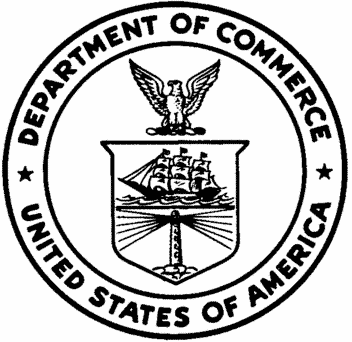
\includegraphics[alt={},width=2cm]{support_files/us_doc_logo.png}\newline % empty curly brackets without alt text is suitable for this logo because it's purely decorative/an "artifact"
  U.S. Department of Commerce\newline
  National Oceanic and Atmospheric Administration\newline
  National Marine Fisheries Service\newline
  Northwest Fisheries Science Center\newline

  \end{minipage}
  \restoregeometry
  \end{titlepage}

\renewcommand*\contentsname{Table of contents}
{
\hypersetup{linkcolor=}
\setcounter{tocdepth}{3}
\tableofcontents
}

\pagenumbering{roman}
\setcounter{page}{1}

\renewcommand{\thetable}{\roman{table}}
\renewcommand{\thefigure}{\roman{figure}}

\newpage{}

Please cite this publication as:

Johnston, M., Rosemond, R. C., Perl, E., Whitman, A., Barros, M.,
Champagnat, J., Schamp, A., Schiano, S., and Prior Caltabellotta, F.
(2025) Status of Yelloweye rockfish off the U.S. West Coast in 2025.
Pacific Fishery Management Council. {[}XX{]} p.

\newpage{}

\pagenumbering{roman}
\setcounter{page}{1}

\renewcommand{\thetable}{\roman{table}}
\renewcommand{\thefigure}{\roman{figure}}

\section*{Disclaimer}\label{disclaimer}
\addcontentsline{toc}{section}{Disclaimer}

These materials do not constitute a formal publication and are for
information only. They are in a pre-review, pre-decisional state and
should not be formally cited or reproduced. They are to be considered
provisional and do not represent any determination or policy of NOAA or
the Department of Commerce.

\newpage{}

\begin{verbatim}
$SS_version
[1] "3.30.23.2;_safe;_compile_date:_Apr 17 2025;_Stock_Synthesis_by_Richard_Methot_(NOAA)_using_ADMB_13.2"

$SS_versionshort
[1] "3.30"

$SS_versionNumeric
[1] 3.3

$StartTime
[1] "StartTime: Wed May 14 00:13:02 2025"

$RunTime
[1] "0 hours, 22 minutes, 34 seconds."

$Files_used
[1] "Data_File: yelloweye_data.ss Control_File: yelloweye_control.ss"

$log_det_hessian
[1] 351.896

$Final_phase
[1] 8

$N_iterations
[1] 1392

$Nwarnings
[1] 7

$warnings
[1] "Note 1 Information: Max data length bin: 74  < max pop len bins: 88; so will accumulate larger pop len bins"                                               
[2] "Note 2 Suggestion:  recr_dist_method 3 is simpler and takes 1 parm for each settlement"                                                                    
[3] "Warning 1 : At least one block pattern ends in endyr. Check the output parameter value time series to see if the values in forecast years are as intended."
[4] "Warning 2 : Minimum pop size bin:_8; is > L at Amin for sex: 1; Gpat: 1; L= 1.47471"                                                                       
[5] "Warning 3 : Final gradient: 0.000865898 is larger than final_conv: 0.0001"                                                                                 
[6] "Note 3 Information:  N parameters that are on or within 1% of min-max bound: 1; check results, variance may be suspect"                                    
[7] " 3 warnings  and 3 notes "                                                                                                                                 

$likelihoods_used
                                            values lambdas
TOTAL                                7907.94000000      NA
Equil_catch                             0.00000000      NA
Survey                                  1.06399000      NA
Length_comp                          1384.50000000      NA
Age_comp                             6507.96000000      NA
Recruitment                            14.10160000    1.00
InitEQ_Regime                           0.00000000    1.00
Forecast_Recruitment                    0.00000000    1.00
Parm_priors                             0.00000000    1.00
Parm_softbounds                         0.00889951      NA
Parm_devs                               0.00000000    1.00
F_Ballpark                              0.30867200    1.00
F_Ballpark(info_only)_1999_estF_tgtF    0.10888800    0.09
Crash_Pen                               0.00000000    1.00

$likelihoods_laplace
                                      values lambdas
NoBias_corr_Recruitment(info_only)  -57.4556       1
Laplace_obj_fun(info_only)         7836.3900      NA

$likelihoods_by_fleet
              Label        ALL 1_CA_TWL 2_CA_NONTWL  3_CA_REC 4_ORWA_TWL
212 Init_equ_lambda         NA    1.000      1.0000   1.00000     1.0000
213   Init_equ_like    0.00000    0.000      0.0000   0.00000     0.0000
214     Surv_lambda         NA    0.000      0.0000   1.00000     0.0000
215       Surv_like    1.06399    0.000      0.0000  -4.40504     0.0000
216      Surv_N_use         NA    0.000      0.0000  15.00000     0.0000
217     Surv_N_skip         NA    0.000      0.0000   0.00000     0.0000
218   Length_lambda         NA    1.000      1.0000   1.00000     1.0000
219     Length_like 1384.50000  139.081     92.5693 264.93000    82.3613
220    Length_N_use         NA   38.000     44.0000  42.00000    29.0000
221   Length_N_skip         NA    0.000      0.0000   0.00000     0.0000
222      Age_lambda         NA    0.000      1.0000   1.00000     1.0000
223        Age_like 6507.96000    0.000    126.1870 334.84000  1602.3000
224       Age_N_use         NA    0.000     42.0000 102.00000   353.0000
225      Age_N_skip         NA    0.000     10.0000  16.00000    23.0000
    5_ORWA_NONTWL  6_OR_REC  7_WA_REC 8_CACPFV 9_OR_RECOB 10_TRI_ORWA
212        1.0000    1.0000   1.00000   1.0000     1.0000     1.00000
213        0.0000    0.0000   0.00000   0.0000     0.0000     0.00000
214        0.0000    1.0000   1.00000   1.0000     1.0000     1.00000
215        0.0000   25.9712  -4.72162  -6.9722    -4.5689    -1.28706
216        0.0000   36.0000  20.00000  11.0000    17.0000     9.00000
217        0.0000    0.0000   0.00000   0.0000     0.0000     0.00000
218        1.0000    1.0000   1.00000   1.0000     1.0000     1.00000
219       88.6431  180.1390 118.40900 163.2280   106.4650    26.64520
220       31.0000   43.0000  26.00000  32.0000    20.0000     7.00000
221        0.0000    0.0000   0.00000   0.0000     0.0000     0.00000
222        1.0000    1.0000   1.00000   0.0000     0.0000     0.00000
223      430.8030 1007.1400 807.99300   0.0000     0.0000     0.00000
224      266.0000  195.0000 177.00000   0.0000     0.0000     0.00000
225       23.0000   16.0000  20.00000   0.0000     0.0000     0.00000
    11_NWFSC_ORWA 12_IPHC_ORWA
212       1.00000      1.00000
213       0.00000      0.00000
214       1.00000      1.00000
215      -5.69629      2.74385
216      21.00000     21.00000
217       0.00000      0.00000
218       1.00000      1.00000
219      67.52970     54.50320
220      21.00000     21.00000
221       0.00000      0.00000
222       1.00000      1.00000
223    1370.05000    828.64700
224     382.00000    531.00000
225      21.00000     36.00000

$N_estimated_parameters
[1] 188

$table_of_phases

-99 -50  -6  -5  -4  -3  -2  -1   1   2   3   4   5   6   7   8 
  1  10   2  31  11   1   1   9   2   2   3  20  10   2 136  13 

$estimated_non_dev_parameters
                                           Value Phase   Min   Max       Init
L_at_Amin_Fem_GP_1                     1.4747100     2  0.01  35.0  1.4747100
L_at_Amax_Fem_GP_1                    61.3823000     2 40.00 120.0 61.3823000
VonBert_K_Fem_GP_1                     0.0759819     1  0.01   0.2  0.0759819
CV_young_Fem_GP_1                      0.1482920     3  0.01   0.5  0.1482920
CV_old_Fem_GP_1                        0.0642259     7  0.01   0.5  0.0642259
RecrDist_Area_2                        0.4602840     3 -4.00   4.0  0.4602840
SR_LN(R0)                              5.4351500     3  3.00  15.0  5.4351500
Q_extraSD_3_CA_REC(3)                  0.1324150     5  0.00   5.0  0.1324150
Q_extraSD_6_OR_REC(6)                  1.0445400     5  0.00   5.0  1.0445400
Q_extraSD_7_WA_REC(7)                  0.4063890     5  0.00   5.0  0.4063890
Q_extraSD_8_CACPFV(8)                  0.0794343     5  0.00   5.0  0.0794342
Q_extraSD_9_OR_RECOB(9)                0.1663750     5  0.00   5.0  0.1663750
Q_extraSD_10_TRI_ORWA(10)              0.1299870     5  0.00   5.0  0.1299870
Q_extraSD_12_IPHC_ORWA(12)             0.5510650     5  0.00   5.0  0.5510650
LnQ_base_6_OR_REC(6)_BLK2add_2005     -0.5979600     1 -4.00   4.0 -0.5981050
Size_DblN_peak_1_CA_TWL(1)            43.9522000     4 20.00  60.0 43.9522000
Size_DblN_ascend_se_1_CA_TWL(1)        5.1261900     4 -1.00   9.0  5.1261900
Size_DblN_descend_se_1_CA_TWL(1)      18.2819000     5 -1.00  30.0 18.2818000
Size_DblN_peak_2_CA_NONTWL(2)         44.4293000     4 20.00  60.0 44.4293000
Size_DblN_ascend_se_2_CA_NONTWL(2)     5.1833000     4 -1.00   9.0  5.1833000
Size_DblN_descend_se_2_CA_NONTWL(2)   17.3737000     5 -1.00  30.0 17.3738000
Size_DblN_peak_3_CA_REC(3)            41.8052000     4 20.00  60.0 41.8052000
Size_DblN_ascend_se_3_CA_REC(3)        5.2204900     4 -1.00   9.0  5.2204900
Size_DblN_peak_4_ORWA_TWL(4)          41.8841000     4 20.00  60.0 41.8842000
Size_DblN_ascend_se_4_ORWA_TWL(4)      5.4868800     4 -1.00   9.0  5.4868800
Size_DblN_descend_se_4_ORWA_TWL(4)    18.1355000     5 -1.00  30.0 18.1352000
Size_DblN_peak_5_ORWA_NONTWL(5)       50.6925000     4 20.00  60.0 50.6925000
Size_DblN_ascend_se_5_ORWA_NONTWL(5)   5.4237700     4 -1.00   9.0  5.4237700
Size_DblN_peak_6_OR_REC(6)            36.8398000     4 20.00  60.0 36.8398000
Size_DblN_ascend_se_6_OR_REC(6)        4.1468000     4 -1.00   9.0  4.1468000
Size_DblN_peak_7_WA_REC(7)            42.7236000     6 20.00  60.0 42.7236000
Size_DblN_ascend_se_7_WA_REC(7)        4.3105600     6 -1.00   9.0  4.3105600
Size_DblN_peak_9_OR_RECOB(9)          35.0963000     4 20.00  60.0 35.0963000
Size_DblN_ascend_se_9_OR_RECOB(9)      4.6044200     4 -1.00   9.0  4.6044200
Size_DblN_peak_10_TRI_ORWA(10)        79.9714000     4 20.00  80.0 79.9714000
Size_DblN_ascend_se_10_TRI_ORWA(10)    7.0829600     4 -1.00   9.0  7.0829600
Size_DblN_peak_11_NWFSC_ORWA(11)      48.5565000     4 20.00  60.0 48.5565000
Size_DblN_ascend_se_11_NWFSC_ORWA(11)  6.2146900     4 -1.00   9.0  6.2146900
Size_DblN_peak_12_IPHC_ORWA(12)       53.9679000     4 20.00  60.0 53.9679000
Size_DblN_ascend_se_12_IPHC_ORWA(12)   4.1372900     4 -1.00   9.0  4.1372900
                                      Status    Parm_StDev         Gradient
L_at_Amin_Fem_GP_1                        OK    0.58067900 -0.0000258040000
L_at_Amax_Fem_GP_1                        OK    0.22502600 -0.0004515410000
VonBert_K_Fem_GP_1                        OK    0.00132433 -0.0002933460000
CV_young_Fem_GP_1                         OK    0.00679028 -0.0000216916000
CV_old_Fem_GP_1                           OK    0.00194060 -0.0000152147000
RecrDist_Area_2                           OK    0.02239730  0.0002962430000
SR_LN(R0)                                 OK    0.06210570 -0.0008658900000
Q_extraSD_3_CA_REC(3)                     OK    0.08083150  0.0000053765900
Q_extraSD_6_OR_REC(6)                     OK    0.14915400 -0.0000020286800
Q_extraSD_7_WA_REC(7)                     OK    0.08029780  0.0000046156500
Q_extraSD_8_CACPFV(8)                     OK    0.07113640  0.0000116549000
Q_extraSD_9_OR_RECOB(9)                   OK    0.07950520  0.0000031767800
Q_extraSD_10_TRI_ORWA(10)                 OK    0.11924100  0.0000013354500
Q_extraSD_12_IPHC_ORWA(12)                OK    0.10640000  0.0000026669400
LnQ_base_6_OR_REC(6)_BLK2add_2005         OK 7821.22000000 -0.0000000593718
Size_DblN_peak_1_CA_TWL(1)                OK    3.29106000 -0.0000230546000
Size_DblN_ascend_se_1_CA_TWL(1)           OK    0.40203200  0.0000327405000
Size_DblN_descend_se_1_CA_TWL(1)          OK  151.72100000  0.0000001532420
Size_DblN_peak_2_CA_NONTWL(2)             OK    2.48446000 -0.0000142103000
Size_DblN_ascend_se_2_CA_NONTWL(2)        OK    0.28386700  0.0000265114000
Size_DblN_descend_se_2_CA_NONTWL(2)       OK  171.54800000  0.0000006927240
Size_DblN_peak_3_CA_REC(3)                OK    1.36029000 -0.0000459692000
Size_DblN_ascend_se_3_CA_REC(3)           OK    0.14357200  0.0000557261000
Size_DblN_peak_4_ORWA_TWL(4)              OK    2.98270000 -0.0000055137200
Size_DblN_ascend_se_4_ORWA_TWL(4)         OK    0.33837600  0.0000161098000
Size_DblN_descend_se_4_ORWA_TWL(4)        OK  154.57500000  0.0000002412800
Size_DblN_peak_5_ORWA_NONTWL(5)           OK    1.47962000 -0.0000057693700
Size_DblN_ascend_se_5_ORWA_NONTWL(5)      OK    0.14822000 -0.0000042702900
Size_DblN_peak_6_OR_REC(6)                OK    1.30948000 -0.0000217942000
Size_DblN_ascend_se_6_OR_REC(6)           OK    0.28575300  0.0000260836000
Size_DblN_peak_7_WA_REC(7)                OK    2.74742000 -0.0000198470000
Size_DblN_ascend_se_7_WA_REC(7)           OK    0.51791300  0.0000327997000
Size_DblN_peak_9_OR_RECOB(9)              OK    1.61130000 -0.0000187959000
Size_DblN_ascend_se_9_OR_RECOB(9)         OK    0.28983500  0.0000210250000
Size_DblN_peak_10_TRI_ORWA(10)            HI    0.90522700  0.0000018156800
Size_DblN_ascend_se_10_TRI_ORWA(10)       OK    0.26644100 -0.0000060550100
Size_DblN_peak_11_NWFSC_ORWA(11)          OK    5.44640000 -0.0000071116100
Size_DblN_ascend_se_11_NWFSC_ORWA(11)     OK    0.37941400  0.0000059259400
Size_DblN_peak_12_IPHC_ORWA(12)           OK    1.22122000 -0.0000106101000
Size_DblN_ascend_se_12_IPHC_ORWA(12)      OK    0.23465000  0.0000251788000
                                       Pr_type Prior Pr_SD Pr_Like Afterbound
L_at_Amin_Fem_GP_1                    No_prior    NA    NA      NA         OK
L_at_Amax_Fem_GP_1                    No_prior    NA    NA      NA         OK
VonBert_K_Fem_GP_1                    No_prior    NA    NA      NA         OK
CV_young_Fem_GP_1                     No_prior    NA    NA      NA         OK
CV_old_Fem_GP_1                       No_prior    NA    NA      NA         OK
RecrDist_Area_2                       No_prior    NA    NA      NA         OK
SR_LN(R0)                             No_prior    NA    NA      NA         OK
Q_extraSD_3_CA_REC(3)                 No_prior    NA    NA      NA         OK
Q_extraSD_6_OR_REC(6)                 No_prior    NA    NA      NA         OK
Q_extraSD_7_WA_REC(7)                 No_prior    NA    NA      NA         OK
Q_extraSD_8_CACPFV(8)                 No_prior    NA    NA      NA         OK
Q_extraSD_9_OR_RECOB(9)               No_prior    NA    NA      NA         OK
Q_extraSD_10_TRI_ORWA(10)             No_prior    NA    NA      NA         OK
Q_extraSD_12_IPHC_ORWA(12)            No_prior    NA    NA      NA         OK
LnQ_base_6_OR_REC(6)_BLK2add_2005     No_prior    NA    NA      NA         OK
Size_DblN_peak_1_CA_TWL(1)            No_prior    NA    NA      NA         OK
Size_DblN_ascend_se_1_CA_TWL(1)       No_prior    NA    NA      NA         OK
Size_DblN_descend_se_1_CA_TWL(1)      No_prior    NA    NA      NA         OK
Size_DblN_peak_2_CA_NONTWL(2)         No_prior    NA    NA      NA         OK
Size_DblN_ascend_se_2_CA_NONTWL(2)    No_prior    NA    NA      NA         OK
Size_DblN_descend_se_2_CA_NONTWL(2)   No_prior    NA    NA      NA         OK
Size_DblN_peak_3_CA_REC(3)            No_prior    NA    NA      NA         OK
Size_DblN_ascend_se_3_CA_REC(3)       No_prior    NA    NA      NA         OK
Size_DblN_peak_4_ORWA_TWL(4)          No_prior    NA    NA      NA         OK
Size_DblN_ascend_se_4_ORWA_TWL(4)     No_prior    NA    NA      NA         OK
Size_DblN_descend_se_4_ORWA_TWL(4)    No_prior    NA    NA      NA         OK
Size_DblN_peak_5_ORWA_NONTWL(5)       No_prior    NA    NA      NA         OK
Size_DblN_ascend_se_5_ORWA_NONTWL(5)  No_prior    NA    NA      NA         OK
Size_DblN_peak_6_OR_REC(6)            No_prior    NA    NA      NA         OK
Size_DblN_ascend_se_6_OR_REC(6)       No_prior    NA    NA      NA         OK
Size_DblN_peak_7_WA_REC(7)            No_prior    NA    NA      NA         OK
Size_DblN_ascend_se_7_WA_REC(7)       No_prior    NA    NA      NA         OK
Size_DblN_peak_9_OR_RECOB(9)          No_prior    NA    NA      NA         OK
Size_DblN_ascend_se_9_OR_RECOB(9)     No_prior    NA    NA      NA         OK
Size_DblN_peak_10_TRI_ORWA(10)        No_prior    NA    NA      NA         OK
Size_DblN_ascend_se_10_TRI_ORWA(10)   No_prior    NA    NA      NA         OK
Size_DblN_peak_11_NWFSC_ORWA(11)      No_prior    NA    NA      NA         OK
Size_DblN_ascend_se_11_NWFSC_ORWA(11) No_prior    NA    NA      NA         OK
Size_DblN_peak_12_IPHC_ORWA(12)       No_prior    NA    NA      NA         OK
Size_DblN_ascend_se_12_IPHC_ORWA(12)  No_prior    NA    NA      NA         OK

$maximum_gradient_component
[1] 0.000865898

$parameters_with_highest_gradients
                                     Value     Gradient
SR_LN(R0)                        5.4351500 -8.65890e-04
L_at_Amax_Fem_GP_1              61.3823000 -4.51541e-04
RecrDist_Area_2                  0.4602840  2.96243e-04
VonBert_K_Fem_GP_1               0.0759819 -2.93346e-04
Size_DblN_ascend_se_3_CA_REC(3)  5.2204900  5.57261e-05

$Length_Comp_Fit_Summary
     Data_type Fleet Recommend_var_adj #  N Npos min_Nsamp max_Nsamp
5980         4     1          0.507141 # 38   38  0.593431  16.13210
5981         4     2          0.408988 # 44   44  0.653378  50.21250
5982         4     3          0.574349 # 42   42  2.838190  82.99970
5983         4     4          0.582423 # 29   29  1.266420  33.16560
5984         4     5          0.436315 # 31   31  0.922722 100.75400
5985         4     6          0.224649 # 43   43  0.820298 135.93700
5986         4     7          0.504250 # 26   26  1.138000  33.08200
5987         4     8          0.336157 # 32   32  1.887900  63.87120
5988         4     9          0.573264 # 20   20  1.226630  24.35200
5989         4    10          1.294940 #  7    7  1.680730   7.68335
5990         4    11          2.052860 # 21   21  4.191720  13.39460
5991         4    12          2.383500 # 21   21 14.212700  52.87600
     mean_Nsamp_in mean_Nsamp_adj mean_Nsamp_DM err_method err_index
5980       9.93300        5.17974            NA          0        NA
5981      34.92250       10.02530            NA          0        NA
5982      45.84090       24.18310            NA          0        NA
5983      37.23070        9.49450            NA          0        NA
5984      79.26010       28.65790            NA          0        NA
5985      52.47780       18.91360            NA          0        NA
5986       7.25315        7.25315            NA          0        NA
5987      37.58630       20.78480            NA          0        NA
5988      25.59210       13.79260            NA          0        NA
5989      11.24710        5.09527            NA          0        NA
5990      16.07050        8.44147            NA          0        NA
5991      28.71880       25.47880            NA          0        NA
            par1 val1 par2 val2 mean_effN  HarMean Curr_Var_Adj    Fleet_name
5980 multinomial   NA   NA   NA   14.8142  5.03743     0.521468      1_CA_TWL
5981 multinomial   NA   NA   NA   81.5419 14.28290     0.287073   2_CA_NONTWL
5982 multinomial   NA   NA   NA   49.9643 26.32870     0.527545      3_CA_REC
5983 multinomial   NA   NA   NA   59.2346 21.68400     0.255018    4_ORWA_TWL
5984 multinomial   NA   NA   NA  124.5060 34.58240     0.361568 5_ORWA_NONTWL
5985 multinomial   NA   NA   NA   52.8324 11.78910     0.360412      6_OR_REC
5986 multinomial   NA   NA   NA   33.2542  3.65740     1.000000      7_WA_REC
5987 multinomial   NA   NA   NA   54.7718 12.63490     0.552988      8_CACPFV
5988 multinomial   NA   NA   NA   42.7617 14.67110     0.538939    9_OR_RECOB
5989 multinomial   NA   NA   NA   20.3055 14.56440     0.453028   10_TRI_ORWA
5990 multinomial   NA   NA   NA   38.0351 32.99050     0.525278 11_NWFSC_ORWA
5991 multinomial   NA   NA   NA   97.2455 68.45110     0.887182  12_IPHC_ORWA

$Age_Comp_Fit_Summary
     Data_type Fleet Recommend_var_adj # Nsamp_adj Npos min_Nsamp max_Nsamp
8211         5     2          0.972139 #        52   42  1.000000    3.0000
8212         5     3          0.884301 #       118  102  1.000000    6.0000
8213         5     4          0.540419 #       376  353  1.000000   24.0000
8214         5     5          0.290144 #       289  266  0.220948   15.0245
8215         5     6          0.556567 #       211  195  1.000000   16.0000
8216         5     7          0.544856 #       197  177  1.000000   17.0000
8217         5    11          0.760806 #       403  382  1.000000   12.0000
8218         5    12          0.235905 #       567  531  0.086445   10.0276
     mean_Nsamp_in mean_Nsamp_adj mean_Nsamp_DM err_method err_index
8211       1.38095        1.38095            NA          0        NA
8212       1.50000        1.50000            NA          0        NA
8213       4.20963        4.20963            NA          0        NA
8214       8.85714        1.95697            NA          0        NA
8215       4.09231        4.09231            NA          0        NA
8216       3.63277        3.63277            NA          0        NA
8217       2.27749        2.27749            NA          0        NA
8218      15.98310        1.38165            NA          0        NA
            par1 val1 par2 val2 mean_effN HarMean Curr_Var_Adj    Fleet_name
8211 multinomial   NA   NA   NA   1.65003 1.34248     1.000000   2_CA_NONTWL
8212 multinomial   NA   NA   NA   1.94201 1.32645     1.000000      3_CA_REC
8213 multinomial   NA   NA   NA   4.68598 2.27497     1.000000    4_ORWA_TWL
8214 multinomial   NA   NA   NA   8.44721 2.56985     0.220948 5_ORWA_NONTWL
8215 multinomial   NA   NA   NA   4.73032 2.27764     1.000000      6_OR_REC
8216 multinomial   NA   NA   NA   4.49136 1.97934     1.000000      7_WA_REC
8217 multinomial   NA   NA   NA   3.06105 1.73273     1.000000 11_NWFSC_ORWA
8218 multinomial   NA   NA   NA  10.09310 3.77048     0.086445  12_IPHC_ORWA

$SBzero
[1] 564.8515

$current_depletion
[1] 0.3778621

$SPRratioLabel
[1] "(1-SPR)/(1-SPR_50%)"

$sigma_R_in
[1] 0.5

$sigma_R_info
           period N_devs SD_of_devs Var_of_devs   mean_SE mean_SEsquared
1            Main     44  0.5718538   0.3270168 0.3497106      0.1272598
2      Early+Main    135  0.3669449   0.1346486 0.4319109      0.1927868
3 Early+Main+Late    136  0.3655846   0.1336521 0.4324116      0.1932075
  sqrt_sum_of_components SD_of_devs_over_sigma_R sqrt_sum_over_sigma_R
1              0.6740004               1.1437077              1.348001
2              0.5722197               0.7338898              1.144439
3              0.5717163               0.7311691              1.143433
  alternative_sigma_R
1   0.674000435695887
2   0.572219681284994
3   0.571716330143147

$rmse_table
    ERA  N     RMSE RMSE_over_sigmaR mean_BiasAdj
1  main 44 0.565318         1.278340     0.482081
2 early 91 0.209602         0.175732     0.115969

$RecDev_method
[1] 1
\end{verbatim}

\newpage{}

\setlength{\parskip}{5mm plus1mm minus1mm}
\pagenumbering{arabic}
\setcounter{page}{1}
\setcounter{section}{0}
\renewcommand{\thefigure}{\arabic{figure}}
\renewcommand{\thetable}{\arabic{table}}
\setcounter{table}{0}
\setcounter{figure}{0}

\section{Introduction}\label{introduction}

Yelloweye Rockfish (\emph{Sebastes ruberrimus}) are found from the Gulf
of Alaska to northern Baja California in Mexico across the northeastern
Pacific Ocean Love, Yoklavich, and Thorsteinson (2002). Their core
distribution is from southeast Alaska to central California on the west
coast of the United States (Love, Yoklavich, and Thorsteinson 2002).
Yelloweye Rockfish in Puget Sound are considered isolated from the
coastal waters population (\textbf{stewart\_status\_2009?}) and have
been listed as threatened under the Endangered Species Act since 2010
(Drake J. S. and Williams 2010).

Yelloweye Rockfish are strongly associated with rocky bottom habtiat,
particularly areas of high relief (Love, Yoklavich, and Thorsteinson
2002), and adults are considered to be solitary and sedentary after
settlement DeMott (1983). However, new tagging studies suggest that
adult Yelloweye Rockfish exhibit larger scale movement patterns more
commonly than preivously considered Rasmuson LK and TK (2025).

There has been little advancement on information pertaining to the stock
structure of Yelloweye Rockfish since the previous benchmark assessment.
As noted in Gertseva and Cope (2017), there is evidence of genetic
diferences between Canadian waters (Strait of Georgia) and West coast
coastal populations of Yelloweye Rockfish but no evidence across coastal
populations (Siegle and Yamanaka 2013). Gao and Wallace (2010) found
that there was complete mixing of offspring from Oregon and Washington
waters using otolith isotope analyses, indicating a single spawning
stock in this portion of the Yelloweye Rockfish stock. Given the general
perception of the sedentary nature of Yelloweye Rockfish adults and the
moderate amount of mixing that occurs during the pelagic larval stage,
the previous Yelloweye Rockfish assessment modeled the West coast
population as a two-area assessment (California and a combined
Oregon-Washington) with a common recruitment relationship (Gertseva and
Cope 2017). This update assessment maintains this basic structure.

Map of scope of assessment - not needed for update

\subsection{Life History}\label{life-history}

This section is not required for an update assessment; please refer to
the most recent full assessment (Gertseva and Cope 2017) for additional
information.

\subsection{Ecosystem considerations}\label{ecosystem-considerations}

This section is not required for an update assessment; please refer to
the most recent full assessment (Gertseva and Cope 2017) for additional
information.

\subsection{Fishery description}\label{fishery-description}

This section is not required for an update assessment; please refer to
the most recent full assessment (Gertseva and Cope 2017) for additional
information.

\subsection{Management History}\label{management-history}

This section is not required for an update assessment; please refer to
the most recent full assessment (Gertseva and Cope 2017) for additional
information.

\subsection{Management performance}\label{management-performance}

Yelloweye Rockfish removals have been substantially reduced since its
designation as overfished in 2002 through a variety of managment
measures that eliminated retention in recreational fisheries, limited
commercial retention, created broad spatial closures and implemented new
gear restrictions that reduced trawling in rocky habitats. Many of these
restrictions remain in effect, though as Yelloweye Rockfish stock has
begun to rebuild, some managment measures have been modified or removed
in recent years. These include some additional allocations to
recreational fisheries that remain constrained by Yelloweye Rockfish
estimated discard mortality, the recent removal of the Yelloweye
Rockfish Conservation Areas (RCA) for the trawl sector off of California
and Oregon, and eliminating some gear restrictions in the RCAs for the
non-trawl sector.

Recent trends in total catch relative to managment guidelines is
available in (Table \ref{tbl-yelloweye_management}) and shows that total
catch of Yelloweye Rockfish has remained below both the OFLs and ACLs in
each year since the previous assessment. Catch in Table
\ref{tbl-yelloweye_management} combines the two areas in this model as
catch limits for Yelloweye Rockfish are managed as a single coastwide
unit and includes both landings and estimated discard mortality. As in
the previous assessment, total catches for each fleet in this update
include both landings and estimated dead discard mortality.

\subsection{Fisheries off Canada and
Alaska}\label{fisheries-off-canada-and-alaska}

This section is not required for an update assessment; please refer to
the most recent full assessment (Gertseva and Cope 2017) for additional
information.

\newpage{}

\section{Data}\label{data}

A summary of available data by type and fleet used in the yelloweye
rockfish assessment is available in Figure~\ref{fig-data}. Data that
have changed from the previous assessment are summarized below. No new
data sources were considered in this update assessment.

Removals: - Post-2016 landings and discards were updated for all three
states for the commercial and recreational fleets. - A new Oregon
historical recreational catch reconstruction was incorporated, which
covered 1979 - 2000. - A new Washington historical recreational catch
reconstruction was provided by WDFW and included changes to data from
1990-2016.

Composition Data: - Length and age composition data were updated from
2017 - 2024 for all states for the commercial and recreational fleets. -
Length and age composition data were also updated for two of the
fishery-independent surveys, including the NWFSC Bottom Trawl survey and
the IPHC Longline survey. - Some length and age composition data from
the 2017 assessment had minor errors in how sample numbers were
calculated, ageing error assignment, and doubled age samples and thus
needed to be fixed. See Section~\ref{sec-fd_comps} below.

Indices of Abundance: -Indices that were updated with more recent data
and/or updated methodology include: -Oregon Onboard Observer (2001 -
2024) -Oregon ORBS Dockside (release only) (2004-2024) -NWFSC Bottom
Trawl Survey -IPHC Longline Survey

Biological Data: - Length-weight relationship parameters were updated to
include all the recent (2017 - 2024) fishery-independent data. - Ageing
error matrices were unchanged but some Oregon recreation ages were
assigned the wrong ageing error and were corrected based on ODFW
recommendations.

\subsection{Fishery-Dependent Data}\label{fishery-dependent-data}

Updated fishery-dependent data, including removals, length and age
compositions, and indices of abundance, are detailed below.

\subsubsection{Landings}\label{landings}

A summary of total removals are provided in
\textbf{Table~\ref{tbl-all_removals}} and Figure~\ref{fig-catch}.

Recent commercial landings (2017-2024) were obtained from
\href{www.pacfin.psmfc.org}{PacFIN} for California, Oregon and
Washington, and as with the previous assessment, for the period from
2016 through 2023, updated West Coast Groundfish Observer Program
(WCGOP) discard estimates were added to PacFIN landings by calculating
the proportion of observed area-specific fleet WCGOP discards expanded
from the fleet-specific GEMM total recorded discards to obtain the total
catch of yelloweye rockfish within commercial fleets.

Bycatch for the At-Sea Pacific Hake fleet (ASHOP) was updated from 2017
through 2024 and included in the trawl fleets for California and
Oregon/Washington.

Recreational removals from \href{www.recfin.org}{RecFIN} were updated
for California, Oregon and Washington from 2017 - 2024. RecFIN removals
include an estimate of discard mortality and represent total estimated
removals. Updated historical recreational removals for Oregon from 1979
through 2000 were provided by Oregon Department of Fish and Wildlife
(ODFW,(Whitman 2024)). Updated historical recreational removals for
Washington (1967-1989) and Washington Department of Fish and Wildlife
(WDFW) Ocean Sampling Program (OSP) estimates (1990-2001) were provided
by WDFW (\textbf{Fabio/RecFin?} May pull). The historical recreational
removals for 1971, 1974, and 1979 were not available and were treated as
the average of the two preceding and two following years. Historical
data were filtered to marine catch areas 1-4. For OSP catch estimates,
data included marine catch areas 1-4, up to the Bonilla-Tatoosh line.
WDFW also provided updated catch estimates for 2002-2004, which did not
include discard mortality. To adjust for this, we multiplied the average
mortality rate from the following 5 years (2005-2009) by the total
discards to calculate total mortality for those years.

\subsubsection{Fishery-Dependent Length and Age
Compositions}\label{sec-fd_comps}

Updated length composition data for commercial catches (trawl and
non-trawl) were available from PacFIN (extracted April 4, 2025) and from
WCGOP for all three states. These include the years 2017 - 2024 for
PacFIN data and 2017 - 2023 for WCGOP data. Updated recreational length
composition data were available from RecFIN (extracted April 4, 2025)
for all three states, and include years 2017 - 2024. Additionally,
updated length compositions from the California On-Board CPFV Observer
Sampling Program and from the Ocean Recreational Fishery Survey (ORFS,
previously the Oregon onboard recreational observer program), both of
which measure fish discarded at sea, were also available up through 2024
on RecFIN.

New commercial age composition data was unavailable for California, but
was available for both Oregon and Washington for 2017 - 2024 from PacFIN
and WCGOP. New recreational age composition data was unavailable for
California and Oregon, but was available for Washington for 2017 - 2024
from RecFIN (extracted May 13, 2025). These data were collected in the
MRFSS and in the WDFW Ocean Sampling Program (OSP). There were also some
historical updates to Oregon and Washington recreational age data
provided by the state representatives.

In combining the new data with the 2017 assessment data, we applied some
general processes and fixed minor data entry mistakes found in the old
assessment data file. For length composition data, years with small
samples sizes (N = 1) were excluded. Sampling statistics (number of
samples and number of individual fish) for each fleet and year were used
to create length frequency distributions. There were no changes in how
commercial length sample numbers were calculated. However, all recent
recreational fleet length data were missing the total number of trips
information used to calculate the number of samples. Using data from the
2017 assessment, we built fleet-specific linear regressions to
approximate the relationship of samples to the number of fish. Then, we
applied that regression to the total number of fish for data between
2017 and 2024 to estimate the number of samples. A future benchmark
assessment should investigate how to get the number of sampled trips
from RecFIN to calculate the number of samples using the Stewart and
Hamel (2014) method.

We also found that conditional-age-at-length (CAAL) data from the 2017
assessment had all sample sizes and ages doubled, potentially from when
Yelloweye Rockfish was changed from a two-sex to single-sex model. To
fix the CAAL data so it accurately represented the number of fish in
each age class, we either rebuilt the entire fleet's CAAL dataframe
using the most recently pulled information from PacFIN and RecFIN, or
divided the number of samples and ages in each length bin by two.

How these problems were treated for each fleet specifically is detailed
below, including other minor data changes. Otherwise, length and age
composition data are unchanged from the previous assessment; please
refer to the most recent benchmark assessment (Gertseva and Cope 2017)
for additional information.

\paragraph{Fleet Specific Changes in the Compositional
Data}\label{fleet-specific-changes-in-the-compositional-data}

Fleet 2. California Non-Trawl - For ages, all the CAAL and
marginal-age-at-length (MAAL) data were recalculated using the most
recent age data pulled from PacFIN and WCGOP, to account for age
doubling in 2017.

Fleet 3. California Recreational - CAAL data for 1979-1984 were doubled,
so the number of samples and ages in each length bin was divided by two.
- CAAL data for 2009-2016 were doubled, but the raw data we received
from RecFin were correct, without doubled ages, so this time series was
replaced with newly pulled data. - We then re-built the MAAL data from
the updated CAAL for both time periods because there were errors in
previous data entry and sample number calculations.

Fleet 4. Oregon/Washington Trawl \& Fleet 5. Oregon/Washington Non-Trawl
- Both the OR/WA commercial fleets had all CAAL and MAAL data
recalculated using the most recent age data pulled from PacFIN and
WCGOP, to account for age doubling in 2017.

Fleet 6. Oregon Recreational - CAAL data was doubled so ages and sample
numbers from 1979 - 2017 were divided by two. - We included 2015 unsexed
ages. - We also reassigned the aging error for this fleet for the
correct years. The ODFW data representative confirmed that all fish from
1979-2002 were aged by WDFW (ageing error 1), and fish from 2009-2016
were aged by the NWFSC (ageing error 2). No new ages since 2016 were
provided. MAAL data were then recalculated from the updated CAAL so that
the ageing error labels and number of samples matched.

Fleet 7. Washington Recreational - All age data from 1998 to 2024 were
replaced with the most recent data provided in RecFIN, following the
recommendation of the WDFW representative, due to resolved ages based on
double readings in the age data. CAAL and MAAL were calculated using
this data.

\subsubsection{Indices of Abundance}\label{indices-of-abundance}

Two fishery-dependent indices of abundance were updated with new data
and up-to-date methodology. These are detailed below. Otherwise, indices
of abundances are unchanged from the previous assessment; please refer
to the most recent benchmark assessment (Gertseva and Cope 2017) for
additional information.

\paragraph{Oregon Onboard Observer CPUE, 2001 --
2024}\label{oregon-onboard-observer-cpue-2001-2024}

The Oregon Onboard Observer (now Ocean Recreational Fisheries Survey, or
ORFS) index was updated from the previous yelloweye rockfish assessment
and updated drift-level catch-per-unit-effort data was obtained from
ODFW through the end of 2024. The database contains information on catch
by species (number of retained and released fish), effort (angler
hours), sample depth, and bag limits and other relevant regulations
(Monk and Pearson 2013).

The unfiltered data set contained 18,410 drifts. Multiple standardized
filters are applied to remove outliers and data unsuitable for an index.
These filters are very similar to filters applied in 2017 and include
drifts without data needed for CPUE information, long drifts (below 95th
quantile), drifts in deeper waters (less than 64fm, 99th quantile),
drifts that were targeting primarily mid-water species, and drifts
outside of the legal fishing depth (with a five fm buffer).
Additionally, years with extreme low sample sizes (\textless50) were
excluded. Finally, drifts onboard charters from Port Orford were removed
due to small sample size. The final filtered dataset included 6,839
trips with a 6.1\% encounter rate for yelloweye rockfish.

Covariates evaluated included year, month, port, the open depths to
fishing (all depths or inside 20/30/40fm), and a five fm-binned depth of
drift covariate. This is in contrast to the 2017 index, which was only
able to evaluate a year covariate. The covariates listed above are
standard to evaluate for this index in other assessments. Negative
binomial models were fit using sdmTMB (version 0.6.0) to the drift-level
data (catch with a log offset for adjusted angler hours). A model
without the open fishing depths or month was selected as the best fit
model by AIC (\textbf{Table ``model selection''}). Acceptable
diagnostics for the model were achieved (Figure~\ref{fig-orfs_qqplot}).
The index of abundance in shown in Figure~\ref{fig-ORFS_index} and
\textbf{Table XXXX}. A comparison to the ORFS index used in the previous
assessment indicates that despite the change in modeling approach and
the covariates included, most years overlap between the two indices and
similar trends are observed ((\textbf{ORFS\_comp?})). The updated index
has reduced within-year variance and a lack of extreme swings in the
standardized index value (e.g.~2013).

\paragraph{Oregon ORBS Dockside (release only) CPUE,
2004-2024}\label{oregon-orbs-dockside-release-only-cpue-2004-2024}

The Ocean Recreational Boat Survey (ORBS) dockside index for Oregon was
updated for this assessment. CPUE, expressed in terms of fish per
angler-hour, was calculated by multiplying the number of anglers and the
total trip time, minus the boat type-specific travel time. The database
contains information on released fish by species (number of
angler-reported released fish), effort (angler hours), sample location
(port where data were collected), date, bag limits and other relevant
regulations, boat type (charter or private), and trip type (e.g., bottom
associated fish).

The unfiltered data set contained 504,128 trips from 2001 - 2024. Since
the previous yelloweye assessment, multiple data filters have been
standardized, which are very similar to the 2017 assessment, and are
applied to ORBS trip-level data to remove outliers and data unsuitable
for an index. For this index, the time period was restricted to years
when retention of yelloweye rockfish was prohibited, which began on
January 1, 2004. There were two differences in the filtering in this
updated index. One, the previous index began in 2005, which was
determined to be an error in the timing of the implementation of
prohibited status for yelloweye. Given that prohibition was in effect on
January 1, the year 2004 is included in this updated index. The second
difference in filtering is the elimination of the Stephens-MacCall
filter in the updated index. This filter has not been used for several
assessment cycles, based on a recommendation from NWFSC staff (pers.
comm. A. Whitman, ODFW). The final dataset included 133,039 trips
(\textbf{TABLE ``percent\_pos.csv''}) from 2004 -- 2024 with an overall
encounter rate of 7.4\%.

Covariates evaluated included year, month, port, the open depths to
fishing (all depths or inside 20/30/40 fm), and boat type. These are the
same covariates evaluated in the 2017 ORBS index, apart from the open
depths of the fishery. The final model in 2017 included boat type, port
and year. Negative binomial models were fit in sdmTMB (Version 0.6.0) to
the trip-level data (catch with a log offset for adjusted angler hours).
The final model selected includes year, month, port, boat type and open
fishery depths, which was the best fit model by AIC in this series
(\textbf{TABLE ``model\_selection.csv''}). Acceptable diagnostics for
the model were achieved (Figure~\ref{fig-orbs_qq}). The index of
abundance in shown in Figure~\ref{fig-ORBS_index} and \textbf{Table
XXXX}. ODFW no longer maintains the deltaGLM code that was used to
develop the 2017 index and so the index was updated to use the currently
accepted modeling approach for PFMC groundfish assessments (sdmTMB). To
bridge this change, the 2017 model index structure was applied to the
current dataset using sdmTMB and compared to the deltaGLM index used in
the 2017 assessment and the current recommended updated index in
Figure~\ref{fig-ORBS_comp}. There are some differences observed in 2005
-- 2009 between the deltaGLM index and the two sdmTMB indices; however,
this appears to be largely driven by the updated modeling approach.

\subsection{Fishery-Independent Data}\label{fishery-independent-data}

Two sources of fishery-independent data were updated. These include the
NWFSC West Coast Bottom Trawl Survey and the IPHC Longline survey.

\subsubsection{NWFSC West Coast Bottom Trawl Survey
(WCGBTS)}\label{nwfsc-west-coast-bottom-trawl-survey-wcgbts}

The WCGBTS survey methods are most recently described in detail in
Keller, Wallace, and Methot (2017). Geostatistical models of biomass
density were fit to survey data from the WCGBTS using \gls{tmb}
(Kristensen et al. 2016) via the \gls{sdmtmb} R package (Anderson et al.
2024) as configured within the \gls{indexwc} R package (Johnson et al.
2025). Code to reproduce the analysis is available
\href{https://github.com/pfmc-assessments/indexwc}{online}. These models
can account for latent spatial factors with a constant spatial Gaussian
random field and spatiotemporal deviations to evolve as a random walk
Guassian random field (Thorson et al. 2015). Delta-gamma and
delta-lognormal distributions were investigated. Results are only shown
for the model that led to the best model diagnostics, e.g., similar
distributions of theoretical normal quantiles and model quantiles
(Figure~\ref{fig-wcgbts_qq}), high precision, lack of extreme
predictions, and low \gls{aic}. Estimates of biomass from this best
model were predicted using a grid based on available survey locations.

The final model used a delta model with a lognormal distribution for the
catch-rate component. A logit-link was used for encounter probability
and a log-link for positive catch rates. The response variable was catch
(mt) with an offset of area (km\textsuperscript{2}) to account for
differences in effort. Fixed effects were estimated for each year and
pass. The index was estimated for the area north of \(42^{\circ}10'\)
(Oregon and Washington) to be consistent with the previous assessment.
The data were truncated to depths less than 325 m prior to modeling
given that there were zero positive encounters in depths deeper than 325
m. The prediction grid was also truncated to only include available
survey locations in depths between 55--325 m to limit extrapolating
beyond the data and edge effects. Spatial variation was included in the
encounter probability and the positive catch rate model. Spatial
variation was approximated using 200 knots, where more knots led to
non-estimable standard errors because the positive encounters are too
sparse to support the dense spatiotemporal structure. Anisotropy was not
estimated.

The biomass estimates produced for this assessment using sdmTMB are
comparable to the biomass estimates produced in the previous benchmark
assessment (Figure~\ref{fig-wcgbtsindexcomparison}). The index is
relatively flat with a peak in 2014, but variation is high throughout
the time series (Figure~\ref{fig-wcgbtsindex}).

\subsubsection{IPHC Setline Survey}\label{iphc-setline-survey}

The IPHC has conducted an annual longline survey for Pacific halibut off
the coast of Oregon and Washington (IPHC area ``2A'') since 1997 (no
surveys were performed in 1998 or 2000). Beginning in 1999, this has
been a fixed station design, with roughly 1,800 hooks deployed at each
of 84 locations. Before 1999, station locations were not fixed, and,
therefore, those years are not used in the index. Rockfish bycatch,
mainly yelloweye, was recorded during this survey, although values for
1999 and 2001 are estimates based on subsampling the first 20 hooks of
each 100-hook skate. The gear used to conduct this survey, while
designed specifically to efficiently sample Pacific halibut, is similar
to that used in some earlier line fisheries that targeted adult
yelloweye rockfish. Some variability in exact sampling location is
unavoidable, and leeway is given in the IPHC methods to center the set
on the target coordinates but to allow wind and currents to dictate the
actual direction in which the gear is deployed. This can result in
different habitats accessed at each fixed location among years. The
number of skates used can also differ from year to year; skates hauled
(i.e., 100 hooks/skate) are thus used as the unit of effort for all
years. This has been the standard effort used in past yelloweye rockfish
stock assessments.

New to this assessment is the consideration of eight additional survey
stations (1527 to 1534) conducted in a collaborative effort between IPHC
and WDFW from 2007-2009 then from 2013-2019 and 2021-2023. These
stations are arranged around IPHC station 1082 (one of the more notable
stations to encounter yelloweye rockfish). Only the summer months are
considered here to match the time of year sampled by the IPHC survey.
Survey sets at the WDFW stations used 3 skates with 100 hooks each for
most years, except for 2021 - 2023, where a total of 4 skates were used.
Like the IPHC survey, effort was standardized to 100 hooks/skate. These
stations were integrated into the IPHC stations when calculating the
index of abundance. The full survey used in this assessment combined all
stations in Oregon and Washington into a single index, fitting the area
of the stock, instead of using state-specific indices. Data were first
filtered to remove all depths with few or no encounters, and then we
excluded stations that rarely encountered yelloweye (averaging less than
one encounter a year). This left a total of 11 stations for analysis.
Both filtering levels increased the percentage of encounters from an
initial 11\% to 80\%.

A log-normal generalized linear model with a log link in the ``sdmTMB''
R package was used to standardize the CPUE. Model selection using the
Akaike Information Criteria for small samples (AICc) was conducted to
select which variables were included in the model. The final model
included year, station, and depth as explanatory variables. Diagnostic
tools to ensure the model fit was satisfactory included checking whether
the hessian matrix is positive definite, the presence of extreme
eigenvalues, and if the non-linear minimizer suggests convergence. These
diagnostics were conducted with the ``sanity( )'' function in the sdmTMB
package. The updated index is shown in Figure~\ref{fig-IPHC_index} and
compared to the index used in the 2017 index in
Figure~\ref{fig-IPHC_comparison}.

\subsubsection{Fishery-Independent Length and Age
Compositions}\label{fishery-independent-length-and-age-compositions}

Updated length and age composition data were available for the two
updated fishery-independent surveys. Compositional data from 2017
through 2024 were updated for NWFSC West Coast Groundfish Bottom Trawl
Survey were obtained using functions from the \textbf{\{nwfscSurvey\} R
package}. The IPHC survey data were provided by WDFW.

A summary of sampling efforts (number of hauls and number of individual
fish) in all surveys is provided in \textbf{Table X} and \textbf{Table
X}. Updated year-specific length frequency distributions generated for
each survey are shown in Figure~\ref{fig-NWFSC_lencomps} and
Figure~\ref{fig-IPHC_lencomps}, respectively. Updated year-specific CAAL
frequencies for each survey are shown in
Figure~\ref{fig-NWFSC_agecomps1} and Figure~\ref{fig-NWFSC_agecomps2}
for the WCGBTS and Figure~\ref{fig-IPHC_agecomps1} and
Figure~\ref{fig-IPHC_agecomps2}.

\subsection{Biological Parameters and
Data}\label{biological-parameters-and-data}

The approach to natural mortality, maturity and fecundity were unchanged
from the previous assessment (Gertseva and Cope 2017). Several
biological parameters used in the assessment were estimated outside the
model or obtained from literature. Their values were treated in the
model as fixed, and therefore uncertainty reported for the stock
assessment results does not include any uncertainty in these quantities
(however, some were investigated via sensitivity analyses described
later in this report). The parameters for the length-weight relationship
were updated to include the most recent data from 2017 - 2024. The
parameters derived from this analysis were as follows: ⍺ =
7.183309·10-6, and β = 3.244801 (Figure~\ref{fig-LWrel}). Aging error
matrices were unchanged but the designated matrix was corrected in some
years for Oregon recreational ages. All fish from 1979-2002 were aged by
WDFW (ageing error 1) and fish from 2009-2016 were aged by the NWFSC
(ageing error 2).

\newpage{}

\section{Assessment model}\label{assessment-model}

\subsection{History of modeling
approaches}\label{history-of-modeling-approaches}

This section is not required for an update assessment; please refer to
the most recent full assessment (Gertseva and Cope 2017) for additional
information.

\subsection{Responses to SSC Groundfish Subcommittee
requests}\label{responses-to-ssc-groundfish-subcommittee-requests}

To be completed after SSC GFSC review.

\subsection{Model Structure and
Assumptions}\label{model-structure-and-assumptions}

\subsubsection{Model Changes from the Last
Assessment}\label{sec-changes}

A list of changes that were made to the model compared to the previous
assessment (Gertseva and Cope 2017) are listed below.

ADW - what do we need to update after new WA catches incorporated into
base? Plus it seems like this section should go after the
platform/structure section, and we need to double check we're limiting
repetition with the model results section.

\begin{itemize}
\tightlist
\item
  Data

  \begin{itemize}
  \tightlist
  \item
    Detailed information on specific updates and changes to the data
    incldued in the model are included in Section 2 but are summarized
    below.
  \item
    The landings time series was corrected and updated through the end
    of 2024 for California, Oregon and Washington.
  \item
    Length and age compositions from all fishery removal and index
    fleets were updated through 2024.
  \item
    Some indices of abundance were updated with recent data, where
    available, and re-analyzed using more up-to-date methods. Two
    fishery-dependent indices from Oregon were updated, along with the
    fishery-independent indices, the WCBTS and the IPHC setline survey.
  \end{itemize}
\item
  Biology

  \begin{itemize}
  \tightlist
  \item
    No changes were made to the biological parameterization of the
    model; however, the length-weight relationship was updated to
    include the most recent data. -No changes were made to the aging
    error matrices estimated for the previous assessment; however, the
    designated matrix for several years of Oregon recreational ages were
    corrected.
  \end{itemize}
\item
  Recruitment

  \begin{itemize}
  \tightlist
  \item
    The bias adjustment ramp was updated to end with the last year of
    removals (2024) and begin to ramp to zero two years prior (2022)
  \end{itemize}
\item
  Software and Workflow

  \begin{itemize}
  \tightlist
  \item
    Update SS3 3.30.23.2 - As seen in Figures Figure~\ref{fig-ss3exe_1}
    and Figure~\ref{fig-ss3exe_2}, updating to the most recent version
    of the SS3 executable had no discernable impact on model results.
  \item
    Use most up-to-date R packages to process input and output files for
    the assessment, including \textbf{nwfscDiag, r4ss, and pacfintools}.
  \item
    Created a public github repository for Yelloweye Rockfish
    (``sebastes\_ruberrimus\_2025'') to provide a transparent and
    reproducible system for processing the data and creating the model
    and assessment document
  \end{itemize}
\end{itemize}

The iterative impact of the updated catch, composition and indices of
abundance on the model are shown in Figure~\ref{fig-newdata_1} and
Figure~\ref{fig-newdata_2}. Overall, there was little impact on the
model results when updating and extending the catch time series and when
updating the indices of abundance. However, the addition of the new
fishery length composition data decreased the spawning output
(Figure~\ref{fig-newdata_1}). When the new age composition data were
added, there was a slight increase in the scale of the population but
was overall very similar to the model with the new length composition
data (Figure~\ref{fig-newdata_3} and Figure~\ref{fig-newdata_4}). There
was very little impact on the model results when tuning the
compositional data and updating the bias adjustment ramp
(Figure~\ref{fig-newdata_5} and Figure~\ref{fig-newdata_6}). The impact
of the updated lenght-weight relationship is evalated as a sensitivity.

\subsubsection{Modeling Platform and
Structure}\label{modeling-platform-and-structure}

The assessment was updated to use the most recent version of Stock
Synthesis 3 (Version 3.30.23.2 - available
\href{https://github.com/nmfs-ost/ss3-source-code/releases/tag/v3.30.23.2}{online}).
Bridging between SS versions is discussed in Section
Section~\ref{sec-changes}.

Briefly, the Yelloweye Rockfish model is a coastwide, single-sex
two-area model. California is Area 1, and Oregon and Washington are
combined into Area 2, due to differences in potential exploitation rates
by area over time. Yelloweye Rockfish compositional data are primarily
reported as both sexes combined, and therefore, the previous assessment
used a single sex model to facilitate the use of all available data.
Growth is assumed to be the same in both areas, though future benchmark
assessments may want to re-evaluate this assumption if more
spatially-explicit data become available. The modeling period starts in
the first year of available catches from historical reconstructions
(1889) and the stock is assumed to be at an unfished equilibrium prior
to that time. No changes were made to the fleet structure of the model.
Fishery removals were divided among seven area- and sector-specific
fleets. Estimated discard mortality was added to landings and included
in the model as fleet-specific total removals. Length compositions for
discarded and retained fish were combined as well. Data weighting was
done using the Francis method (Francis 2011) but the McAllister-Ianelli
method was explored as a sensitivity. More detailed information on the
model structure and justification is available in Gertseva and Cope
(2017) and summarized in \textbf{?@tbl-table\_config}. (ADW - DO WE NEED
MORE DETAIL HERE?)

\subsubsection{Model Parameters}\label{model-parameters}

** ADW - update the code here to be sure we're getting the proper base
model. also do we need any more fig's from the base? **

The base model had r sum(mod\_out\$ parameters
\(Phase > 0) estimated parameters (tallied by type in @tbl-table_parcounts). A single-sex growth curve was estimated (@fig-growth). Natural mortality was fixed, as in the 2017 assessment. Unfished recruitment and the distribution of recruits between areas are estimated. Steepness of the stock-recruit relationship was kept fixed at 0.718, matching the 2017 assessment. Estimating steepness was evaluated as a sensitivity. Recruitment deviations during the "main" period (from r mod_in\)ctl\(MainRdevYrFirst to r mod_in\)ctl\$MainRdevYrLast)
were forced to sum to zero and the bias adjustment ranmp was updated
(Figure~\ref{fig-biasadj}).

Length, age, and age-at-length composition data weights were tuned using
the Francis method (Francis 2011, \textbf{?@tbl-table\_compweight}). All
selectivity was assumed to be length-based and used a double-normal
functional form. Selectivities for all fleets was estimated to be
asymptotic (Figure~\ref{fig-selex_allfleets}), though selectivity for
the California Onboard Observer CPUE was mirrored to the California
recreational fleet. Selectivity was constant through time. Dome-shaped
selectivity and various time blocks for specific fleets were explored in
Gertseva and Cope (2017) but not re-evaluted in this update assessment.

Aging error matrices were estimated outside the assessment model and
were unchanged from the previous assessment, with the exception of
correcting the designated error matrix in some years for the Oregon
recreational ages.

Additional standard error was estimated for all indices with the
exception of the WCBTS.

\subsubsection{Key Assumptions and Structural
Choices}\label{key-assumptions-and-structural-choices}

This section is not required for an update assessment; please refer to
the most recent full assessment (Gertseva and Cope 2017) for additional
information.

\subsection{Base Model Results}\label{base-model-results}

\subsubsection{Parameter Estimates}\label{parameter-estimates}

The list of the all the parameters used in the assessment model and
their values (either fixed or estimated) is provided in \textbf{Table
X}. The growth parameters estimated within the model are reasonable,
commensurate with inspection of the raw data and consistent with what we
know about the species. These parameters are relatively precisely
estimated, in terms of the asymptotic standard error estimates.
Figure~\ref{fig-growth} shows the estimated growth curve. Spawning
output-at-length is shown in Figure~\ref{fig-spoutlen}. Spawning output
in the assessment is expressed in millions of eggs.

Estimated stock-recruit function for the assessment model is shown in
\textbf{?@fig-SR\_curve}. Estimated recruitment deviations are shown
Figure~\ref{fig-recdevs_err}. Recruitment of yelloweye rockfish was
estimated to be quite variable over time, and the estimated
stock-recruit function predicts a relatively wide range of cohort sizes
over the observed range of spawning biomass. The model output
recruitment variance (RMSE = 0.48) is consistent with the fixed input
recruitment variance (R = 0.5).

Length-based selectivity curves estimated in the assessment are shown
for all fleets together in Figure~\ref{fig-selex_allfleets}. Estimated
selectivity curves for the fishing fleets indicate that the recreational
fleets access somewhat smaller fish than the commercial fisheries. This
pattern is most pronounced in Oregon, and also as expected, since recent
charter fishing selectivity has shifted shoreward where there is a
higher density of smaller fish. Addition of the charter vessel length
data did not appreciably change the estimate for the California
recreational selectivity pattern and so the selectivity for the two
series was not separated. All fleets for which curves were allowed to be
dome-shaped (commercial trawl and non-trawl fleets) were estimated to be
asymptotic. Estimated selectivity curves for the IPHC survey indicate a
selection of the largest yelloweye available, and select the least
amount of smaller yelloweye rockfish (Figure~\ref{fig-sel12}). The NWFSC
trawl survey selected far more smaller yelloweye among all surveys
(Figure~\ref{fig-sel11}). That the triennial survey selectivity was
shifted to the largest fish but also selected some very small fish is
likely an artifact of the very noisy composition data from that survey
(Figure~\ref{fig-sel10}).

\subsubsection{Fits to the Data}\label{fits-to-the-data}

Model fits to the fishery CPUE and survey indices are presented in
Figure~\ref{fig-indexfit3} through Figure~\ref{fig-indexfit12}. The base
model predicted a decreasing trend in the triennial survey between 1980
and 2004 (Figure~\ref{fig-indexfit10}) and a slightly increasing trend
for the NWFSC trawl survey between 2003 and 2024
(Figure~\ref{fig-indexfit11}). The model predicted a relatively flat
trend through the IPHC survey index despite the upward trend seen in the
last three years as of this update (Figure~\ref{fig-indexfit12}). The
triennial survey index indicated a population decrease in 1992 and lower
estimates (compared with pre-1992) persisted through the end of the
index time series. This decrease in the abundance index coincided with
decrease in number of biological samples collected from this survey. No
changes have been implemented to the triennial survey between 1989 and
1992. In 1995, the survey timing slightly shifted from early fall to
mid-summer, approximately a month earlier that previous surveys. This
shift in timing, however, seems unlikely to impact our understanding of
yelloweye rockfish abundance trends during that period, given the
sedentary life history of the species. Additionally, the change in the
index trend was observed before the slight shift in survey timing. The
California MRFSS recreational CPUE index tracked the decline in
observations through the 1990s (Figure~\ref{fig-indexfit3}), and a
slight increase in abundance was predicted in the Oregon MRFSS/ORBS
recreational index during the 2000s (Figure~\ref{fig-indexfit6}). The
Oregon recreational observer index showed a small and very uncertain
increasing trend in the 2000s (Figure~\ref{fig-indexfit9}). The
California CPFV charter series index indicated a relatively flat
trajectory prior to 1992 with a drop in stock abundance from 1992 on
(Figure~\ref{fig-indexfit8}). The model predicted a decreasing trend for
the Washington Recreational index despite the relatively large variances
on many of the observations, which does not match the relative stability
of the index from 1982 to the early 2000s (Figure~\ref{fig-indexfit7}).

The model fitted length data aggregated across years reasonably well for
all fleets (Figure~\ref{fig-agglencomps}). The model fits to length
frequency distributions by fleet across years are shown in \textbf{add
length comps by fleet/year - ADW - suggest these are all not needed, are
there specific fleets we should highlight?}. Pearson residuals for the
fits by fleet and year are shown in Figure~\ref{fig-pearsonlenfit1} and
Figure~\ref{fig-pearsonlenfit2}. The length data are very sparse in many
years and the quality of fit varies among years and fleets, reflecting
the differences in the quantity and quality of the data. However,
neither length composition data nor the Pearson residuals, which reflect
the noise in the data both within and among years, exhibit obvious
patterns for any fleet. The data for fishing fleets are particularly
poor after 2002 after retention of yelloweye rockfish was prohibited in
most fleets and limited in trawl fleets. Input sample sizes for length
composition data were tuned down using the Francis data weighting method
\textbf{add weighting table}. Francis weighting fits to the mean lengths
for each fleet by year (with 95\% confidence intervals) are shown in
\textbf{Figure X} through \textbf{Figure X} (\textbf{ADW note - we don't
normally include these in the report - do we need them?}).

The fits to age data are shown in \textbf{Figure X} through
\textbf{Figure X}, \textbf{ADW - I would suggest we don't include the
ghost age comps and we don't normally include ALL of the CAAL - do we
have a fleet where we can focus on this?} with the ``ghost'' marginal
age compositions shown to aid in visual interpretation of these fits.
These ``ghost'' age compositions do not contribute to the likelihood and
do not affect model fit in any way. Input sample sizes for conditional
age-at-length composition data were also tuned down using Francis data
weighting method. The Francis weighting index fit of the conditional
age-at-length data for each fleet by year (with 95\% confidence
intervals) are shown in \textbf{Figure X} through \textbf{Figure X} -
\textbf{ADW - again, these are probably not all necessary - let's focus
on a specific fleet}.

\subsubsection{Population Trajectory}\label{population-trajectory}

The estimated time series of spawning output for the entire stock and by
area are shown in Figure~\ref{fig-spout_combined} and
Figure~\ref{fig-spout_area}, respectively. Spawning output relative to
SB0 for the entire stock and by area are shown in
\textbf{?@fig-status\_combined} and \textbf{?@fig-status\_area}. Total
biomass, summary biomass and recruitment are shown in
Figure~\ref{fig-totalbio}, Figure~\ref{fig-summbio} and
Figure~\ref{fig-tsrecuits}, respectively. Trends in total and summary
biomass, absolute and relative spawning output track one another very
closely. The spawning output of Yelloweye Rockfish started to decline in
the 1940s during World War II, but are estimated to have been lightly
exploited until the mid-1970s when catches increased and a rapid decline
in biomass and spawning output began. The combined relative spawning
output reached a minimum of 16\% of unexploited levels in 2000
(Figure~\ref{fig-spout_combined}). Yelloweye Rockfish spawning output
and relative status is estimated to have been gradually increasing since
that time, in response to large reductions in harvest. However, the
aggregate spawning output estimates do not convey the spatial
heterogeneity included via the area-specific dynamics. Relative spawning
output has differed between the two areas modelled in the assessment,
with the California resource estimated to have a lower unfished
equilibrium spawning output and estimated to be more depleted in 2025
than the Oregon and Washington resource (\textbf{?@fig-status\_area}).

Recruitment appears to be relatively dynamic over time, with several
elevated peaks over time estimated in the age-0 recruits
(Figure~\ref{fig-tsrecuits}). An initial peak in the mid-1940s is
followed by a two periods of elevated recruitment in the 1970s and early
1980s and another period centered around the 2010s. This trend is
consistent with the previous assessment, apart from the most recent
elevated time period, which estimated a sole peak in 2001 and several
other peaks of smaller magnitude starting in 2005. Recuits for this
assessment appear to have extended and increased this more recent time
period starting in 2005, with a peak in 2008 and 2013 and shifts the
peak in 2001 to 2002. Recruitment in the late 2010s was estimated to be
lower, but a more recent increase is seen starting in 2020.

\subsection{Model Diagnostics}\label{model-diagnostics}

\subsubsection{Convergence}\label{convergence}

Model convergence was evaluated by starting the minimization process
from dispersed values of the maximum likelihood estimates to determine
if the model found a better minimum. Starting parameters were jittered
using the jitter function built into Stock Synthesis, using a jitter
input of 0.10. This was repeated 50 times with 78\% of runs returning to
the base model likelihood. A better, lower negative log-likelihood,
model fit was not found. The spread of this search indicates that the
jitter was sufficient to search a large portion of the likelihood
surface, and that the base model is at a global minimum
(Figure~\ref{fig-full-jitter}). Through the jittering and the likelihood
profiles, we are confident that the base model, as presented, represents
the best fit to the data given the assumptions made. There were no
difficulties in inverting the Hessian to obtain estimates of
variability. The final gradient was 0.00087.

\subsubsection{Sensitivity Analyses}\label{sensitivity-analyses}

\paragraph{Sensitivity to assumptions about model
structure}\label{sensitivity-to-assumptions-about-model-structure}

Sensitivity analyses to examine the impact of different assumptions
about model structure on management quantities included a model with an
estimated natural mortality rate (M), one with estimated steepness (h)
of the stock-recruit relationship, and one using the 2017 length-weight
relationship. Summaries of model results for these sensitivities are
presented in Table XX.

The estimated natural mortality was higher than that of the base model
(\textasciitilde{} 0.053 \(year^-1\) compared to \textasciitilde{} 0.044
\(year^-1\) from the base model). Estimated steepness is also higher
(0.905), indicating recruitment is more dependent on spawning stock
biomass, as opposed to the fixed value of 0.718 from the base model.
These results combined suggest that the Yelloweye Rockfish stock may be
more productive than assumed in the base model.

As shown in Figure~\ref{fig-sens_model_spout} and
Figure~\ref{fig-sens_model_status}, model results are considerably
sensitive to whether natural mortality or steepness are estimated or
fixed, with the alternative models estimating a higher spawning output
and a lower depletion status when compared to the base model.
Contrastingly, outputs of the model using the 2017 length-weight
relationship showed the base model is not sensitive to this update, with
very similar spawning outputs between the base and alternative model
(Figure~\ref{fig-sens_model_spout} to
Figure~\ref{fig-sens_model_status}).

\paragraph{Sensitivity to data set choice and weighting
schemes}\label{sensitivity-to-data-set-choice-and-weighting-schemes}

Sensitivity analyses to dataset choices to examine the impact of
including different data streams were conducted by selectively removing
each data source using emphasis factors, as well as by including
different weighting schemes for compositional data. Summaries of model
results for these sensitivities are presented in Tables XX to XX. Among
these, the base model appears to be most sensitive to removing length
compositions, which show a significantly different biomass trajectory
and a more optimistic estimate of stock status at the end of the time
series (Figure~\ref{fig-sens_data_spout} and
Figure~\ref{fig-sens_data_status}). Removing all age compositions, IPHC
age compositions only, and applying the McAllister \& Ianelli weighting
scheme also result in slightly more optimistic estimates of stock status
at the end of the time series compared to the base model
(Figure~\ref{fig-sens_data_spout} and
Figure~\ref{fig-sens_data_status}). Furthermore, models without all
abundance indices and without the IPHC index resulted in slightly less
optimistic estimates of spawning output and stock status at the end of
the time series (Figure~\ref{fig-sens_indices_spout} and
Figure~\ref{fig-sens_indices_status}. Models removing the remaining
indices consecutively did not show large differences in the final stock
status estimate. A summary of the relative changes in management
quantities from all sensitivity models is shown in
Figure~\ref{fig-sens_sum}.

\subsubsection{Retrospective Analysis}\label{retrospective-analysis}

A retrospective analysis was conducted by running the base model with
data removed for the past 5 years. Comparisons of the time series of
absolute and relative spawning output and recruitment deviations time
series for the runs are shown in Figure X, Figure Y and Figure Z
(Spawning output plot, relative spawning biomass, recruitment
deviations), respectively. Recruitment deviations were more positive as
years were removed. However, the change is not large, indicating that
the new data are consistent with previous values or the sample sizes are
too small to have any impact.

General trends in relative depletion (or spawning output) have been
relatively stable across assessments (\textbf{?@fig-status\_assmnts}),
with a decline throughout the later half of the 1900's as the stock was
fished down, followed by a reversal in the overall status after
substantial catch restrictions were implemented in 2002. Across the most
recent assessments, the 2017 assessment (Gertseva and Cope 2017) appears
to have the most pessimistic depletion across the stock decline in the
1900s but otherwise, the relative depletion trend appears to be similar
across the 2011, 2017 and the 2025 assessment as the stock has rebounded
from its lowest status.

\subsubsection{Likelihood Profiles}\label{likelihood-profiles}

Likelihood profiles were conducted for natural mortality (𝑀),
stock-recruit steepness (ℎ), and equilibrium recruitment (ln𝑅0). These
likelihood profiles were conducted by fixing the parameter of interest
at specific values and estimating the remaining parameters based on the
fixed parameter value.

In the assessment, the 𝑀 was fixed at the value of 0.044, based on
Hamel's prior. The profile analysis over 𝑀 showed that the negative
log-likelihood was minimized with a value around 0.052 (Figure NatM
piner panel), which is close to what was assumed in the assessment. The
time series of absolute and relative spawning output associated with
different values of 𝑀 ranging from 0.03 to 0.06 are shown in Figure
(NatM Bratio plot).

In the base model ℎ is fixed at 0.718, like the 2017 assessment, because
higher values are implausible given the life-history of slow growing
rockfish. The likelihood profile for ℎ shows that the negative
log-likelihood for the base model declines with increasing steepness to
a value around 0.7 (Figure h piner panel). Time series of relative
unfished biomass associated with different values of steepness ranging
from 0.25 to 1.0 are shown in Figure (h bratio).

lnR0

A likelihood profile analysis for ln(R0) shows a strongly informed
initial recruitment value in the base model (Figure 177 and Figure 178).
Most of the information for this parameter is coming from the length
data, with the recruitment likelihood also contributing (Figure 177).
Within the length composition likelihood component, all sources of
length compositions support the MLE value. The index data support a
higher ln(R0), whereas the age data are relatively uninformative. Small
changes in ln(R0) results in large changes in the scale of the
population (Figure 178 and Figure 179). The rate of change is quicker in
the current biomass estimate, leading to higher stock status as ln(R0)
increases. Stock status is relatively flat when ln(R0) is decreased
below the MLE estimate. As in the case with ln(R0), a likelihood profile
analysis for the estimated parameter that controls distribution of
recruits between areas shows the value in the reference model is heavily
informed by the length composition data (Figure 181), with overall
support coming from multiple length components (Figure 182), but
particularly the California recreational fleets. The reference model is
also lower in both stock scale (Figure 183) and relative status (Figure
184). This occurs because in order for each profiled model outside the
reference model to obtain the fixed area recruitment apportionments, the
scale must be greatly increased. The catch then has a lower relative
effect on the stock, thus the resultant relative statuses are more
optimistic.

\subsection{Unresolved Problems and Major
Uncertainties}\label{unresolved-problems-and-major-uncertainties}

None. Great job.

\newpage{}

\section{Management}\label{management}

\subsection{Reference Points}\label{reference-points}

\subsection{Harvest Projections and Decision
Tables}\label{harvest-projections-and-decision-tables}

ADW - Decision tables not required for draft assessment.

\subsection{Evaluation of Scientific
Uncertainty}\label{evaluation-of-scientific-uncertainty}

\subsection{Regional management
considerations}\label{regional-management-considerations}

\subsection{Research and Data Needs}\label{research-and-data-needs}

\newpage{}

\subsection{Acknowledgements}\label{sec-acknowledgements}

\newpage{}

\subsection{References}\label{references}

\newpage{}

\subsection{Tables}\label{tables}

\subsubsection{Data}\label{data-1}

\begingroup
\fontsize{9.0pt}{10.8pt}\selectfont

\begin{longtable}{rrrrrrrrrr}

\caption{\label{tbl-all_removals}Time series of yelloweye rockfish
catches by fleet used in the assessment. Trawl fleets include yelloweye
bycatch in foreign POP and in at-sea Pacific hake fisheries. Years 1967
- 1974, 1979, and 2002 - 2004 do not include WA Sport Catch in MT as
that information is not available.}

\tabularnewline

\toprule
Year & CA trawl (mt) & CA non-trawl (mt) & CA sport (mt) & OR-WA trawl (mt) & OR-WA non-trawl (mt) & OR sport (mt) & WA sport (mt) & WA sport (1000s fish) & Total Catch (mt) \\ 
\midrule\addlinespace[2.5pt]
1889 & 0.000 & 0.000 & 0.000 & 0.000 & 0.040 & 0.00 & 0 & 0.000 & 0.040 \\ 
1890 & 0.020 & 0.070 & 0.000 & 0.000 & 0.040 & 0.00 & 0 & 0.000 & 0.130 \\ 
1891 & 0.030 & 0.130 & 0.000 & 0.000 & 0.070 & 0.00 & 0 & 0.000 & 0.230 \\ 
1892 & 0.050 & 0.200 & 0.000 & 0.000 & 3.640 & 0.00 & 0 & 0.000 & 3.890 \\ 
1893 & 0.060 & 0.260 & 0.000 & 0.000 & 3.550 & 0.00 & 0 & 0.000 & 3.870 \\ 
1894 & 0.080 & 0.330 & 0.000 & 0.000 & 3.550 & 0.00 & 0 & 0.000 & 3.960 \\ 
1895 & 0.090 & 0.390 & 0.000 & 0.000 & 0.920 & 0.00 & 0 & 0.000 & 1.400 \\ 
1896 & 0.110 & 0.460 & 0.000 & 0.000 & 0.220 & 0.00 & 0 & 0.000 & 0.790 \\ 
1897 & 0.120 & 0.520 & 0.000 & 0.000 & 0.220 & 0.00 & 0 & 0.000 & 0.860 \\ 
1898 & 0.140 & 0.590 & 0.000 & 0.000 & 0.130 & 0.00 & 0 & 0.000 & 0.860 \\ 
1899 & 0.160 & 0.660 & 0.000 & 0.000 & 0.230 & 0.00 & 0 & 0.000 & 1.050 \\ 
1900 & 0.170 & 0.720 & 0.000 & 0.000 & 0.300 & 0.00 & 0 & 0.000 & 1.190 \\ 
1901 & 0.190 & 0.790 & 0.000 & 0.000 & 0.390 & 0.00 & 0 & 0.000 & 1.370 \\ 
1902 & 0.200 & 0.850 & 0.000 & 0.000 & 0.480 & 0.00 & 0 & 0.000 & 1.530 \\ 
1903 & 0.220 & 0.920 & 0.000 & 0.000 & 0.560 & 0.00 & 0 & 0.000 & 1.700 \\ 
1904 & 0.230 & 0.980 & 0.000 & 0.000 & 0.730 & 0.00 & 0 & 0.000 & 1.940 \\ 
1905 & 0.250 & 1.050 & 0.000 & 0.000 & 0.740 & 0.00 & 0 & 0.000 & 2.040 \\ 
1906 & 0.260 & 1.110 & 0.000 & 0.000 & 0.830 & 0.00 & 0 & 0.000 & 2.200 \\ 
1907 & 0.280 & 1.180 & 0.000 & 0.000 & 0.910 & 0.00 & 0 & 0.000 & 2.370 \\ 
1908 & 0.300 & 1.250 & 0.000 & 0.000 & 1.950 & 0.00 & 0 & 0.000 & 3.500 \\ 
1909 & 0.310 & 1.310 & 0.000 & 0.000 & 1.090 & 0.00 & 0 & 0.000 & 2.710 \\ 
1910 & 0.330 & 1.380 & 0.000 & 0.000 & 1.180 & 0.00 & 0 & 0.000 & 2.890 \\ 
1911 & 0.340 & 1.440 & 0.000 & 0.000 & 1.260 & 0.00 & 0 & 0.000 & 3.040 \\ 
1912 & 0.360 & 1.510 & 0.000 & 0.000 & 1.350 & 0.00 & 0 & 0.000 & 3.220 \\ 
1913 & 0.370 & 1.570 & 0.000 & 0.000 & 1.440 & 0.00 & 0 & 0.000 & 3.380 \\ 
1914 & 0.390 & 1.640 & 0.000 & 0.000 & 1.530 & 0.00 & 0 & 0.000 & 3.560 \\ 
1915 & 0.400 & 1.700 & 0.000 & 0.000 & 2.230 & 0.00 & 0 & 0.000 & 4.330 \\ 
1916 & 0.420 & 1.770 & 0.000 & 0.000 & 1.700 & 0.00 & 0 & 0.000 & 3.890 \\ 
1917 & 0.660 & 2.960 & 0.000 & 0.000 & 1.790 & 0.00 & 0 & 0.000 & 5.410 \\ 
1918 & 0.770 & 3.480 & 0.000 & 0.000 & 18.540 & 0.00 & 0 & 0.000 & 22.790 \\ 
1919 & 0.540 & 1.620 & 0.000 & 0.000 & 7.610 & 0.00 & 0 & 0.000 & 9.770 \\ 
1920 & 0.550 & 1.840 & 0.000 & 0.000 & 6.570 & 0.00 & 0 & 0.000 & 8.960 \\ 
1921 & 0.450 & 1.850 & 0.000 & 0.000 & 6.330 & 0.00 & 0 & 0.000 & 8.630 \\ 
1922 & 0.390 & 1.680 & 0.000 & 0.000 & 4.380 & 0.00 & 0 & 0.000 & 6.450 \\ 
1923 & 0.420 & 1.790 & 0.000 & 0.000 & 5.100 & 0.00 & 0 & 0.000 & 7.310 \\ 
1924 & 0.240 & 2.580 & 0.000 & 0.000 & 9.290 & 0.00 & 0 & 0.000 & 12.110 \\ 
1925 & 0.170 & 3.690 & 0.000 & 0.000 & 11.480 & 0.00 & 0 & 0.000 & 15.340 \\ 
1926 & 0.620 & 4.250 & 0.000 & 0.000 & 17.480 & 0.00 & 0 & 0.000 & 22.350 \\ 
1927 & 1.050 & 4.870 & 0.000 & 0.000 & 22.790 & 0.00 & 0 & 0.000 & 28.710 \\ 
1928 & 1.340 & 4.180 & 0.640 & 0.000 & 22.090 & 0.00 & 0 & 0.000 & 28.250 \\ 
1929 & 1.580 & 4.070 & 1.290 & 0.000 & 17.730 & 0.00 & 0 & 0.000 & 24.670 \\ 
1930 & 1.470 & 5.300 & 1.480 & 0.000 & 19.500 & 0.00 & 0 & 0.000 & 27.750 \\ 
1931 & 0.880 & 4.740 & 1.970 & 0.000 & 11.690 & 0.00 & 0 & 0.000 & 19.280 \\ 
1932 & 1.050 & 7.080 & 2.470 & 0.020 & 7.330 & 0.00 & 0 & 0.000 & 17.950 \\ 
1933 & 1.630 & 2.810 & 2.960 & 0.010 & 10.300 & 0.00 & 0 & 0.000 & 17.710 \\ 
1934 & 1.610 & 4.170 & 3.450 & 0.000 & 12.660 & 0.00 & 0 & 0.000 & 21.890 \\ 
1935 & 1.680 & 6.310 & 3.950 & 0.010 & 9.690 & 0.00 & 0 & 0.000 & 21.640 \\ 
1936 & 1.490 & 6.600 & 4.440 & 0.030 & 16.650 & 0.00 & 0 & 0.000 & 29.210 \\ 
1937 & 1.770 & 4.310 & 5.270 & 0.060 & 14.820 & 0.00 & 0 & 0.000 & 26.230 \\ 
1938 & 1.670 & 4.690 & 5.180 & 0.000 & 16.350 & 0.00 & 0 & 0.000 & 27.890 \\ 
1939 & 1.730 & 4.710 & 4.530 & 0.090 & 10.630 & 0.00 & 0 & 0.000 & 21.690 \\ 
1940 & 1.600 & 2.970 & 6.510 & 2.060 & 17.140 & 0.00 & 0 & 0.000 & 30.280 \\ 
1941 & 1.160 & 4.190 & 6.020 & 3.170 & 27.380 & 0.00 & 0 & 0.000 & 41.920 \\ 
1942 & 0.270 & 3.100 & 3.200 & 5.950 & 31.380 & 0.00 & 0 & 0.000 & 43.900 \\ 
1943 & 2.050 & 3.840 & 3.060 & 20.810 & 51.220 & 0.00 & 0 & 0.000 & 80.980 \\ 
1944 & 8.360 & 16.520 & 2.510 & 36.510 & 22.600 & 0.00 & 0 & 0.000 & 86.500 \\ 
1945 & 18.540 & 40.020 & 3.350 & 56.890 & 11.520 & 0.00 & 0 & 0.000 & 130.320 \\ 
1946 & 16.330 & 41.420 & 5.760 & 34.850 & 20.680 & 0.00 & 0 & 0.000 & 119.040 \\ 
1947 & 7.090 & 9.190 & 4.590 & 21.420 & 10.950 & 0.00 & 0 & 0.000 & 53.240 \\ 
1948 & 6.490 & 16.810 & 9.180 & 15.140 & 13.380 & 0.00 & 0 & 0.000 & 61.000 \\ 
1949 & 3.720 & 6.170 & 11.880 & 12.640 & 11.210 & 0.00 & 0 & 0.000 & 45.620 \\ 
1950 & 3.420 & 4.610 & 14.490 & 13.690 & 14.780 & 0.00 & 0 & 0.000 & 50.990 \\ 
1951 & 9.910 & 7.070 & 17.160 & 12.020 & 17.960 & 0.00 & 0 & 0.000 & 64.120 \\ 
1952 & 8.700 & 5.440 & 15.000 & 12.790 & 13.060 & 0.00 & 0 & 0.000 & 54.990 \\ 
1953 & 8.570 & 3.190 & 12.850 & 9.960 & 5.610 & 0.00 & 0 & 0.000 & 40.180 \\ 
1954 & 4.990 & 6.780 & 16.170 & 12.810 & 10.250 & 0.00 & 0 & 0.000 & 51.000 \\ 
1955 & 5.610 & 1.830 & 19.510 & 13.130 & 9.710 & 0.00 & 0 & 0.000 & 49.790 \\ 
1956 & 8.580 & 1.810 & 21.900 & 16.990 & 4.340 & 0.00 & 0 & 0.000 & 53.620 \\ 
1957 & 10.490 & 4.070 & 21.710 & 22.960 & 8.510 & 0.00 & 0 & 0.000 & 67.740 \\ 
1958 & 10.340 & 3.050 & 33.840 & 18.380 & 2.390 & 0.00 & 0 & 0.000 & 68.000 \\ 
1959 & 8.610 & 1.640 & 29.230 & 19.940 & 5.410 & 0.00 & 0 & 0.000 & 64.830 \\ 
1960 & 7.480 & 2.240 & 20.860 & 25.200 & 4.920 & 0.00 & 0 & 0.000 & 60.700 \\ 
1961 & 3.560 & 1.690 & 16.350 & 22.720 & 4.910 & 0.00 & 0 & 0.000 & 49.230 \\ 
1962 & 3.680 & 1.750 & 20.810 & 26.400 & 5.160 & 0.00 & 0 & 0.000 & 57.800 \\ 
1963 & 6.020 & 5.610 & 21.800 & 7.170 & 4.100 & 0.00 & 0 & 0.000 & 44.700 \\ 
1964 & 3.120 & 4.560 & 18.960 & 1.950 & 3.110 & 0.00 & 0 & 0.000 & 31.700 \\ 
1965 & 3.860 & 5.510 & 29.110 & 67.880 & 4.680 & 0.00 & 0 & 0.000 & 111.040 \\ 
1966 & 3.620 & 4.450 & 31.600 & 3.030 & 3.240 & 0.00 & 0 & 0.000 & 45.940 \\ 
1967 & 6.170 & 4.380 & 31.890 & 6.820 & 6.600 & 0.00 &  -  & 0.781 & 55.860 \\ 
1968 & 3.780 & 3.890 & 37.660 & 2.970 & 5.660 & 0.00 &  -  & 0.152 & 53.960 \\ 
1969 & 21.800 & 3.910 & 40.620 & 47.760 & 13.080 & 0.00 &  -  & 0.372 & 127.170 \\ 
1970 & 24.220 & 3.470 & 45.790 & 7.050 & 4.310 & 0.00 &  -  & 0.570 & 84.840 \\ 
1971 & 41.770 & 4.730 & 40.720 & 13.650 & 8.340 & 0.00 &  -  & 0.902 & 109.210 \\ 
1972 & 56.220 & 7.440 & 52.360 & 7.350 & 10.860 & 0.00 &  -  & 1.180 & 134.230 \\ 
1973 & 43.620 & 5.890 & 66.480 & 9.520 & 11.460 & 7.40 &  -  & 1.486 & 144.370 \\ 
1974 & 44.800 & 11.590 & 70.150 & 4.410 & 14.460 & 12.78 &  -  & 1.378 & 158.190 \\ 
1975 & 50.310 & 9.930 & 71.130 & 5.360 & 7.650 & 6.24 & 4.39 & 1.393 & 155.010 \\ 
1976 & 45.270 & 13.390 & 80.630 & 6.910 & 10.150 & 19.38 & 4.57 & 1.454 & 180.300 \\ 
1977 & 42.510 & 14.950 & 72.780 & 4.970 & 17.020 & 19.91 & 9.33 & 2.991 & 181.470 \\ 
1978 & 123.440 & 30.760 & 67.890 & 23.640 & 24.100 & 24.52 & 4.57 & 1.480 & 298.920 \\ 
1979 & 61.020 & 38.310 & 76.310 & 44.580 & 49.100 & 52.62 &  -  & 1.742 & 321.940 \\ 
1980 & 15.480 & 26.580 & 72.510 & 83.950 & 24.960 & 40.43 & 2.61 & 0.873 & 266.520 \\ 
1981 & 30.200 & 119.500 & 47.000 & 91.340 & 23.950 & 37.20 & 4.77 & 1.623 & 353.960 \\ 
1982 & 199.930 & 15.590 & 102.000 & 156.080 & 31.450 & 65.06 & 6.76 & 2.332 & 576.870 \\ 
1983 & 56.650 & 7.680 & 51.000 & 287.290 & 45.950 & 46.08 & 9.15 & 3.205 & 503.800 \\ 
1984 & 44.030 & 4.420 & 77.000 & 113.980 & 39.390 & 41.86 & 15.24 & 5.433 & 335.920 \\ 
1985 & 7.420 & 4.230 & 124.000 & 200.040 & 69.720 & 12.72 & 11.46 & 4.133 & 429.590 \\ 
1986 & 9.890 & 23.430 & 65.000 & 92.920 & 66.150 & 95.62 & 10.99 & 4.017 & 364.000 \\ 
1987 & 16.840 & 38.000 & 75.000 & 71.750 & 97.080 & 41.64 & 13.66 & 5.048 & 353.970 \\ 
1988 & 30.570 & 34.950 & 58.000 & 130.640 & 47.450 & 10.78 & 10.57 & 3.957 & 322.960 \\ 
1989 & 9.380 & 42.370 & 59.000 & 199.340 & 41.400 & 13.48 & 18.39 & 6.980 & 383.360 \\ 
1990 & 10.080 & 70.260 & 46.250 & 81.070 & 68.950 & 17.57 & 9.107 & 3.548 & 303.287 \\ 
1991 & 13.980 & 133.070 & 33.500 & 121.380 & 85.620 & 27.81 & 16.58 & 6.459 & 431.940 \\ 
1992 & 15.830 & 96.850 & 20.750 & 135.660 & 89.870 & 27.55 & 14.963 & 5.829 & 401.473 \\ 
1993 & 6.180 & 46.590 & 8.000 & 137.960 & 138.250 & 25.52 & 15.191 & 5.918 & 377.691 \\ 
1994 & 4.700 & 49.780 & 14.000 & 86.000 & 79.290 & 16.19 & 8.774 & 3.418 & 258.734 \\ 
1995 & 3.690 & 47.680 & 13.000 & 131.320 & 40.430 & 20.49 & 8.581 & 3.343 & 265.191 \\ 
1996 & 16.320 & 56.180 & 12.000 & 83.880 & 93.250 & 8.29 & 9.244 & 3.601 & 279.164 \\ 
1997 & 6.200 & 57.060 & 15.000 & 80.130 & 115.540 & 14.18 & 9.444 & 3.679 & 297.554 \\ 
1998 & 4.100 & 17.640 & 5.000 & 41.180 & 45.050 & 16.22 & 12.17 & 4.741 & 141.360 \\ 
1999 & 8.660 & 13.730 & 13.000 & 18.940 & 102.000 & 12.25 & 10.055 & 3.532 & 178.635 \\ 
2000 & 0.730 & 3.310 & 8.000 & 5.070 & 15.040 & 10.69 & 11.211 & 3.826 & 54.051 \\ 
2001 & 0.620 & 3.900 & 5.000 & 1.630 & 26.310 & 4.69 & 10.678 & 4.116 & 52.828 \\ 
2002 & 0.360 & 0.030 & 2.000 & 1.590 & 4.150 & 3.11 &  -  & 0.901 & 11.240 \\ 
2003 & 0.130 & 0.050 & 4.000 & 0.550 & 2.240 & 3.32 &  -  & 0.664 & 10.290 \\ 
2004 & 0.020 & 0.750 & 1.000 & 0.500 & 2.380 & 1.54 &  -  & 1.104 & 6.190 \\ 
2005 & 0.020 & 0.730 & 1.000 & 1.240 & 1.660 & 2.13 & 4.14 & 1.306 & 10.920 \\ 
2006 & 0.004 & 0.200 & 1.000 & 1.420 & 2.160 & 1.72 & 1.551 & 0.493 & 8.055 \\ 
2007 & 0.000 & 0.930 & 4.000 & 0.090 & 3.680 & 2.13 & 2.297 & 0.731 & 13.127 \\ 
2008 & 0.017 & 0.640 & 1.000 & 0.160 & 3.430 & 2.12 & 1.964 & 0.623 & 9.331 \\ 
2009 & 0.022 & 0.190 & 5.000 & 0.090 & 2.180 & 1.88 & 1.937 & 0.636 & 11.299 \\ 
2010 & 0.060 & 0.040 & 1.000 & 0.080 & 0.860 & 1.95 & 2.421 & 0.788 & 6.411 \\ 
2011 & 0.000 & 0.200 & 2.000 & 0.060 & 1.210 & 2.17 & 2.738 & 0.886 & 8.378 \\ 
2012 & 0.003 & 0.880 & 2.000 & 0.060 & 1.910 & 3.19 & 3.968 & 1.279 & 12.011 \\ 
2013 & 0.009 & 0.560 & 1.000 & 0.110 & 2.940 & 3.22 & 2.449 & 0.809 & 10.288 \\ 
2014 & 0.055 & 0.020 & 1.000 & 0.030 & 2.160 & 2.73 & 3.279 & 1.089 & 9.274 \\ 
2015 & 0.003 & 0.400 & 2.000 & 0.030 & 3.150 & 4.26 & 2.818 & 0.996 & 12.661 \\ 
2016 & 0.003 & 0.000 & 1.000 & 0.070 & 2.590 & 2.84 & 3.278 & 1.167 & 9.781 \\ 
2017 & 0.011 & 1.229 & 4.524 & 0.244 & 6.974 & 4.27 & 3.2 & 1.184 & 20.452 \\ 
2018 & 0.001 & 0.000 & 4.994 & 0.541 & 6.379 & 4.01 & 3.226 & 1.219 & 19.151 \\ 
2019 & 0.039 & 0.000 & 6.160 & 0.589 & 7.429 & 5.04 & 3.795 & 2.009 & 23.052 \\ 
2020 & 0.128 & 0.000 & 1.946 & 0.321 & 7.515 & 6.00 & 1.844 & 1.066 & 17.754 \\ 
2021 & 0.117 & 2.432 & 3.956 & 0.391 & 7.972 & 3.34 & 2.556 & 1.209 & 20.764 \\ 
2022 & 0.095 & 5.603 & 3.801 & 0.764 & 15.552 & 5.20 & 3.217 & 1.261 & 34.232 \\ 
2023 & 0.087 & 1.826 & 9.588 & 0.400 & 20.635 & 3.84 & 3.374 & 1.368 & 39.750 \\ 
2024 & 0.191 & 0.000 & 4.649 & 0.440 & 3.086 & 3.66 & 3.131 & 1.386 & 15.157 \\ 
\bottomrule

\end{longtable}

\endgroup

\begingroup
\fontsize{9.0pt}{10.8pt}\selectfont

\begin{longtable}{l|rrrr}

\caption{\label{tbl-sampling-effort-triennial}Summary of sampling effort
within triennial survey, with total and yelloweye positive hauls
summarized by area.}

\tabularnewline

\toprule
 & \multicolumn{2}{c}{CA} & \multicolumn{2}{c}{OR-WA} \\ 
\cmidrule(lr){2-3} \cmidrule(lr){4-5}
 & Number of hauls & Number of positive hauls & Number of hauls & Number of positive hauls \\ 
\midrule\addlinespace[2.5pt]
1980 & 68 & 1 & 263 & 13 \\ 
1983 & 96 & 1 & 416 & 26 \\ 
1986 & 95 & 2 & 389 & 27 \\ 
1989 & 147 & 7 & 300 & 30 \\ 
1992 & 135 & 2 & 310 & 25 \\ 
1995 & 123 & 1 & 241 & 7 \\ 
1998 & 129 & 0 & 260 & 14 \\ 
2001 & 129 & 0 & 246 & 15 \\ 
2004 & 103 & 3 & 185 & 9 \\ 
\bottomrule

\end{longtable}

\endgroup

\begingroup
\fontsize{9.0pt}{10.8pt}\selectfont

\begin{longtable}{l|rrrr}

\caption{\label{tbl-sampling-effort-nwfsc}Summary of sampling effort
within NWFSC trawl survey, with total and yelloweye positive hauls
summarized by area.}

\tabularnewline

\toprule
 & \multicolumn{2}{c}{CA} & \multicolumn{2}{c}{ORWA} \\ 
\cmidrule(lr){2-3} \cmidrule(lr){4-5}
 & Number of hauls & positive.Number of hauls & Number of hauls & positive.Number of hauls \\ 
\midrule\addlinespace[2.5pt]
2003 & 268 & 2 & 274 & 17 \\ 
2004 & 247 & 1 & 223 & 7 \\ 
2005 & 345 & 2 & 296 & 11 \\ 
2006 & 346 & 1 & 293 & 12 \\ 
2007 & 355 & 3 & 332 & 9 \\ 
2008 & 382 & 2 & 298 & 13 \\ 
2009 & 389 & 5 & 292 & 6 \\ 
2010 & 413 & 1 & 300 & 14 \\ 
2011 & 381 & 3 & 314 & 10 \\ 
2012 & 389 & 2 & 306 & 12 \\ 
2013 & 248 & 3 & 220 & 10 \\ 
2014 & 0 & 0 & 311 & 19 \\ 
2015 & 383 & 2 & 283 & 11 \\ 
2016 & 383 & 5 & 309 & 20 \\ 
2017 & 385 & 3 & 320 & 16 \\ 
2018 & 396 & 5 & 305 & 19 \\ 
2019 & 0 & 0 & 161 & 9 \\ 
2021 & 382 & 4 & 302 & 16 \\ 
2022 & 359 & 3 & 275 & 15 \\ 
2023 & 365 & 4 & 296 & 10 \\ 
2024 & 348 & 3 & 310 & 19 \\ 
\bottomrule

\end{longtable}

\endgroup

\begin{Shaded}
\begin{Highlighting}[]
\CommentTok{\# Do we need this?}
\CommentTok{\#| label: tbl{-}filtering{-}CA{-}MRFSS}
\CommentTok{\#| echo: false}
\CommentTok{\#| warning: false}
\CommentTok{\#| tbl{-}cap: "Filtering levels and resultant data from the California MRFSS recreational index."}
\end{Highlighting}
\end{Shaded}

\begin{Shaded}
\begin{Highlighting}[]
\CommentTok{\# Do we need this?}
\CommentTok{\#| label: tbl{-}model{-}selection{-}CA{-}MRFSS}
\CommentTok{\#| echo: false}
\CommentTok{\#| warning: false}
\CommentTok{\#| tbl{-}cap: "Delta{-}GLM model selection for the California MRFSS recreational index. Gray bar indicates selected model."}
\end{Highlighting}
\end{Shaded}

\begin{Shaded}
\begin{Highlighting}[]
\CommentTok{\# Do we need this?}
\CommentTok{\#| label: tbl{-}filtering{-}CA{-}CPFV}
\CommentTok{\#| echo: false}
\CommentTok{\#| warning: false}
\CommentTok{\#| tbl{-}cap: "Filtering levels and resultant data from the California CPFV recreational index."}
\end{Highlighting}
\end{Shaded}

\begin{Shaded}
\begin{Highlighting}[]
\CommentTok{\# Do we need this?}
\CommentTok{\#| label: tbl{-}model{-}selection{-}CA{-}MRFSS}
\CommentTok{\#| echo: false}
\CommentTok{\#| warning: false}
\CommentTok{\#| tbl{-}cap: "Delta{-}GLM model selection for the California CPFV recreational index. Gray bar indicates selected model."}
\end{Highlighting}
\end{Shaded}

\begin{Shaded}
\begin{Highlighting}[]
\CommentTok{\# Do we need this?}
\CommentTok{\#| label: tbl{-}filtering{-}OR{-}onboard}
\CommentTok{\#| echo: false}
\CommentTok{\#| warning: false}
\CommentTok{\#| tbl{-}cap: "Filtering levels and resultant data from the Oregon onboard recreational index."}
\end{Highlighting}
\end{Shaded}

\begin{Shaded}
\begin{Highlighting}[]
\CommentTok{\# Do we need this?}
\CommentTok{\#| label: tbl{-}filtering{-}OR{-}MRFSS}
\CommentTok{\#| echo: false}
\CommentTok{\#| warning: false}
\CommentTok{\#| tbl{-}cap: "Filtering levels and resultant data from the Oregon MRFSS recreational index."}
\end{Highlighting}
\end{Shaded}

\begin{Shaded}
\begin{Highlighting}[]
\CommentTok{\# Do we need this?}
\CommentTok{\#| label: tbl{-}filtering{-}OR{-}ORBS}
\CommentTok{\#| echo: false}
\CommentTok{\#| warning: false}
\CommentTok{\#| tbl{-}cap: "Filtering levels and resultant data from the Oregon ORBS dockside index."}
\end{Highlighting}
\end{Shaded}

\begin{Shaded}
\begin{Highlighting}[]
\CommentTok{\# Do we need this?}
\CommentTok{\#| label: tbl{-}model{-}selection{-}ORBS}
\CommentTok{\#| echo: false}
\CommentTok{\#| warning: false}
\CommentTok{\#| tbl{-}cap: "Delta{-}GLM model selection for the Oregon ORBS dockside index. Gray bar indicates selected model."}
\end{Highlighting}
\end{Shaded}

\begin{Shaded}
\begin{Highlighting}[]
\CommentTok{\# Do we need this?}
\CommentTok{\#| label: tbl{-}filtering{-}WA{-}dockside}
\CommentTok{\#| echo: false}
\CommentTok{\#| warning: false}
\CommentTok{\#| tbl{-}cap: "Filtering levels and resultant data from the Washington dockside recreational index."}
\end{Highlighting}
\end{Shaded}

\begin{Shaded}
\begin{Highlighting}[]
\CommentTok{\# Do we need this?}
\CommentTok{\#| label: tbl{-}model{-}selection{-}WA{-}dockside}
\CommentTok{\#| echo: false}
\CommentTok{\#| warning: false}
\CommentTok{\#| tbl{-}cap: "Delta{-}GLM model selection for the Washington dockside recreational index. Gray bar indicates selected model."}
\end{Highlighting}
\end{Shaded}

\subsubsection{Model results}\label{model-results}

\begingroup
\fontsize{9.0pt}{10.8pt}\selectfont

\begin{longtable}{ll}

\caption{\label{tbl-model-config}Specifications and structure of the
model.}

\tabularnewline

\toprule
Section & Configuration \\ 
\midrule\addlinespace[2.5pt]
Maximum age & 100 \\ 
Sexes & Sexes combined \\ 
Population bins & 8-88 cm by 2 cm bins \\ 
Summary biomass (mt) age & 8+ \\ 
Number of areas & 2 \\ 
Number of seasons & 1 \\ 
Number of growth patterns & 1 \\ 
Start year & 1889 \\ 
End year & 2024 \\ 
Data length bins & 10-74 cm by 2 cm bins \\ 
Data age bins & 0-65 by 1 year \\ 
\bottomrule

\end{longtable}

\endgroup

\begingroup
\fontsize{9.0pt}{10.8pt}\selectfont

\begin{longtable}{lr}

\caption{\label{tbl-n-param}Estimated parameters in the model.}

\tabularnewline

\toprule
Type & Count \\ 
\midrule\addlinespace[2.5pt]
Growth mean & 3 \\ 
Growth variability & 2 \\ 
Stock-recruit & 1 \\ 
Rec. dev. time series & 136 \\ 
Rec. dev. forecast & 12 \\ 
Index & 7 \\ 
Index time-variation & 1 \\ 
Size selectivity & 25 \\ 
\bottomrule

\end{longtable}

\endgroup

\begin{landscape}

\begingroup
\fontsize{9.0pt}{10.8pt}\selectfont

\begin{longtable}{llrllrl}

\caption{\label{tbl-pars}Parameter estimates, estimation phase,
parameter bounds, estimation status, estimated standard deviation (SD),
prior information {[}distribution(mean, SD){]} used in the base model.}

\tabularnewline

\toprule
Label & Value & Phase & Bounds & Status & SD & Prior \\ 
\midrule\addlinespace[2.5pt]
NatM\_break\_1\_Fem\_GP\_1 & 0.0439 & -1 & (0.01, 0.15) & fixed &  & none \\ 
L\_at\_Amin\_Fem\_GP\_1 & 1.47 & 2 & (0.01, 35) & ok & 0.581 & none \\ 
L\_at\_Amax\_Fem\_GP\_1 & 61.4 & 2 & (40, 120) & ok & 0.225 & none \\ 
VonBert\_K\_Fem\_GP\_1 & 0.076 & 1 & (0.01, 0.2) & ok & 0.00132 & none \\ 
CV\_young\_Fem\_GP\_1 & 0.148 & 3 & (0.01, 0.5) & ok & 0.00679 & none \\ 
CV\_old\_Fem\_GP\_1 & 0.0642 & 7 & (0.01, 0.5) & ok & 0.00194 & none \\ 
Wtlen\_1\_Fem\_GP\_1 & 7.18e-06 & -50 & (-3, 3) & fixed &  & none \\ 
Wtlen\_2\_Fem\_GP\_1 & 3.24 & -50 & (-3, 4) & fixed &  & none \\ 
Mat50\%\_Fem\_GP\_1 & 42.1 & -50 & (38, 45) & fixed &  & none \\ 
Mat\_slope\_Fem\_GP\_1 & -0.402 & -50 & (-3, 3) & fixed &  & none \\ 
Eggs\_scalar\_Fem\_GP\_1 & 7.22e-08 & -6 & (-3, 3e+05) & fixed &  & none \\ 
Eggs\_exp\_len\_Fem\_GP\_1 & 4.04 & -6 & (-3, 39000) & fixed &  & none \\ 
RecrDist\_GP\_1 & 1 & -50 & (0, 2) & fixed &  & none \\ 
RecrDist\_Area\_1 & 0 & -50 & (-4, 4) & fixed &  & none \\ 
RecrDist\_Area\_2 & 0.46 & 3 & (-4, 4) & ok & 0.0224 & none \\ 
RecrDist\_month\_1 & 1 & -50 & (0, 2) & fixed &  & none \\ 
CohortGrowDev & 1 & -50 & (0, 2) & fixed &  & none \\ 
FracFemale\_GP\_1 & 0.5 & -99 & (1e-06, 1) & fixed &  & none \\ 
SR\_LN(R0) & 5.44 & 3 & (3, 15) & ok & 0.0621 & none \\ 
SR\_BH\_steep & 0.718 & -3 & (0.2, 1) & fixed &  & none \\ 
SR\_sigmaR & 0.5 & -2 & (0, 5) & fixed &  & none \\ 
SR\_regime & 0 & -50 & (-5, 5) & fixed &  & none \\ 
SR\_autocorr & 0 & -50 & (-1, 2) & fixed &  & none \\ 
Early\_RecrDev\_1889 & 0.0197 & 7 & (-5, 5) & dev & 0.505 & normal(0.00, 0.50) \\ 
Early\_RecrDev\_1890 & 0.0204 & 7 & (-5, 5) & dev & 0.505 & normal(0.00, 0.50) \\ 
Early\_RecrDev\_1891 & 0.0211 & 7 & (-5, 5) & dev & 0.505 & normal(0.00, 0.50) \\ 
Early\_RecrDev\_1892 & 0.0219 & 7 & (-5, 5) & dev & 0.505 & normal(0.00, 0.50) \\ 
Early\_RecrDev\_1893 & 0.0226 & 7 & (-5, 5) & dev & 0.505 & normal(0.00, 0.50) \\ 
Early\_RecrDev\_1894 & 0.0234 & 7 & (-5, 5) & dev & 0.505 & normal(0.00, 0.50) \\ 
Early\_RecrDev\_1895 & 0.0242 & 7 & (-5, 5) & dev & 0.506 & normal(0.00, 0.50) \\ 
Early\_RecrDev\_1896 & 0.0251 & 7 & (-5, 5) & dev & 0.506 & normal(0.00, 0.50) \\ 
Early\_RecrDev\_1897 & 0.0259 & 7 & (-5, 5) & dev & 0.506 & normal(0.00, 0.50) \\ 
Early\_RecrDev\_1898 & 0.0269 & 7 & (-5, 5) & dev & 0.506 & normal(0.00, 0.50) \\ 
Early\_RecrDev\_1899 & 0.0278 & 7 & (-5, 5) & dev & 0.506 & normal(0.00, 0.50) \\ 
Early\_RecrDev\_1900 & 0.0288 & 7 & (-5, 5) & dev & 0.507 & normal(0.00, 0.50) \\ 
Early\_RecrDev\_1901 & 0.0298 & 7 & (-5, 5) & dev & 0.507 & normal(0.00, 0.50) \\ 
Early\_RecrDev\_1902 & 0.0309 & 7 & (-5, 5) & dev & 0.507 & normal(0.00, 0.50) \\ 
Early\_RecrDev\_1903 & 0.032 & 7 & (-5, 5) & dev & 0.507 & normal(0.00, 0.50) \\ 
Early\_RecrDev\_1904 & 0.0332 & 7 & (-5, 5) & dev & 0.507 & normal(0.00, 0.50) \\ 
Early\_RecrDev\_1905 & 0.0344 & 7 & (-5, 5) & dev & 0.508 & normal(0.00, 0.50) \\ 
Early\_RecrDev\_1906 & 0.0357 & 7 & (-5, 5) & dev & 0.508 & normal(0.00, 0.50) \\ 
Early\_RecrDev\_1907 & 0.0371 & 7 & (-5, 5) & dev & 0.508 & normal(0.00, 0.50) \\ 
Early\_RecrDev\_1908 & 0.0387 & 7 & (-5, 5) & dev & 0.509 & normal(0.00, 0.50) \\ 
Early\_RecrDev\_1909 & 0.0403 & 7 & (-5, 5) & dev & 0.509 & normal(0.00, 0.50) \\ 
Early\_RecrDev\_1910 & 0.0421 & 7 & (-5, 5) & dev & 0.509 & normal(0.00, 0.50) \\ 
Early\_RecrDev\_1911 & 0.0439 & 7 & (-5, 5) & dev & 0.51 & normal(0.00, 0.50) \\ 
Early\_RecrDev\_1912 & 0.0459 & 7 & (-5, 5) & dev & 0.51 & normal(0.00, 0.50) \\ 
Early\_RecrDev\_1913 & 0.0479 & 7 & (-5, 5) & dev & 0.51 & normal(0.00, 0.50) \\ 
Early\_RecrDev\_1914 & 0.0498 & 7 & (-5, 5) & dev & 0.511 & normal(0.00, 0.50) \\ 
Early\_RecrDev\_1915 & 0.0514 & 7 & (-5, 5) & dev & 0.511 & normal(0.00, 0.50) \\ 
Early\_RecrDev\_1916 & 0.0526 & 7 & (-5, 5) & dev & 0.511 & normal(0.00, 0.50) \\ 
Early\_RecrDev\_1917 & 0.0531 & 7 & (-5, 5) & dev & 0.511 & normal(0.00, 0.50) \\ 
Early\_RecrDev\_1918 & 0.0524 & 7 & (-5, 5) & dev & 0.511 & normal(0.00, 0.50) \\ 
Early\_RecrDev\_1919 & 0.0503 & 7 & (-5, 5) & dev & 0.51 & normal(0.00, 0.50) \\ 
Early\_RecrDev\_1920 & 0.0464 & 7 & (-5, 5) & dev & 0.509 & normal(0.00, 0.50) \\ 
Early\_RecrDev\_1921 & 0.0404 & 7 & (-5, 5) & dev & 0.507 & normal(0.00, 0.50) \\ 
Early\_RecrDev\_1922 & 0.0322 & 7 & (-5, 5) & dev & 0.505 & normal(0.00, 0.50) \\ 
Early\_RecrDev\_1923 & 0.0216 & 7 & (-5, 5) & dev & 0.502 & normal(0.00, 0.50) \\ 
Early\_RecrDev\_1924 & 0.00893 & 7 & (-5, 5) & dev & 0.498 & normal(0.00, 0.50) \\ 
Early\_RecrDev\_1925 & -0.0055 & 7 & (-5, 5) & dev & 0.494 & normal(0.00, 0.50) \\ 
Early\_RecrDev\_1926 & -0.021 & 7 & (-5, 5) & dev & 0.491 & normal(0.00, 0.50) \\ 
Early\_RecrDev\_1927 & -0.0367 & 7 & (-5, 5) & dev & 0.487 & normal(0.00, 0.50) \\ 
Early\_RecrDev\_1928 & -0.0517 & 7 & (-5, 5) & dev & 0.483 & normal(0.00, 0.50) \\ 
Early\_RecrDev\_1929 & -0.0652 & 7 & (-5, 5) & dev & 0.48 & normal(0.00, 0.50) \\ 
Early\_RecrDev\_1930 & -0.0768 & 7 & (-5, 5) & dev & 0.477 & normal(0.00, 0.50) \\ 
Early\_RecrDev\_1931 & -0.0866 & 7 & (-5, 5) & dev & 0.475 & normal(0.00, 0.50) \\ 
Early\_RecrDev\_1932 & -0.0952 & 7 & (-5, 5) & dev & 0.472 & normal(0.00, 0.50) \\ 
Early\_RecrDev\_1933 & -0.104 & 7 & (-5, 5) & dev & 0.47 & normal(0.00, 0.50) \\ 
Early\_RecrDev\_1934 & -0.114 & 7 & (-5, 5) & dev & 0.468 & normal(0.00, 0.50) \\ 
Early\_RecrDev\_1935 & -0.127 & 7 & (-5, 5) & dev & 0.465 & normal(0.00, 0.50) \\ 
Early\_RecrDev\_1936 & -0.142 & 7 & (-5, 5) & dev & 0.462 & normal(0.00, 0.50) \\ 
Early\_RecrDev\_1937 & -0.158 & 7 & (-5, 5) & dev & 0.458 & normal(0.00, 0.50) \\ 
Early\_RecrDev\_1938 & -0.172 & 7 & (-5, 5) & dev & 0.455 & normal(0.00, 0.50) \\ 
Early\_RecrDev\_1939 & -0.184 & 7 & (-5, 5) & dev & 0.453 & normal(0.00, 0.50) \\ 
Early\_RecrDev\_1940 & -0.188 & 7 & (-5, 5) & dev & 0.452 & normal(0.00, 0.50) \\ 
Early\_RecrDev\_1941 & -0.184 & 7 & (-5, 5) & dev & 0.452 & normal(0.00, 0.50) \\ 
Early\_RecrDev\_1942 & -0.168 & 7 & (-5, 5) & dev & 0.454 & normal(0.00, 0.50) \\ 
Early\_RecrDev\_1943 & -0.137 & 7 & (-5, 5) & dev & 0.459 & normal(0.00, 0.50) \\ 
Early\_RecrDev\_1944 & -0.0854 & 7 & (-5, 5) & dev & 0.468 & normal(0.00, 0.50) \\ 
Early\_RecrDev\_1945 & -0.00578 & 7 & (-5, 5) & dev & 0.483 & normal(0.00, 0.50) \\ 
Early\_RecrDev\_1946 & 0.105 & 7 & (-5, 5) & dev & 0.506 & normal(0.00, 0.50) \\ 
Early\_RecrDev\_1947 & 0.237 & 7 & (-5, 5) & dev & 0.535 & normal(0.00, 0.50) \\ 
Early\_RecrDev\_1948 & 0.349 & 7 & (-5, 5) & dev & 0.56 & normal(0.00, 0.50) \\ 
Early\_RecrDev\_1949 & 0.355 & 7 & (-5, 5) & dev & 0.555 & normal(0.00, 0.50) \\ 
Early\_RecrDev\_1950 & 0.224 & 7 & (-5, 5) & dev & 0.522 & normal(0.00, 0.50) \\ 
Early\_RecrDev\_1951 & 0.0376 & 7 & (-5, 5) & dev & 0.483 & normal(0.00, 0.50) \\ 
Early\_RecrDev\_1952 & -0.138 & 7 & (-5, 5) & dev & 0.451 & normal(0.00, 0.50) \\ 
Early\_RecrDev\_1953 & -0.277 & 7 & (-5, 5) & dev & 0.428 & normal(0.00, 0.50) \\ 
Early\_RecrDev\_1954 & -0.372 & 7 & (-5, 5) & dev & 0.414 & normal(0.00, 0.50) \\ 
Early\_RecrDev\_1955 & -0.421 & 7 & (-5, 5) & dev & 0.407 & normal(0.00, 0.50) \\ 
Early\_RecrDev\_1956 & -0.425 & 7 & (-5, 5) & dev & 0.405 & normal(0.00, 0.50) \\ 
Early\_RecrDev\_1957 & -0.385 & 7 & (-5, 5) & dev & 0.408 & normal(0.00, 0.50) \\ 
Early\_RecrDev\_1958 & -0.305 & 7 & (-5, 5) & dev & 0.415 & normal(0.00, 0.50) \\ 
Early\_RecrDev\_1959 & -0.203 & 7 & (-5, 5) & dev & 0.421 & normal(0.00, 0.50) \\ 
Early\_RecrDev\_1960 & -0.15 & 7 & (-5, 5) & dev & 0.42 & normal(0.00, 0.50) \\ 
Early\_RecrDev\_1961 & -0.23 & 7 & (-5, 5) & dev & 0.413 & normal(0.00, 0.50) \\ 
Early\_RecrDev\_1962 & -0.39 & 7 & (-5, 5) & dev & 0.4 & normal(0.00, 0.50) \\ 
Early\_RecrDev\_1963 & -0.508 & 7 & (-5, 5) & dev & 0.391 & normal(0.00, 0.50) \\ 
Early\_RecrDev\_1964 & -0.502 & 7 & (-5, 5) & dev & 0.39 & normal(0.00, 0.50) \\ 
Early\_RecrDev\_1965 & -0.351 & 7 & (-5, 5) & dev & 0.397 & normal(0.00, 0.50) \\ 
Early\_RecrDev\_1966 & -0.164 & 7 & (-5, 5) & dev & 0.404 & normal(0.00, 0.50) \\ 
Early\_RecrDev\_1967 & -0.0525 & 7 & (-5, 5) & dev & 0.424 & normal(0.00, 0.50) \\ 
Early\_RecrDev\_1968 & 0.131 & 7 & (-5, 5) & dev & 0.43 & normal(0.00, 0.50) \\ 
Early\_RecrDev\_1969 & 0.223 & 7 & (-5, 5) & dev & 0.454 & normal(0.00, 0.50) \\ 
Early\_RecrDev\_1970 & 0.414 & 7 & (-5, 5) & dev & 0.508 & normal(0.00, 0.50) \\ 
Early\_RecrDev\_1971 & 0.895 & 7 & (-5, 5) & dev & 0.389 & normal(0.00, 0.50) \\ 
Early\_RecrDev\_1972 & 0.281 & 7 & (-5, 5) & dev & 0.472 & normal(0.00, 0.50) \\ 
Early\_RecrDev\_1973 & -0.0147 & 7 & (-5, 5) & dev & 0.425 & normal(0.00, 0.50) \\ 
Early\_RecrDev\_1974 & 0.0884 & 7 & (-5, 5) & dev & 0.429 & normal(0.00, 0.50) \\ 
Early\_RecrDev\_1975 & 0.477 & 7 & (-5, 5) & dev & 0.372 & normal(0.00, 0.50) \\ 
Early\_RecrDev\_1976 & 0.281 & 7 & (-5, 5) & dev & 0.421 & normal(0.00, 0.50) \\ 
Early\_RecrDev\_1977 & 0.225 & 7 & (-5, 5) & dev & 0.367 & normal(0.00, 0.50) \\ 
Early\_RecrDev\_1978 & -0.108 & 7 & (-5, 5) & dev & 0.397 & normal(0.00, 0.50) \\ 
Early\_RecrDev\_1979 & 0.144 & 7 & (-5, 5) & dev & 0.393 & normal(0.00, 0.50) \\ 
Main\_RecrDev\_1980 & 0.358 & 7 & (-5, 5) & dev & 0.411 & normal(0.00, 0.50) \\ 
Main\_RecrDev\_1981 & 0.425 & 7 & (-5, 5) & dev & 0.46 & normal(0.00, 0.50) \\ 
Main\_RecrDev\_1982 & 0.505 & 7 & (-5, 5) & dev & 0.434 & normal(0.00, 0.50) \\ 
Main\_RecrDev\_1983 & 0.175 & 7 & (-5, 5) & dev & 0.475 & normal(0.00, 0.50) \\ 
Main\_RecrDev\_1984 & 0.415 & 7 & (-5, 5) & dev & 0.423 & normal(0.00, 0.50) \\ 
Main\_RecrDev\_1985 & 0.241 & 7 & (-5, 5) & dev & 0.418 & normal(0.00, 0.50) \\ 
Main\_RecrDev\_1986 & -0.0942 & 7 & (-5, 5) & dev & 0.379 & normal(0.00, 0.50) \\ 
Main\_RecrDev\_1987 & -0.342 & 7 & (-5, 5) & dev & 0.343 & normal(0.00, 0.50) \\ 
Main\_RecrDev\_1988 & -0.627 & 7 & (-5, 5) & dev & 0.327 & normal(0.00, 0.50) \\ 
Main\_RecrDev\_1989 & -0.776 & 7 & (-5, 5) & dev & 0.311 & normal(0.00, 0.50) \\ 
Main\_RecrDev\_1990 & -0.856 & 7 & (-5, 5) & dev & 0.301 & normal(0.00, 0.50) \\ 
Main\_RecrDev\_1991 & -0.942 & 7 & (-5, 5) & dev & 0.305 & normal(0.00, 0.50) \\ 
Main\_RecrDev\_1992 & -0.773 & 7 & (-5, 5) & dev & 0.319 & normal(0.00, 0.50) \\ 
Main\_RecrDev\_1993 & -0.0887 & 7 & (-5, 5) & dev & 0.259 & normal(0.00, 0.50) \\ 
Main\_RecrDev\_1994 & -0.227 & 7 & (-5, 5) & dev & 0.279 & normal(0.00, 0.50) \\ 
Main\_RecrDev\_1995 & -0.931 & 7 & (-5, 5) & dev & 0.324 & normal(0.00, 0.50) \\ 
Main\_RecrDev\_1996 & -0.964 & 7 & (-5, 5) & dev & 0.311 & normal(0.00, 0.50) \\ 
Main\_RecrDev\_1997 & -0.756 & 7 & (-5, 5) & dev & 0.327 & normal(0.00, 0.50) \\ 
Main\_RecrDev\_1998 & -0.268 & 7 & (-5, 5) & dev & 0.336 & normal(0.00, 0.50) \\ 
Main\_RecrDev\_1999 & 0.154 & 7 & (-5, 5) & dev & 0.291 & normal(0.00, 0.50) \\ 
Main\_RecrDev\_2000 & -0.413 & 7 & (-5, 5) & dev & 0.367 & normal(0.00, 0.50) \\ 
Main\_RecrDev\_2001 & -0.258 & 7 & (-5, 5) & dev & 0.368 & normal(0.00, 0.50) \\ 
Main\_RecrDev\_2002 & 0.916 & 7 & (-5, 5) & dev & 0.194 & normal(0.00, 0.50) \\ 
Main\_RecrDev\_2003 & 0.0491 & 7 & (-5, 5) & dev & 0.36 & normal(0.00, 0.50) \\ 
Main\_RecrDev\_2004 & -0.362 & 7 & (-5, 5) & dev & 0.363 & normal(0.00, 0.50) \\ 
Main\_RecrDev\_2005 & 0.0358 & 7 & (-5, 5) & dev & 0.314 & normal(0.00, 0.50) \\ 
Main\_RecrDev\_2006 & 0.537 & 7 & (-5, 5) & dev & 0.288 & normal(0.00, 0.50) \\ 
Main\_RecrDev\_2007 & 0.568 & 7 & (-5, 5) & dev & 0.344 & normal(0.00, 0.50) \\ 
Main\_RecrDev\_2008 & 1.05 & 7 & (-5, 5) & dev & 0.262 & normal(0.00, 0.50) \\ 
Main\_RecrDev\_2009 & 0.807 & 7 & (-5, 5) & dev & 0.309 & normal(0.00, 0.50) \\ 
Main\_RecrDev\_2010 & 0.753 & 7 & (-5, 5) & dev & 0.276 & normal(0.00, 0.50) \\ 
Main\_RecrDev\_2011 & 0.492 & 7 & (-5, 5) & dev & 0.291 & normal(0.00, 0.50) \\ 
Main\_RecrDev\_2012 & 0.371 & 7 & (-5, 5) & dev & 0.335 & normal(0.00, 0.50) \\ 
Main\_RecrDev\_2013 & 1.18 & 7 & (-5, 5) & dev & 0.208 & normal(0.00, 0.50) \\ 
Main\_RecrDev\_2014 & 0.451 & 7 & (-5, 5) & dev & 0.358 & normal(0.00, 0.50) \\ 
Main\_RecrDev\_2015 & 0.711 & 7 & (-5, 5) & dev & 0.29 & normal(0.00, 0.50) \\ 
Main\_RecrDev\_2016 & 0.328 & 7 & (-5, 5) & dev & 0.33 & normal(0.00, 0.50) \\ 
Main\_RecrDev\_2017 & -0.358 & 7 & (-5, 5) & dev & 0.395 & normal(0.00, 0.50) \\ 
Main\_RecrDev\_2018 & -0.412 & 7 & (-5, 5) & dev & 0.404 & normal(0.00, 0.50) \\ 
Main\_RecrDev\_2019 & -0.39 & 7 & (-5, 5) & dev & 0.417 & normal(0.00, 0.50) \\ 
Main\_RecrDev\_2020 & -0.413 & 7 & (-5, 5) & dev & 0.439 & normal(0.00, 0.50) \\ 
Main\_RecrDev\_2021 & -0.164 & 7 & (-5, 5) & dev & 0.465 & normal(0.00, 0.50) \\ 
Main\_RecrDev\_2022 & -0.0578 & 7 & (-5, 5) & dev & 0.486 & normal(0.00, 0.50) \\ 
Main\_RecrDev\_2023 & -0.0431 & 7 & (-5, 5) & dev & 0.49 & normal(0.00, 0.50) \\ 
Late\_RecrDev\_2024 & 0 & 8 & (-5, 5) & dev & 0.5 & normal(0.00, 0.50) \\ 
ForeRecr\_2025 & 0 & 8 & (-5, 5) & dev & 0.5 & normal(0.00, 0.50) \\ 
ForeRecr\_2026 & 0 & 8 & (-5, 5) & dev & 0.5 & normal(0.00, 0.50) \\ 
ForeRecr\_2027 & 0 & 8 & (-5, 5) & dev & 0.5 & normal(0.00, 0.50) \\ 
ForeRecr\_2028 & 0 & 8 & (-5, 5) & dev & 0.5 & normal(0.00, 0.50) \\ 
ForeRecr\_2029 & 0 & 8 & (-5, 5) & dev & 0.5 & normal(0.00, 0.50) \\ 
ForeRecr\_2030 & 0 & 8 & (-5, 5) & dev & 0.5 & normal(0.00, 0.50) \\ 
ForeRecr\_2031 & 0 & 8 & (-5, 5) & dev & 0.5 & normal(0.00, 0.50) \\ 
ForeRecr\_2032 & 0 & 8 & (-5, 5) & dev & 0.5 & normal(0.00, 0.50) \\ 
ForeRecr\_2033 & 0 & 8 & (-5, 5) & dev & 0.5 & normal(0.00, 0.50) \\ 
ForeRecr\_2034 & 0 & 8 & (-5, 5) & dev & 0.5 & normal(0.00, 0.50) \\ 
ForeRecr\_2035 & 0 & 8 & (-5, 5) & dev & 0.5 & normal(0.00, 0.50) \\ 
ForeRecr\_2036 & 0 & 8 & (-5, 5) & dev & 0.5 & normal(0.00, 0.50) \\ 
LnQ\_base\_3\_CA\_REC(3) & -9.16 & -1 & (-15, 15) & fixed &  & none \\ 
Q\_extraSD\_3\_CA\_REC(3) & 0.132 & 5 & (0, 5) & ok & 0.0808 & none \\ 
LnQ\_base\_6\_OR\_REC(6) & -10.8 & -1 & (-15, 15) & fixed &  & none \\ 
Q\_extraSD\_6\_OR\_REC(6) & 1.04 & 5 & (0, 5) & ok & 0.149 & none \\ 
LnQ\_base\_7\_WA\_REC(7) & -8.81 & -1 & (-20, 15) & fixed &  & none \\ 
Q\_extraSD\_7\_WA\_REC(7) & 0.406 & 5 & (0, 5) & ok & 0.0803 & none \\ 
LnQ\_base\_8\_CACPFV(8) & -9.2 & -1 & (-15, 15) & fixed &  & none \\ 
Q\_extraSD\_8\_CACPFV(8) & 0.0794 & 5 & (0, 5) & ok & 0.0711 & none \\ 
LnQ\_base\_9\_OR\_RECOB(9) & -11.3 & -1 & (-15, 15) & fixed &  & none \\ 
Q\_extraSD\_9\_OR\_RECOB(9) & 0.166 & 5 & (0, 5) & ok & 0.0795 & none \\ 
LnQ\_base\_10\_TRI\_ORWA(10) & -1.46 & -1 & (-15, 15) & fixed &  & none \\ 
Q\_extraSD\_10\_TRI\_ORWA(10) & 0.13 & 5 & (0, 5) & ok & 0.119 & none \\ 
LnQ\_base\_11\_NWFSC\_ORWA(11) & -0.85 & -1 & (-15, 15) & fixed &  & none \\ 
Q\_extraSD\_11\_NWFSC\_ORWA(11) & 0 & -5 & (0, 5) & fixed &  & none \\ 
LnQ\_base\_12\_IPHC\_ORWA(12) & -0.544 & -1 & (-15, 15) & fixed &  & none \\ 
Q\_extraSD\_12\_IPHC\_ORWA(12) & 0.551 & 5 & (0, 5) & ok & 0.106 & none \\ 
LnQ\_base\_6\_OR\_REC(6)\_BLK2add\_2005 & -0.598 & 1 & (-4, 4) & ok & 7820 & none \\ 
Size\_DblN\_peak\_1\_CA\_TWL(1) & 44 & 4 & (20, 60) & ok & 3.29 & none \\ 
Size\_DblN\_top\_logit\_1\_CA\_TWL(1) & -15 & -5 & (-15, 4) & fixed &  & none \\ 
Size\_DblN\_ascend\_se\_1\_CA\_TWL(1) & 5.13 & 4 & (-1, 9) & ok & 0.402 & none \\ 
Size\_DblN\_descend\_se\_1\_CA\_TWL(1) & 18.3 & 5 & (-1, 30) & ok & 152 & none \\ 
Size\_DblN\_start\_logit\_1\_CA\_TWL(1) & -999 & -4 & (-1000, 9) & fixed &  & none \\ 
Size\_DblN\_end\_logit\_1\_CA\_TWL(1) & -999 & -5 & (-1000, 9) & fixed &  & none \\ 
Size\_DblN\_peak\_2\_CA\_NONTWL(2) & 44.4 & 4 & (20, 60) & ok & 2.48 & none \\ 
Size\_DblN\_top\_logit\_2\_CA\_NONTWL(2) & -15 & -5 & (-15, 4) & fixed &  & none \\ 
Size\_DblN\_ascend\_se\_2\_CA\_NONTWL(2) & 5.18 & 4 & (-1, 9) & ok & 0.284 & none \\ 
Size\_DblN\_descend\_se\_2\_CA\_NONTWL(2) & 17.4 & 5 & (-1, 30) & ok & 172 & none \\ 
Size\_DblN\_start\_logit\_2\_CA\_NONTWL(2) & -999 & -4 & (-1000, 9) & fixed &  & none \\ 
Size\_DblN\_end\_logit\_2\_CA\_NONTWL(2) & -999 & -5 & (-1000, 9) & fixed &  & none \\ 
Size\_DblN\_peak\_3\_CA\_REC(3) & 41.8 & 4 & (20, 60) & ok & 1.36 & none \\ 
Size\_DblN\_top\_logit\_3\_CA\_REC(3) & -15 & -5 & (-15, 4) & fixed &  & none \\ 
Size\_DblN\_ascend\_se\_3\_CA\_REC(3) & 5.22 & 4 & (-1, 9) & ok & 0.144 & none \\ 
Size\_DblN\_descend\_se\_3\_CA\_REC(3) & 20 & -5 & (-1, 30) & fixed &  & none \\ 
Size\_DblN\_start\_logit\_3\_CA\_REC(3) & -999 & -4 & (-1000, 9) & fixed &  & none \\ 
Size\_DblN\_end\_logit\_3\_CA\_REC(3) & -999 & -5 & (-1000, 9) & fixed &  & none \\ 
Size\_DblN\_peak\_4\_ORWA\_TWL(4) & 41.9 & 4 & (20, 60) & ok & 2.98 & none \\ 
Size\_DblN\_top\_logit\_4\_ORWA\_TWL(4) & -15 & -5 & (-15, 4) & fixed &  & none \\ 
Size\_DblN\_ascend\_se\_4\_ORWA\_TWL(4) & 5.49 & 4 & (-1, 9) & ok & 0.338 & none \\ 
Size\_DblN\_descend\_se\_4\_ORWA\_TWL(4) & 18.1 & 5 & (-1, 30) & ok & 155 & none \\ 
Size\_DblN\_start\_logit\_4\_ORWA\_TWL(4) & -999 & -4 & (-1000, 9) & fixed &  & none \\ 
Size\_DblN\_end\_logit\_4\_ORWA\_TWL(4) & -999 & -5 & (-1000, 9) & fixed &  & none \\ 
Size\_DblN\_peak\_5\_ORWA\_NONTWL(5) & 50.7 & 4 & (20, 60) & ok & 1.48 & none \\ 
Size\_DblN\_top\_logit\_5\_ORWA\_NONTWL(5) & -15 & -5 & (-15, 4) & fixed &  & none \\ 
Size\_DblN\_ascend\_se\_5\_ORWA\_NONTWL(5) & 5.42 & 4 & (-1, 9) & ok & 0.148 & none \\ 
Size\_DblN\_descend\_se\_5\_ORWA\_NONTWL(5) & 20 & -5 & (-1, 30) & fixed &  & none \\ 
Size\_DblN\_start\_logit\_5\_ORWA\_NONTWL(5) & -999 & -4 & (-1000, 9) & fixed &  & none \\ 
Size\_DblN\_end\_logit\_5\_ORWA\_NONTWL(5) & -999 & -5 & (-1000, 9) & fixed &  & none \\ 
Size\_DblN\_peak\_6\_OR\_REC(6) & 36.8 & 4 & (20, 60) & ok & 1.31 & none \\ 
Size\_DblN\_top\_logit\_6\_OR\_REC(6) & -15 & -5 & (-15, 4) & fixed &  & none \\ 
Size\_DblN\_ascend\_se\_6\_OR\_REC(6) & 4.15 & 4 & (-1, 9) & ok & 0.286 & none \\ 
Size\_DblN\_descend\_se\_6\_OR\_REC(6) & 12 & -5 & (-1, 30) & fixed &  & none \\ 
Size\_DblN\_start\_logit\_6\_OR\_REC(6) & -999 & -4 & (-1000, 9) & fixed &  & none \\ 
Size\_DblN\_end\_logit\_6\_OR\_REC(6) & -999 & -5 & (-1000, 9) & fixed &  & none \\ 
Size\_DblN\_peak\_7\_WA\_REC(7) & 42.7 & 6 & (20, 60) & ok & 2.75 & none \\ 
Size\_DblN\_top\_logit\_7\_WA\_REC(7) & -15 & -5 & (-15, 4) & fixed &  & none \\ 
Size\_DblN\_ascend\_se\_7\_WA\_REC(7) & 4.31 & 6 & (-1, 9) & ok & 0.518 & none \\ 
Size\_DblN\_descend\_se\_7\_WA\_REC(7) & 20 & -5 & (-1, 30) & fixed &  & none \\ 
Size\_DblN\_start\_logit\_7\_WA\_REC(7) & -999 & -4 & (-1000, 9) & fixed &  & none \\ 
Size\_DblN\_end\_logit\_7\_WA\_REC(7) & -999 & -5 & (-1000, 9) & fixed &  & none \\ 
Size\_DblN\_peak\_9\_OR\_RECOB(9) & 35.1 & 4 & (20, 60) & ok & 1.61 & none \\ 
Size\_DblN\_top\_logit\_9\_OR\_RECOB(9) & -15 & -5 & (-15, 4) & fixed &  & none \\ 
Size\_DblN\_ascend\_se\_9\_OR\_RECOB(9) & 4.6 & 4 & (-1, 9) & ok & 0.29 & none \\ 
Size\_DblN\_descend\_se\_9\_OR\_RECOB(9) & 20 & -5 & (-1, 30) & fixed &  & none \\ 
Size\_DblN\_start\_logit\_9\_OR\_RECOB(9) & -999 & -4 & (-1000, 9) & fixed &  & none \\ 
Size\_DblN\_end\_logit\_9\_OR\_RECOB(9) & -999 & -5 & (-1000, 9) & fixed &  & none \\ 
Size\_DblN\_peak\_10\_TRI\_ORWA(10) & 80 & 4 & (20, 80) & HI & 0.905 & none \\ 
Size\_DblN\_top\_logit\_10\_TRI\_ORWA(10) & -15 & -5 & (-15, 4) & fixed &  & none \\ 
Size\_DblN\_ascend\_se\_10\_TRI\_ORWA(10) & 7.08 & 4 & (-1, 9) & ok & 0.266 & none \\ 
Size\_DblN\_descend\_se\_10\_TRI\_ORWA(10) & 12 & -5 & (-1, 30) & fixed &  & none \\ 
Size\_DblN\_start\_logit\_10\_TRI\_ORWA(10) & -999 & -4 & (-1000, 9) & fixed &  & none \\ 
Size\_DblN\_end\_logit\_10\_TRI\_ORWA(10) & -999 & -5 & (-1000, 9) & fixed &  & none \\ 
Size\_DblN\_peak\_11\_NWFSC\_ORWA(11) & 48.6 & 4 & (20, 60) & ok & 5.45 & none \\ 
Size\_DblN\_top\_logit\_11\_NWFSC\_ORWA(11) & -15 & -5 & (-15, 4) & fixed &  & none \\ 
Size\_DblN\_ascend\_se\_11\_NWFSC\_ORWA(11) & 6.21 & 4 & (-1, 9) & ok & 0.379 & none \\ 
Size\_DblN\_descend\_se\_11\_NWFSC\_ORWA(11) & 20 & -5 & (-1, 30) & fixed &  & none \\ 
Size\_DblN\_start\_logit\_11\_NWFSC\_ORWA(11) & -999 & -4 & (-1000, 9) & fixed &  & none \\ 
Size\_DblN\_end\_logit\_11\_NWFSC\_ORWA(11) & -999 & -5 & (-1000, 9) & fixed &  & none \\ 
Size\_DblN\_peak\_12\_IPHC\_ORWA(12) & 54 & 4 & (20, 60) & ok & 1.22 & none \\ 
Size\_DblN\_top\_logit\_12\_IPHC\_ORWA(12) & -15 & -5 & (-15, 4) & fixed &  & none \\ 
Size\_DblN\_ascend\_se\_12\_IPHC\_ORWA(12) & 4.14 & 4 & (-1, 9) & ok & 0.235 & none \\ 
Size\_DblN\_descend\_se\_12\_IPHC\_ORWA(12) & 20 & -5 & (-1, 30) & fixed &  & none \\ 
Size\_DblN\_start\_logit\_12\_IPHC\_ORWA(12) & -999 & -4 & (-1000, 9) & fixed &  & none \\ 
Size\_DblN\_end\_logit\_12\_IPHC\_ORWA(12) & -999 & -5 & (-1000, 9) & fixed &  & none \\ 
\bottomrule

\end{longtable}

\endgroup

\end{landscape}

\begingroup
\fontsize{9.0pt}{10.8pt}\selectfont

\begin{longtable}{llrrrrr}

\caption{\label{tbl-compweight}Data weightings applied to compositions
according to the \texttt{Francis} method. \texttt{Obs.} refers to the
number of unique composition vectors included in the likelihood.
\texttt{N\ input} and \texttt{N\ adj.} refer to the sample sizes of
those vectors before and after being adjusted by the the weights.
\texttt{CAAL} is conditional age-at-length data.}

\tabularnewline

\toprule
Type & Fleet & Francis & Obs. & Mean N input & Mean N adj. & Sum N adj. \\ 
\midrule\addlinespace[2.5pt]
Length & 1\_CA\_TWL & 0.521 & 38 & 9.9 & 5.2 & 196.8 \\ 
Length & 2\_CA\_NONTWL & 0.287 & 44 & 34.9 & 10.0 & 441.1 \\ 
Length & 3\_CA\_REC & 0.528 & 42 & 45.8 & 24.2 & 1015.7 \\ 
Length & 4\_ORWA\_TWL & 0.255 & 29 & 37.2 & 9.5 & 275.3 \\ 
Length & 5\_ORWA\_NONTWL & 0.362 & 31 & 79.3 & 28.7 & 888.4 \\ 
Length & 6\_OR\_REC & 0.360 & 43 & 52.5 & 18.9 & 813.3 \\ 
Length & 7\_WA\_REC & 1.000 & 26 & 7.3 & 7.3 & 188.6 \\ 
Length & 8\_CACPFV & 0.553 & 32 & 37.6 & 20.8 & 665.1 \\ 
Length & 9\_OR\_RECOB & 0.539 & 20 & 25.6 & 13.8 & 275.9 \\ 
Length & 10\_TRI\_ORWA & 0.453 & 7 & 11.2 & 5.1 & 35.7 \\ 
Length & 11\_NWFSC\_ORWA & 0.525 & 21 & 16.1 & 8.4 & 177.3 \\ 
Length & 12\_IPHC\_ORWA & 0.887 & 21 & 28.7 & 25.5 & 535.1 \\ 
CAAL & 2\_CA\_NONTWL & 1.000 & 42 & 1.4 & 1.4 & 58.0 \\ 
CAAL & 3\_CA\_REC & 1.000 & 102 & 1.5 & 1.5 & 153.0 \\ 
CAAL & 4\_ORWA\_TWL & 1.000 & 353 & 4.2 & 4.2 & 1486.0 \\ 
CAAL & 5\_ORWA\_NONTWL & 0.221 & 266 & 8.9 & 2.0 & 520.6 \\ 
CAAL & 6\_OR\_REC & 1.000 & 195 & 4.1 & 4.1 & 798.0 \\ 
CAAL & 7\_WA\_REC & 1.000 & 177 & 3.6 & 3.6 & 643.0 \\ 
CAAL & 11\_NWFSC\_ORWA & 1.000 & 382 & 2.3 & 2.3 & 870.0 \\ 
CAAL & 12\_IPHC\_ORWA & 0.086 & 531 & 16.0 & 1.4 & 733.7 \\ 
\bottomrule

\end{longtable}

\endgroup

\begingroup\fontsize{8}{10}\selectfont

\begin{longtable}[t]{>{\raggedleft\arraybackslash}p{0.5in}>{\raggedleft\arraybackslash}p{0.5in}>{\raggedleft\arraybackslash}p{0.5in}>{\raggedleft\arraybackslash}p{0.5in}>{\raggedleft\arraybackslash}p{0.5in}>{\raggedleft\arraybackslash}p{0.5in}>{\raggedleft\arraybackslash}p{0.5in}>{\raggedleft\arraybackslash}p{0.5in}>{\raggedleft\arraybackslash}p{0.5in}}

\caption{\label{tbl-ts}Time series of population estimates from the base
model.}

\tabularnewline

\\
\toprule
Year & Total Biomass (mt) & Spawning output & Total Biomass 8+ (mt) & Fraction Unfished & Age-0 Recruits (1,000s) & Total Mortality (mt) & (1-SPR)/(1-SPR\_50\%) & Exploitation Rate\\
\midrule
\endfirsthead
\caption[]{Time series of population estimates from the base model. \textit{(continued)}}\\
\toprule
Year & Total Biomass (mt) & Spawning output & Total Biomass 8+ (mt) & Fraction Unfished & Age-0 Recruits (1,000s) & Total Mortality (mt) & (1-SPR)/(1-SPR\_50\%) & Exploitation Rate\\
\midrule
\endhead

\endfoot
\bottomrule
\endlastfoot
1889 & 9947 & 1129.70 & 9803 & 1.000 & 234 & 0 & 0.000 & \vphantom{1} 0.000\\
1890 & 9947 & 1129.70 & 9803 & 1.000 & 234 & 0 & 0.001 & \vphantom{1} 0.000\\
1891 & 9947 & 1129.68 & 9803 & 1.000 & 234 & 0 & 0.002 & \vphantom{1} 0.000\\
1892 & 9947 & 1129.66 & 9803 & 1.000 & 234 & 0 & 0.027 & 0.000\\
1893 & 9944 & 1129.19 & 9799 & 1.000 & 235 & 0 & 0.027 & 0.000\\
1894 & 9941 & 1128.74 & 9795 & 0.999 & 235 & 0 & 0.027 & 0.000\\
1895 & 9938 & 1128.28 & 9792 & 0.999 & 235 & 0 & 0.010 & 0.000\\
1896 & 9937 & 1128.13 & 9790 & 0.999 & 235 & 1 & 0.006 & 0.000\\
1897 & 9938 & 1128.05 & 9791 & 0.999 & 235 & 1 & 0.006 & 0.000\\
1898 & 9940 & 1127.97 & 9792 & 0.998 & 236 & 1 & 0.006 & 0.000\\
1899 & 9941 & 1127.91 & 9794 & 0.998 & 236 & 1 & 0.008 & 0.000\\
1900 & 9943 & 1127.85 & 9796 & 0.998 & 236 & 1 & 0.009 & 0.000\\
1901 & 9945 & 1127.81 & 9798 & 0.998 & 236 & 1 & 0.010 & 0.000\\
1902 & 9947 & 1127.80 & 9800 & 0.998 & 236 & 1 & 0.011 & 0.000\\
1903 & 9950 & 1127.82 & 9802 & 0.998 & 237 & 1 & 0.012 & \vphantom{1} 0.000\\
1904 & 9953 & 1127.89 & 9805 & 0.998 & 237 & 1 & 0.014 & \vphantom{1} 0.000\\
1905 & 9956 & 1127.99 & 9808 & 0.998 & 237 & 1 & 0.014 & \vphantom{1} 0.000\\
1906 & 9959 & 1128.14 & 9811 & 0.999 & 238 & 1 & 0.016 & \vphantom{1} 0.000\\
1907 & 9962 & 1128.33 & 9814 & 0.999 & 238 & 1 & 0.017 & \vphantom{1} 0.000\\
1908 & 9966 & 1128.56 & 9818 & 0.999 & 238 & 2 & 0.025 & \vphantom{1} 0.000\\
1909 & 9969 & 1128.70 & 9820 & 0.999 & 239 & 2 & 0.019 & 0.000\\
1910 & 9973 & 1128.99 & 9824 & 0.999 & 239 & 2 & 0.020 & 0.000\\
1911 & 9977 & 1129.30 & 9828 & 1.000 & 240 & 2 & 0.021 & 0.000\\
1912 & 9981 & 1129.63 & 9832 & 1.000 & 240 & 2 & 0.023 & 0.000\\
1913 & 9986 & 1129.98 & 9836 & 1.000 & 241 & 2 & 0.024 & 0.000\\
1914 & 9990 & 1130.36 & 9841 & 1.001 & 241 & 2 & 0.025 & \vphantom{1} 0.000\\
1915 & 9995 & 1130.74 & 9845 & 1.001 & 241 & 2 & 0.030 & \vphantom{1} 0.000\\
1916 & 10000 & 1131.07 & 9849 & 1.001 & 242 & 2 & 0.027 & \vphantom{1} 0.000\\
1917 & 10005 & 1131.49 & 9854 & 1.002 & 242 & 4 & 0.038 & 0.000\\
1918 & 10009 & 1131.77 & 9858 & 1.002 & 242 & 4 & 0.148 & 0.000\\
1919 & 9996 & 1130.02 & 9845 & 1.000 & 241 & 2 & 0.066 & 0.000\\
1920 & 9996 & 1129.86 & 9845 & 1.000 & 240 & 2 & 0.061 & 0.000\\
1921 & 9998 & 1129.84 & 9847 & 1.000 & 239 & 2 & 0.059 & 0.000\\
1922 & 10001 & 1129.91 & 9849 & 1.000 & 237 & 2 & 0.044 & 0.000\\
1923 & 10006 & 1130.28 & 9854 & 1.001 & 234 & 2 & 0.050 & 0.000\\
1924 & 10010 & 1130.59 & 9859 & 1.001 & 231 & 3 & 0.082 & 0.000\\
1925 & 10010 & 1130.39 & 9859 & 1.001 & 228 & 4 & 0.103 & 0.000\\
1926 & 10006 & 1129.86 & 9856 & 1.000 & 225 & 5 & 0.146 & 0.000\\
1927 & 9996 & 1128.55 & 9847 & 0.999 & 221 & 6 & 0.185 & 0.001\\
1928 & 9979 & 1126.56 & 9831 & 0.997 & 217 & 6 & 0.183 & 0.001\\
1929 & 9962 & 1124.68 & 9816 & 0.996 & 214 & 7 & 0.163 & 0.001\\
1930 & 9948 & 1123.29 & 9804 & 0.994 & 212 & 8 & 0.182 & 0.001\\
1931 & 9931 & 1121.57 & 9788 & 0.993 & 209 & 8 & 0.130 & 0.001\\
1932 & 9920 & 1120.89 & 9780 & 0.992 & 207 & 11 & 0.122 & 0.001\\
1933 & 9910 & 1120.38 & 9772 & 0.992 & 205 & 7 & 0.120 & 0.001\\
1934 & 9898 & 1119.87 & 9762 & 0.991 & 203 & 9 & 0.147 & 0.001\\
1935 & 9880 & 1118.81 & 9746 & 0.990 & 200 & 12 & 0.146 & 0.001\\
1936 & 9861 & 1117.71 & 9729 & 0.989 & 197 & 13 & 0.193 & 0.001\\
1937 & 9833 & 1115.58 & 9702 & 0.987 & 194 & 11 & 0.176 & 0.001\\
1938 & 9805 & 1113.65 & 9676 & 0.986 & 191 & 12 & 0.186 & 0.001\\
1939 & 9773 & 1111.33 & 9646 & 0.984 & 188 & 11 & 0.148 & \vphantom{1} 0.001\\
1940 & 9746 & 1109.52 & 9620 & 0.982 & 187 & 11 & 0.203 & 0.001\\
1941 & 9708 & 1106.45 & 9583 & 0.979 & 188 & 11 & 0.271 & 0.001\\
1942 & 9656 & 1101.75 & 9533 & 0.975 & 191 & 7 & 0.278 & 0.001\\
1943 & 9600 & 1096.55 & 9479 & 0.971 & 196 & 9 & 0.460 & 0.001\\
1944 & 9506 & 1086.72 & 9386 & 0.962 & 206 & 27 & 0.526 & 0.003\\
1945 & 9406 & 1076.07 & 9287 & 0.953 & 223 & 62 & 0.727 & 0.007\\
1946 & 9261 & 1060.06 & 9142 & 0.938 & 248 & 64 & 0.675 & 0.007\\
1947 & 9127 & 1045.13 & 9007 & 0.925 & 283 & 21 & 0.366 & 0.002\\
1948 & 9061 & 1037.76 & 8937 & 0.919 & 316 & 32 & 0.407 & 0.004\\
1949 & 8988 & 1029.25 & 8858 & 0.911 & 317 & 22 & 0.323 & 0.002\\
1950 & 8933 & 1022.37 & 8796 & 0.905 & 278 & 23 & 0.358 & 0.003\\
1951 & 8877 & 1014.69 & 8729 & 0.898 & 230 & 34 & 0.431 & 0.004\\
1952 & 8814 & 1005.32 & 8654 & 0.890 & 193 & 29 & 0.384 & 0.003\\
1953 & 8767 & 996.97 & 8594 & 0.883 & 167 & 25 & 0.293 & 0.003\\
1954 & 8740 & 990.40 & 8559 & 0.877 & 152 & 28 & 0.364 & 0.003\\
1955 & 8707 & 982.70 & 8527 & 0.870 & 144 & 27 & 0.360 & 0.003\\
1956 & 8678 & 975.47 & 8514 & 0.863 & 144 & 32 & 0.383 & 0.004\\
1957 & 8648 & 968.37 & 8506 & 0.857 & 149 & 36 & 0.470 & 0.004\\
1958 & 8604 & 960.44 & 8483 & 0.850 & 161 & 47 & 0.456 & 0.006\\
1959 & 8558 & 953.54 & 8452 & 0.844 & 178 & 39 & 0.452 & 0.005\\
1960 & 8513 & 948.15 & 8415 & 0.839 & 188 & 31 & 0.438 & 0.004\\
1961 & 8469 & 944.34 & 8375 & 0.836 & 173 & 22 & 0.370 & 0.003\\
1962 & 8433 & 942.70 & 8339 & 0.834 & 147 & 26 & 0.425 & 0.003\\
1963 & 8385 & 940.60 & 8289 & 0.833 & 131 & 33 & 0.324 & 0.004\\
1964 & 8348 & 940.05 & 8246 & 0.832 & 131 & 27 & 0.238 & 0.003\\
1965 & 8319 & 940.67 & 8213 & 0.833 & 153 & 38 & 0.720 & 0.005\\
1966 & 8208 & 931.46 & 8100 & 0.825 & 184 & 40 & 0.324 & 0.005\\
1967 & 8159 & 928.90 & 8054 & 0.822 & 205 & 42 & 0.412 & 0.005\\
1968 & 8094 & 924.00 & 7997 & 0.818 & 246 & 45 & 0.379 & 0.006\\
1969 & 8031 & 918.70 & 7939 & 0.813 & 269 & 66 & 0.802 & 0.008\\
1970 & 7893 & 904.03 & 7798 & 0.800 & 325 & 73 & 0.530 & 0.009\\
1971 & 7800 & 893.71 & 7693 & 0.791 & 525 & 87 & 0.660 & 0.011\\
1972 & 7682 & 879.98 & 7559 & 0.779 & 283 & 116 & 0.711 & 0.015\\
1973 & 7545 & 862.88 & 7404 & 0.764 & 210 & 116 & 0.801 & 0.016\\
1974 & 7409 & 844.20 & 7247 & 0.747 & 232 & 127 & 0.848 & 0.017\\
1975 & 7271 & 823.72 & 7085 & 0.729 & 341 & 131 & 0.787 & 0.019\\
1976 & 7151 & 804.04 & 6947 & 0.712 & 279 & 139 & 0.925 & 0.020\\
1977 & 7018 & 781.57 & 6798 & 0.692 & 262 & 130 & 0.979 & 0.019\\
1978 & 6895 & 759.46 & 6675 & 0.672 & 187 & 222 & 1.198 & 0.033\\
1979 & 6667 & 724.88 & 6506 & 0.642 & 239 & 176 & 1.434 & 0.027\\
1980 & 6422 & 688.59 & 6267 & 0.610 & 293 & 115 & 1.401 & 0.018\\
1981 & 6246 & 661.23 & 6077 & 0.585 & 312 & 197 & 1.500 & 0.032\\
1982 & 5990 & 626.65 & 5812 & 0.555 & 334 & 318 & 1.723 & 0.055\\
1983 & 5520 & 570.52 & 5363 & 0.505 & 236 & 115 & 1.775 & 0.022\\
1984 & 5128 & 523.04 & 4977 & 0.463 & 295 & 125 & 1.643 & 0.025\\
1985 & 4910 & 495.73 & 4760 & 0.439 & 245 & 136 & 1.767 & 0.028\\
1986 & 4605 & 459.46 & 4435 & 0.407 & 173 & 98 & 1.726 & 0.022\\
1987 & 4370 & 430.64 & 4189 & 0.381 & 133 & 130 & 1.721 & 0.031\\
1988 & 4151 & 403.85 & 3972 & 0.357 & 98 & 124 & 1.714 & 0.031\\
1989 & 3964 & 381.13 & 3797 & 0.337 & 83 & 111 & 1.805 & 0.029\\
1990 & 3718 & 352.43 & 3575 & 0.312 & 75 & 127 & 1.714 & 0.035\\
1991 & 3549 & 332.72 & 3413 & 0.295 & 68 & 181 & 1.836 & 0.053\\
1992 & 3248 & 301.04 & 3142 & 0.266 & 78 & 133 & 1.859 & 0.042\\
1993 & 2969 & 272.41 & 2890 & 0.241 & 151 & 61 & 1.850 & 0.021\\
1994 & 2704 & 245.14 & 2641 & 0.217 & 127 & 68 & 1.790 & 0.026\\
1995 & 2548 & 231.01 & 2495 & 0.204 & 61 & 64 & 1.820 & 0.026\\
1996 & 2378 & 216.64 & 2328 & 0.192 & 58 & 84 & 1.840 & 0.036\\
1997 & 2188 & 200.68 & 2137 & 0.178 & 69 & 78 & 1.874 & 0.037\\
1998 & 1973 & 181.86 & 1917 & 0.161 & 108 & 27 & 1.650 & 0.014\\
1999 & 1907 & 177.32 & 1843 & 0.157 & 164 & 35 & 1.744 & 0.019\\
2000 & 1800 & 168.24 & 1731 & 0.149 & 91 & 12 & 1.168 & 0.007\\
2001 & 1814 & 171.24 & 1758 & 0.152 & 107 & 10 & 1.116 & 0.005\\
2002 & 1830 & 173.72 & 1782 & 0.154 & 347 & 2 & 0.430 & 0.001\\
2003 & 1883 & 179.89 & 1827 & 0.159 & 148 & 4 & 0.423 & 0.002\\
2004 & 1937 & 186.11 & 1870 & 0.165 & 99 & 2 & 0.289 & 0.001\\
2005 & 2000 & 192.54 & 1916 & 0.170 & 149 & 2 & 0.307 & 0.001\\
2006 & 2067 & 198.82 & 1971 & 0.176 & 249 & 1 & 0.235 & 0.001\\
2007 & 2139 & 205.28 & 2044 & 0.182 & 260 & 5 & 0.398 & 0.002\\
2008 & 2213 & 211.19 & 2095 & 0.187 & 423 & 2 & 0.257 & 0.001\\
2009 & 2295 & 217.42 & 2154 & 0.192 & 337 & 5 & 0.338 & 0.002\\
2010 & 2382 & 223.59 & 2280 & 0.198 & 322 & 1 & 0.167 & 0.000\\
2011 & 2485 & 230.50 & 2370 & 0.204 & 251 & 2 & 0.217 & 0.001\\
2012 & 2598 & 237.73 & 2447 & 0.210 & 224 & 3 & 0.286 & 0.001\\
2013 & 2722 & 245.33 & 2535 & 0.217 & 509 & 2 & 0.235 & 0.001\\
2014 & 2858 & 253.92 & 2654 & 0.225 & 248 & 1 & 0.197 & 0.000\\
2015 & 3007 & 263.55 & 2786 & 0.233 & 326 & 2 & 0.268 & 0.001\\
2016 & 3166 & 273.78 & 2970 & 0.242 & 228 & 1 & 0.192 & 0.000\\
2017 & 3338 & 285.38 & 3152 & 0.253 & 117 & 6 & 0.390 & 0.002\\
2018 & 3512 & 297.29 & 3331 & 0.263 & 114 & 5 & 0.349 & 0.001\\
2019 & 3695 & 310.98 & 3501 & 0.275 & 119 & 6 & 0.407 & 0.002\\
2020 & 3877 & 326.09 & 3664 & 0.289 & 119 & 2 & 0.297 & 0.001\\
2021 & 4065 & 343.67 & 3915 & 0.304 & 157 & 7 & 0.338 & 0.002\\
2022 & 4248 & 362.88 & 4108 & 0.321 & 179 & 9 & 0.483 & 0.002\\
2023 & 4412 & 382.50 & 4313 & 0.339 & 184 & 12 & 0.527 & 0.003\\
2024 & 4564 & 402.94 & 4488 & 0.357 & 195 & 5 & 0.221 & 0.001\\
2025 & 4732 & 426.87 & 4651 & 0.378 & 197 & 19 & 0.595 & 0.004\\
2026 & 4856 & 448.23 & 4769 & 0.397 & 200 & 19 & 0.588 & 0.004\\
2027 & 4971 & 469.51 & 4874 & 0.416 & 202 & 28 & 0.921 & 0.006\\
2028 & 5026 & 484.88 & 4916 & 0.429 & 203 & 28 & 0.915 & 0.006\\
2029 & 5072 & 498.65 & 4955 & 0.441 & 204 & 28 & 0.910 & 0.006\\
2030 & 5110 & 510.37 & 4990 & 0.452 & 205 & 28 & 0.905 & 0.006\\
2031 & 5142 & 519.89 & 5018 & 0.460 & 206 & 28 & 0.899 & 0.006\\
2032 & 5168 & 527.28 & 5043 & 0.467 & 206 & 28 & 0.894 & 0.006\\
2033 & 5190 & 532.81 & 5064 & 0.472 & 207 & 28 & 0.888 & 0.006\\
2034 & 5209 & 536.85 & 5082 & 0.475 & 207 & 28 & 0.884 & 0.006\\
2035 & 5226 & 539.78 & 5098 & 0.478 & 207 & 28 & 0.878 & 0.006\\
2036 & 5241 & 541.94 & 5112 & 0.480 & 207 & 28 & 0.872 & 0.006\\
1889 & 9947 & 1129.70 & 9803 & 1.000 & 234 & 0 & 0.000 & 0.000\\
1890 & 9947 & 1129.70 & 9803 & 1.000 & 234 & 0 & 0.001 & 0.000\\
1891 & 9947 & 1129.68 & 9803 & 1.000 & 234 & 0 & 0.002 & 0.000\\
1892 & 9947 & 1129.66 & 9803 & 1.000 & 234 & 4 & 0.027 & 0.000\\
1893 & 9944 & 1129.19 & 9799 & 1.000 & 235 & 4 & 0.027 & 0.000\\
1894 & 9941 & 1128.74 & 9795 & 0.999 & 235 & 4 & 0.027 & 0.000\\
1895 & 9938 & 1128.28 & 9792 & 0.999 & 235 & 1 & 0.010 & 0.000\\
1896 & 9937 & 1128.13 & 9790 & 0.999 & 235 & 0 & 0.006 & 0.000\\
1897 & 9938 & 1128.05 & 9791 & 0.999 & 235 & 0 & 0.006 & 0.000\\
1898 & 9940 & 1127.97 & 9792 & 0.998 & 236 & 0 & 0.006 & 0.000\\
1899 & 9941 & 1127.91 & 9794 & 0.998 & 236 & 0 & 0.008 & 0.000\\
1900 & 9943 & 1127.85 & 9796 & 0.998 & 236 & 0 & 0.009 & 0.000\\
1901 & 9945 & 1127.81 & 9798 & 0.998 & 236 & 0 & 0.010 & 0.000\\
1902 & 9947 & 1127.80 & 9800 & 0.998 & 236 & 0 & 0.011 & 0.000\\
1903 & 9950 & 1127.82 & 9802 & 0.998 & 237 & 1 & 0.012 & 0.000\\
1904 & 9953 & 1127.89 & 9805 & 0.998 & 237 & 1 & 0.014 & 0.000\\
1905 & 9956 & 1127.99 & 9808 & 0.998 & 237 & 1 & 0.014 & 0.000\\
1906 & 9959 & 1128.14 & 9811 & 0.999 & 238 & 1 & 0.016 & 0.000\\
1907 & 9962 & 1128.33 & 9814 & 0.999 & 238 & 1 & 0.017 & 0.000\\
1908 & 9966 & 1128.56 & 9818 & 0.999 & 238 & 2 & 0.025 & 0.000\\
1909 & 9969 & 1128.70 & 9820 & 0.999 & 239 & 1 & 0.019 & 0.000\\
1910 & 9973 & 1128.99 & 9824 & 0.999 & 239 & 1 & 0.020 & 0.000\\
1911 & 9977 & 1129.30 & 9828 & 1.000 & 240 & 1 & 0.021 & 0.000\\
1912 & 9981 & 1129.63 & 9832 & 1.000 & 240 & 1 & 0.023 & 0.000\\
1913 & 9986 & 1129.98 & 9836 & 1.000 & 241 & 1 & 0.024 & 0.000\\
1914 & 9990 & 1130.36 & 9841 & 1.001 & 241 & 2 & 0.025 & 0.000\\
1915 & 9995 & 1130.74 & 9845 & 1.001 & 241 & 2 & 0.030 & 0.000\\
1916 & 10000 & 1131.07 & 9849 & 1.001 & 242 & 2 & 0.027 & 0.000\\
1917 & 10005 & 1131.49 & 9854 & 1.002 & 242 & 2 & 0.038 & 0.000\\
1918 & 10009 & 1131.77 & 9858 & 1.002 & 242 & 19 & 0.148 & 0.002\\
1919 & 9996 & 1130.02 & 9845 & 1.000 & 241 & 8 & 0.066 & 0.001\\
1920 & 9996 & 1129.86 & 9845 & 1.000 & 240 & 7 & 0.061 & 0.001\\
1921 & 9998 & 1129.84 & 9847 & 1.000 & 239 & 6 & 0.059 & 0.001\\
1922 & 10001 & 1129.91 & 9849 & 1.000 & 237 & 4 & 0.044 & 0.000\\
1923 & 10006 & 1130.28 & 9854 & 1.001 & 234 & 5 & 0.050 & 0.001\\
1924 & 10010 & 1130.59 & 9859 & 1.001 & 231 & 9 & 0.082 & 0.001\\
1925 & 10010 & 1130.39 & 9859 & 1.001 & 228 & 11 & 0.103 & 0.001\\
1926 & 10006 & 1129.86 & 9856 & 1.000 & 225 & 17 & 0.146 & 0.002\\
1927 & 9996 & 1128.55 & 9847 & 0.999 & 221 & 23 & 0.185 & 0.002\\
1928 & 9979 & 1126.56 & 9831 & 0.997 & 217 & 22 & 0.183 & 0.002\\
1929 & 9962 & 1124.68 & 9816 & 0.996 & 214 & 18 & 0.163 & 0.002\\
1930 & 9948 & 1123.29 & 9804 & 0.994 & 212 & 20 & 0.182 & 0.002\\
1931 & 9931 & 1121.57 & 9788 & 0.993 & 209 & 12 & 0.130 & 0.001\\
1932 & 9920 & 1120.89 & 9780 & 0.992 & 207 & 7 & 0.122 & 0.001\\
1933 & 9910 & 1120.38 & 9772 & 0.992 & 205 & 10 & 0.120 & 0.001\\
1934 & 9898 & 1119.87 & 9762 & 0.991 & 203 & 13 & 0.147 & 0.001\\
1935 & 9880 & 1118.81 & 9746 & 0.990 & 200 & 10 & 0.146 & 0.001\\
1936 & 9861 & 1117.71 & 9729 & 0.989 & 197 & 17 & 0.193 & 0.002\\
1937 & 9833 & 1115.58 & 9702 & 0.987 & 194 & 15 & 0.176 & 0.002\\
1938 & 9805 & 1113.65 & 9676 & 0.986 & 191 & 16 & 0.186 & 0.002\\
1939 & 9773 & 1111.33 & 9646 & 0.984 & 188 & 11 & 0.148 & 0.001\\
1940 & 9746 & 1109.52 & 9620 & 0.982 & 187 & 19 & 0.203 & 0.002\\
1941 & 9708 & 1106.45 & 9583 & 0.979 & 188 & 31 & 0.271 & 0.003\\
1942 & 9656 & 1101.75 & 9533 & 0.975 & 191 & 37 & 0.278 & 0.004\\
1943 & 9600 & 1096.55 & 9479 & 0.971 & 196 & 72 & 0.460 & 0.008\\
1944 & 9506 & 1086.72 & 9386 & 0.962 & 206 & 59 & 0.526 & 0.006\\
1945 & 9406 & 1076.07 & 9287 & 0.953 & 223 & 68 & 0.727 & 0.007\\
1946 & 9261 & 1060.06 & 9142 & 0.938 & 248 & 56 & 0.675 & 0.006\\
1947 & 9127 & 1045.13 & 9007 & 0.925 & 283 & 32 & 0.366 & 0.004\\
1948 & 9061 & 1037.76 & 8937 & 0.919 & 316 & 29 & 0.407 & 0.003\\
1949 & 8988 & 1029.25 & 8858 & 0.911 & 317 & 24 & 0.323 & 0.003\\
1950 & 8933 & 1022.37 & 8796 & 0.905 & 278 & 28 & 0.358 & 0.003\\
1951 & 8877 & 1014.69 & 8729 & 0.898 & 230 & 30 & 0.431 & 0.003\\
1952 & 8814 & 1005.32 & 8654 & 0.890 & 193 & 26 & 0.384 & 0.003\\
1953 & 8767 & 996.97 & 8594 & 0.883 & 167 & 16 & 0.293 & 0.002\\
1954 & 8740 & 990.40 & 8559 & 0.877 & 152 & 23 & 0.364 & 0.003\\
1955 & 8707 & 982.70 & 8527 & 0.870 & 144 & 23 & 0.360 & 0.003\\
1956 & 8678 & 975.47 & 8514 & 0.863 & 144 & 21 & 0.383 & 0.003\\
1957 & 8648 & 968.37 & 8506 & 0.857 & 149 & 31 & 0.470 & 0.004\\
1958 & 8604 & 960.44 & 8483 & 0.850 & 161 & 21 & 0.456 & 0.002\\
1959 & 8558 & 953.54 & 8452 & 0.844 & 178 & 25 & 0.452 & 0.003\\
1960 & 8513 & 948.15 & 8415 & 0.839 & 188 & 30 & 0.438 & 0.004\\
1961 & 8469 & 944.34 & 8375 & 0.836 & 173 & 28 & 0.370 & 0.003\\
1962 & 8433 & 942.70 & 8339 & 0.834 & 147 & 32 & 0.425 & 0.004\\
1963 & 8385 & 940.60 & 8289 & 0.833 & 131 & 11 & 0.324 & 0.001\\
1964 & 8348 & 940.05 & 8246 & 0.832 & 131 & 5 & 0.238 & 0.001\\
1965 & 8319 & 940.67 & 8213 & 0.833 & 153 & 73 & 0.720 & 0.009\\
1966 & 8208 & 931.46 & 8100 & 0.825 & 184 & 6 & 0.324 & 0.001\\
1967 & 8159 & 928.90 & 8054 & 0.822 & 205 & 16 & 0.412 & 0.002\\
1968 & 8094 & 924.00 & 7997 & 0.818 & 246 & 9 & 0.379 & 0.001\\
1969 & 8031 & 918.70 & 7939 & 0.813 & 269 & 62 & 0.802 & 0.008\\
1970 & 7893 & 904.03 & 7798 & 0.800 & 325 & 13 & 0.530 & 0.002\\
1971 & 7800 & 893.71 & 7693 & 0.791 & 525 & 25 & 0.660 & 0.003\\
1972 & 7682 & 879.98 & 7559 & 0.779 & 283 & 22 & 0.711 & 0.003\\
1973 & 7545 & 862.88 & 7404 & 0.764 & 210 & 33 & 0.801 & 0.004\\
1974 & 7409 & 844.20 & 7247 & 0.747 & 232 & 36 & 0.848 & 0.005\\
1975 & 7271 & 823.72 & 7085 & 0.729 & 341 & 23 & 0.787 & 0.003\\
1976 & 7151 & 804.04 & 6947 & 0.712 & 279 & 41 & 0.925 & 0.006\\
1977 & 7018 & 781.57 & 6798 & 0.692 & 262 & 51 & 0.979 & 0.007\\
1978 & 6895 & 759.46 & 6675 & 0.672 & 187 & 77 & 1.198 & 0.011\\
1979 & 6667 & 724.88 & 6506 & 0.642 & 239 & 151 & 1.434 & 0.023\\
1980 & 6422 & 688.59 & 6267 & 0.610 & 293 & 152 & 1.401 & 0.024\\
1981 & 6246 & 661.23 & 6077 & 0.585 & 312 & 157 & 1.500 & 0.026\\
1982 & 5990 & 626.65 & 5812 & 0.555 & 334 & 259 & 1.723 & 0.045\\
1983 & 5520 & 570.52 & 5363 & 0.505 & 236 & 388 & 1.775 & 0.072\\
1984 & 5128 & 523.04 & 4977 & 0.463 & 295 & 210 & 1.643 & 0.042\\
1985 & 4910 & 495.73 & 4760 & 0.439 & 245 & 293 & 1.767 & 0.062\\
1986 & 4605 & 459.46 & 4435 & 0.407 & 173 & 265 & 1.726 & 0.060\\
1987 & 4370 & 430.64 & 4189 & 0.381 & 133 & 223 & 1.721 & 0.053\\
1988 & 4151 & 403.85 & 3972 & 0.357 & 98 & 199 & 1.714 & 0.050\\
1989 & 3964 & 381.13 & 3797 & 0.337 & 83 & 272 & 1.805 & 0.072\\
1990 & 3718 & 352.43 & 3575 & 0.312 & 75 & 176 & 1.714 & 0.049\\
1991 & 3549 & 332.72 & 3413 & 0.295 & 68 & 250 & 1.836 & 0.073\\
1992 & 3248 & 301.04 & 3142 & 0.266 & 78 & 267 & 1.859 & 0.085\\
1993 & 2969 & 272.41 & 2890 & 0.241 & 151 & 316 & 1.850 & 0.109\\
1994 & 2704 & 245.14 & 2641 & 0.217 & 127 & 189 & 1.790 & 0.072\\
1995 & 2548 & 231.01 & 2495 & 0.204 & 61 & 200 & 1.820 & 0.080\\
1996 & 2378 & 216.64 & 2328 & 0.192 & 58 & 194 & 1.840 & 0.083\\
1997 & 2188 & 200.68 & 2137 & 0.178 & 69 & 218 & 1.874 & 0.102\\
1998 & 1973 & 181.86 & 1917 & 0.161 & 108 & 113 & 1.650 & 0.059\\
1999 & 1907 & 177.32 & 1843 & 0.157 & 164 & 141 & 1.744 & 0.077\\
2000 & 1800 & 168.24 & 1731 & 0.149 & 91 & 40 & 1.168 & 0.023\\
2001 & 1814 & 171.24 & 1758 & 0.152 & 107 & 42 & 1.116 & 0.024\\
2002 & 1830 & 173.72 & 1782 & 0.154 & 347 & 11 & 0.430 & 0.006\\
2003 & 1883 & 179.89 & 1827 & 0.159 & 148 & 8 & 0.423 & 0.004\\
2004 & 1937 & 186.11 & 1870 & 0.165 & 99 & 7 & 0.289 & 0.004\\
2005 & 2000 & 192.54 & 1916 & 0.170 & 149 & 8 & 0.307 & 0.004\\
2006 & 2067 & 198.82 & 1971 & 0.176 & 249 & 7 & 0.235 & 0.003\\
2007 & 2139 & 205.28 & 2044 & 0.182 & 260 & 8 & 0.398 & 0.004\\
2008 & 2213 & 211.19 & 2095 & 0.187 & 423 & 7 & 0.257 & 0.003\\
2009 & 2295 & 217.42 & 2154 & 0.192 & 337 & 6 & 0.338 & 0.003\\
2010 & 2382 & 223.59 & 2280 & 0.198 & 322 & 5 & 0.167 & 0.002\\
2011 & 2485 & 230.50 & 2370 & 0.204 & 251 & 6 & 0.217 & 0.002\\
2012 & 2598 & 237.73 & 2447 & 0.210 & 224 & 8 & 0.286 & 0.003\\
2013 & 2722 & 245.33 & 2535 & 0.217 & 509 & 8 & 0.235 & 0.003\\
2014 & 2858 & 253.92 & 2654 & 0.225 & 248 & 7 & 0.197 & 0.003\\
2015 & 3007 & 263.55 & 2786 & 0.233 & 326 & 10 & 0.268 & 0.003\\
2016 & 3166 & 273.78 & 2970 & 0.242 & 228 & 8 & 0.192 & 0.003\\
2017 & 3338 & 285.38 & 3152 & 0.253 & 117 & 14 & 0.390 & 0.004\\
2018 & 3512 & 297.29 & 3331 & 0.263 & 114 & 14 & 0.349 & 0.004\\
2019 & 3695 & 310.98 & 3501 & 0.275 & 119 & 17 & 0.407 & 0.005\\
2020 & 3877 & 326.09 & 3664 & 0.289 & 119 & 16 & 0.297 & 0.004\\
2021 & 4065 & 343.67 & 3915 & 0.304 & 157 & 14 & 0.338 & 0.004\\
2022 & 4248 & 362.88 & 4108 & 0.321 & 179 & 24 & 0.483 & 0.006\\
2023 & 4412 & 382.50 & 4313 & 0.339 & 184 & 28 & 0.527 & 0.006\\
2024 & 4564 & 402.94 & 4488 & 0.357 & 195 & 10 & 0.221 & 0.002\\
2025 & 4732 & 426.87 & 4651 & 0.378 & 197 & 30 & 0.595 & 0.006\\
2026 & 4856 & 448.23 & 4769 & 0.397 & 200 & 31 & 0.588 & 0.006\\
2027 & 4971 & 469.51 & 4874 & 0.416 & 202 & 73 & 0.921 & 0.015\\
2028 & 5026 & 484.88 & 4916 & 0.429 & 203 & 73 & 0.915 & 0.015\\
2029 & 5072 & 498.65 & 4955 & 0.441 & 204 & 73 & 0.910 & 0.015\\
2030 & 5110 & 510.37 & 4990 & 0.452 & 205 & 73 & 0.905 & 0.015\\
2031 & 5142 & 519.89 & 5018 & 0.460 & 206 & 72 & 0.899 & 0.014\\
2032 & 5168 & 527.28 & 5043 & 0.467 & 206 & 72 & 0.894 & 0.014\\
2033 & 5190 & 532.81 & 5064 & 0.472 & 207 & 71 & 0.888 & 0.014\\
2034 & 5209 & 536.85 & 5082 & 0.475 & 207 & 70 & 0.884 & 0.014\\
2035 & 5226 & 539.78 & 5098 & 0.478 & 207 & 69 & 0.878 & 0.014\\
2036 & 5241 & 541.94 & 5112 & 0.480 & 207 & 68 & 0.872 & 0.013\\*

\end{longtable}

\endgroup{}

\begingroup\fontsize{9}{11}\selectfont

\begin{longtable}[t]{ll>{\raggedright\arraybackslash}p{4em}>{\raggedright\arraybackslash}p{4em}>{\raggedright\arraybackslash}p{4em}>{\raggedright\arraybackslash}p{4em}>{\raggedright\arraybackslash}p{4em}>{\raggedright\arraybackslash}p{4em}>{\raggedright\arraybackslash}p{4em}>{\raggedright\arraybackslash}p{4em}>{\raggedright\arraybackslash}p{4em}>{\raggedright\arraybackslash}p{4em}>{\raggedright\arraybackslash}p{4em}>{\raggedright\arraybackslash}p{4em}>{\raggedright\arraybackslash}p{4em}>{\raggedright\arraybackslash}p{4em}>{\raggedright\arraybackslash}p{4em}>{\raggedright\arraybackslash}p{4em}>{\raggedright\arraybackslash}p{4em}>{\raggedright\arraybackslash}p{4em}>{\raggedright\arraybackslash}p{4em}>{\raggedright\arraybackslash}p{4em}>{\raggedright\arraybackslash}p{4em}>{\raggedright\arraybackslash}p{4em}>{\raggedright\arraybackslash}p{4em}>{\raggedright\arraybackslash}p{4em}>{\raggedright\arraybackslash}p{4em}>{\raggedright\arraybackslash}p{4em}>{\raggedright\arraybackslash}p{4em}>{\raggedright\arraybackslash}p{4em}>{\raggedright\arraybackslash}p{4em}>{\raggedright\arraybackslash}p{4em}>{\raggedright\arraybackslash}p{4em}>{\raggedright\arraybackslash}p{4em}}

\caption{\label{tbl-sensitivities-like-comps}Base model sensitivity to
the removal of data sources.}

\tabularnewline

\toprule
Label & Base & CA.REC.index & OR.REC.index & WA.REC.index & CA.CPFV.index & ORBS.index & AFSC.triennial.index & NWFSC.bottom.trawl.index & IPHC.index & No.indices & CA.TWL.length.comps & CA.NONTWL.lengths.comps & CA.REC.lengths.comps & ORWA.TWL.length.comps & ORWA.NONTWL.length.comps & OR.REC.length.comps & WA.REC.length.comps & CA.CPFV.length.comps & ORFS.length.comps & AFSC.triennial.length.comps & NWFSC.bottom.trawl.length.comps & IPHC.length.comps & No.length.comps & CA.NONTWL.age.comps & CA.REC.age.comps & ORWA.TWL.age.comps & ORWA.NONTWL.age.comps & OR.REC.age.comps & WA.REC.age.comps & NWFSC.bottom.trawl.age.comps & IPHC.age.comps & No.age.comps & McAllister...Ianelli.weighting\\
\midrule
\addlinespace[0.3em]
\multicolumn{34}{l}{\textbf{Diff. in likelihood from base model}}\\
\hspace{1em}Total & \textcolor{black}{0} & \textcolor{black}{4.24} & \textcolor{red}{-26.23} & \textcolor{black}{4.15} & \textcolor{red}{-160.13} & \textcolor{red}{-103.85} & \textcolor{red}{-25.46} & \textcolor{red}{-1461.17} & \textcolor{red}{-941.48} & \textcolor{red}{-2701.53} & \textcolor{red}{-141.04} & \textcolor{red}{-110.69} & \textcolor{red}{-272.44} & \textcolor{red}{-94.06} & \textcolor{red}{-93.02} & \textcolor{red}{-195.28} & \textcolor{red}{-119.49} & \textcolor{red}{-167} & \textcolor{red}{-108.26} & \textcolor{red}{-26.72} & \textcolor{red}{-67.79} & \textcolor{red}{-54.69} & \textcolor{red}{-1483.45} & \textcolor{red}{-126.9} & \textcolor{red}{-338.82} & \textcolor{red}{-1630.53} & \textcolor{red}{-432.68} & \textcolor{red}{-1020.78} & \textcolor{red}{-813.27} & \textcolor{red}{-1398.48} & \textcolor{red}{-884.09} & \textcolor{red}{-6611.92} & \textcolor{red}{-344.09}\\
\hspace{1em}Index & \textcolor{black}{0} & \textcolor{black}{4.109} & \textcolor{red}{-26.403} & \textcolor{black}{3.972} & \textcolor{black}{6.761} & \textcolor{black}{3.485} & \textcolor{black}{1.172} & \textcolor{black}{5.527} & \textcolor{red}{-0.457} & \textcolor{black}{NA} & \textcolor{red}{-0.414} & \textcolor{red}{-2.578} & \textcolor{red}{-0.697} & \textcolor{red}{-1.753} & \textcolor{red}{-0.907} & \textcolor{red}{-2.763} & \textcolor{red}{-0.264} & \textcolor{black}{0.212} & \textcolor{red}{-0.995} & \textcolor{black}{0.011} & \textcolor{red}{-0.014} & \textcolor{red}{-0.074} & \textcolor{red}{-21.858} & \textcolor{black}{0.098} & \textcolor{black}{0.098} & \textcolor{red}{-0.994} & \textcolor{black}{0.593} & \textcolor{black}{0.761} & \textcolor{red}{-0.712} & \textcolor{red}{-0.603} & \textcolor{black}{2.918} & \textcolor{red}{-2.384} & \textcolor{red}{-2.712}\\
\hspace{1em}Length comp & \textcolor{black}{0} & \textcolor{black}{0.08} & \textcolor{black}{0.09} & \textcolor{red}{-2.33} & \textcolor{red}{-163.47} & \textcolor{red}{-99} & \textcolor{red}{-24.41} & \textcolor{red}{-83.51} & \textcolor{red}{-68.12} & \textcolor{red}{-436.665} & \textcolor{red}{-137.39} & \textcolor{red}{-97.69} & \textcolor{red}{-264.62} & \textcolor{red}{-83.52} & \textcolor{red}{-86.33} & \textcolor{red}{-172.38} & \textcolor{red}{-116.77} & \textcolor{red}{-163.66} & \textcolor{red}{-98.88} & \textcolor{red}{-25.1} & \textcolor{red}{-67.33} & \textcolor{red}{-51.92} & \textcolor{red}{-1384.5} & \textcolor{red}{-1.05} & \textcolor{red}{-5.01} & \textcolor{red}{-15.55} & \textcolor{red}{-3.37} & \textcolor{red}{-8.23} & \textcolor{red}{-4.91} & \textcolor{red}{-15} & \textcolor{red}{-15.69} & \textcolor{red}{-74.82} & \textcolor{black}{94.83}\\
\hspace{1em}Age comp & \textcolor{black}{0} & \textcolor{black}{0.04} & \textcolor{red}{-0.72} & \textcolor{black}{2.46} & \textcolor{red}{-5.2} & \textcolor{red}{-8.42} & \textcolor{red}{-2.26} & \textcolor{red}{-1378.4} & \textcolor{red}{-872.19} & \textcolor{red}{-2260.61} & \textcolor{red}{-3.48} & \textcolor{red}{-14.74} & \textcolor{red}{-9.17} & \textcolor{red}{-4.55} & \textcolor{red}{-5.41} & \textcolor{red}{-19.81} & \textcolor{red}{-2.72} & \textcolor{red}{-5.19} & \textcolor{red}{-8.15} & \textcolor{red}{-1.63} & \textcolor{red}{-0.54} & \textcolor{red}{-3.42} & \textcolor{red}{-79.68} & \textcolor{red}{-126.61} & \textcolor{red}{-333.07} & \textcolor{red}{-1609.93} & \textcolor{red}{-430.45} & \textcolor{red}{-1010.23} & \textcolor{red}{-806.47} & \textcolor{red}{-1377.56} & \textcolor{red}{-869.89} & \textcolor{red}{-6507.96} & \textcolor{red}{-436.35}\\
\hspace{1em}Recruitment & \textcolor{black}{0} & \textcolor{red}{-0.042} & \textcolor{black}{0.843} & \textcolor{red}{-0.028} & \textcolor{black}{1.772} & \textcolor{black}{0.12} & \textcolor{black}{0.059} & \textcolor{red}{-4.753} & \textcolor{red}{-1.025} & \textcolor{red}{-3.573} & \textcolor{black}{0.233} & \textcolor{black}{4.07} & \textcolor{black}{2.166} & \textcolor{red}{-4.204} & \textcolor{red}{-0.373} & \textcolor{red}{-0.245} & \textcolor{black}{0.243} & \textcolor{black}{1.558} & \textcolor{red}{-0.199} & \textcolor{red}{-0.004} & \textcolor{black}{0.106} & \textcolor{black}{0.725} & \textcolor{black}{1.694} & \textcolor{black}{0.65} & \textcolor{red}{-0.819} & \textcolor{red}{-4.044} & \textcolor{black}{0.537} & \textcolor{red}{-3.107} & \textcolor{red}{-1.131} & \textcolor{red}{-5.288} & \textcolor{red}{-1.742} & \textcolor{red}{-26.512} & \textcolor{black}{0.305}\\
\hspace{1em}Parm priors & \textcolor{black}{0} & \textcolor{black}{0} & \textcolor{black}{0} & \textcolor{black}{0} & \textcolor{black}{0} & \textcolor{black}{0} & \textcolor{black}{0} & \textcolor{black}{0} & \textcolor{black}{0} & \textcolor{black}{0} & \textcolor{black}{0} & \textcolor{black}{0} & \textcolor{black}{0} & \textcolor{black}{0} & \textcolor{black}{0} & \textcolor{black}{0} & \textcolor{black}{0} & \textcolor{black}{0} & \textcolor{black}{0} & \textcolor{black}{0} & \textcolor{black}{0} & \textcolor{black}{0} & \textcolor{black}{0} & \textcolor{black}{0} & \textcolor{black}{0} & \textcolor{black}{0} & \textcolor{black}{0} & \textcolor{black}{0} & \textcolor{black}{0} & \textcolor{black}{0} & \textcolor{black}{0} & \textcolor{black}{0} & \textcolor{black}{0}\\
\addlinespace[0.3em]
\multicolumn{34}{l}{\textbf{Estimates of key parameters}}\\
\hspace{1em}Recruitment unfished thousands & \textcolor{black}{229.328} & \textcolor{black}{224.516} & \textcolor{black}{237.639} & \textcolor{black}{219.483} & \textcolor{black}{234.057} & \textcolor{black}{230.024} & \textcolor{black}{230.61} & \textcolor{black}{231.83} & \textcolor{black}{209.205} & \textcolor{black}{208.692} & \textcolor{black}{229.346} & \textcolor{black}{231.488} & \textcolor{black}{231.443} & \textcolor{black}{229.919} & \textcolor{black}{232.067} & \textcolor{black}{236.365} & \textcolor{black}{229.647} & \textcolor{black}{228.006} & \textcolor{black}{229.968} & \textcolor{black}{228.763} & \textcolor{black}{229.853} & \textcolor{black}{228.647} & \textcolor{black}{510.436} & \textcolor{black}{229.301} & \textcolor{black}{232.08} & \textcolor{black}{229.376} & \textcolor{black}{231.155} & \textcolor{black}{230.993} & \textcolor{black}{238.274} & \textcolor{black}{230.635} & \textcolor{black}{209.736} & \textcolor{black}{294.708} & \textcolor{black}{259.549}\\
\hspace{1em}log(R0) & \textcolor{black}{5.435} & \textcolor{black}{5.414} & \textcolor{black}{5.471} & \textcolor{black}{5.391} & \textcolor{black}{5.456} & \textcolor{black}{5.438} & \textcolor{black}{5.441} & \textcolor{black}{5.446} & \textcolor{black}{5.343} & \textcolor{black}{5.341} & \textcolor{black}{5.435} & \textcolor{black}{5.445} & \textcolor{black}{5.444} & \textcolor{black}{5.438} & \textcolor{black}{5.447} & \textcolor{black}{5.465} & \textcolor{black}{5.437} & \textcolor{black}{5.429} & \textcolor{black}{5.438} & \textcolor{black}{5.433} & \textcolor{black}{5.437} & \textcolor{black}{5.432} & \textcolor{black}{6.235} & \textcolor{black}{5.435} & \textcolor{black}{5.447} & \textcolor{black}{5.435} & \textcolor{black}{5.443} & \textcolor{black}{5.442} & \textcolor{black}{5.473} & \textcolor{black}{5.441} & \textcolor{black}{5.346} & \textcolor{black}{5.686} & \textcolor{black}{5.559}\\
\hspace{1em}M Female & \textcolor{black}{0.044} & \textcolor{black}{0.044} & \textcolor{black}{0.044} & \textcolor{black}{0.044} & \textcolor{black}{0.044} & \textcolor{black}{0.044} & \textcolor{black}{0.044} & \textcolor{black}{0.044} & \textcolor{black}{0.044} & \textcolor{black}{0.044} & \textcolor{black}{0.044} & \textcolor{black}{0.044} & \textcolor{black}{0.044} & \textcolor{black}{0.044} & \textcolor{black}{0.044} & \textcolor{black}{0.044} & \textcolor{black}{0.044} & \textcolor{black}{0.044} & \textcolor{black}{0.044} & \textcolor{black}{0.044} & \textcolor{black}{0.044} & \textcolor{black}{0.044} & \textcolor{black}{0.044} & \textcolor{black}{0.044} & \textcolor{black}{0.044} & \textcolor{black}{0.044} & \textcolor{black}{0.044} & \textcolor{black}{0.044} & \textcolor{black}{0.044} & \textcolor{black}{0.044} & \textcolor{black}{0.044} & \textcolor{black}{0.044} & \textcolor{black}{0.044}\\
\hspace{1em}L at Amax Female & \textcolor{black}{61.4} & \textcolor{black}{61.4} & \textcolor{black}{61.4} & \textcolor{black}{61.4} & \textcolor{black}{61.4} & \textcolor{black}{61.4} & \textcolor{black}{61.3} & \textcolor{black}{61.5} & \textcolor{black}{62.4} & \textcolor{black}{62.7} & \textcolor{black}{61.3} & \textcolor{black}{61.3} & \textcolor{black}{61.3} & \textcolor{black}{61.2} & \textcolor{black}{61.5} & \textcolor{black}{61.3} & \textcolor{black}{61.2} & \textcolor{black}{61.4} & \textcolor{black}{61.4} & \textcolor{black}{61.3} & \textcolor{black}{61.4} & \textcolor{black}{61.4} & \textcolor{black}{61.9} & \textcolor{black}{61.4} & \textcolor{black}{61.4} & \textcolor{black}{61.7} & \textcolor{black}{61.3} & \textcolor{black}{61.3} & \textcolor{black}{61.2} & \textcolor{black}{61.5} & \textcolor{black}{62.5} & \textcolor{black}{61} & \textcolor{black}{61.2}\\
\addlinespace[0.3em]
\multicolumn{34}{l}{\textbf{Estimates of derived quantities}}\\
\hspace{1em}Unfished age 4+ bio 1000 mt & \textcolor{black}{9.803} & \textcolor{black}{9.6} & \textcolor{black}{10.159} & \textcolor{black}{9.378} & \textcolor{black}{10.009} & \textcolor{black}{9.849} & \textcolor{black}{9.846} & \textcolor{black}{9.944} & \textcolor{black}{9.333} & \textcolor{black}{9.432} & \textcolor{black}{9.786} & \textcolor{black}{9.886} & \textcolor{black}{9.891} & \textcolor{black}{9.807} & \textcolor{black}{9.949} & \textcolor{black}{10.166} & \textcolor{black}{9.779} & \textcolor{black}{9.752} & \textcolor{black}{9.847} & \textcolor{black}{9.767} & \textcolor{black}{9.827} & \textcolor{black}{9.773} & \textcolor{black}{22.616} & \textcolor{black}{9.789} & \textcolor{black}{9.882} & \textcolor{black}{9.661} & \textcolor{black}{9.88} & \textcolor{black}{9.803} & \textcolor{black}{10.094} & \textcolor{black}{9.894} & \textcolor{black}{9.358} & \textcolor{black}{11.16} & \textcolor{black}{10.545}\\
\hspace{1em}B0 trillions of eggs & \textcolor{black}{1129.7} & \textcolor{black}{1106.36} & \textcolor{black}{1170.65} & \textcolor{black}{1080.56} & \textcolor{black}{1153.48} & \textcolor{black}{1135.74} & \textcolor{black}{1133.93} & \textcolor{black}{1143.33} & \textcolor{black}{1094.69} & \textcolor{black}{1108.72} & \textcolor{black}{1126.67} & \textcolor{black}{1138.64} & \textcolor{black}{1139.31} & \textcolor{black}{1128.45} & \textcolor{black}{1147.98} & \textcolor{black}{1174.01} & \textcolor{black}{1124.84} & \textcolor{black}{1124.07} & \textcolor{black}{1135.52} & \textcolor{black}{1124.73} & \textcolor{black}{1132.42} & \textcolor{black}{1126} & \textcolor{black}{2640.89} & \textcolor{black}{1127.51} & \textcolor{black}{1136.97} & \textcolor{black}{1109.66} & \textcolor{black}{1138.63} & \textcolor{black}{1127.23} & \textcolor{black}{1158.92} & \textcolor{black}{1137.62} & \textcolor{black}{1097.84} & \textcolor{black}{1214.19} & \textcolor{black}{1191.4}\\
\hspace{1em}B2025 trillions of eggs & \textcolor{black}{426.872} & \textcolor{black}{406.706} & \textcolor{black}{458.975} & \textcolor{black}{385.859} & \textcolor{black}{448.198} & \textcolor{black}{439.599} & \textcolor{black}{434.007} & \textcolor{black}{433.605} & \textcolor{black}{336.536} & \textcolor{black}{335.891} & \textcolor{black}{423.48} & \textcolor{black}{400.605} & \textcolor{black}{460.053} & \textcolor{black}{476.083} & \textcolor{black}{450.108} & \textcolor{black}{508.087} & \textcolor{black}{424.765} & \textcolor{black}{421.486} & \textcolor{black}{441.441} & \textcolor{black}{425.73} & \textcolor{black}{437.153} & \textcolor{black}{426.312} & \textcolor{black}{2219.99} & \textcolor{black}{424.242} & \textcolor{black}{425.357} & \textcolor{black}{413.402} & \textcolor{black}{433.044} & \textcolor{black}{417.975} & \textcolor{black}{452.734} & \textcolor{black}{422.224} & \textcolor{black}{337.767} & \textcolor{black}{487.882} & \textcolor{black}{511.232}\\
\hspace{1em}Fraction unfished 2025 & \textcolor{black}{0.378} & \textcolor{black}{0.368} & \textcolor{black}{0.392} & \textcolor{black}{0.357} & \textcolor{black}{0.389} & \textcolor{black}{0.387} & \textcolor{black}{0.383} & \textcolor{black}{0.379} & \textcolor{black}{0.307} & \textcolor{black}{0.303} & \textcolor{black}{0.376} & \textcolor{black}{0.352} & \textcolor{black}{0.404} & \textcolor{black}{0.422} & \textcolor{black}{0.392} & \textcolor{black}{0.433} & \textcolor{black}{0.378} & \textcolor{black}{0.375} & \textcolor{black}{0.389} & \textcolor{black}{0.379} & \textcolor{black}{0.386} & \textcolor{black}{0.379} & \textcolor{black}{0.841} & \textcolor{black}{0.376} & \textcolor{black}{0.374} & \textcolor{black}{0.373} & \textcolor{black}{0.38} & \textcolor{black}{0.371} & \textcolor{black}{0.391} & \textcolor{black}{0.371} & \textcolor{black}{0.308} & \textcolor{black}{0.402} & \textcolor{black}{0.429}\\
\hspace{1em}Fishing intensity 2024 & \textcolor{black}{0.221} & \textcolor{black}{0.231} & \textcolor{black}{0.208} & \textcolor{black}{0.241} & \textcolor{black}{0.212} & \textcolor{black}{0.216} & \textcolor{black}{0.218} & \textcolor{black}{0.222} & \textcolor{black}{0.278} & \textcolor{black}{0.282} & \textcolor{black}{0.224} & \textcolor{black}{0.234} & \textcolor{black}{0.21} & \textcolor{black}{0.203} & \textcolor{black}{0.211} & \textcolor{black}{0.192} & \textcolor{black}{0.228} & \textcolor{black}{0.223} & \textcolor{black}{0.216} & \textcolor{black}{0.222} & \textcolor{black}{0.217} & \textcolor{black}{0.221} & \textcolor{black}{0.074} & \textcolor{black}{0.222} & \textcolor{black}{0.222} & \textcolor{black}{0.232} & \textcolor{black}{0.217} & \textcolor{black}{0.223} & \textcolor{black}{0.21} & \textcolor{black}{0.227} & \textcolor{black}{0.278} & \textcolor{black}{0.207} & \textcolor{black}{0.187}\\
\bottomrule

\end{longtable}

\endgroup{}

\begingroup\fontsize{9}{11}\selectfont

\begin{longtable}[t]{ll>{\raggedright\arraybackslash}p{4em}>{\raggedright\arraybackslash}p{4em}>{\raggedright\arraybackslash}p{4em}>{\raggedright\arraybackslash}p{4em}>{\raggedright\arraybackslash}p{4em}>{\raggedright\arraybackslash}p{4em}>{\raggedright\arraybackslash}p{4em}>{\raggedright\arraybackslash}p{4em}>{\raggedright\arraybackslash}p{4em}>{\raggedright\arraybackslash}p{4em}>{\raggedright\arraybackslash}p{4em}>{\raggedright\arraybackslash}p{4em}>{\raggedright\arraybackslash}p{4em}>{\raggedright\arraybackslash}p{4em}>{\raggedright\arraybackslash}p{4em}>{\raggedright\arraybackslash}p{4em}>{\raggedright\arraybackslash}p{4em}>{\raggedright\arraybackslash}p{4em}>{\raggedright\arraybackslash}p{4em}>{\raggedright\arraybackslash}p{4em}>{\raggedright\arraybackslash}p{4em}>{\raggedright\arraybackslash}p{4em}>{\raggedright\arraybackslash}p{4em}>{\raggedright\arraybackslash}p{4em}>{\raggedright\arraybackslash}p{4em}>{\raggedright\arraybackslash}p{4em}>{\raggedright\arraybackslash}p{4em}>{\raggedright\arraybackslash}p{4em}>{\raggedright\arraybackslash}p{4em}>{\raggedright\arraybackslash}p{4em}>{\raggedright\arraybackslash}p{4em}>{\raggedright\arraybackslash}p{4em}}

\caption{\label{tbl-sensitivities-model-specs}Base model sensitivity to
model parameters and specifications.}

\tabularnewline

\toprule
Label & Base & CA.REC.index & OR.REC.index & WA.REC.index & CA.CPFV.index & ORBS.index & AFSC.triennial.index & NWFSC.bottom.trawl.index & IPHC.index & No.indices & CA.TWL.length.comps & CA.NONTWL.lengths.comps & CA.REC.lengths.comps & ORWA.TWL.length.comps & ORWA.NONTWL.length.comps & OR.REC.length.comps & WA.REC.length.comps & CA.CPFV.length.comps & ORFS.length.comps & AFSC.triennial.length.comps & NWFSC.bottom.trawl.length.comps & IPHC.length.comps & No.length.comps & CA.NONTWL.age.comps & CA.REC.age.comps & ORWA.TWL.age.comps & ORWA.NONTWL.age.comps & OR.REC.age.comps & WA.REC.age.comps & NWFSC.bottom.trawl.age.comps & IPHC.age.comps & No.age.comps & McAllister...Ianelli.weighting\\
\midrule
\addlinespace[0.3em]
\multicolumn{34}{l}{\textbf{Diff. in likelihood from base model}}\\
\hspace{1em}Total & \textcolor{black}{0} & \textcolor{black}{4.24} & \textcolor{red}{-26.23} & \textcolor{black}{4.15} & \textcolor{red}{-160.13} & \textcolor{red}{-103.85} & \textcolor{red}{-25.46} & \textcolor{red}{-1461.17} & \textcolor{red}{-941.48} & \textcolor{red}{-2701.53} & \textcolor{red}{-141.04} & \textcolor{red}{-110.69} & \textcolor{red}{-272.44} & \textcolor{red}{-94.06} & \textcolor{red}{-93.02} & \textcolor{red}{-195.28} & \textcolor{red}{-119.49} & \textcolor{red}{-167} & \textcolor{red}{-108.26} & \textcolor{red}{-26.72} & \textcolor{red}{-67.79} & \textcolor{red}{-54.69} & \textcolor{red}{-1483.45} & \textcolor{red}{-126.9} & \textcolor{red}{-338.82} & \textcolor{red}{-1630.53} & \textcolor{red}{-432.68} & \textcolor{red}{-1020.78} & \textcolor{red}{-813.27} & \textcolor{red}{-1398.48} & \textcolor{red}{-884.09} & \textcolor{red}{-6611.92} & \textcolor{red}{-344.09}\\
\hspace{1em}Index & \textcolor{black}{0} & \textcolor{black}{4.109} & \textcolor{red}{-26.403} & \textcolor{black}{3.972} & \textcolor{black}{6.761} & \textcolor{black}{3.485} & \textcolor{black}{1.172} & \textcolor{black}{5.527} & \textcolor{red}{-0.457} & \textcolor{black}{NA} & \textcolor{red}{-0.414} & \textcolor{red}{-2.578} & \textcolor{red}{-0.697} & \textcolor{red}{-1.753} & \textcolor{red}{-0.907} & \textcolor{red}{-2.763} & \textcolor{red}{-0.264} & \textcolor{black}{0.212} & \textcolor{red}{-0.995} & \textcolor{black}{0.011} & \textcolor{red}{-0.014} & \textcolor{red}{-0.074} & \textcolor{red}{-21.858} & \textcolor{black}{0.098} & \textcolor{black}{0.098} & \textcolor{red}{-0.994} & \textcolor{black}{0.593} & \textcolor{black}{0.761} & \textcolor{red}{-0.712} & \textcolor{red}{-0.603} & \textcolor{black}{2.918} & \textcolor{red}{-2.384} & \textcolor{red}{-2.712}\\
\hspace{1em}Length comp & \textcolor{black}{0} & \textcolor{black}{0.08} & \textcolor{black}{0.09} & \textcolor{red}{-2.33} & \textcolor{red}{-163.47} & \textcolor{red}{-99} & \textcolor{red}{-24.41} & \textcolor{red}{-83.51} & \textcolor{red}{-68.12} & \textcolor{red}{-436.665} & \textcolor{red}{-137.39} & \textcolor{red}{-97.69} & \textcolor{red}{-264.62} & \textcolor{red}{-83.52} & \textcolor{red}{-86.33} & \textcolor{red}{-172.38} & \textcolor{red}{-116.77} & \textcolor{red}{-163.66} & \textcolor{red}{-98.88} & \textcolor{red}{-25.1} & \textcolor{red}{-67.33} & \textcolor{red}{-51.92} & \textcolor{red}{-1384.5} & \textcolor{red}{-1.05} & \textcolor{red}{-5.01} & \textcolor{red}{-15.55} & \textcolor{red}{-3.37} & \textcolor{red}{-8.23} & \textcolor{red}{-4.91} & \textcolor{red}{-15} & \textcolor{red}{-15.69} & \textcolor{red}{-74.82} & \textcolor{black}{94.83}\\
\hspace{1em}Age comp & \textcolor{black}{0} & \textcolor{black}{0.04} & \textcolor{red}{-0.72} & \textcolor{black}{2.46} & \textcolor{red}{-5.2} & \textcolor{red}{-8.42} & \textcolor{red}{-2.26} & \textcolor{red}{-1378.4} & \textcolor{red}{-872.19} & \textcolor{red}{-2260.61} & \textcolor{red}{-3.48} & \textcolor{red}{-14.74} & \textcolor{red}{-9.17} & \textcolor{red}{-4.55} & \textcolor{red}{-5.41} & \textcolor{red}{-19.81} & \textcolor{red}{-2.72} & \textcolor{red}{-5.19} & \textcolor{red}{-8.15} & \textcolor{red}{-1.63} & \textcolor{red}{-0.54} & \textcolor{red}{-3.42} & \textcolor{red}{-79.68} & \textcolor{red}{-126.61} & \textcolor{red}{-333.07} & \textcolor{red}{-1609.93} & \textcolor{red}{-430.45} & \textcolor{red}{-1010.23} & \textcolor{red}{-806.47} & \textcolor{red}{-1377.56} & \textcolor{red}{-869.89} & \textcolor{red}{-6507.96} & \textcolor{red}{-436.35}\\
\hspace{1em}Recruitment & \textcolor{black}{0} & \textcolor{red}{-0.042} & \textcolor{black}{0.843} & \textcolor{red}{-0.028} & \textcolor{black}{1.772} & \textcolor{black}{0.12} & \textcolor{black}{0.059} & \textcolor{red}{-4.753} & \textcolor{red}{-1.025} & \textcolor{red}{-3.573} & \textcolor{black}{0.233} & \textcolor{black}{4.07} & \textcolor{black}{2.166} & \textcolor{red}{-4.204} & \textcolor{red}{-0.373} & \textcolor{red}{-0.245} & \textcolor{black}{0.243} & \textcolor{black}{1.558} & \textcolor{red}{-0.199} & \textcolor{red}{-0.004} & \textcolor{black}{0.106} & \textcolor{black}{0.725} & \textcolor{black}{1.694} & \textcolor{black}{0.65} & \textcolor{red}{-0.819} & \textcolor{red}{-4.044} & \textcolor{black}{0.537} & \textcolor{red}{-3.107} & \textcolor{red}{-1.131} & \textcolor{red}{-5.288} & \textcolor{red}{-1.742} & \textcolor{red}{-26.512} & \textcolor{black}{0.305}\\
\hspace{1em}Parm priors & \textcolor{black}{0} & \textcolor{black}{0} & \textcolor{black}{0} & \textcolor{black}{0} & \textcolor{black}{0} & \textcolor{black}{0} & \textcolor{black}{0} & \textcolor{black}{0} & \textcolor{black}{0} & \textcolor{black}{0} & \textcolor{black}{0} & \textcolor{black}{0} & \textcolor{black}{0} & \textcolor{black}{0} & \textcolor{black}{0} & \textcolor{black}{0} & \textcolor{black}{0} & \textcolor{black}{0} & \textcolor{black}{0} & \textcolor{black}{0} & \textcolor{black}{0} & \textcolor{black}{0} & \textcolor{black}{0} & \textcolor{black}{0} & \textcolor{black}{0} & \textcolor{black}{0} & \textcolor{black}{0} & \textcolor{black}{0} & \textcolor{black}{0} & \textcolor{black}{0} & \textcolor{black}{0} & \textcolor{black}{0} & \textcolor{black}{0}\\
\addlinespace[0.3em]
\multicolumn{34}{l}{\textbf{Estimates of key parameters}}\\
\hspace{1em}Recruitment unfished thousands & \textcolor{black}{229.328} & \textcolor{black}{224.516} & \textcolor{black}{237.639} & \textcolor{black}{219.483} & \textcolor{black}{234.057} & \textcolor{black}{230.024} & \textcolor{black}{230.61} & \textcolor{black}{231.83} & \textcolor{black}{209.205} & \textcolor{black}{208.692} & \textcolor{black}{229.346} & \textcolor{black}{231.488} & \textcolor{black}{231.443} & \textcolor{black}{229.919} & \textcolor{black}{232.067} & \textcolor{black}{236.365} & \textcolor{black}{229.647} & \textcolor{black}{228.006} & \textcolor{black}{229.968} & \textcolor{black}{228.763} & \textcolor{black}{229.853} & \textcolor{black}{228.647} & \textcolor{black}{510.436} & \textcolor{black}{229.301} & \textcolor{black}{232.08} & \textcolor{black}{229.376} & \textcolor{black}{231.155} & \textcolor{black}{230.993} & \textcolor{black}{238.274} & \textcolor{black}{230.635} & \textcolor{black}{209.736} & \textcolor{black}{294.708} & \textcolor{black}{259.549}\\
\hspace{1em}log(R0) & \textcolor{black}{5.435} & \textcolor{black}{5.414} & \textcolor{black}{5.471} & \textcolor{black}{5.391} & \textcolor{black}{5.456} & \textcolor{black}{5.438} & \textcolor{black}{5.441} & \textcolor{black}{5.446} & \textcolor{black}{5.343} & \textcolor{black}{5.341} & \textcolor{black}{5.435} & \textcolor{black}{5.445} & \textcolor{black}{5.444} & \textcolor{black}{5.438} & \textcolor{black}{5.447} & \textcolor{black}{5.465} & \textcolor{black}{5.437} & \textcolor{black}{5.429} & \textcolor{black}{5.438} & \textcolor{black}{5.433} & \textcolor{black}{5.437} & \textcolor{black}{5.432} & \textcolor{black}{6.235} & \textcolor{black}{5.435} & \textcolor{black}{5.447} & \textcolor{black}{5.435} & \textcolor{black}{5.443} & \textcolor{black}{5.442} & \textcolor{black}{5.473} & \textcolor{black}{5.441} & \textcolor{black}{5.346} & \textcolor{black}{5.686} & \textcolor{black}{5.559}\\
\hspace{1em}M Female & \textcolor{black}{0.044} & \textcolor{black}{0.044} & \textcolor{black}{0.044} & \textcolor{black}{0.044} & \textcolor{black}{0.044} & \textcolor{black}{0.044} & \textcolor{black}{0.044} & \textcolor{black}{0.044} & \textcolor{black}{0.044} & \textcolor{black}{0.044} & \textcolor{black}{0.044} & \textcolor{black}{0.044} & \textcolor{black}{0.044} & \textcolor{black}{0.044} & \textcolor{black}{0.044} & \textcolor{black}{0.044} & \textcolor{black}{0.044} & \textcolor{black}{0.044} & \textcolor{black}{0.044} & \textcolor{black}{0.044} & \textcolor{black}{0.044} & \textcolor{black}{0.044} & \textcolor{black}{0.044} & \textcolor{black}{0.044} & \textcolor{black}{0.044} & \textcolor{black}{0.044} & \textcolor{black}{0.044} & \textcolor{black}{0.044} & \textcolor{black}{0.044} & \textcolor{black}{0.044} & \textcolor{black}{0.044} & \textcolor{black}{0.044} & \textcolor{black}{0.044}\\
\hspace{1em}L at Amax Female & \textcolor{black}{61.4} & \textcolor{black}{61.4} & \textcolor{black}{61.4} & \textcolor{black}{61.4} & \textcolor{black}{61.4} & \textcolor{black}{61.4} & \textcolor{black}{61.3} & \textcolor{black}{61.5} & \textcolor{black}{62.4} & \textcolor{black}{62.7} & \textcolor{black}{61.3} & \textcolor{black}{61.3} & \textcolor{black}{61.3} & \textcolor{black}{61.2} & \textcolor{black}{61.5} & \textcolor{black}{61.3} & \textcolor{black}{61.2} & \textcolor{black}{61.4} & \textcolor{black}{61.4} & \textcolor{black}{61.3} & \textcolor{black}{61.4} & \textcolor{black}{61.4} & \textcolor{black}{61.9} & \textcolor{black}{61.4} & \textcolor{black}{61.4} & \textcolor{black}{61.7} & \textcolor{black}{61.3} & \textcolor{black}{61.3} & \textcolor{black}{61.2} & \textcolor{black}{61.5} & \textcolor{black}{62.5} & \textcolor{black}{61} & \textcolor{black}{61.2}\\
\addlinespace[0.3em]
\multicolumn{34}{l}{\textbf{Estimates of derived quantities}}\\
\hspace{1em}Unfished age 4+ bio 1000 mt & \textcolor{black}{9.803} & \textcolor{black}{9.6} & \textcolor{black}{10.159} & \textcolor{black}{9.378} & \textcolor{black}{10.009} & \textcolor{black}{9.849} & \textcolor{black}{9.846} & \textcolor{black}{9.944} & \textcolor{black}{9.333} & \textcolor{black}{9.432} & \textcolor{black}{9.786} & \textcolor{black}{9.886} & \textcolor{black}{9.891} & \textcolor{black}{9.807} & \textcolor{black}{9.949} & \textcolor{black}{10.166} & \textcolor{black}{9.779} & \textcolor{black}{9.752} & \textcolor{black}{9.847} & \textcolor{black}{9.767} & \textcolor{black}{9.827} & \textcolor{black}{9.773} & \textcolor{black}{22.616} & \textcolor{black}{9.789} & \textcolor{black}{9.882} & \textcolor{black}{9.661} & \textcolor{black}{9.88} & \textcolor{black}{9.803} & \textcolor{black}{10.094} & \textcolor{black}{9.894} & \textcolor{black}{9.358} & \textcolor{black}{11.16} & \textcolor{black}{10.545}\\
\hspace{1em}B0 trillions of eggs & \textcolor{black}{1129.7} & \textcolor{black}{1106.36} & \textcolor{black}{1170.65} & \textcolor{black}{1080.56} & \textcolor{black}{1153.48} & \textcolor{black}{1135.74} & \textcolor{black}{1133.93} & \textcolor{black}{1143.33} & \textcolor{black}{1094.69} & \textcolor{black}{1108.72} & \textcolor{black}{1126.67} & \textcolor{black}{1138.64} & \textcolor{black}{1139.31} & \textcolor{black}{1128.45} & \textcolor{black}{1147.98} & \textcolor{black}{1174.01} & \textcolor{black}{1124.84} & \textcolor{black}{1124.07} & \textcolor{black}{1135.52} & \textcolor{black}{1124.73} & \textcolor{black}{1132.42} & \textcolor{black}{1126} & \textcolor{black}{2640.89} & \textcolor{black}{1127.51} & \textcolor{black}{1136.97} & \textcolor{black}{1109.66} & \textcolor{black}{1138.63} & \textcolor{black}{1127.23} & \textcolor{black}{1158.92} & \textcolor{black}{1137.62} & \textcolor{black}{1097.84} & \textcolor{black}{1214.19} & \textcolor{black}{1191.4}\\
\hspace{1em}B2025 trillions of eggs & \textcolor{black}{426.872} & \textcolor{black}{406.706} & \textcolor{black}{458.975} & \textcolor{black}{385.859} & \textcolor{black}{448.198} & \textcolor{black}{439.599} & \textcolor{black}{434.007} & \textcolor{black}{433.605} & \textcolor{black}{336.536} & \textcolor{black}{335.891} & \textcolor{black}{423.48} & \textcolor{black}{400.605} & \textcolor{black}{460.053} & \textcolor{black}{476.083} & \textcolor{black}{450.108} & \textcolor{black}{508.087} & \textcolor{black}{424.765} & \textcolor{black}{421.486} & \textcolor{black}{441.441} & \textcolor{black}{425.73} & \textcolor{black}{437.153} & \textcolor{black}{426.312} & \textcolor{black}{2219.99} & \textcolor{black}{424.242} & \textcolor{black}{425.357} & \textcolor{black}{413.402} & \textcolor{black}{433.044} & \textcolor{black}{417.975} & \textcolor{black}{452.734} & \textcolor{black}{422.224} & \textcolor{black}{337.767} & \textcolor{black}{487.882} & \textcolor{black}{511.232}\\
\hspace{1em}Fraction unfished 2025 & \textcolor{black}{0.378} & \textcolor{black}{0.368} & \textcolor{black}{0.392} & \textcolor{black}{0.357} & \textcolor{black}{0.389} & \textcolor{black}{0.387} & \textcolor{black}{0.383} & \textcolor{black}{0.379} & \textcolor{black}{0.307} & \textcolor{black}{0.303} & \textcolor{black}{0.376} & \textcolor{black}{0.352} & \textcolor{black}{0.404} & \textcolor{black}{0.422} & \textcolor{black}{0.392} & \textcolor{black}{0.433} & \textcolor{black}{0.378} & \textcolor{black}{0.375} & \textcolor{black}{0.389} & \textcolor{black}{0.379} & \textcolor{black}{0.386} & \textcolor{black}{0.379} & \textcolor{black}{0.841} & \textcolor{black}{0.376} & \textcolor{black}{0.374} & \textcolor{black}{0.373} & \textcolor{black}{0.38} & \textcolor{black}{0.371} & \textcolor{black}{0.391} & \textcolor{black}{0.371} & \textcolor{black}{0.308} & \textcolor{black}{0.402} & \textcolor{black}{0.429}\\
\hspace{1em}Fishing intensity 2024 & \textcolor{black}{0.221} & \textcolor{black}{0.231} & \textcolor{black}{0.208} & \textcolor{black}{0.241} & \textcolor{black}{0.212} & \textcolor{black}{0.216} & \textcolor{black}{0.218} & \textcolor{black}{0.222} & \textcolor{black}{0.278} & \textcolor{black}{0.282} & \textcolor{black}{0.224} & \textcolor{black}{0.234} & \textcolor{black}{0.21} & \textcolor{black}{0.203} & \textcolor{black}{0.211} & \textcolor{black}{0.192} & \textcolor{black}{0.228} & \textcolor{black}{0.223} & \textcolor{black}{0.216} & \textcolor{black}{0.222} & \textcolor{black}{0.217} & \textcolor{black}{0.221} & \textcolor{black}{0.074} & \textcolor{black}{0.222} & \textcolor{black}{0.222} & \textcolor{black}{0.232} & \textcolor{black}{0.217} & \textcolor{black}{0.223} & \textcolor{black}{0.21} & \textcolor{black}{0.227} & \textcolor{black}{0.278} & \textcolor{black}{0.207} & \textcolor{black}{0.187}\\
\bottomrule

\end{longtable}

\endgroup{}

\begingroup
\fontsize{9.0pt}{10.8pt}\selectfont

\begin{longtable}{lrrr}

\caption{\label{tbl-ref-points-es}Summary of reference points and
management quantities, including estimates of the 95 percent confidence
intervals. SO is spawning output, SPR is the spawning potential ratio,
and MSY is maximum sustainable yield.}

\tabularnewline

\toprule
Reference Point & Estimate & Lower Interval & Upper Interval \\ 
\midrule\addlinespace[2.5pt]
Unfished Spawning output & 1,129.7 & 992.2 & 1,267.2 \\ 
Unfished Age 8+ Biomass (mt) & 9,803 & 8,612 & 10,995 \\ 
Unfished Recruitment (R0) & 229 & 201 & 257 \\ 
2025 Spawning output & 427 & 339 & 515 \\ 
2025 Fraction Unfished & 0.378 & 0.327 & 0.429 \\ 
Reference Points Based SO40\% & — & — & — \\ 
Proxy Spawning output SO40\% & 452 & 397 & 507 \\ 
SPR Resulting in SO40\% & 0.459 & 0.459 & 0.459 \\ 
Exploitation Rate Resulting in SO40\% & 0.026 & 0.026 & 0.027 \\ 
Yield with SPR Based On SO40\% (mt) & 115 & 101 & 130 \\ 
Reference Points Based on SPR Proxy for MSY & — & — & — \\ 
Proxy Spawning output (SPR50) & 503 & 442 & 565 \\ 
SPR50 & 0.500 & — & — \\ 
Exploitation Rate Corresponding to SPR50 & 0.023 & 0.023 & 0.023 \\ 
Yield with SPR50 at SO SPR (mt) & 111 & 97 & 124 \\ 
Reference Points Based on Estimated MSY Values & — & — & — \\ 
Spawning output at MSY (SO MSY) & 327 & 287 & 367 \\ 
SPR MSY & 0.359 & 0.358 & 0.361 \\ 
Exploitation Rate Corresponding to SPR MSY & 0.036 & 0.036 & 0.037 \\ 
MSY (mt) & 121 & 106 & 136 \\ 
\bottomrule

\end{longtable}

\endgroup

\subsubsection{Management}\label{management-1}

\pagebreak

\begin{landscape}

\begingroup
\fontsize{9.0pt}{10.8pt}\selectfont

\begin{longtable}{>{\centering\arraybackslash}p{\dimexpr 56.25pt -2\tabcolsep-1.5\arrayrulewidth}>{\centering\arraybackslash}p{\dimexpr 56.25pt -2\tabcolsep-1.5\arrayrulewidth}>{\centering\arraybackslash}p{\dimexpr 56.25pt -2\tabcolsep-1.5\arrayrulewidth}>{\centering\arraybackslash}p{\dimexpr 56.25pt -2\tabcolsep-1.5\arrayrulewidth}>{\centering\arraybackslash}p{\dimexpr 56.25pt -2\tabcolsep-1.5\arrayrulewidth}>{\centering\arraybackslash}p{\dimexpr 56.25pt -2\tabcolsep-1.5\arrayrulewidth}>{\centering\arraybackslash}p{\dimexpr 56.25pt -2\tabcolsep-1.5\arrayrulewidth}>{\centering\arraybackslash}p{\dimexpr 56.25pt -2\tabcolsep-1.5\arrayrulewidth}>{\centering\arraybackslash}p{\dimexpr 56.25pt -2\tabcolsep-1.5\arrayrulewidth}>{\centering\arraybackslash}p{\dimexpr 56.25pt -2\tabcolsep-1.5\arrayrulewidth}}

\caption{\label{tbl-projections}Potential OFLs (mt), ABCs (mt), ACLs
(mt), the buffer between the OFL and ABC, estimated spawning output, and
fraction of unfished spawning output with adopted OFLs and ACLs and
assumed catch for the first two years of the projection period.}

\tabularnewline

\toprule
Year & Adopted OFL (mt) & Adopted ACL (mt) & Assumed Catch (mt) & OFL (mt) & Buffer & ABC (mt) & ACL (mt) & Spawning output & Fraction Unfished \\ 
\midrule\addlinespace[2.5pt]
2025 & 106 & 56 & 49 & — & — & — & — & 427 & 0.378 \\ 
2026 & 108 & 57 & 50 & — & — & — & — & 448 & 0.397 \\ 
2027 & — & — & — & 115 & 0.873 & 101 & 101 & 470 & 0.416 \\ 
2028 & — & — & — & 117 & 0.864 & 101 & 101 & 485 & 0.429 \\ 
2029 & — & — & — & 118 & 0.856 & 101 & 101 & 499 & 0.441 \\ 
2030 & — & — & — & 119 & 0.848 & 101 & 101 & 510 & 0.452 \\ 
2031 & — & — & — & 120 & 0.840 & 100 & 100 & 520 & 0.460 \\ 
2032 & — & — & — & 120 & 0.832 & 100 & 100 & 527 & 0.467 \\ 
2033 & — & — & — & 120 & 0.824 & 99 & 99 & 533 & 0.472 \\ 
2034 & — & — & — & 120 & 0.817 & 98 & 98 & 537 & 0.475 \\ 
2035 & — & — & — & 120 & 0.809 & 97 & 97 & 540 & 0.478 \\ 
2036 & — & — & — & 121 & 0.801 & 97 & 97 & 542 & 0.480 \\ 
\bottomrule

\end{longtable}

\endgroup

\end{landscape}

\begin{Shaded}
\begin{Highlighting}[]
\CommentTok{\# \#| label: tbl{-}es{-}decision}
\CommentTok{\# \#| warning: false}
\CommentTok{\# \#| echo: false}
\CommentTok{\# \#| eval: !expr eval\_tables }
\CommentTok{\# \#| tbl{-}cap: !expr if(eval\_tables) decision\_table\_cap }
\CommentTok{\# \#| tbl{-}pos: H}
\CommentTok{\# table\_decision(}
\CommentTok{\#   list(mod\_low\_A, mod\_base\_A, mod\_high\_A),}
\CommentTok{\#   list(mod\_low\_B, mod\_base\_B, mod\_high\_B),}
\CommentTok{\#   list(mod\_low\_C, mod\_base\_C, mod\_high\_C)}
\CommentTok{\# )}
\end{Highlighting}
\end{Shaded}

\pagebreak

\newpage{}

\#Figures

\#Figures

\begin{figure}

\centering{

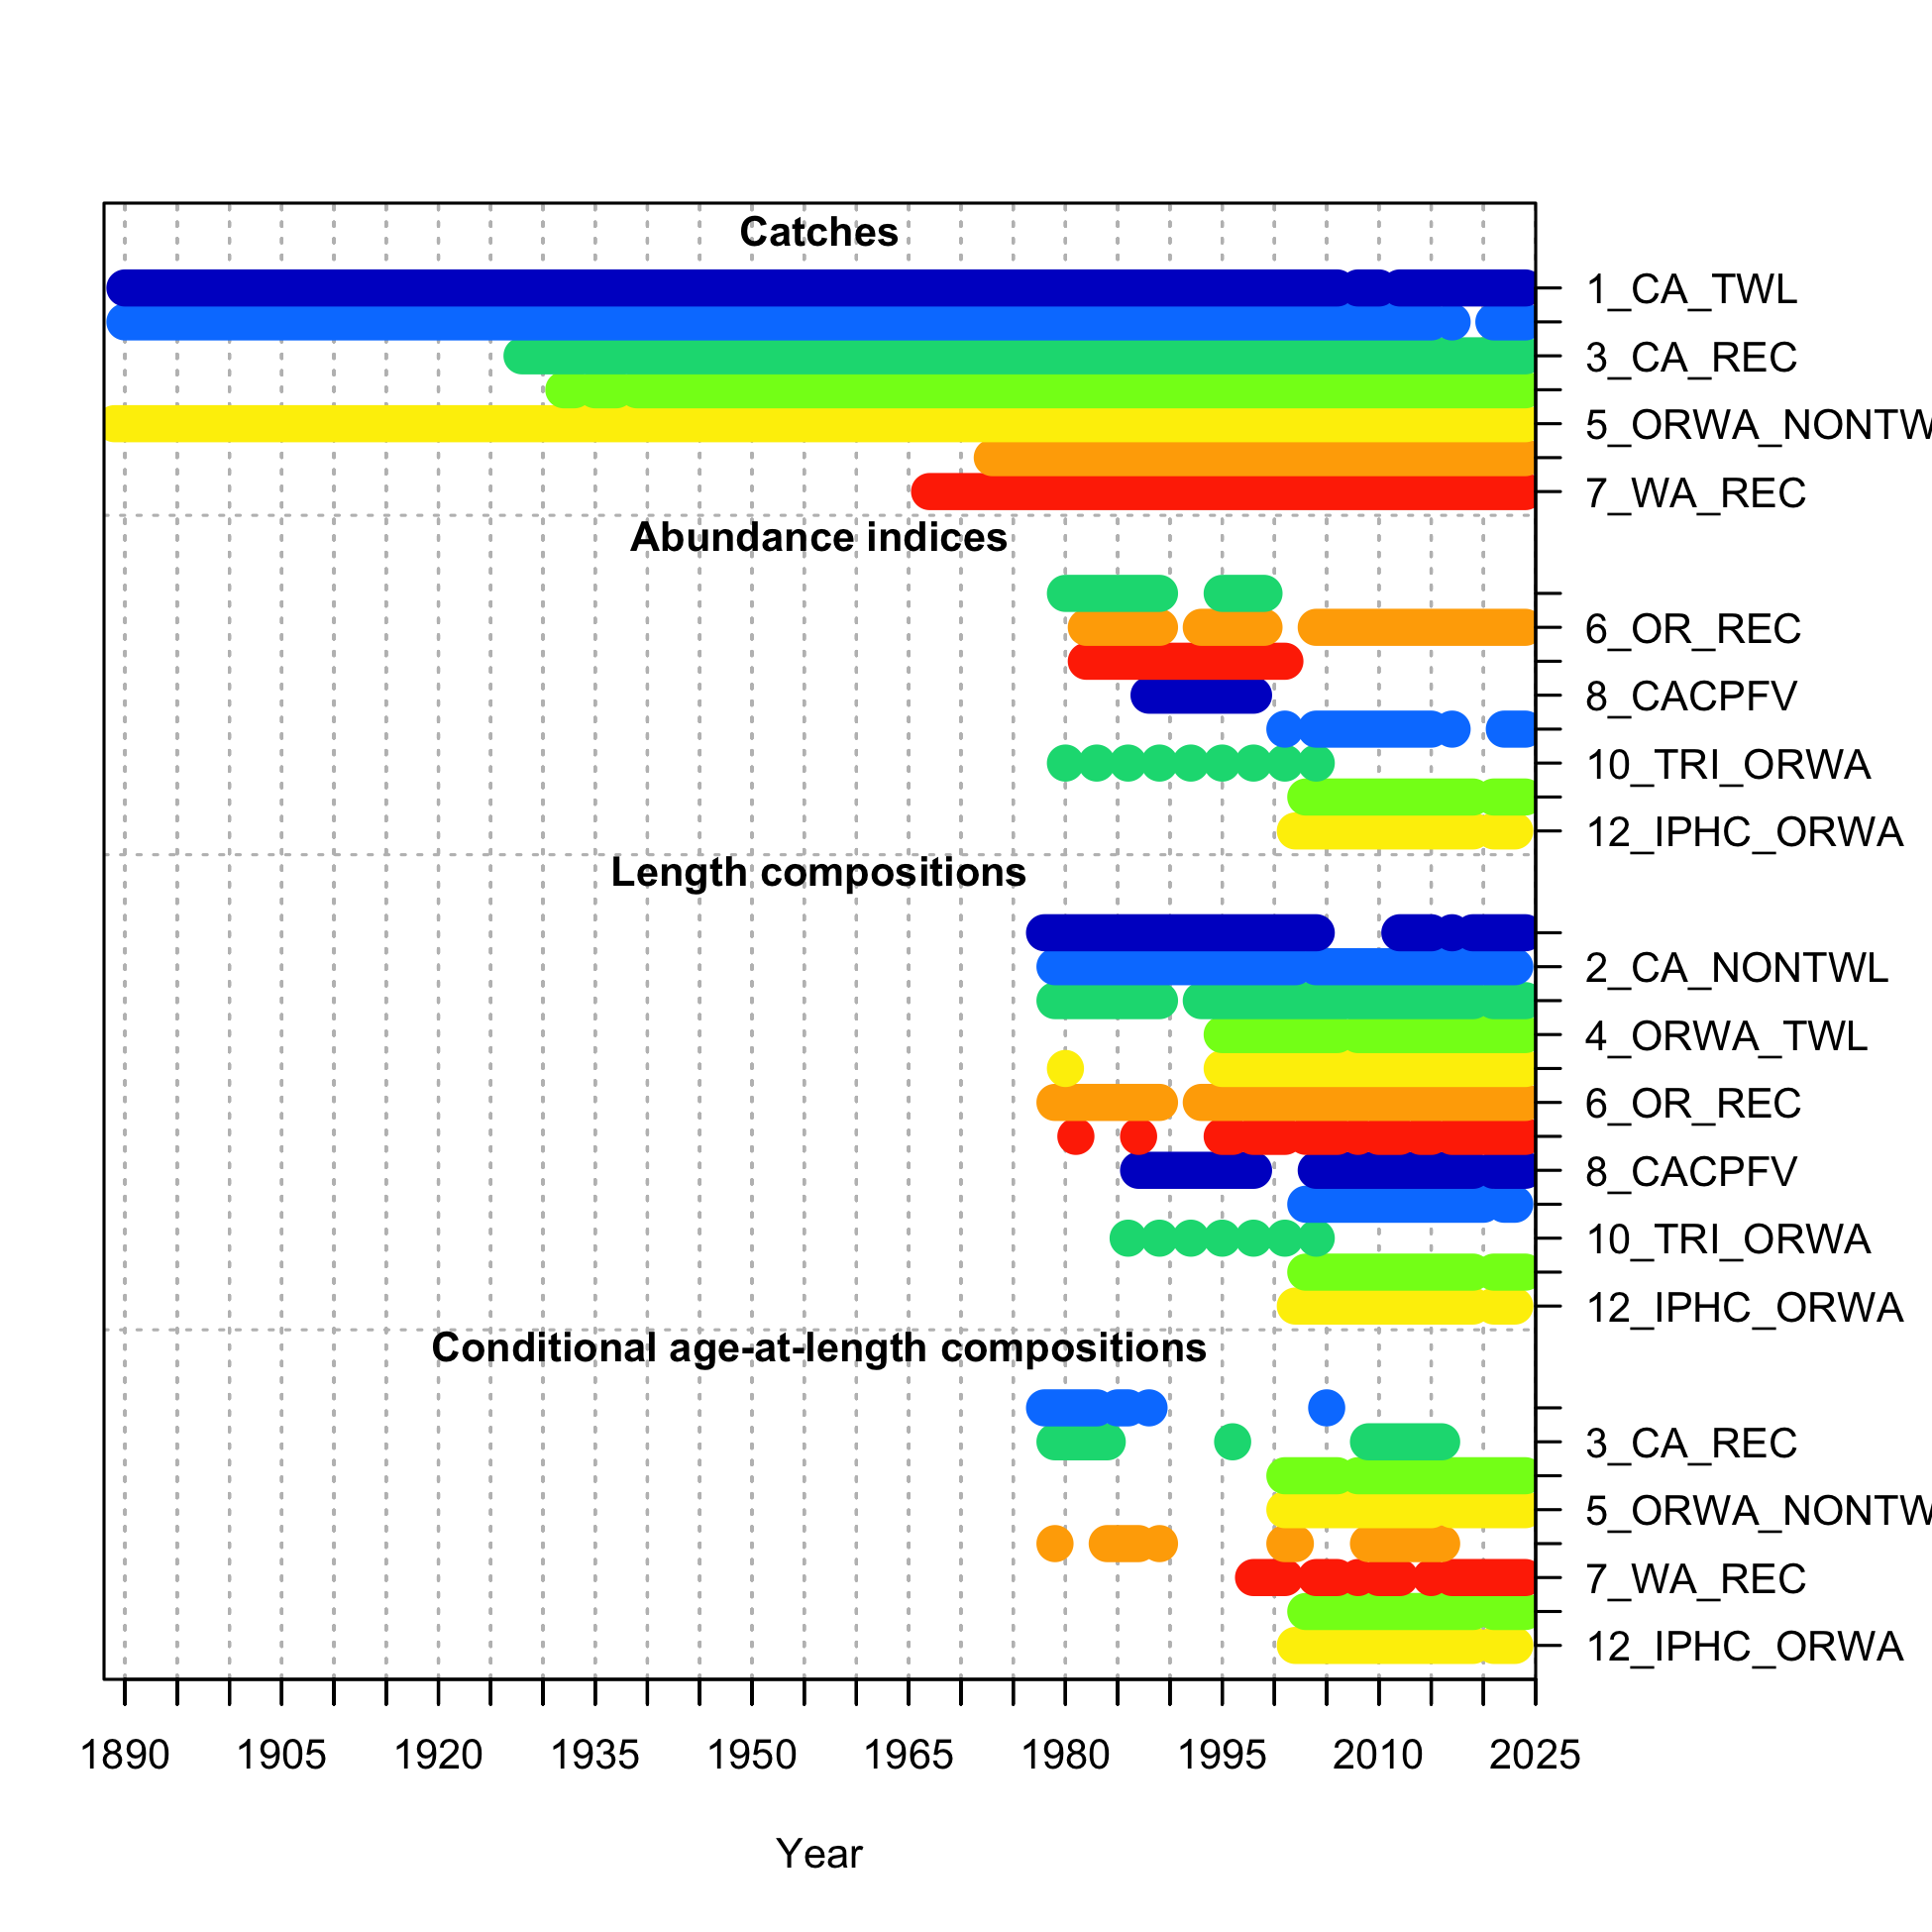
\includegraphics[width=6.5in,height=\textheight,keepaspectratio]{figures/r4ss_plots/plots/data_plot.png}

}

\caption{\label{fig-data}Summary of data sources used in the base
model.}

\end{figure}%

\begin{figure}

\centering{

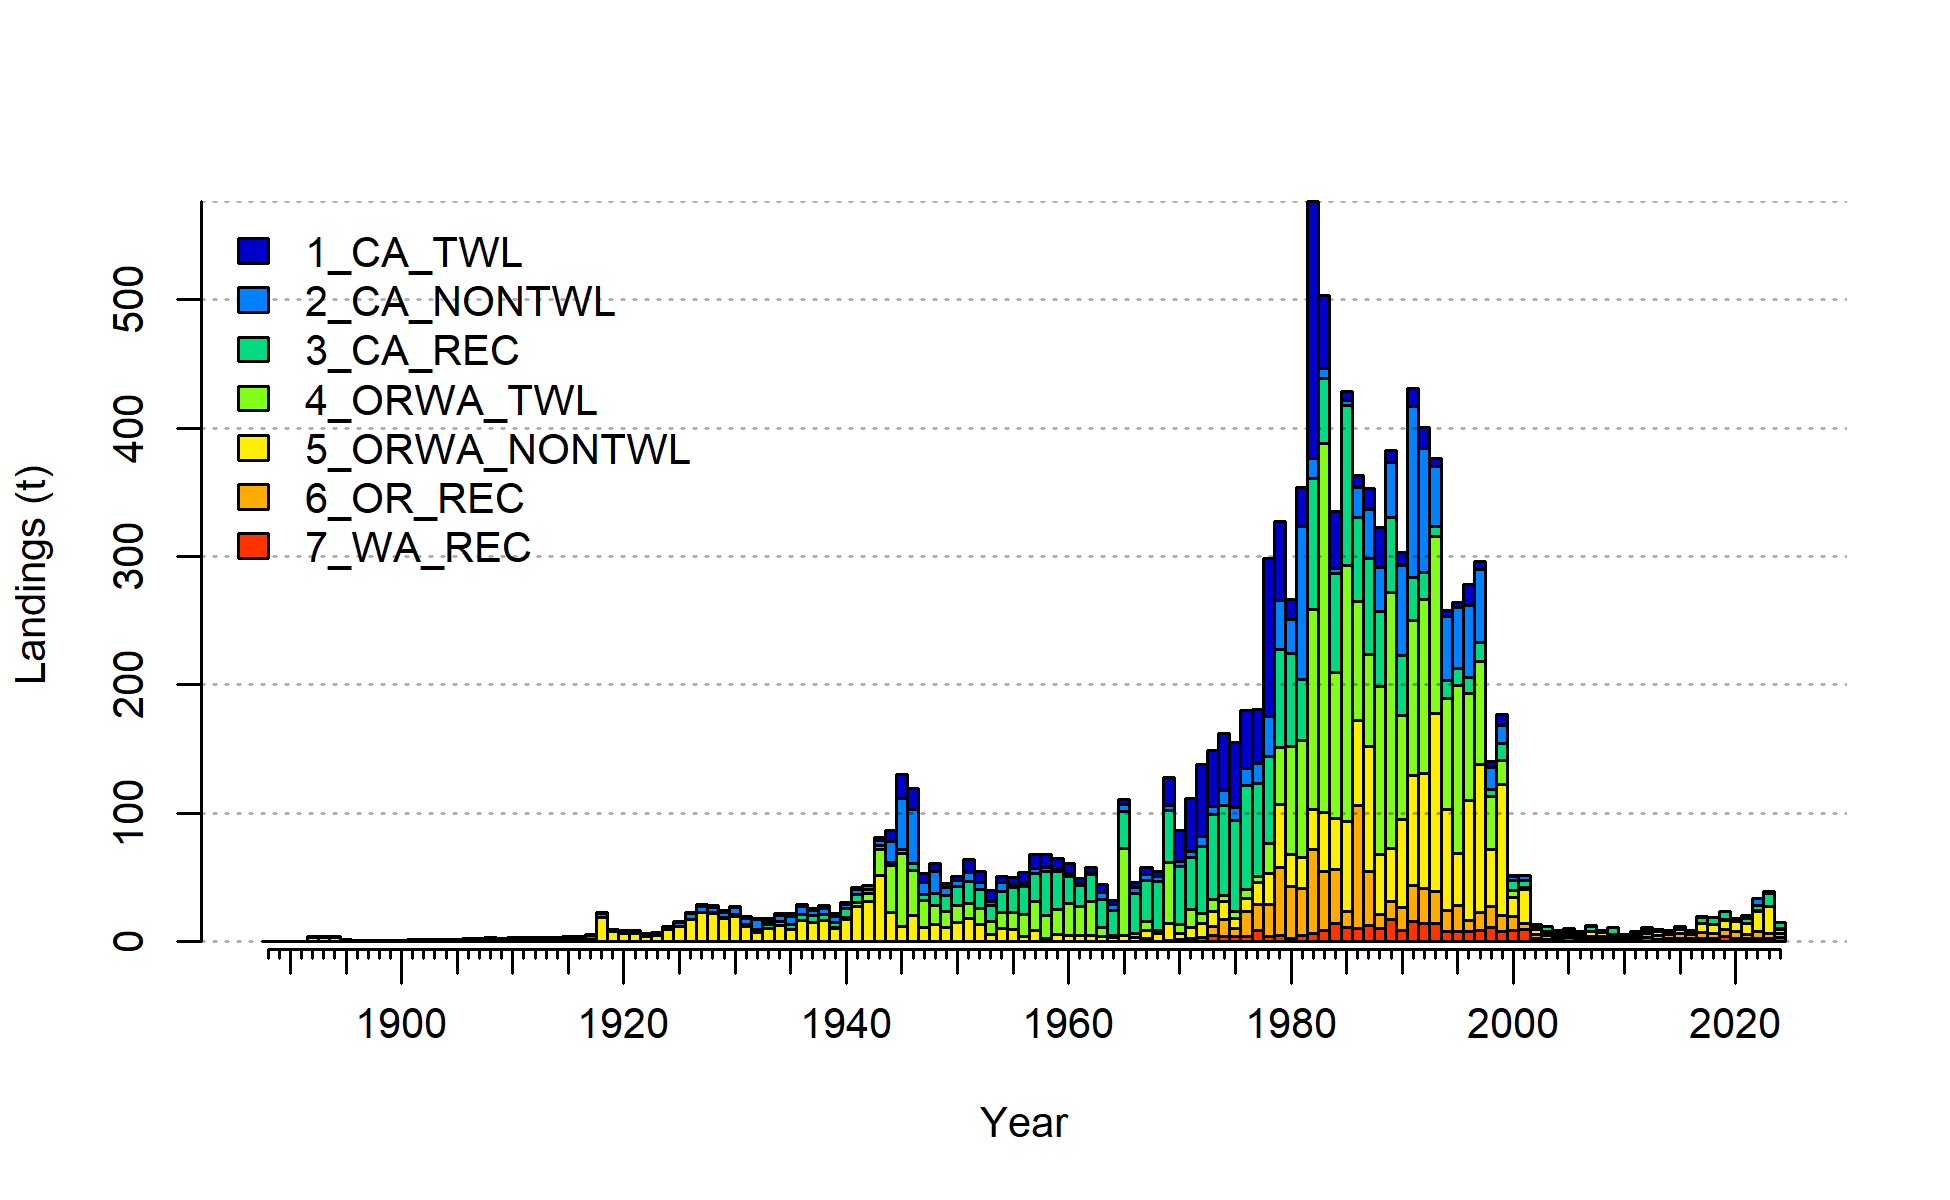
\includegraphics[width=6.5in,height=\textheight,keepaspectratio]{figures/r4ss_plots/plots/catch2_landings_stacked.png}

}

\caption{\label{fig-catch}Landings (mt) by year and fleet.}

\end{figure}%

\begin{figure}

\centering{

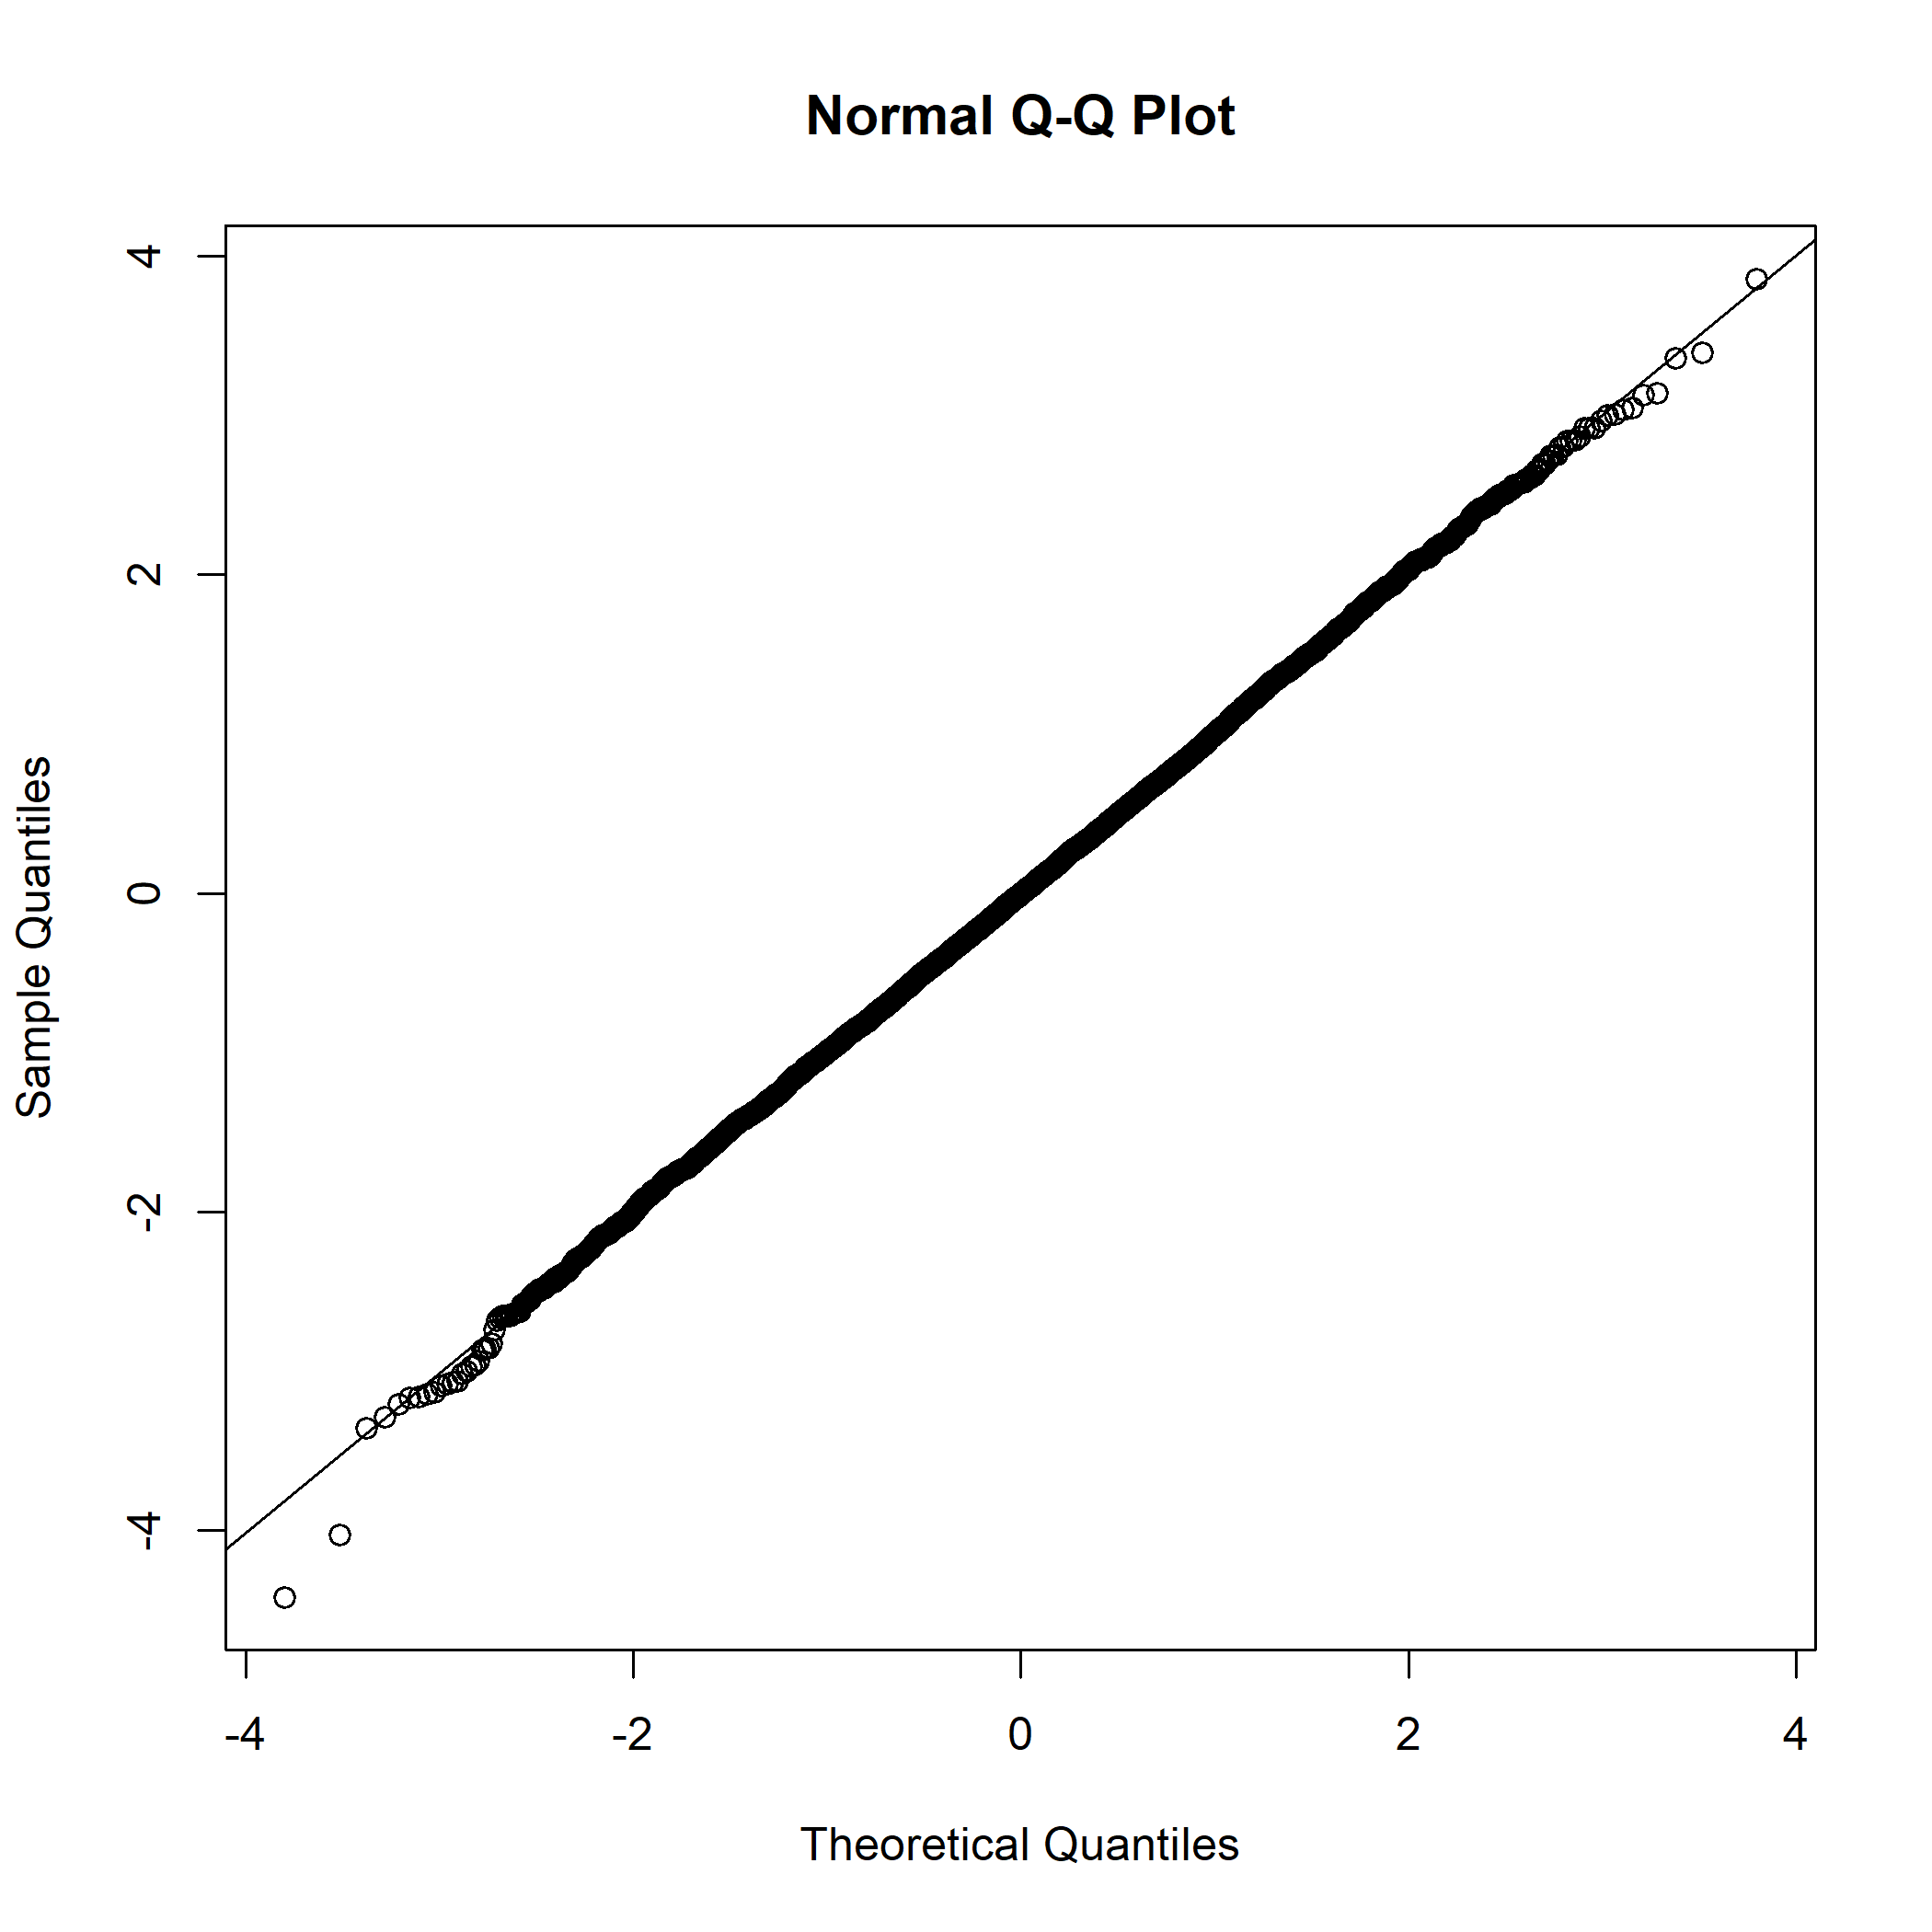
\includegraphics[width=7in,height=\textheight,keepaspectratio]{figures/indices/ORFS_qq.png}

}

\caption{\label{fig-orfs_qqplot}Quantile-quantile plot for the sdmTMB
model fit for the Oregon Onboard Observer (ORFS) index.}

\end{figure}%

\begin{figure}

\centering{

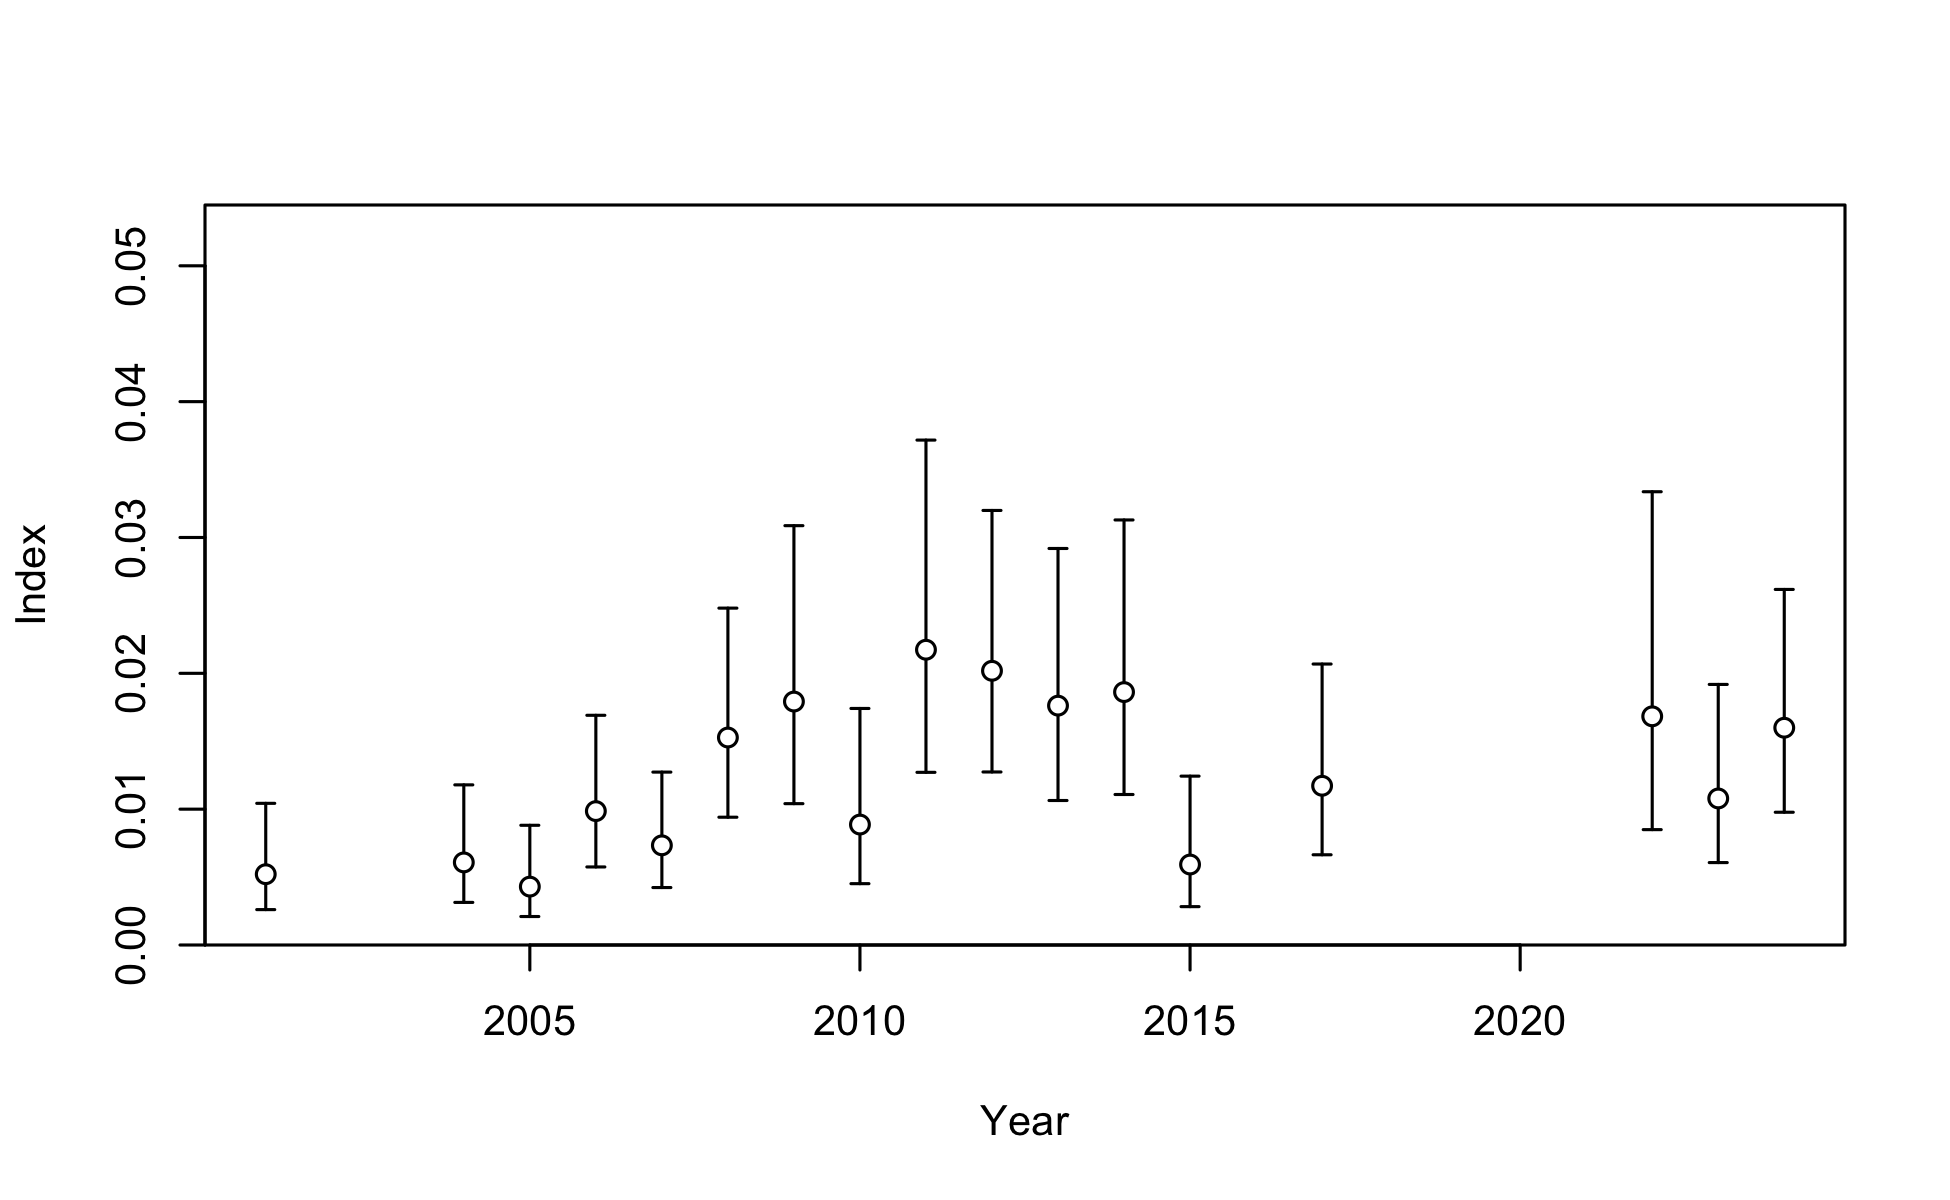
\includegraphics[width=6.5in,height=\textheight,keepaspectratio]{figures/r4ss_plots/plots/index1_cpuedata_9_OR_RECOB.png}

}

\caption{\label{fig-ORFS_index}Annual relative index of abundance for
the Oregon Onboard Observer (ORFS) index.}

\end{figure}%

\begin{figure}

\centering{

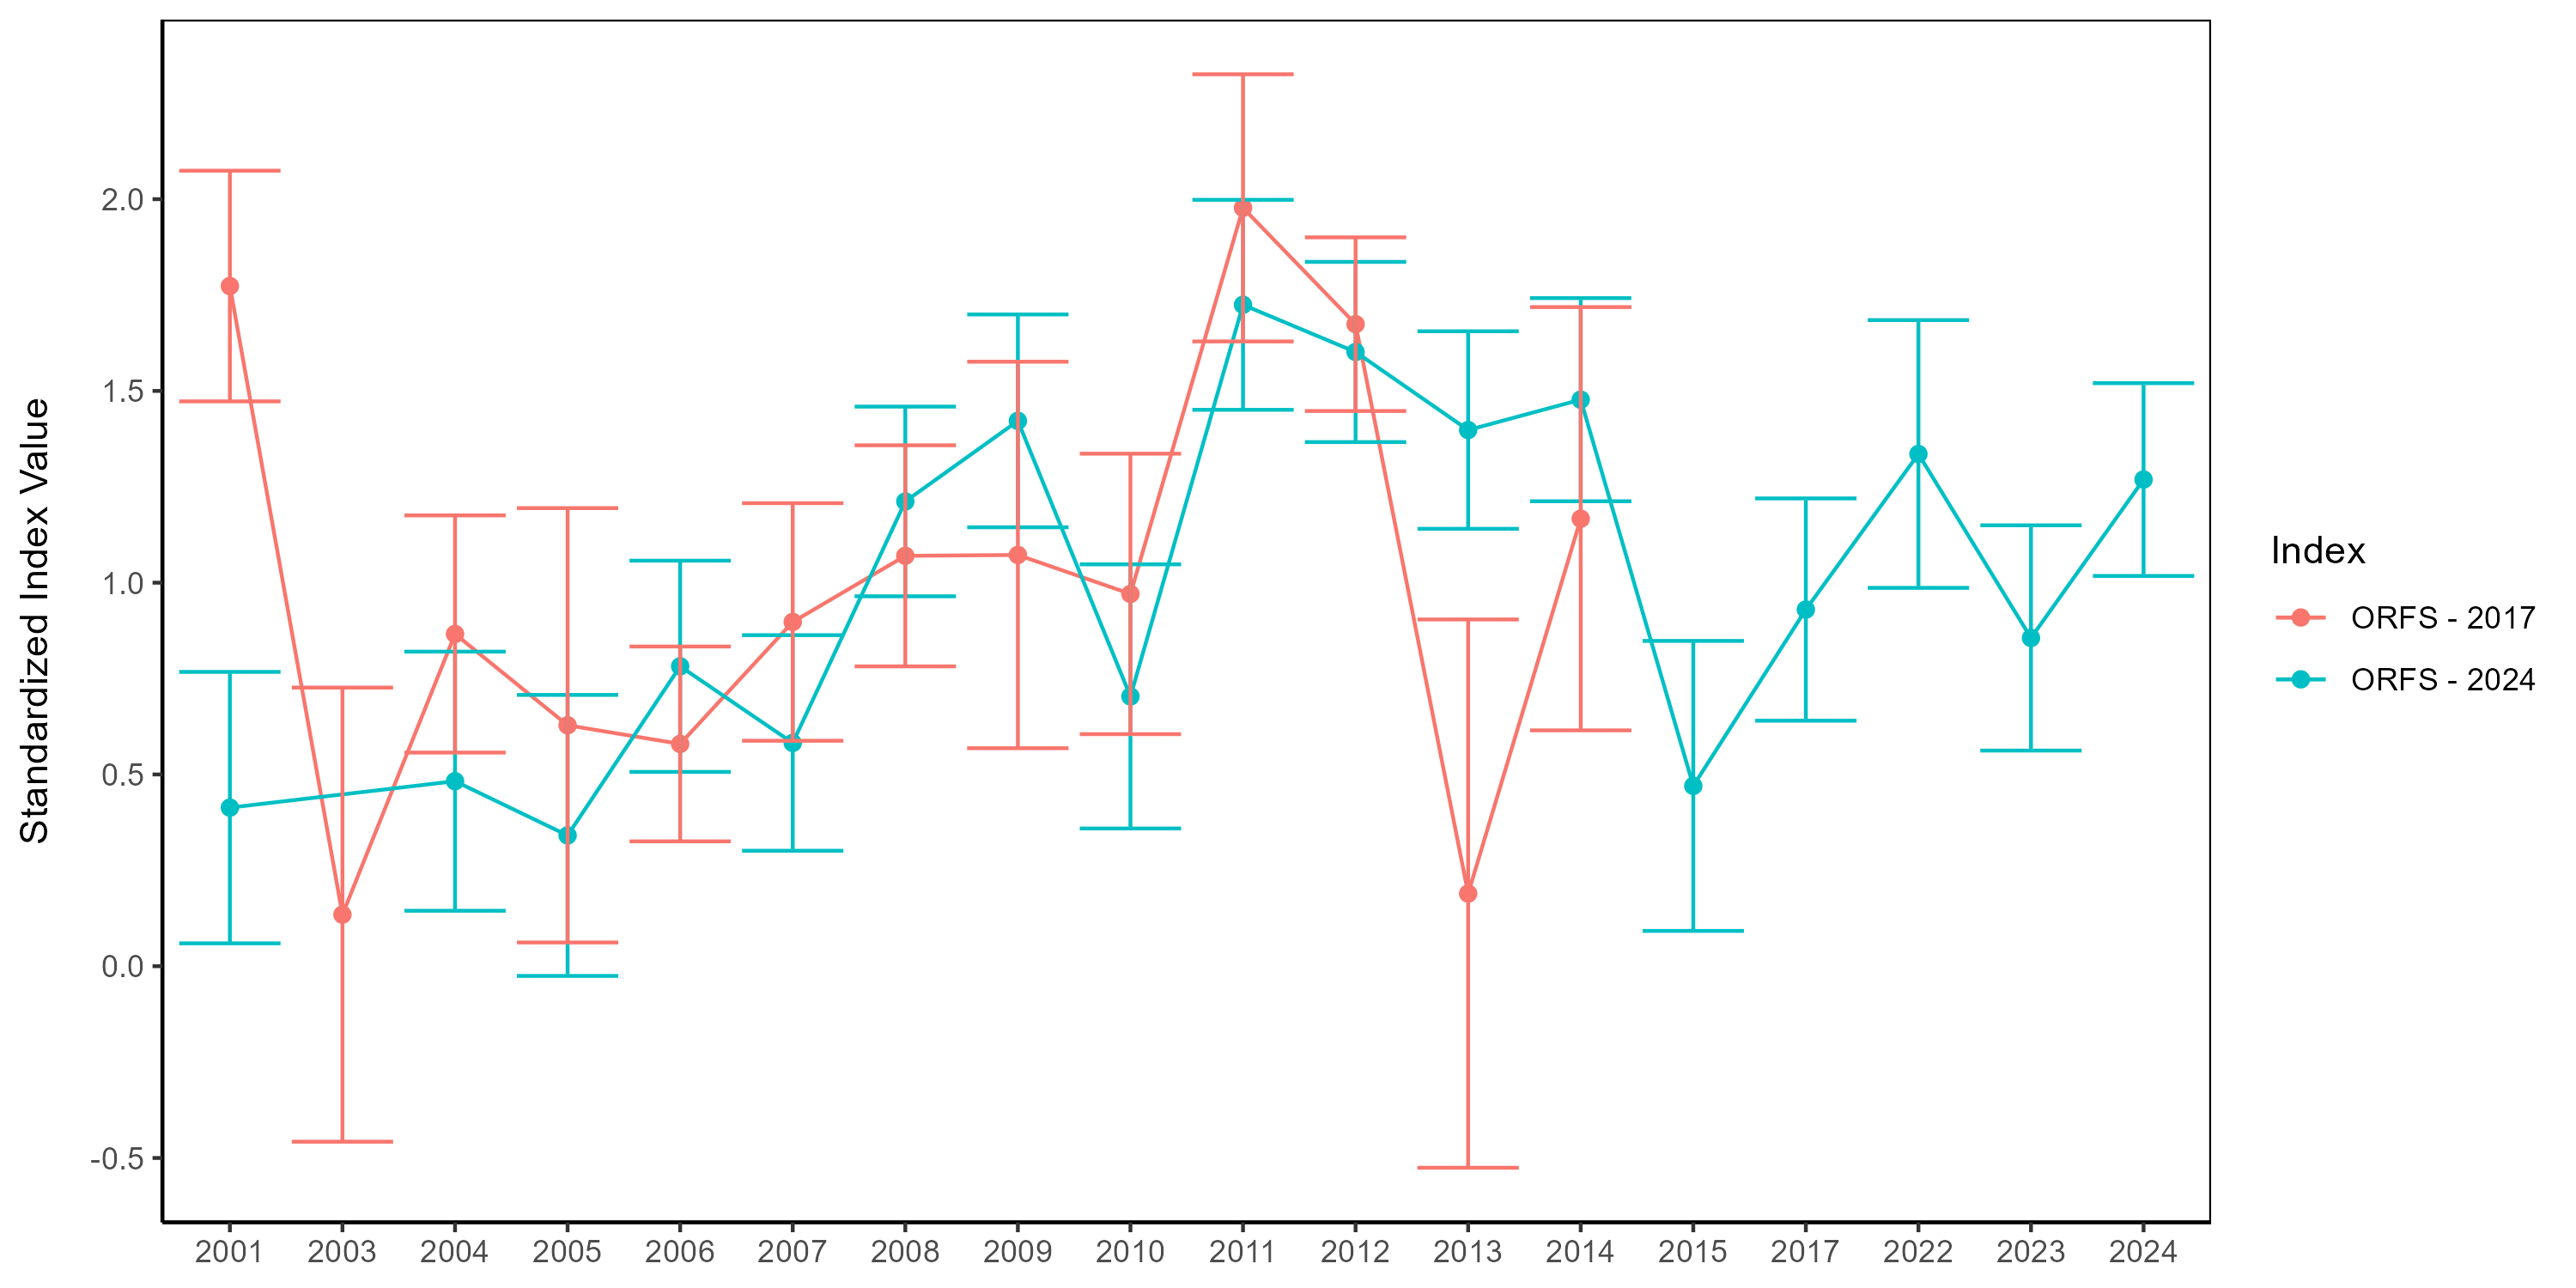
\includegraphics[width=10in,height=\textheight,keepaspectratio]{figures/indices/ORFS index comparison_errbars.png}

}

\caption{\label{fig-ORFS_comp}Comparison of Oregon Onboard Observer
indices from the 2017 and the current assessment.}

\end{figure}%

\begin{figure}

\centering{

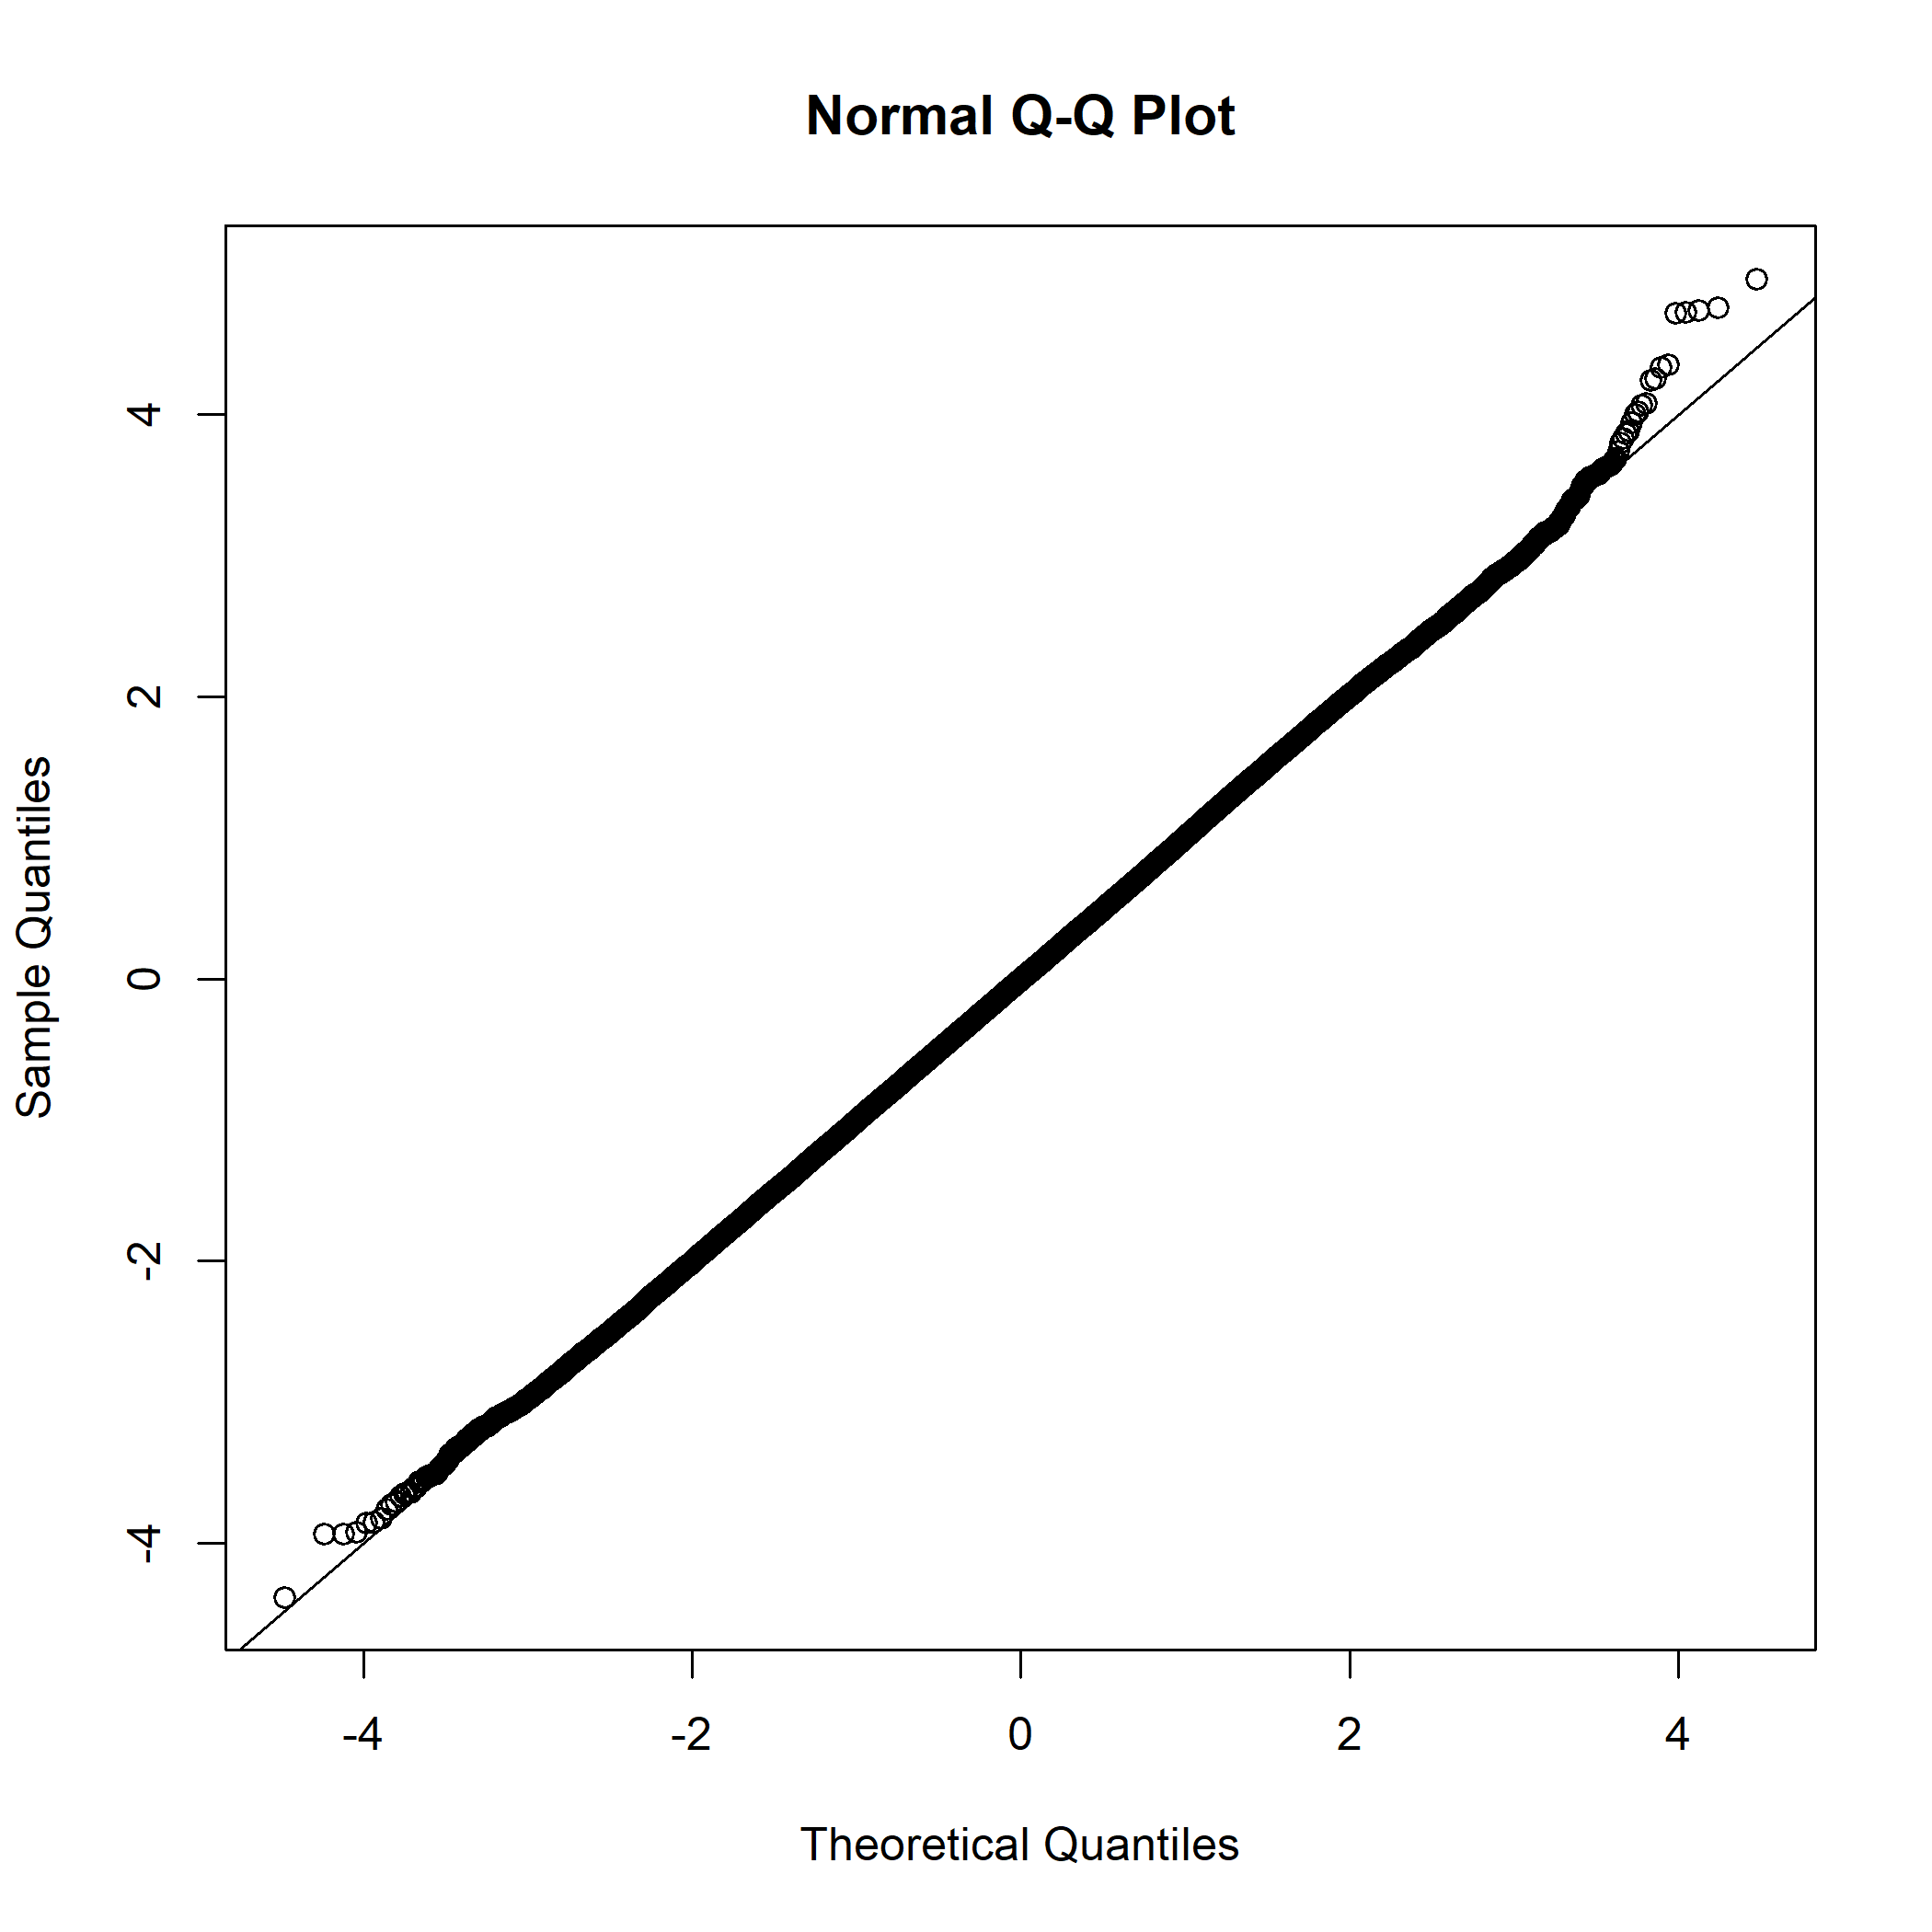
\includegraphics[width=7in,height=\textheight,keepaspectratio]{figures/indices/ORBS_qq.png}

}

\caption{\label{fig-orbs_qq}Quantile-quantile plot for the sdmTMB model
fit for the updated portion of the Oregon recreational (ORBS) index.}

\end{figure}%

\begin{figure}

\centering{

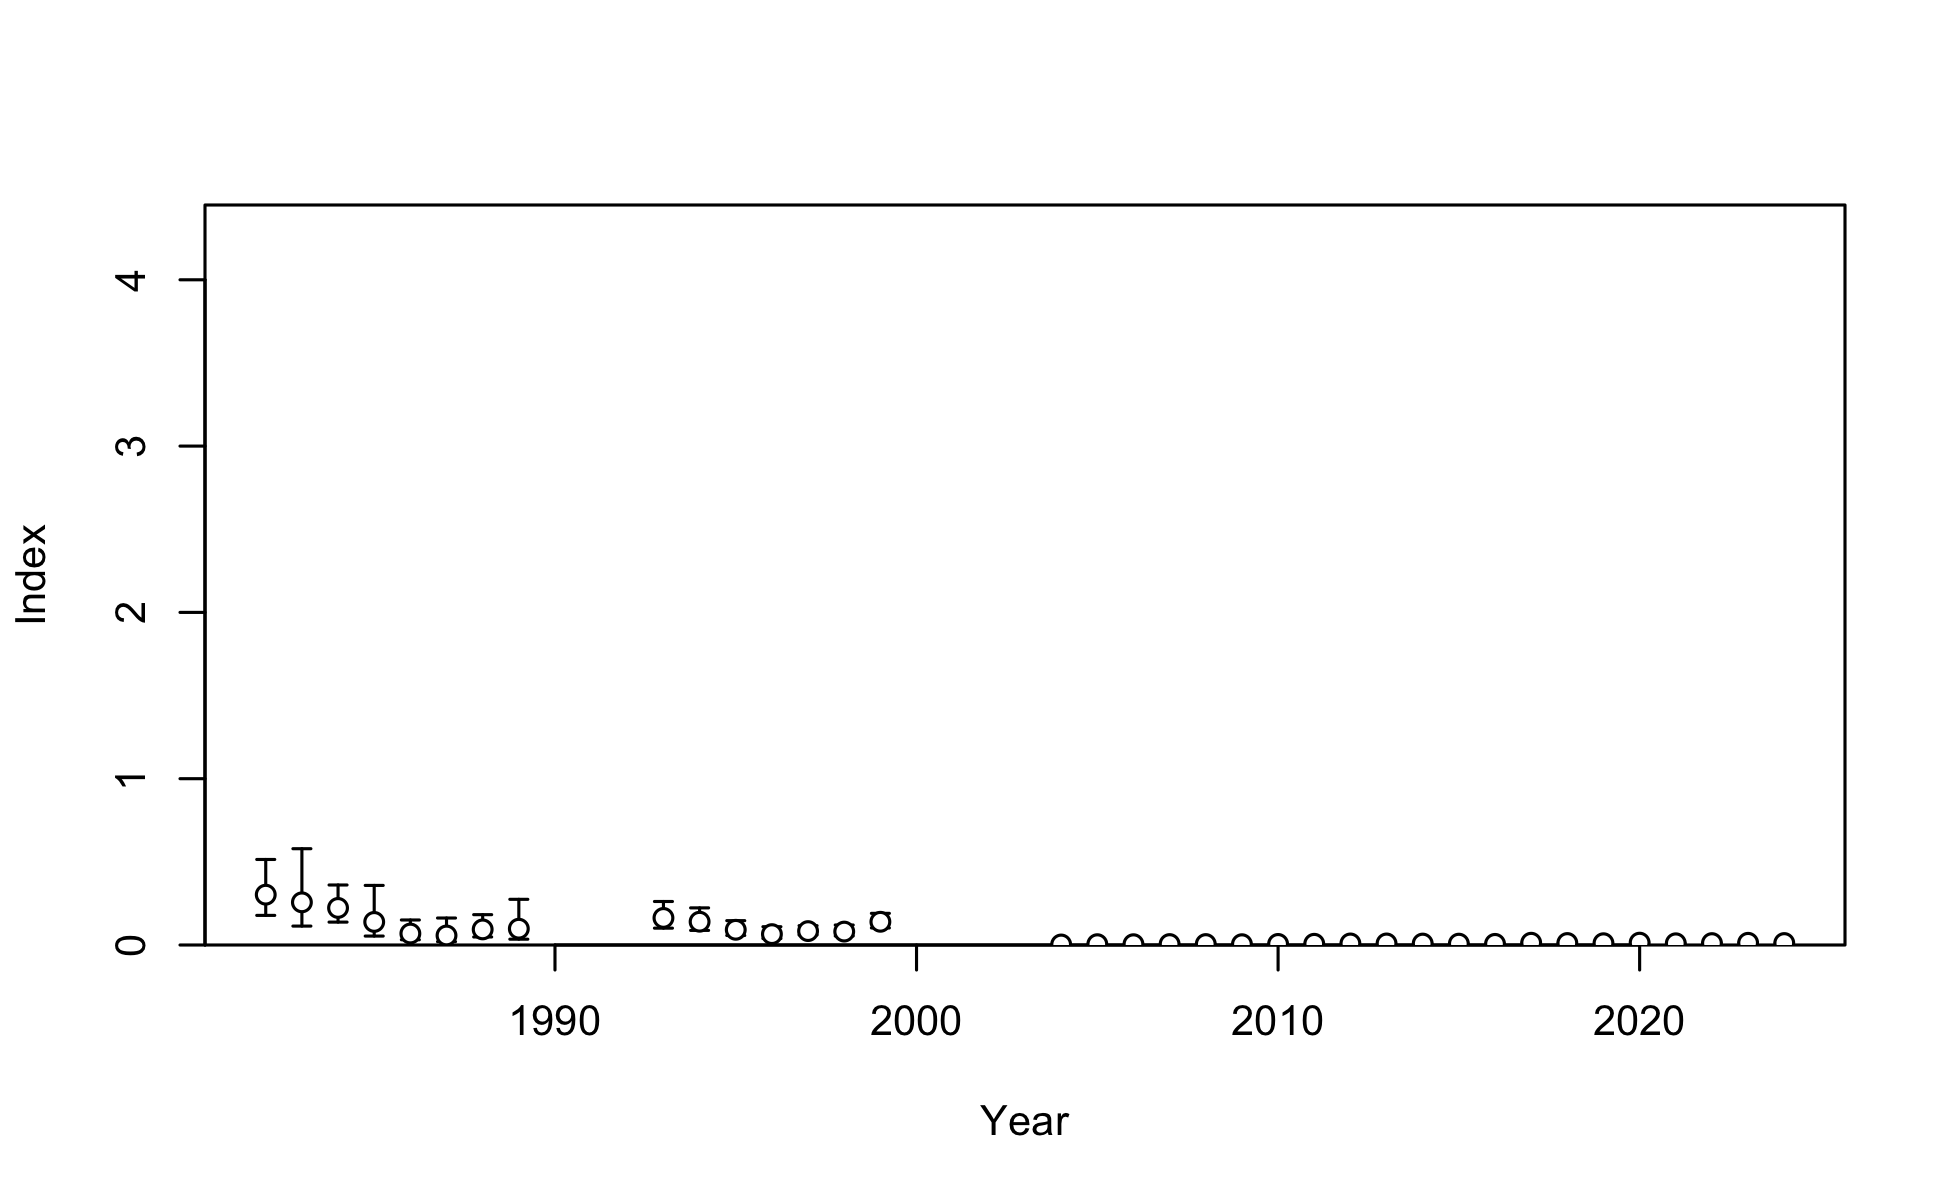
\includegraphics[width=6.5in,height=\textheight,keepaspectratio]{figures/r4ss_plots/plots/index1_cpuedata_6_OR_REC.png}

}

\caption{\label{fig-ORBS_index}Annual relative index of abundance for
the Oregon recreational index, including both MRFSS (1980 - 1999) and
ORBS (2004 - 2024) indices.}

\end{figure}%

\clearpage

\begin{figure}

\centering{

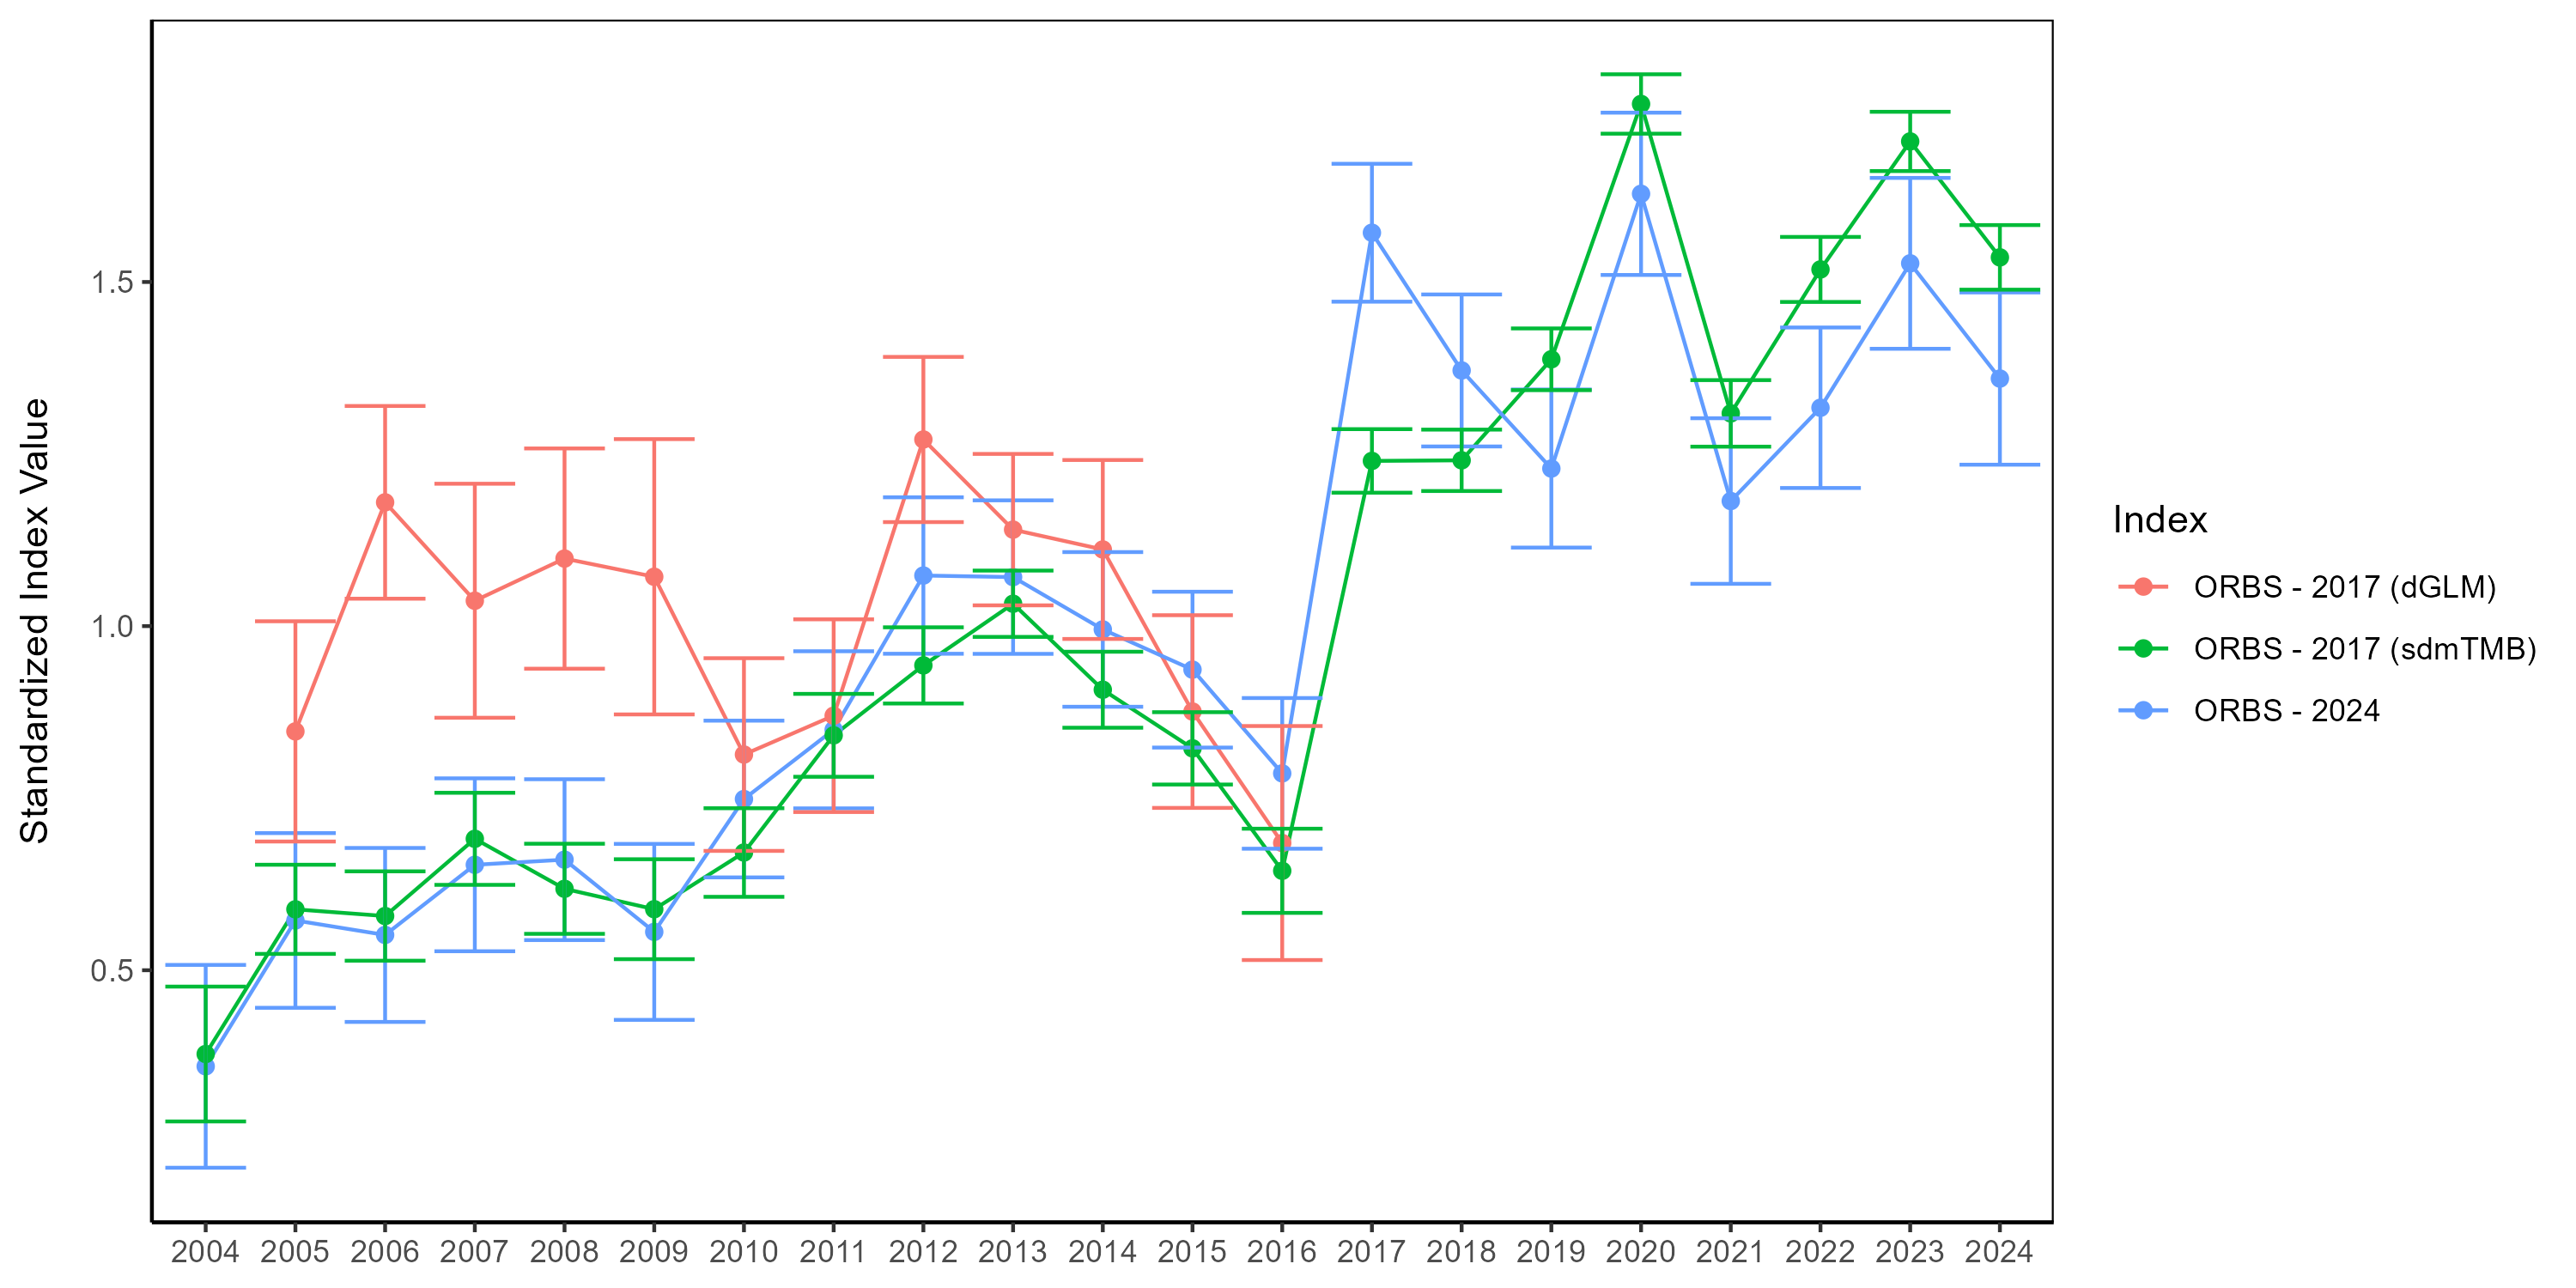
\includegraphics[width=10in,height=\textheight,keepaspectratio]{figures/indices/ORBS index comparison_ORBSonly_errbars.png}

}

\caption{\label{fig-ORBS_comp}Comparison of the 2017 ORBS index
(delta-GLM), the 2017 ORBS model (implemented in sdmTMB), and the
current ORBS index (sdmTMB).}

\end{figure}%

\begin{figure}

\centering{

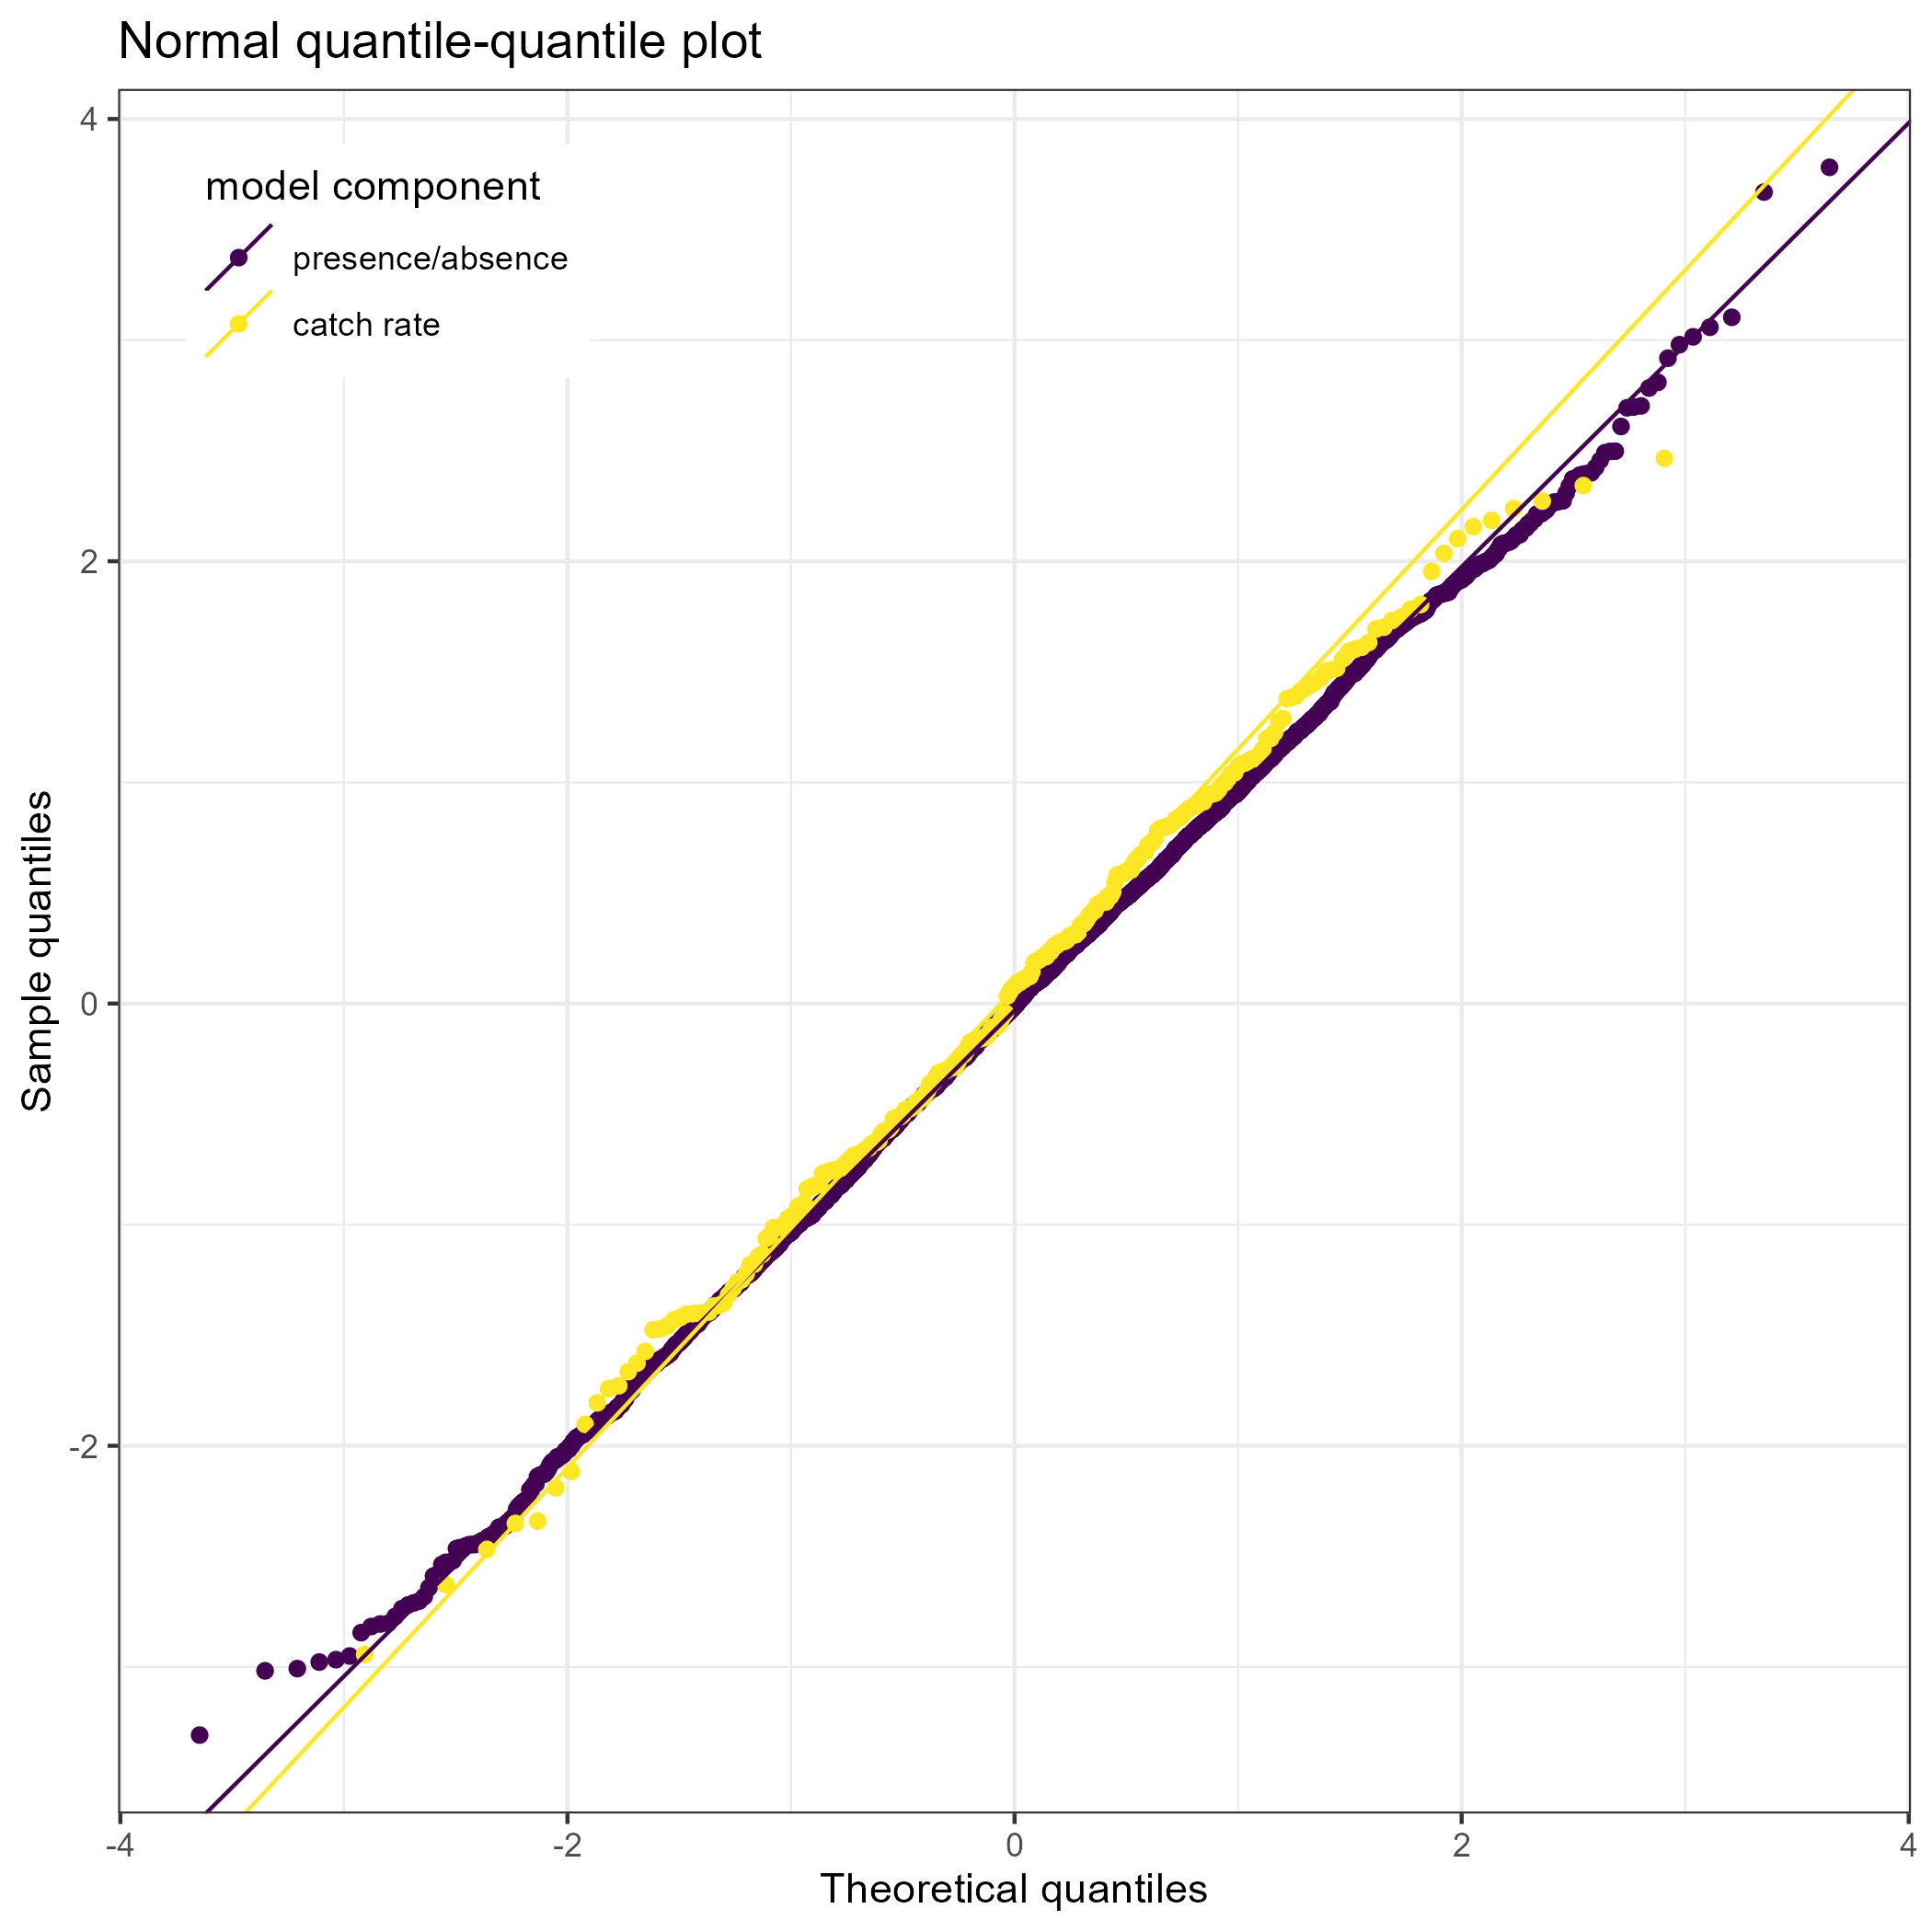
\includegraphics[width=7in,height=\textheight,keepaspectratio]{figures/indices/wcgbts_qq.png}

}

\caption{\label{fig-wcgbts_qq}Quantile-quantile plot for the sdmTMB
model fit for the NWFSC West Coast Groundfish Bottom Trawl Survey
(WCGBTS) index.}

\end{figure}%

\begin{figure}

\centering{

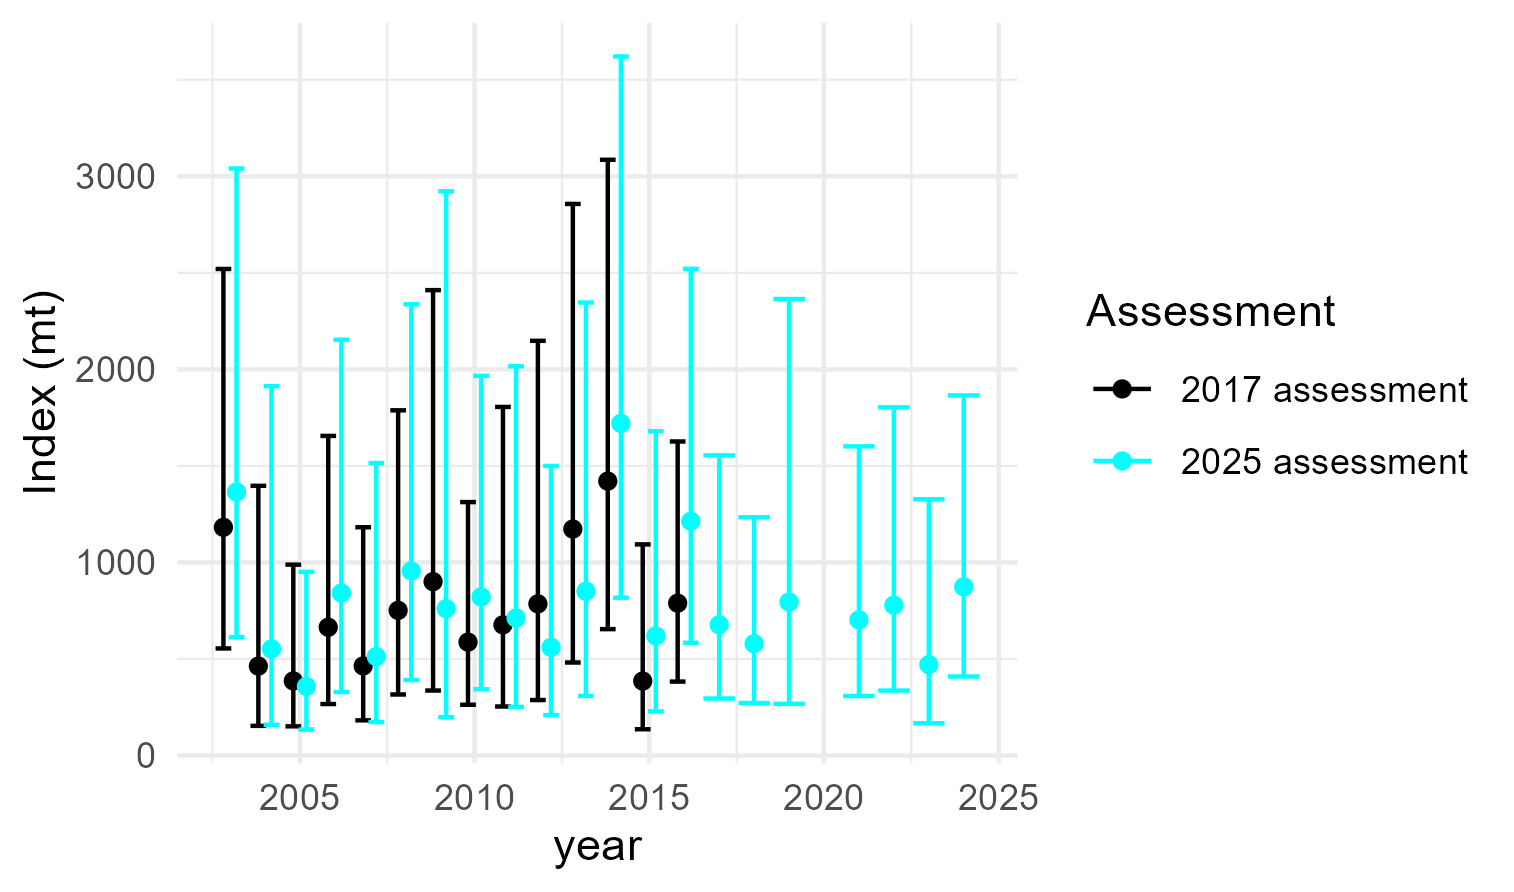
\includegraphics[width=5.05in,height=\textheight,keepaspectratio]{figures/indices/wcgbts_index_comparison.png}

}

\caption{\label{fig-wcgbtsindexcomparison}Comparison of the 2017 NWFSC
West Coast Groundfish Bottom Trawl Survey (WCGBTS) and the current WCBTS
index of abundance.}

\end{figure}%

\begin{figure}

\centering{

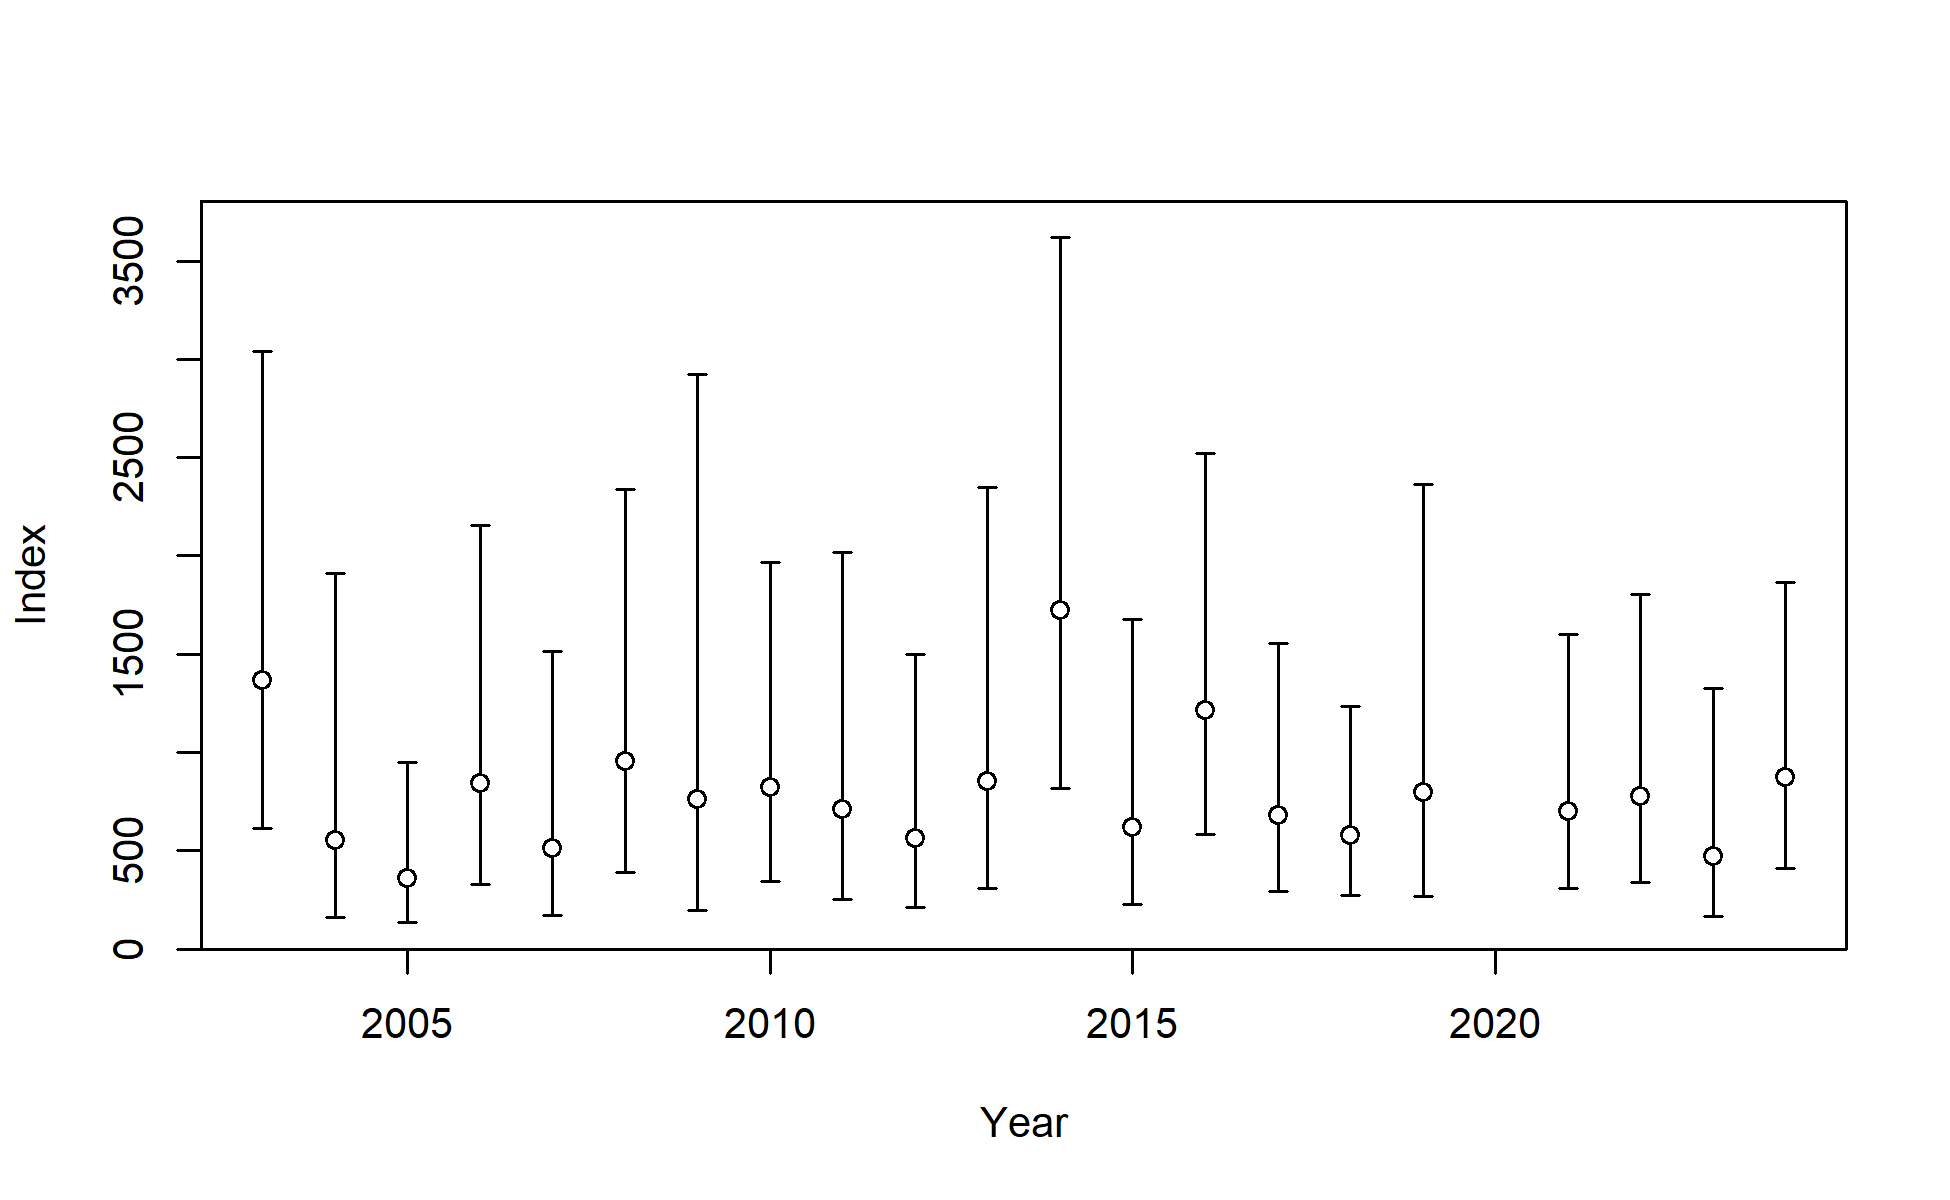
\includegraphics[width=6.5in,height=\textheight,keepaspectratio]{figures/r4ss_plots/plots/index1_cpuedata_11_NWFSC_ORWA.png}

}

\caption{\label{fig-wcgbtsindex}Annual relative index of abundance for
the West Coast Groundfish Bottom Trawl Survey (WCGBTS).}

\end{figure}%

\begin{figure}

\centering{

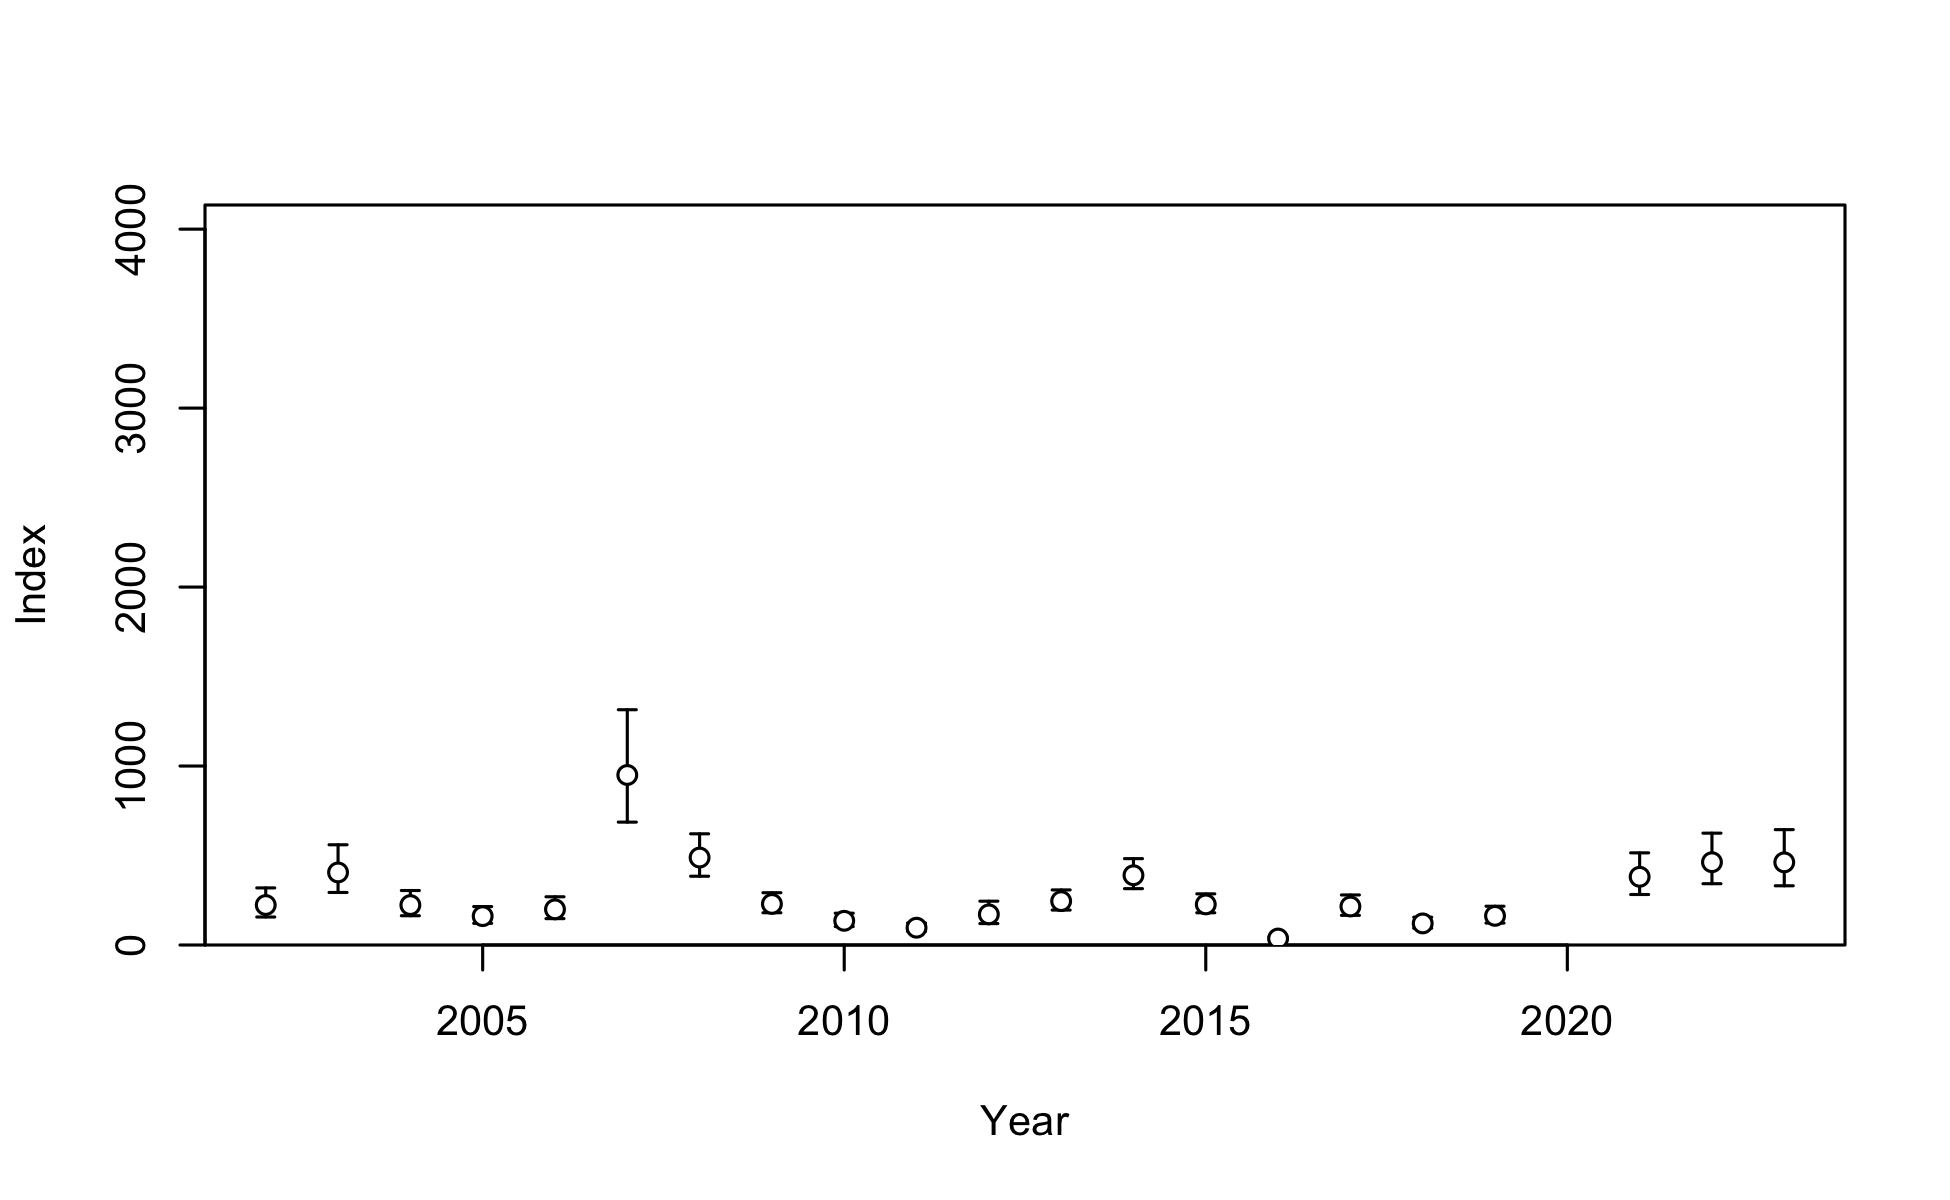
\includegraphics[width=6.5in,height=\textheight,keepaspectratio]{figures/r4ss_plots/plots/index1_cpuedata_12_IPHC_ORWA.png}

}

\caption{\label{fig-IPHC_index}Annual relative index of abundance for
the IPHC longline survey.}

\end{figure}%

\begin{figure}

\centering{

\pandocbounded{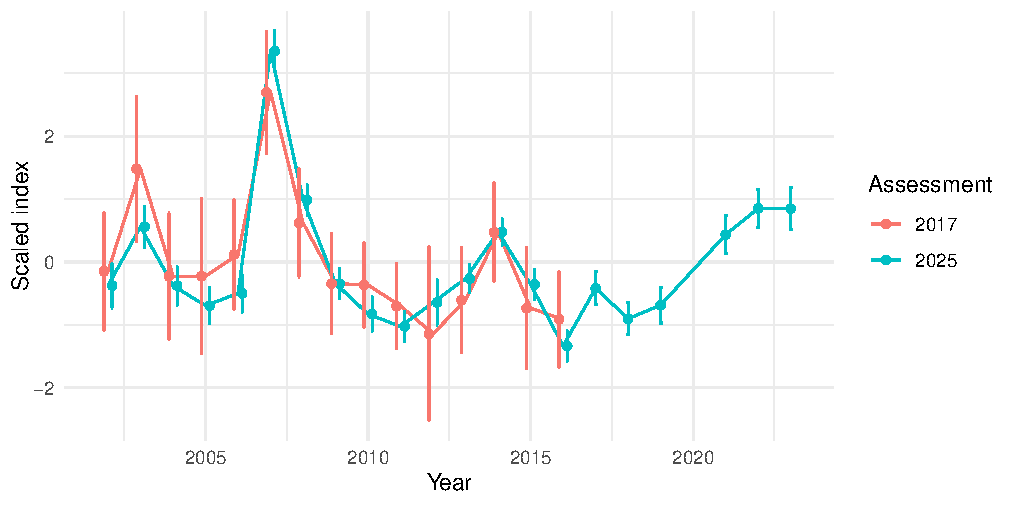
\includegraphics[keepaspectratio]{figures/indices/IPHC_index_comparison.pdf}}

}

\caption{\label{fig-IPHC_comparison}Comparison of the 2017 and the
current IPHC index of abundance.}

\end{figure}%

\begin{figure}

\centering{

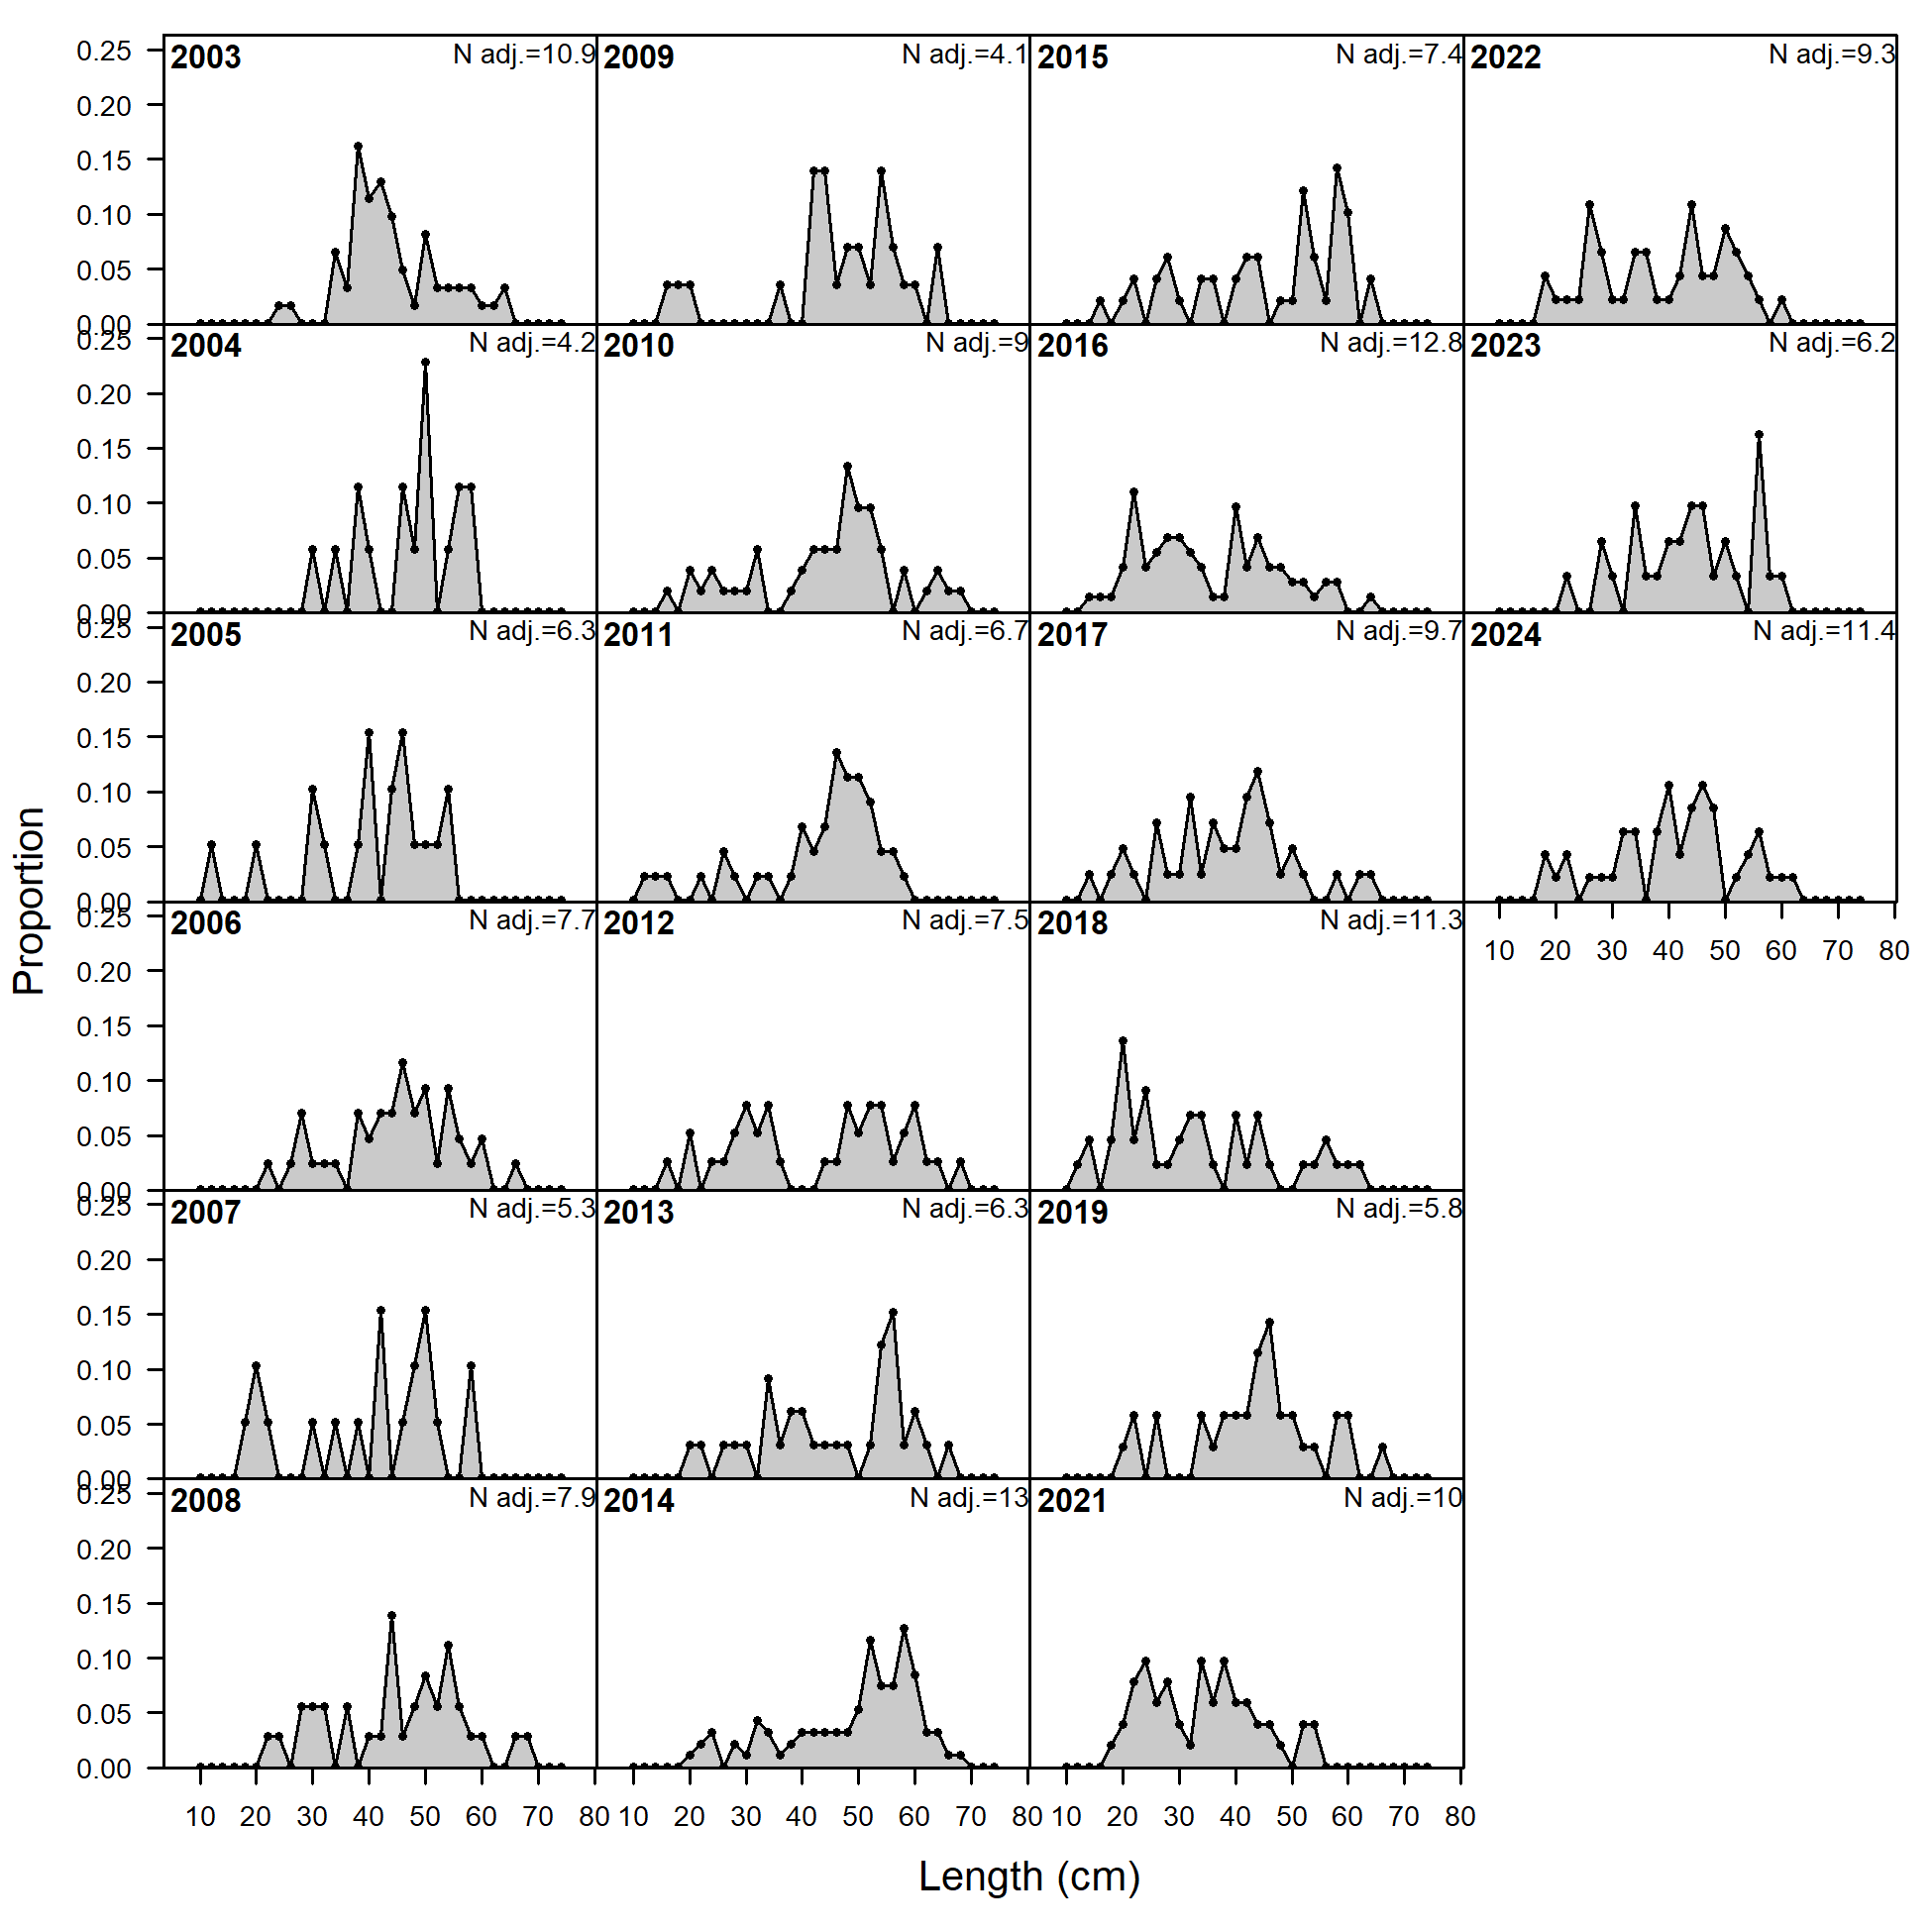
\includegraphics[width=6.5in,height=\textheight,keepaspectratio]{figures/r4ss_plots/plots/comp_lendat_flt11mkt0.png}

}

\caption{\label{fig-NWFSC_lencomps}Annual length composition data for
the WCBTS.}

\end{figure}%

\begin{figure}

\centering{

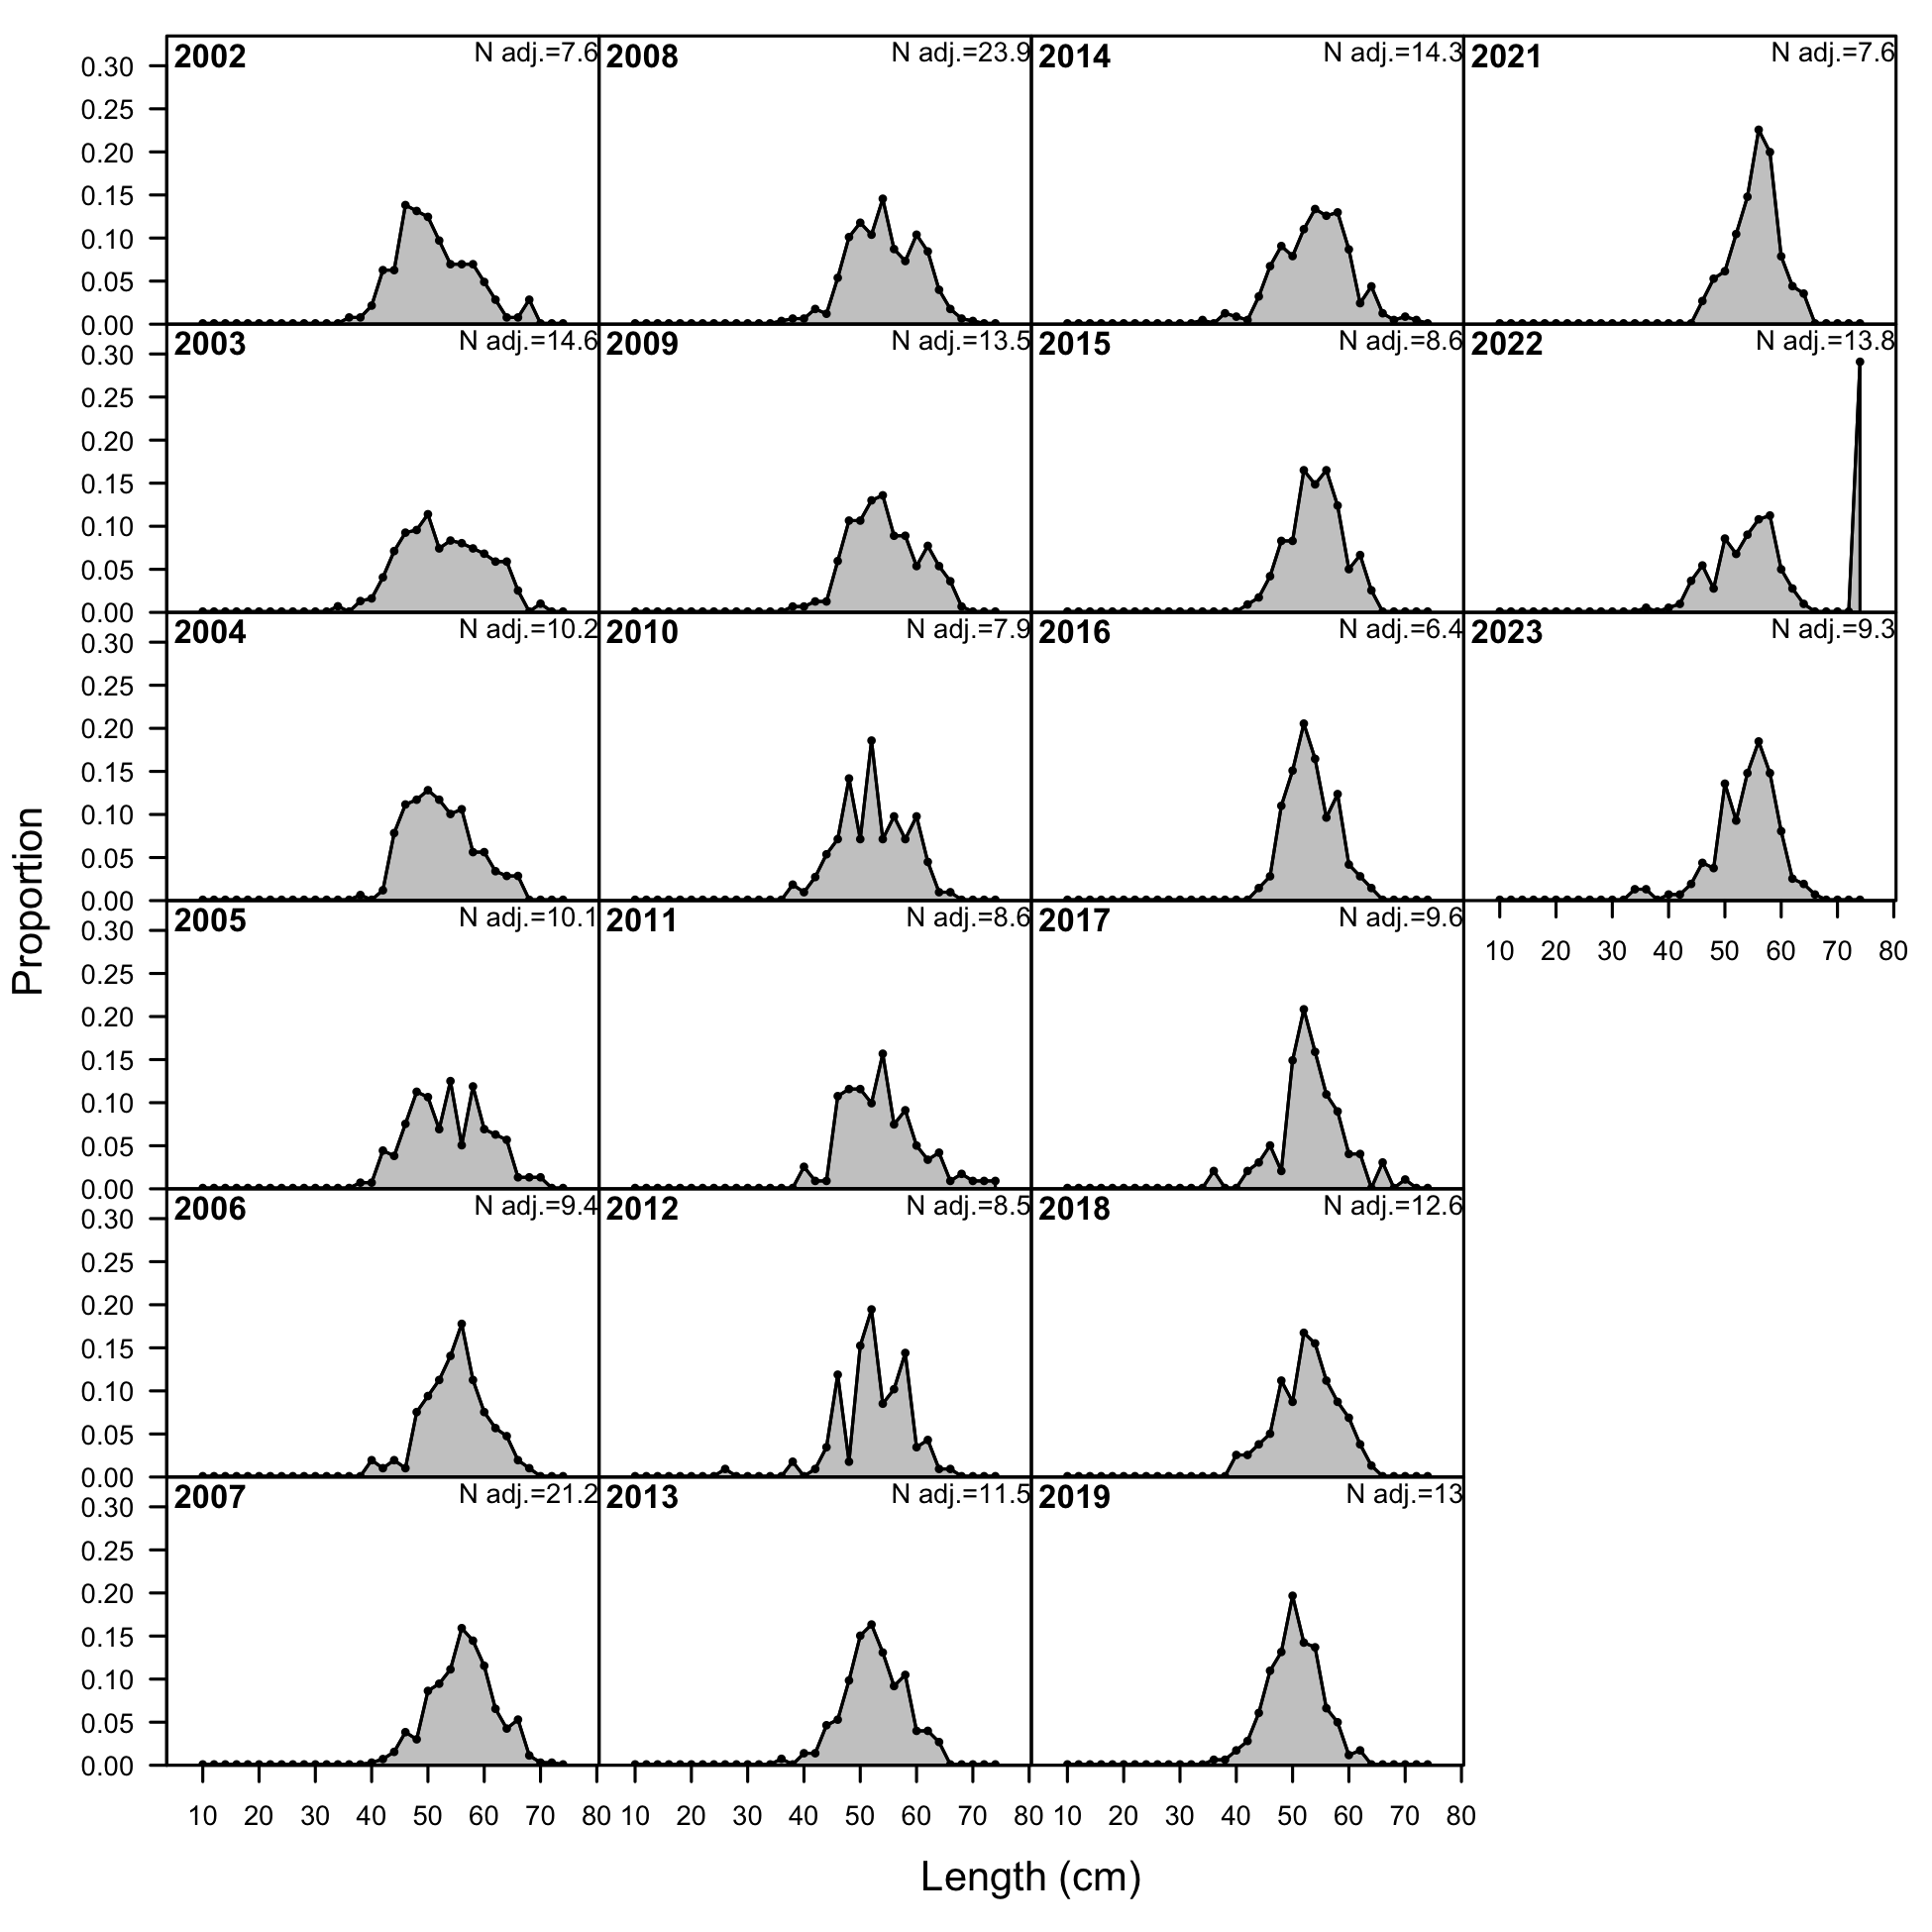
\includegraphics[width=6.5in,height=\textheight,keepaspectratio]{figures/r4ss_plots/plots/comp_lendat_flt12mkt0.png}

}

\caption{\label{fig-IPHC_lencomps}Annual length composition data from
the IPHC longline survey.}

\end{figure}%

\clearpage

\begin{figure}

\centering{

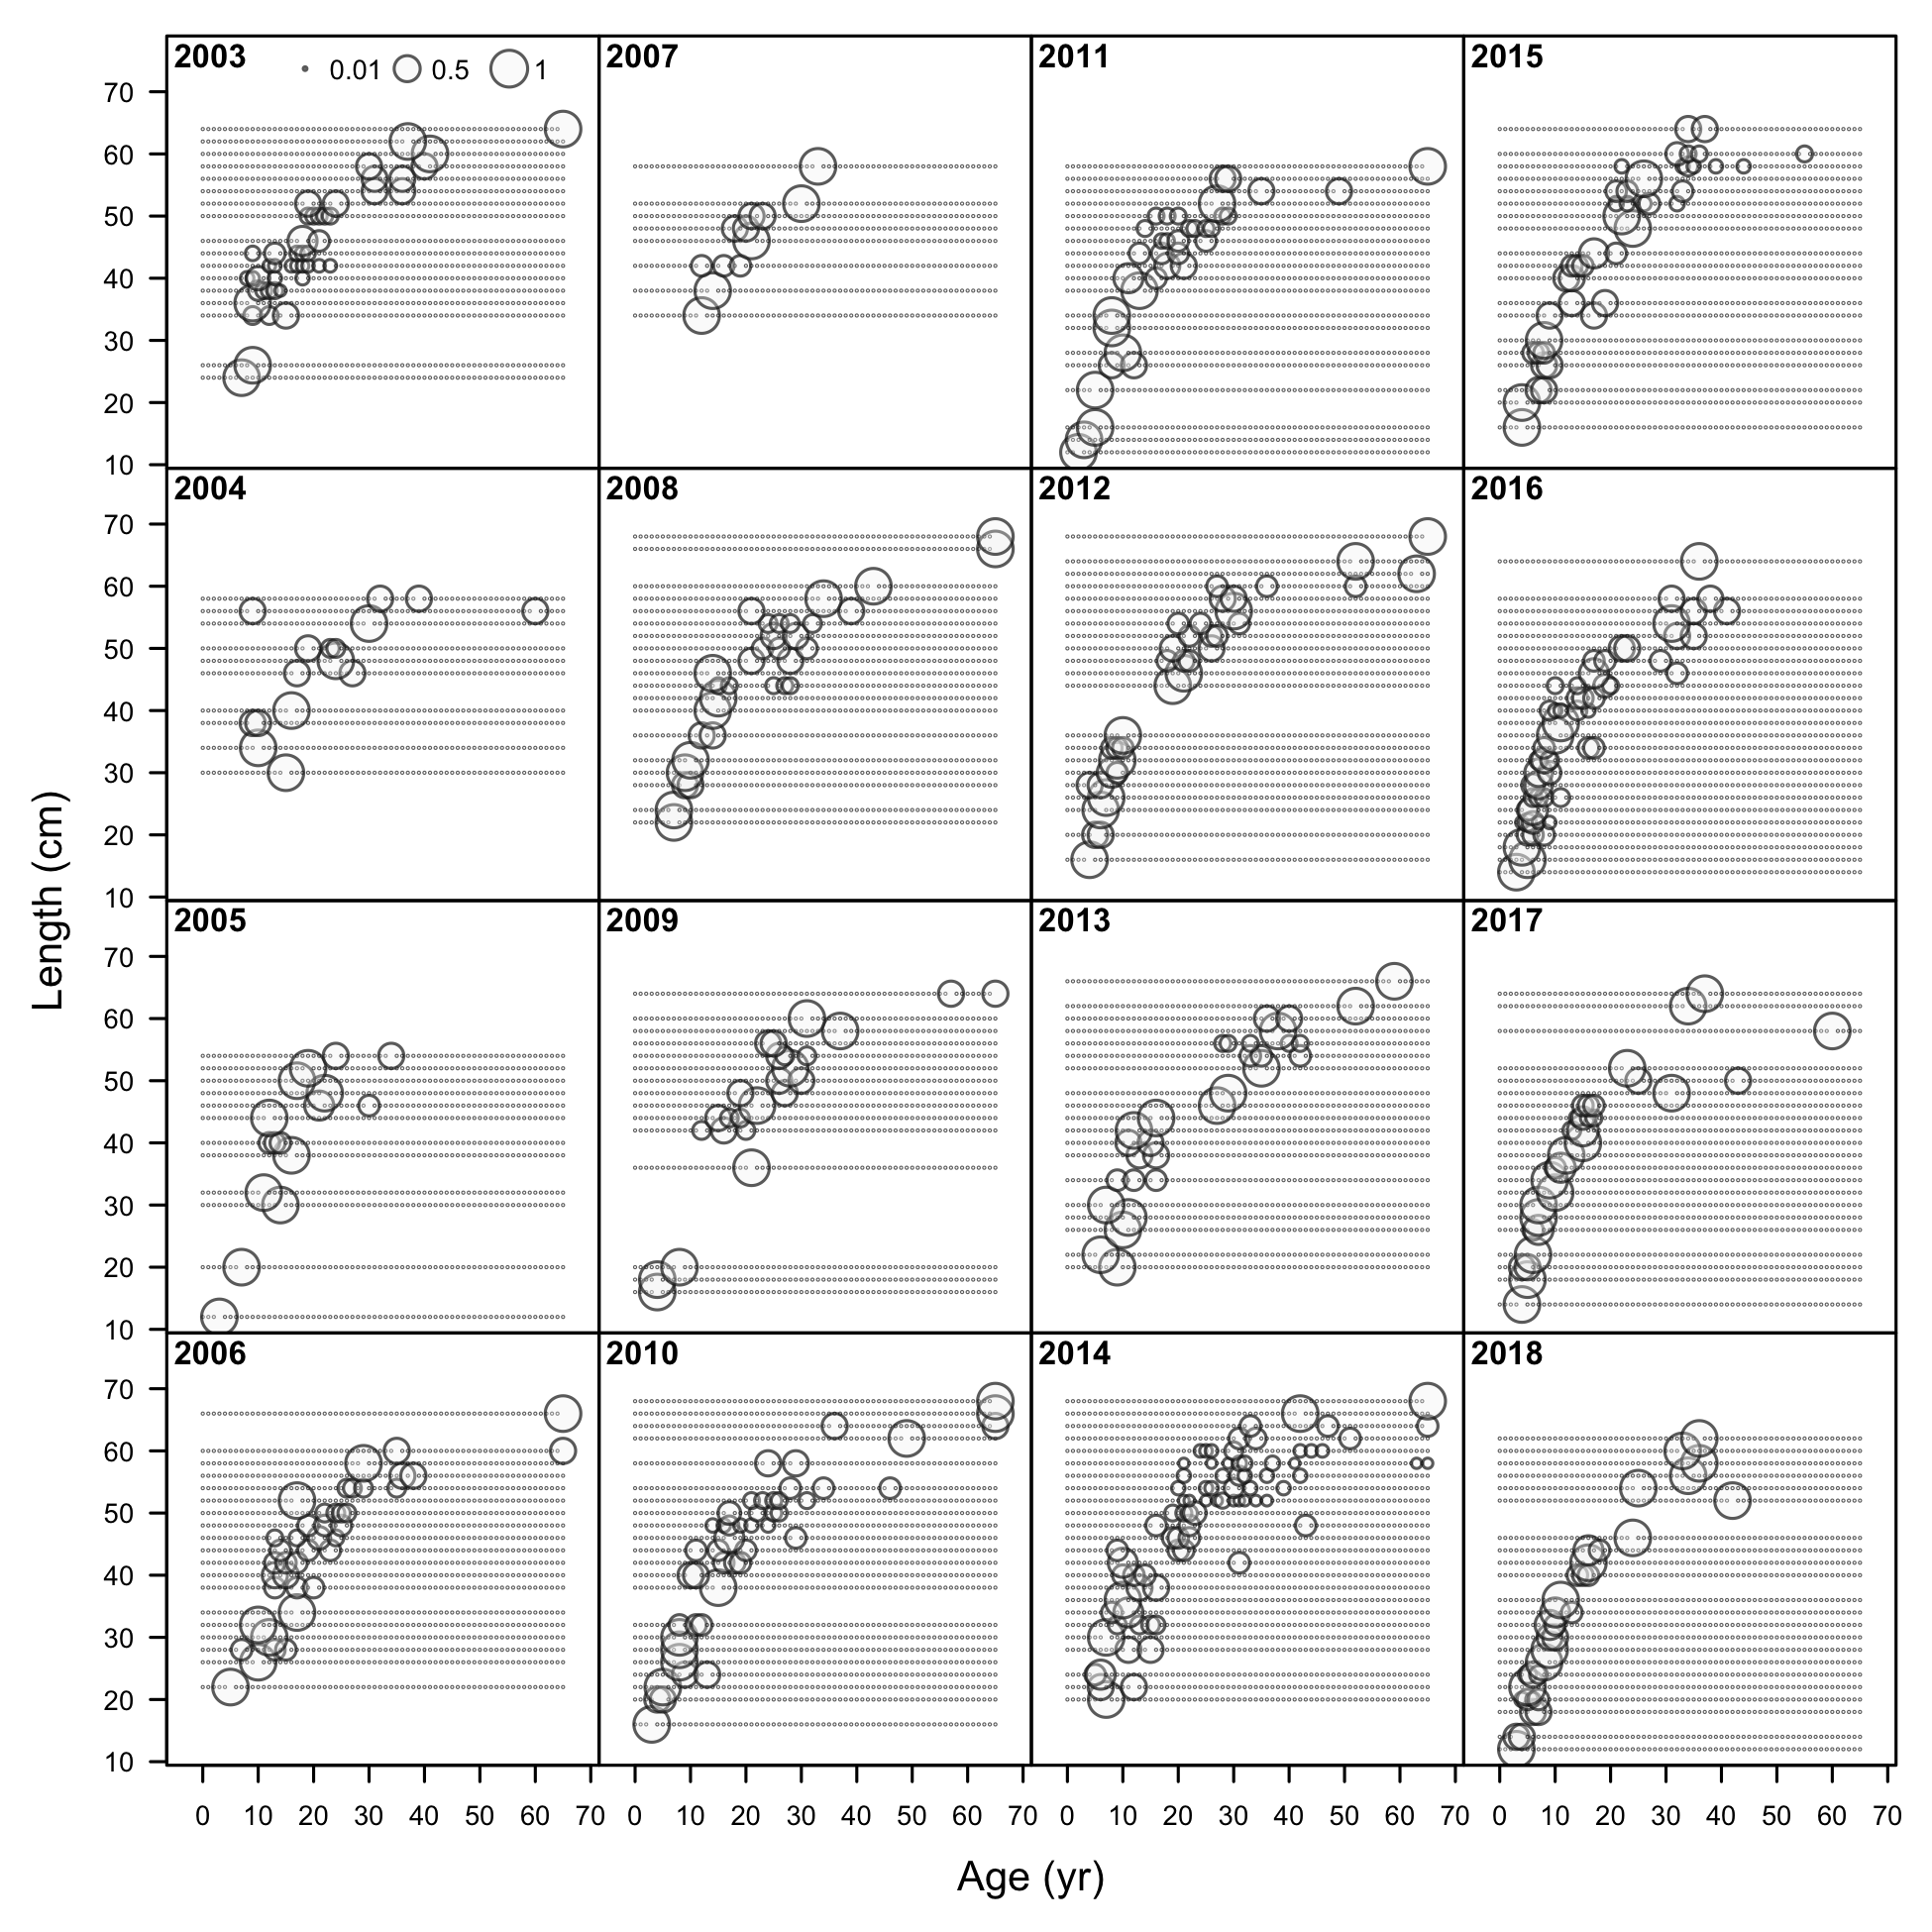
\includegraphics[width=6.5in,height=\textheight,keepaspectratio]{figures/r4ss_plots/plots/comp_condAALdat_bubflt11mkt0_page1.png}

}

\caption{\label{fig-NWFSC_agecomps1}Annual unsexed conditional
age-at-length data for the WCBTS (1 of 2).}

\end{figure}%

\begin{figure}

\centering{

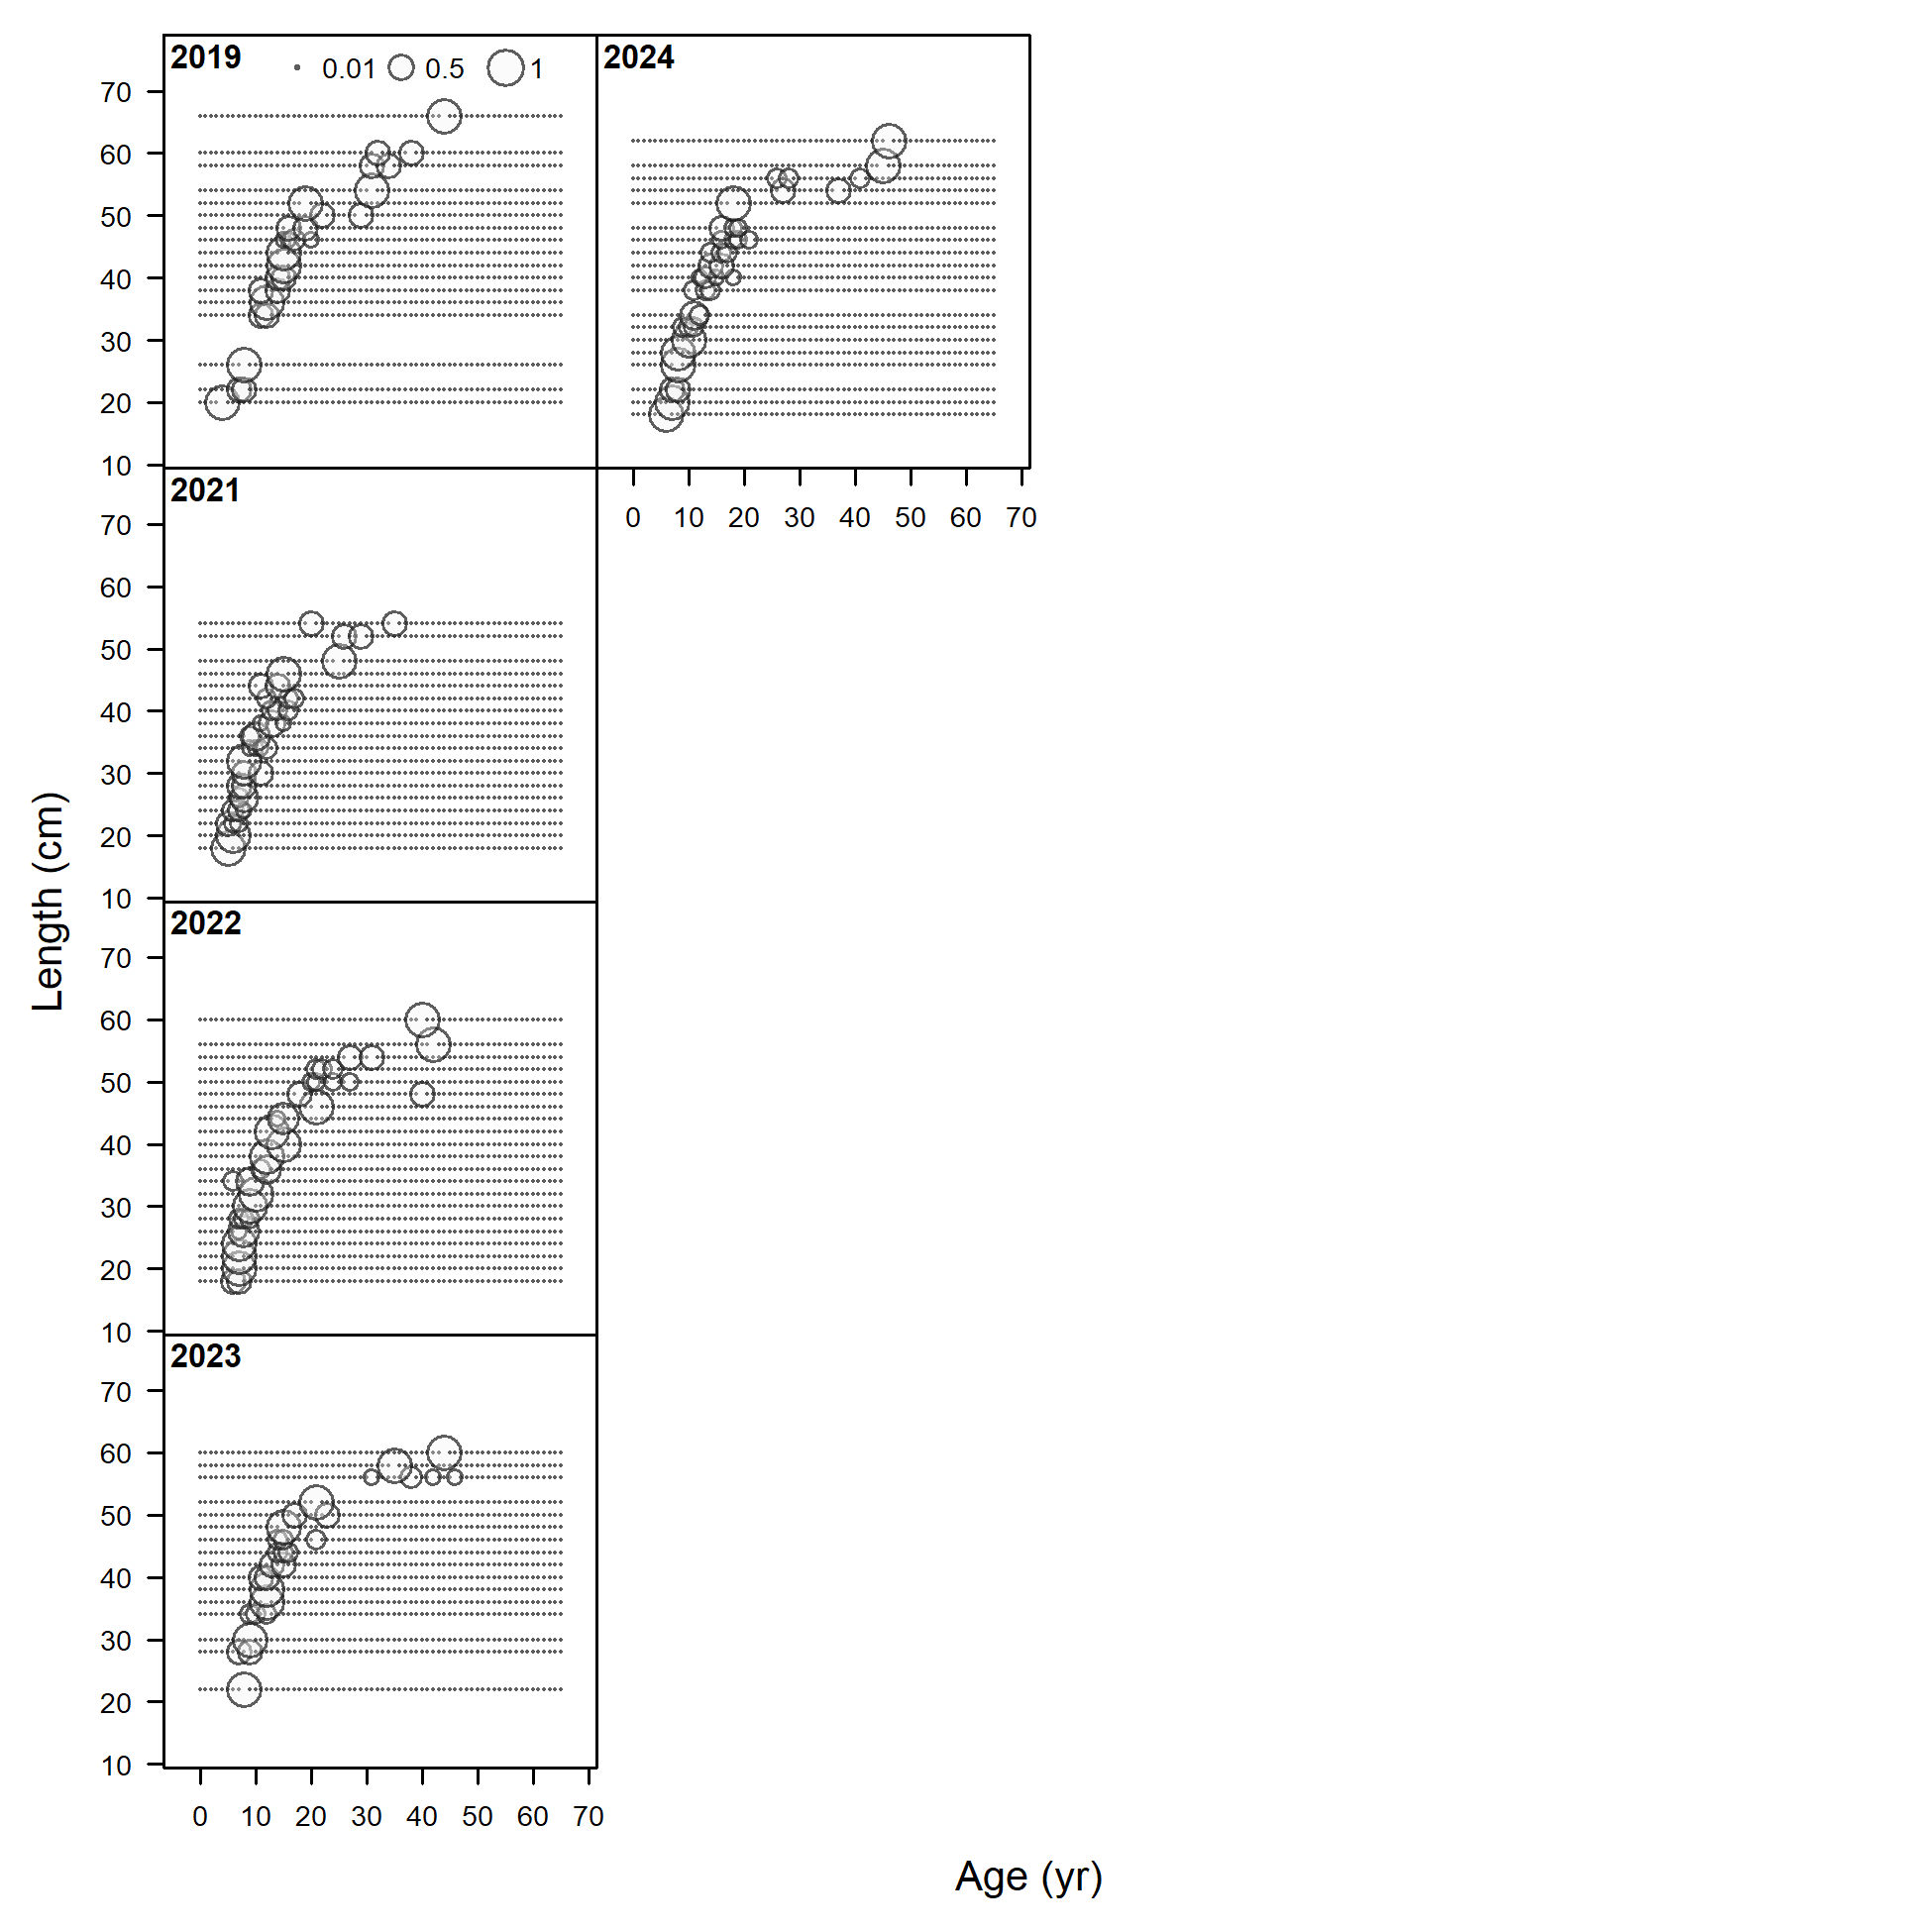
\includegraphics[width=6.5in,height=\textheight,keepaspectratio]{figures/r4ss_plots/plots/comp_condAALdat_bubflt11mkt0_page2.png}

}

\caption{\label{fig-NWFSC_agecomps2}Annual unsexed conditional
age-at-length data for the WCBTS (2 of 2).}

\end{figure}%

\begin{figure}

\centering{

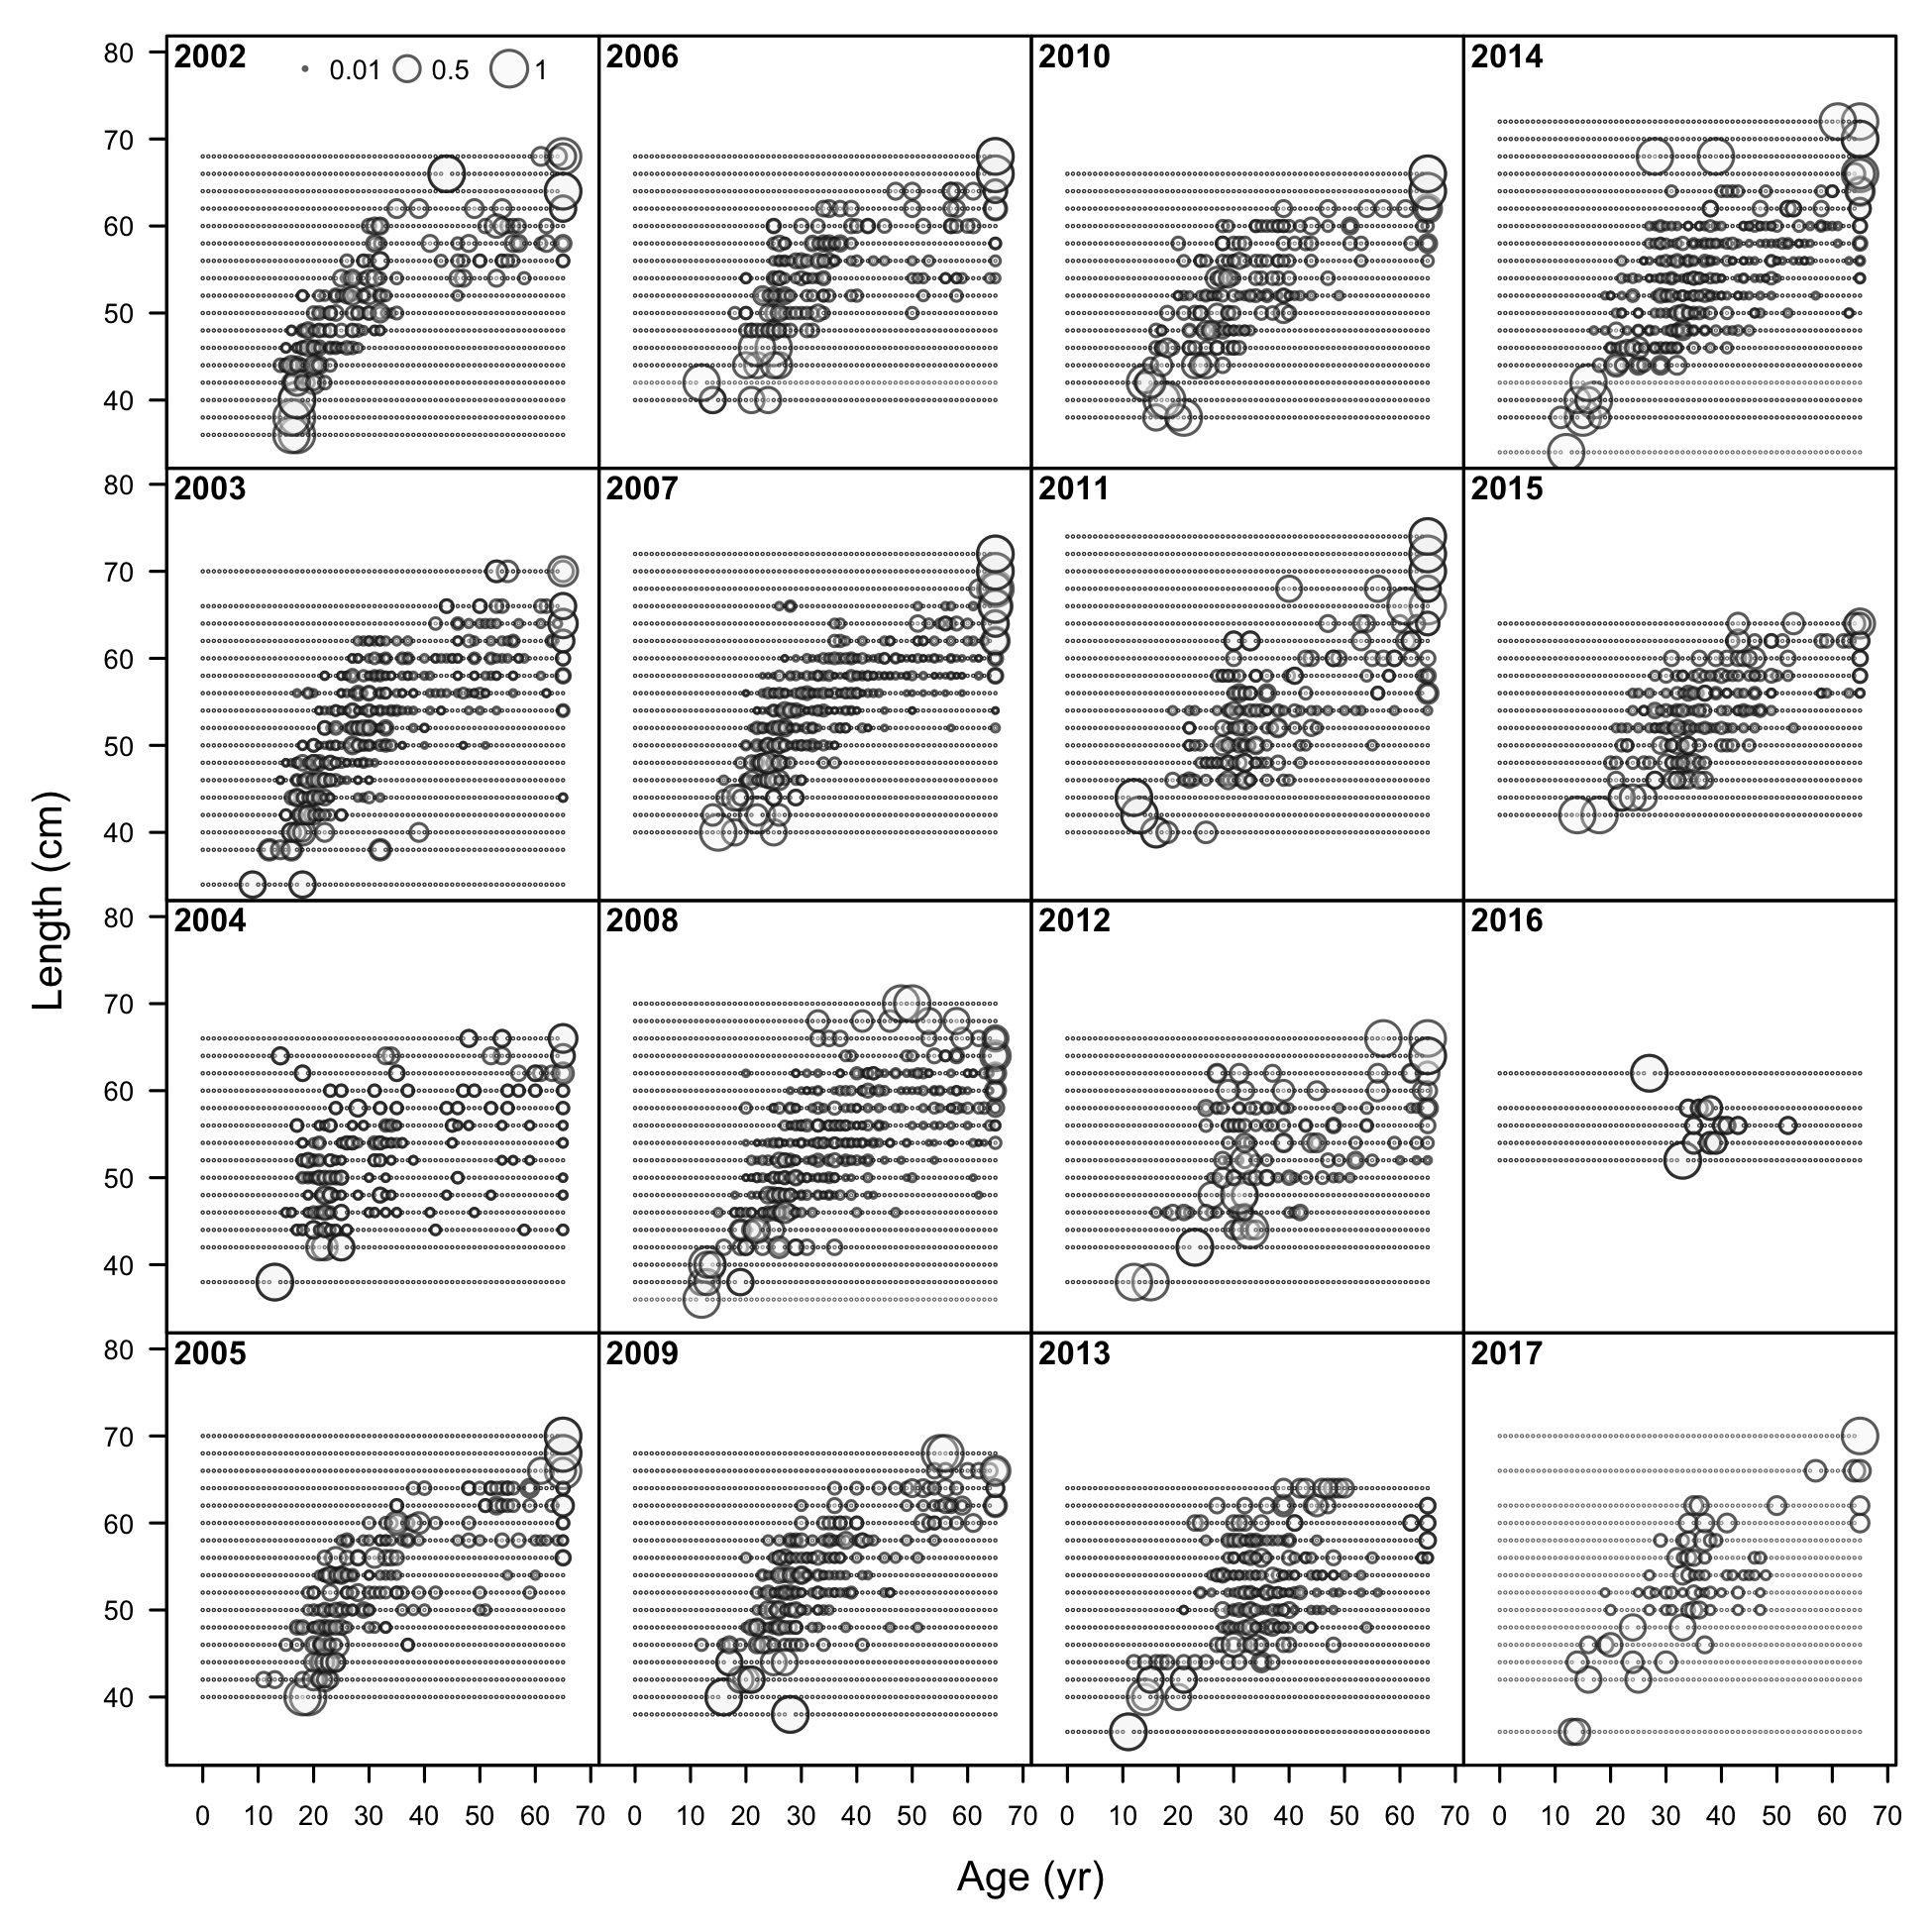
\includegraphics[width=6.5in,height=\textheight,keepaspectratio]{figures/r4ss_plots/plots/comp_condAALdat_bubflt12mkt0_page1.png}

}

\caption{\label{fig-IPHC_agecomps1}Annual unsexed conditional
age-at-length data for the IPHC (1 of 2).}

\end{figure}%

\begin{figure}

\centering{

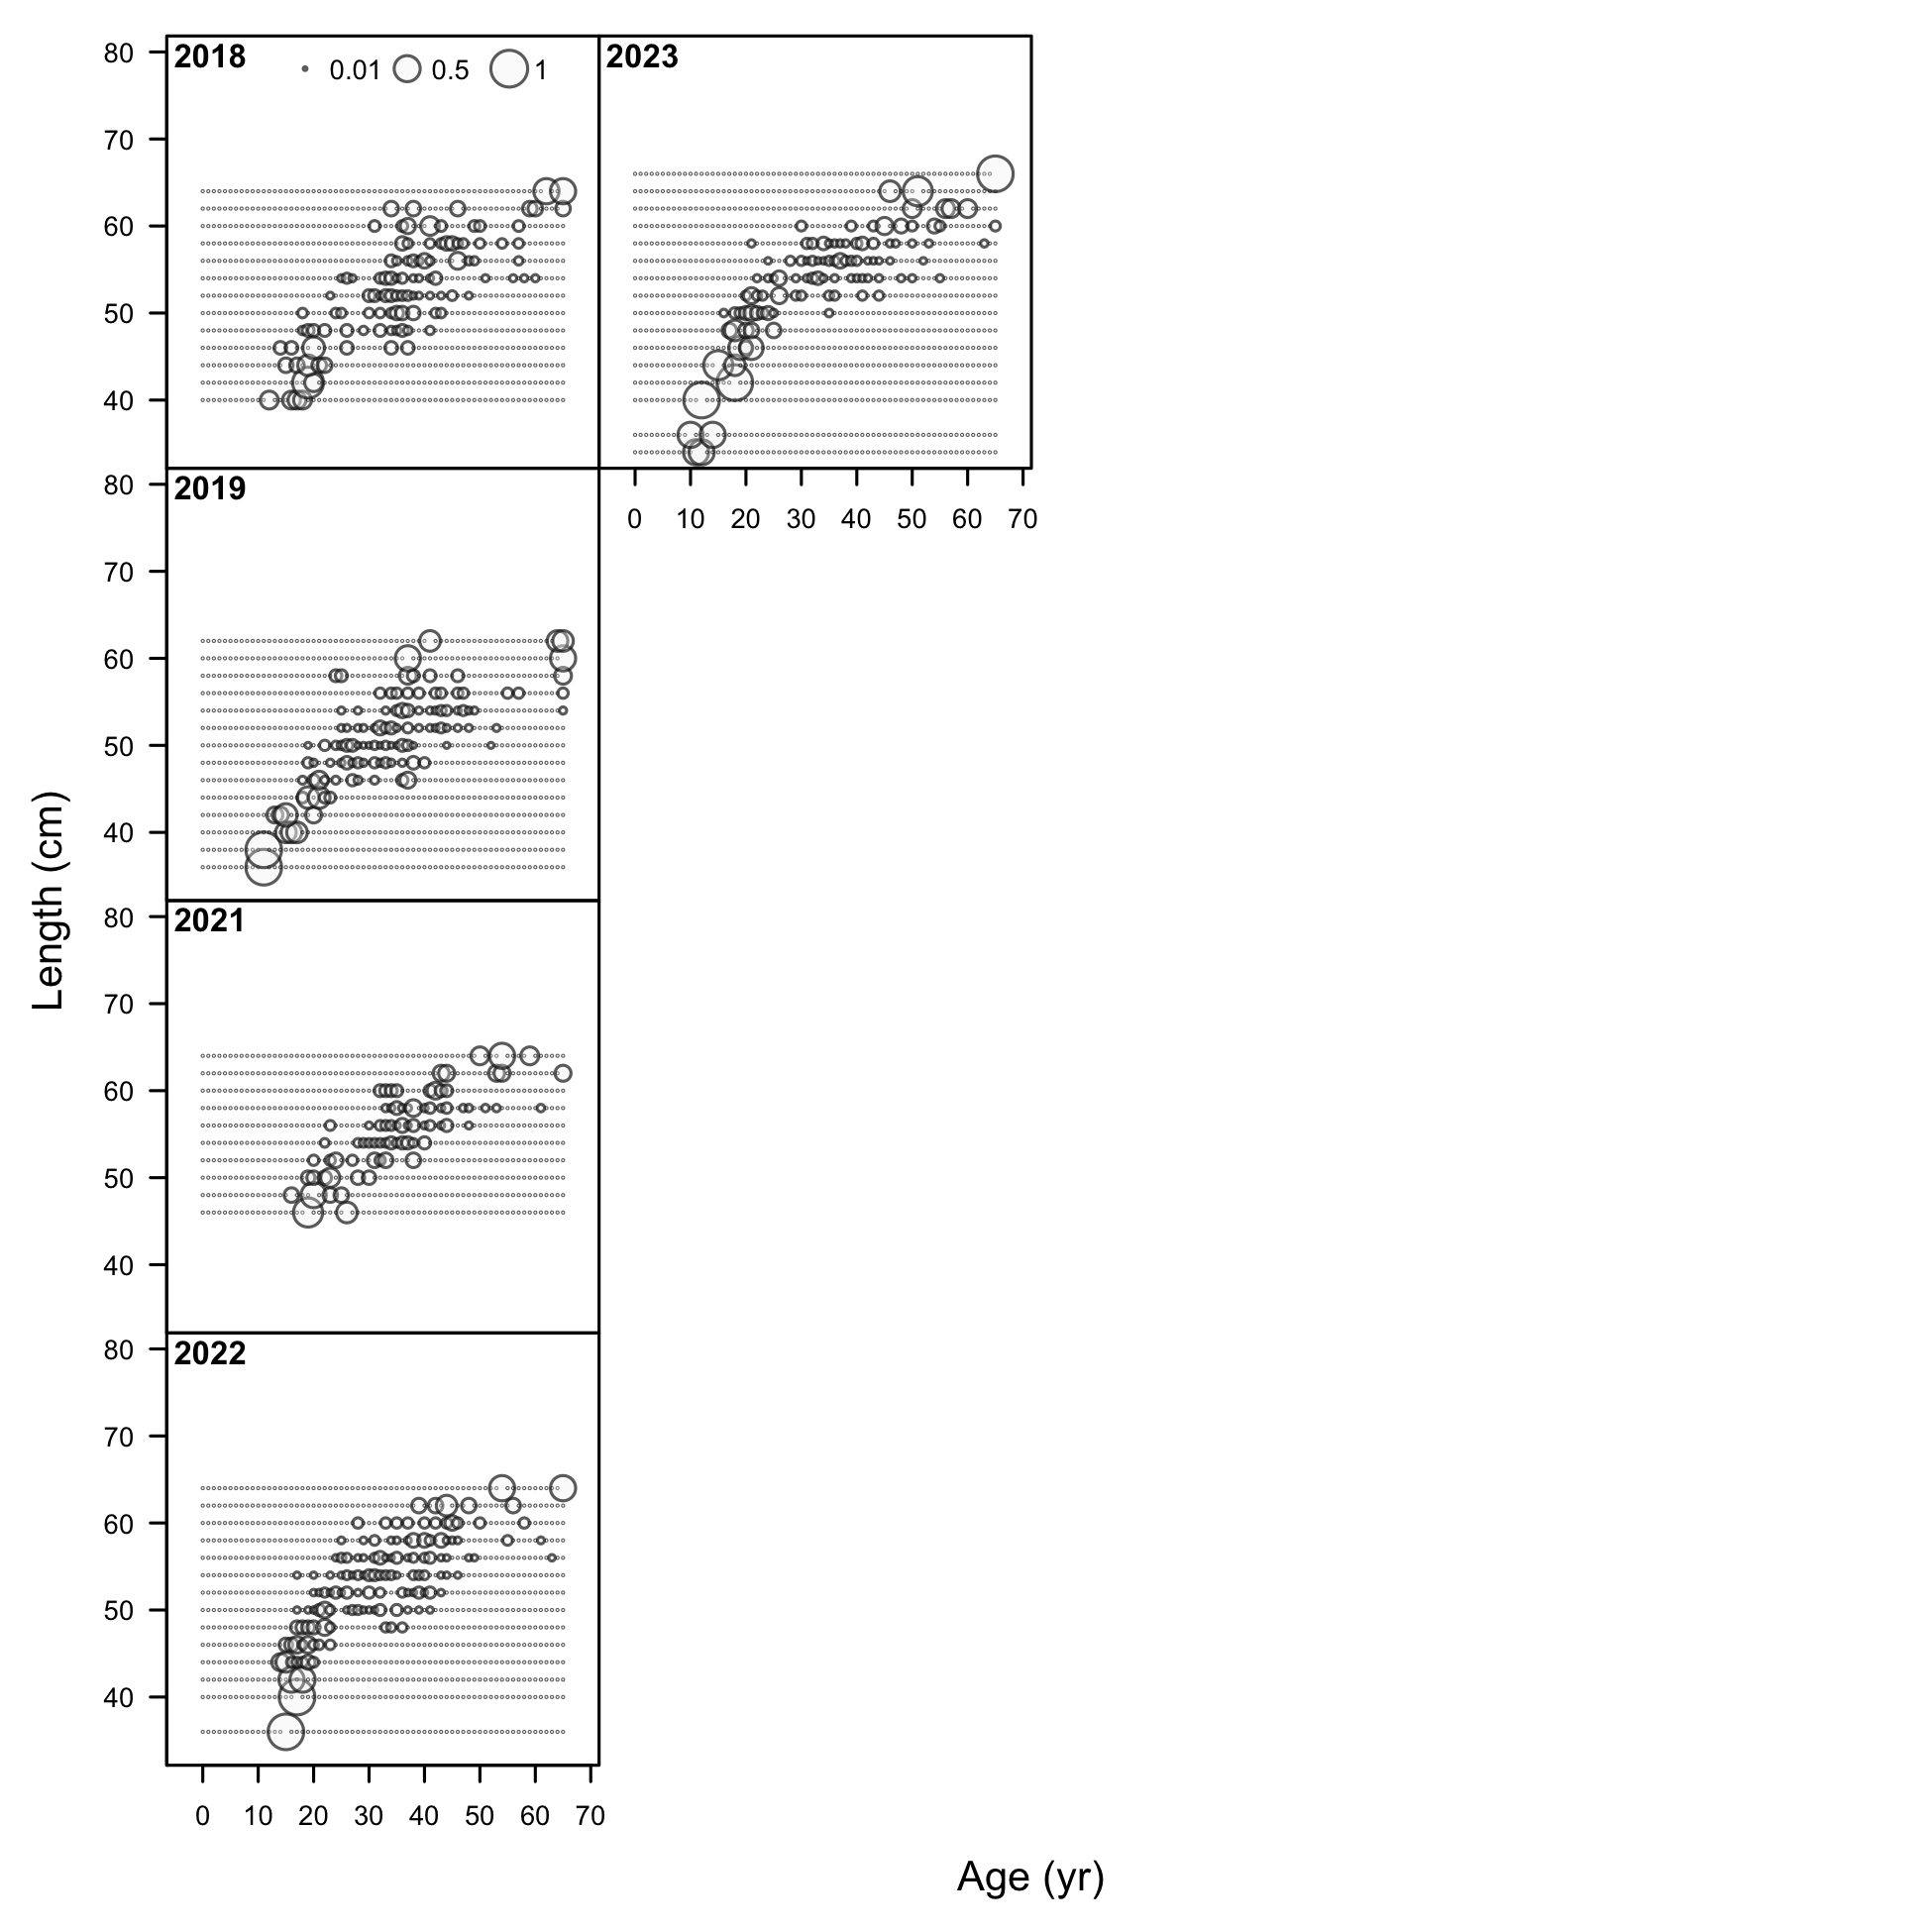
\includegraphics[width=6.5in,height=\textheight,keepaspectratio]{figures/r4ss_plots/plots/comp_condAALdat_bubflt12mkt0_page2.png}

}

\caption{\label{fig-IPHC_agecomps2}nnual unsexed conditional
age-at-length data for the IPHC (1 of 2).}

\end{figure}%

\begin{figure}

\centering{

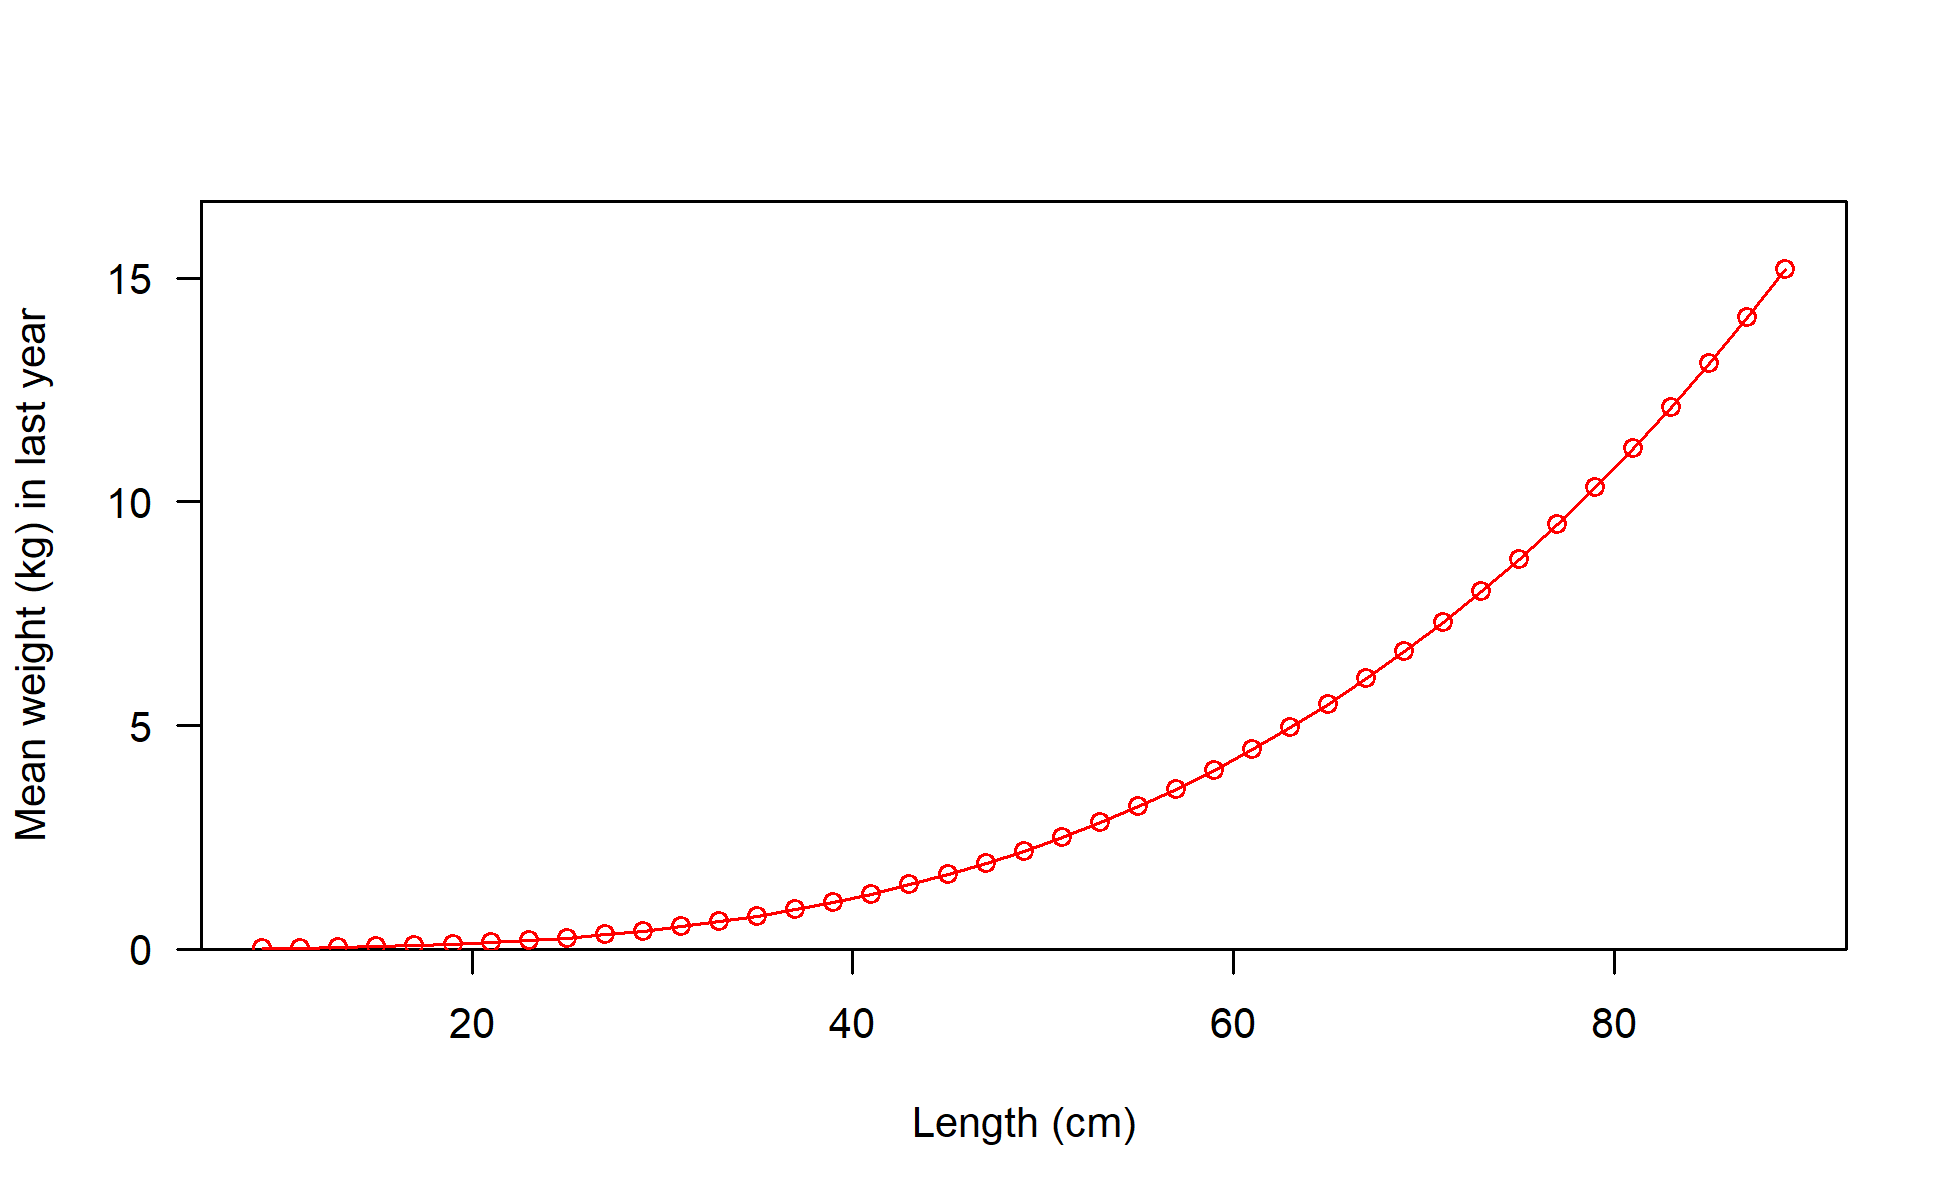
\includegraphics[width=6.5in,height=\textheight,keepaspectratio]{figures/r4ss_plots/plots/bio5_weightatsize.png}

}

\caption{\label{fig-LWrel}Updated weight-at-length relationship.}

\end{figure}%

\section{}\label{section}

\begin{figure}

\centering{

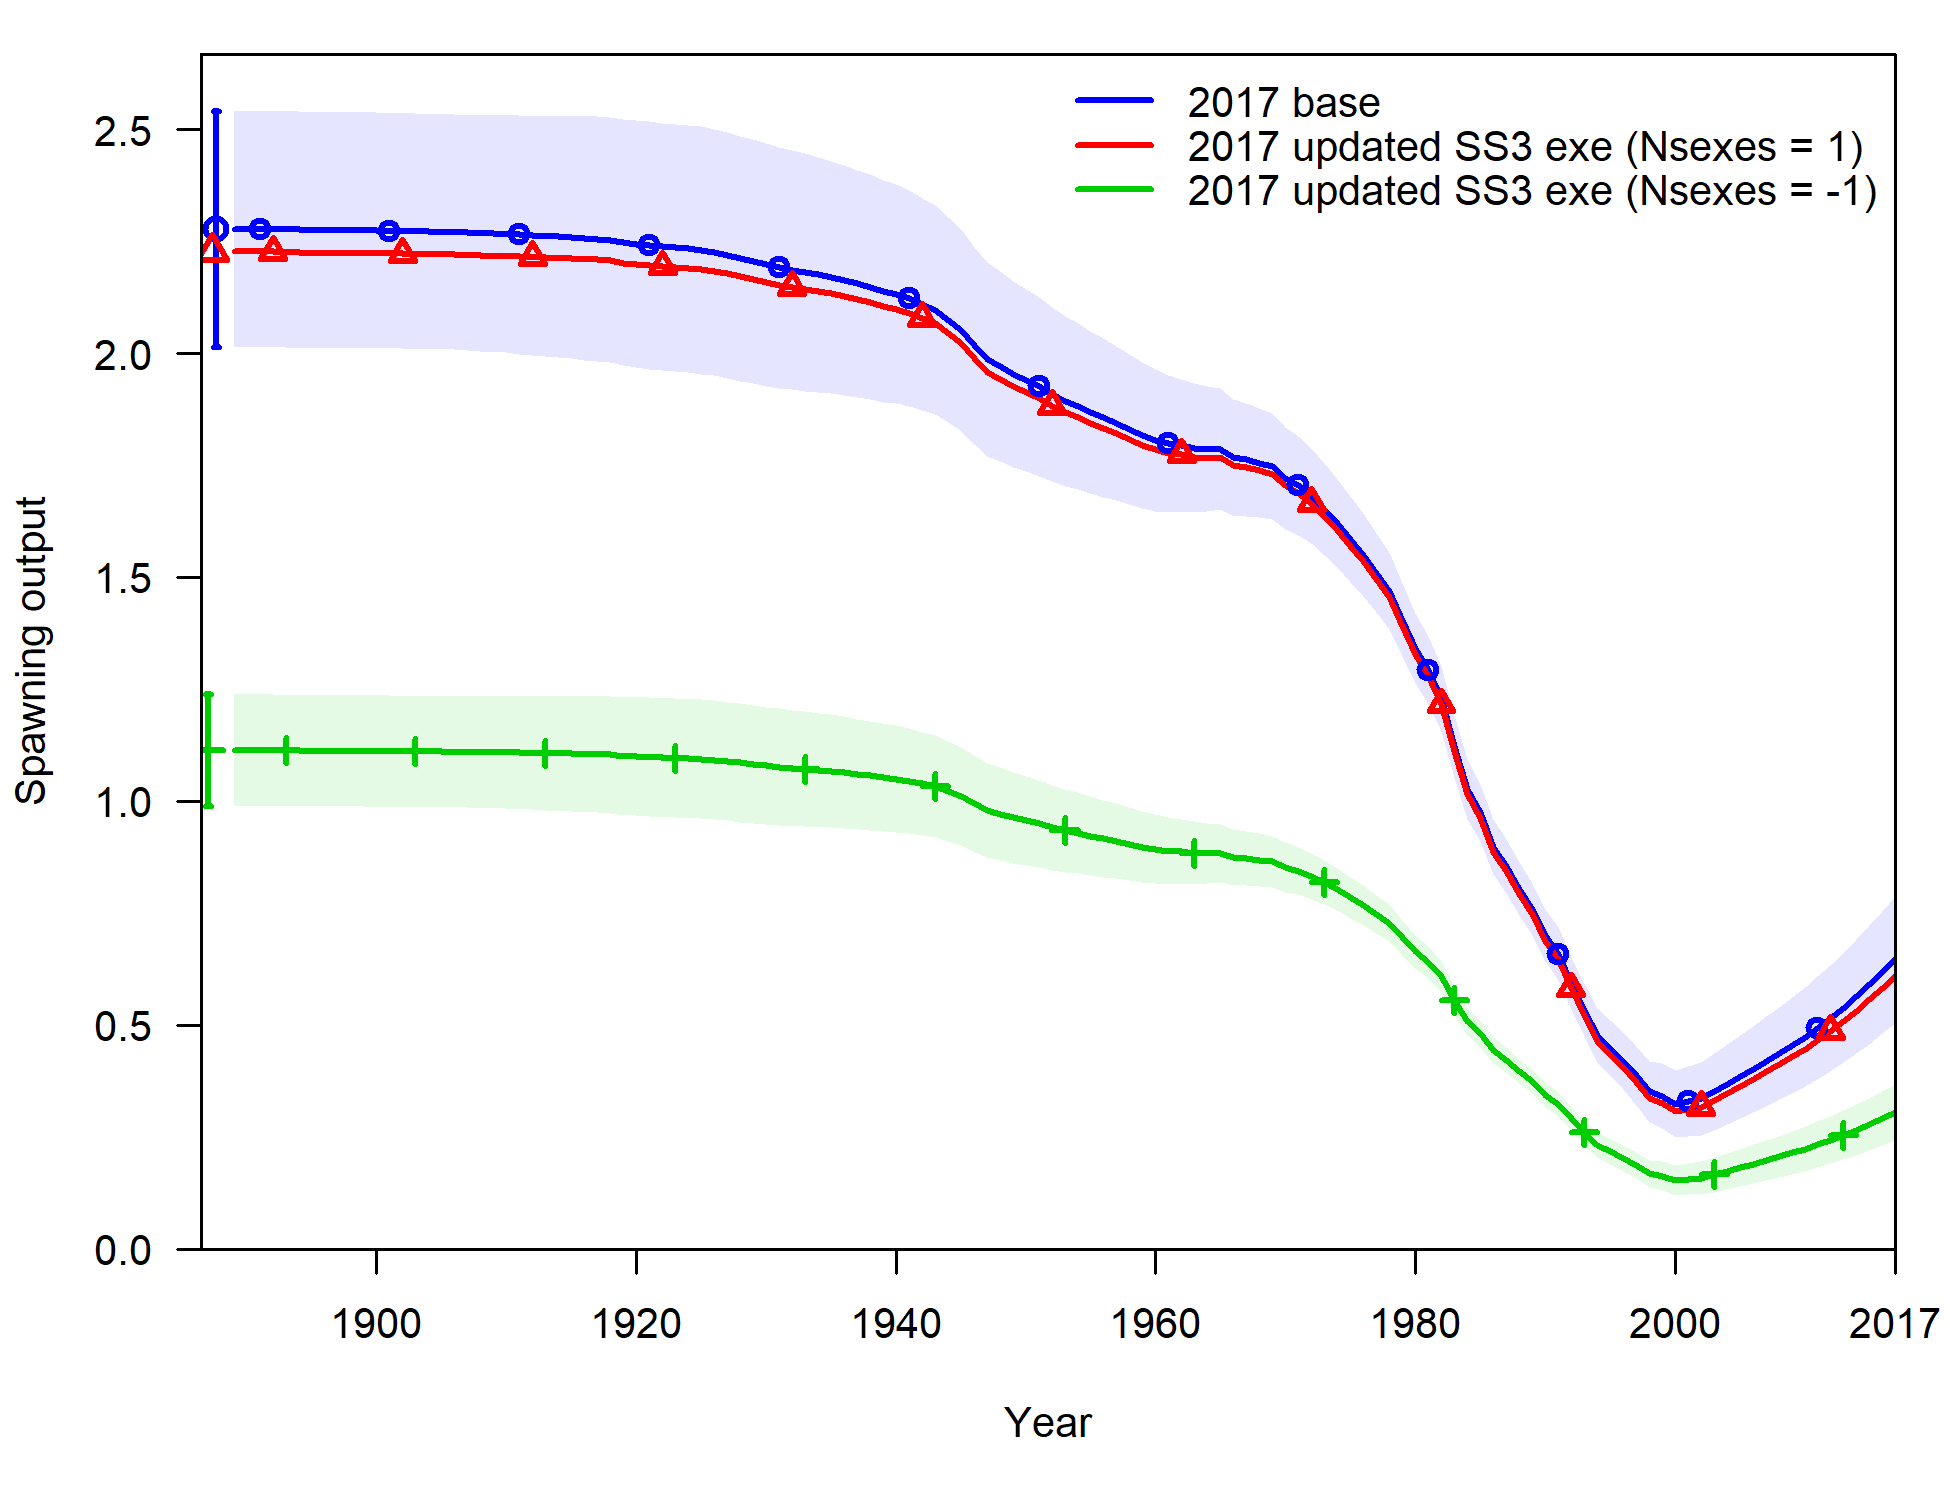
\includegraphics[width=6.5in,height=\textheight,keepaspectratio]{figures/bridging/1_SS3exe/compare2_spawnbio_uncertainty.png}

}

\caption{\label{fig-ss3exe_1}Comparison of the spawning output for the
2017 model with the updated SS3 executable and a single-sex model.}

\end{figure}%

\begin{figure}

\centering{

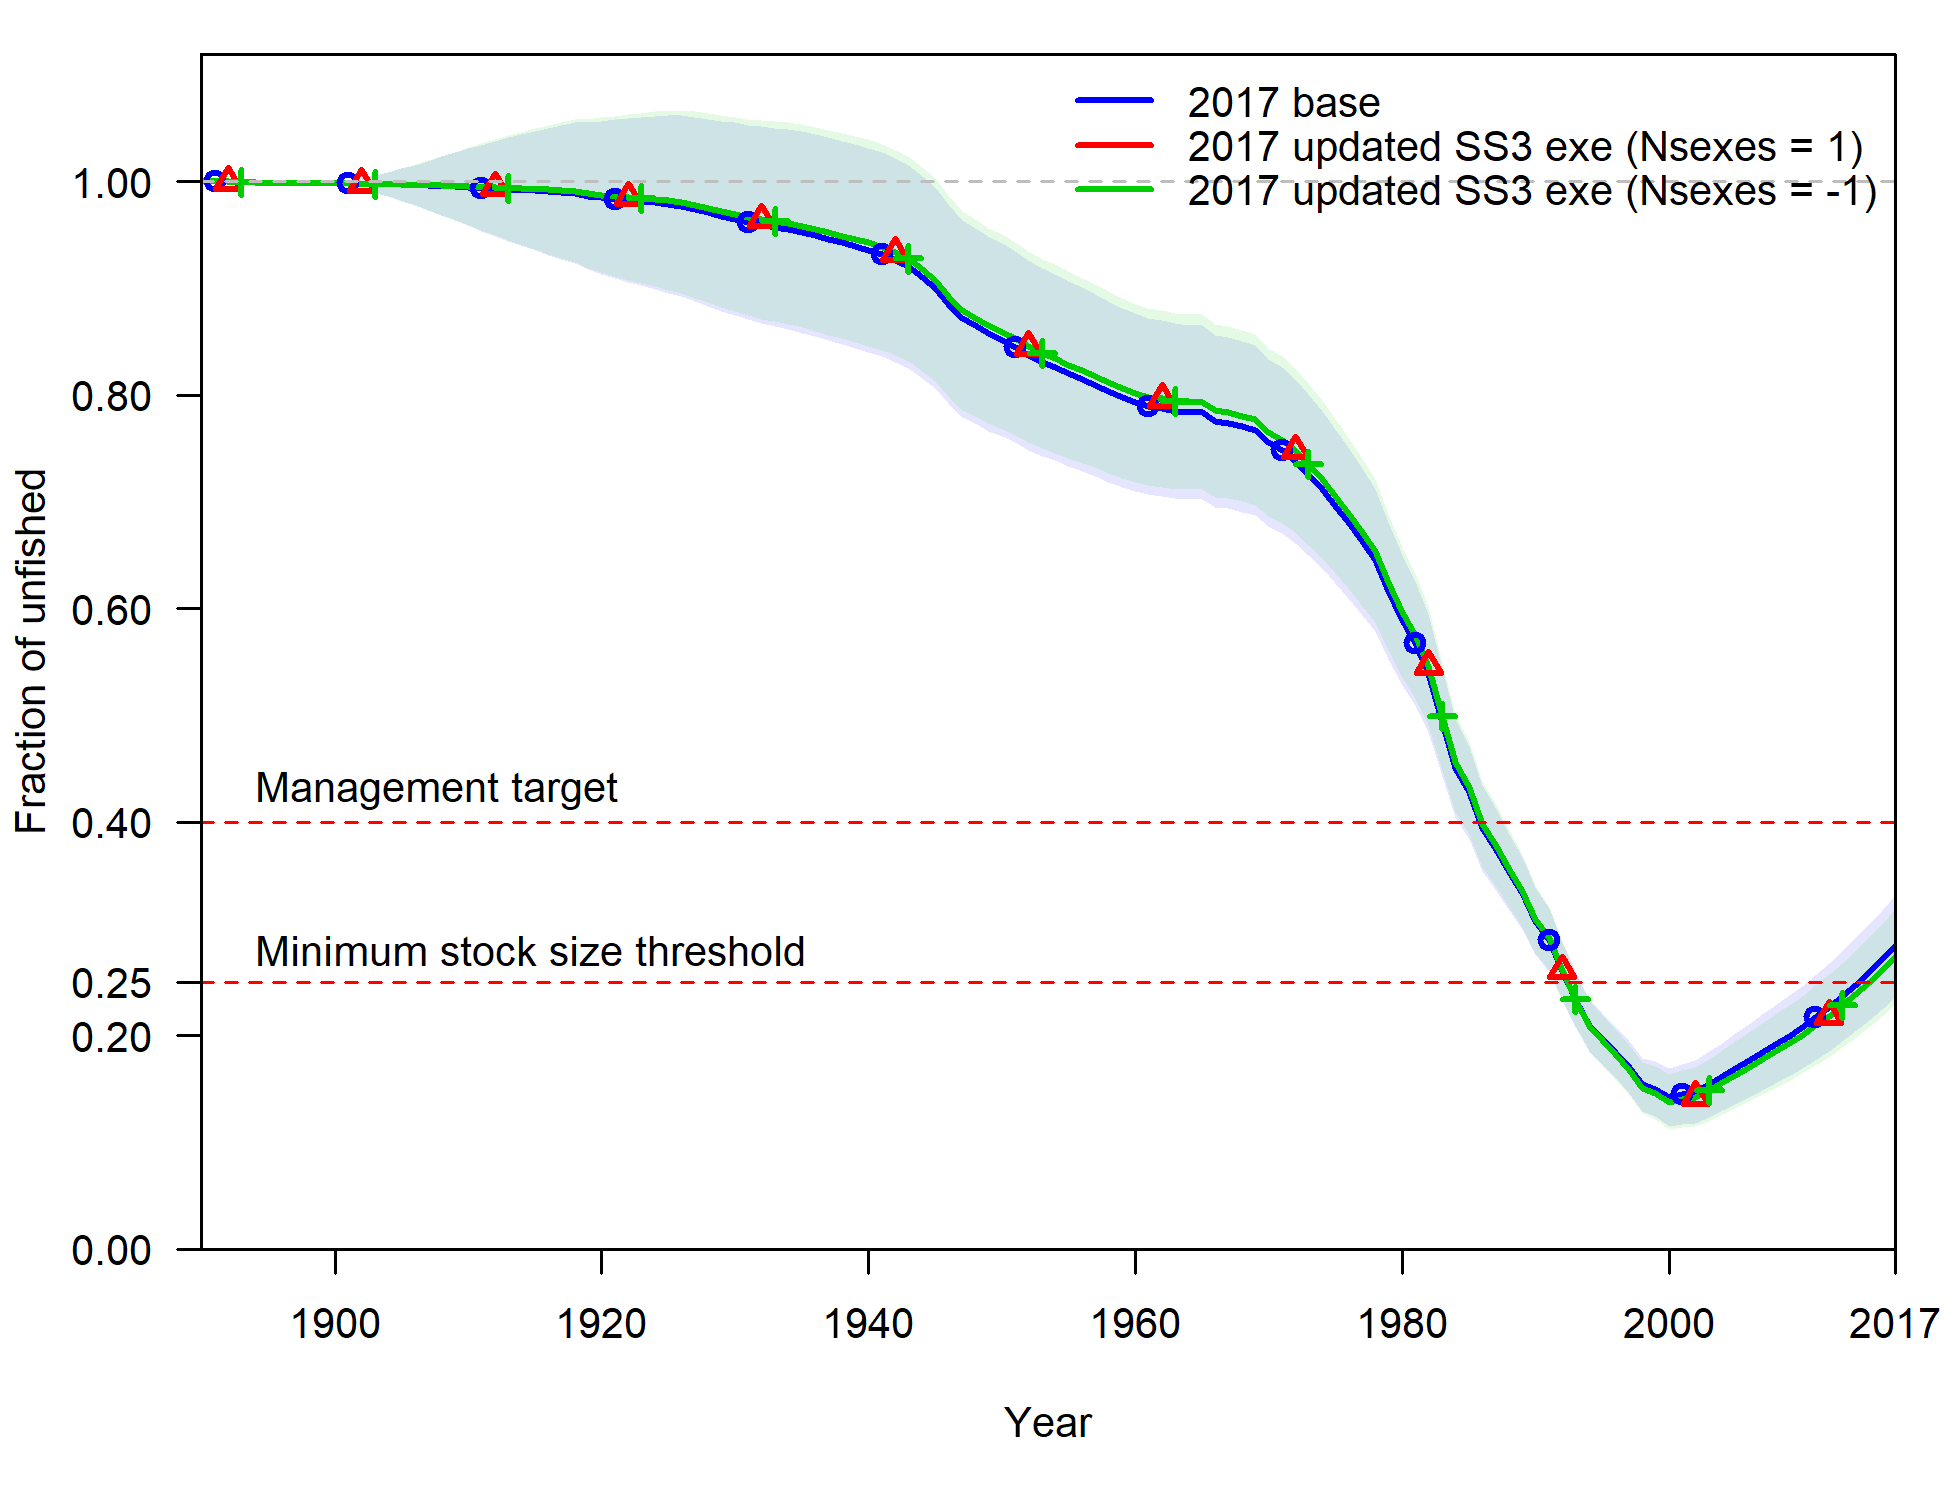
\includegraphics[width=6.5in,height=\textheight,keepaspectratio]{figures/bridging/1_SS3exe/compare4_Bratio_uncertainty.png}

}

\caption{\label{fig-ss3exe_2}Comparison of the stock status for the 2017
model with the updated SS3 executable and a single-sex model.}

\end{figure}%

\clearpage

\begin{figure}

\centering{

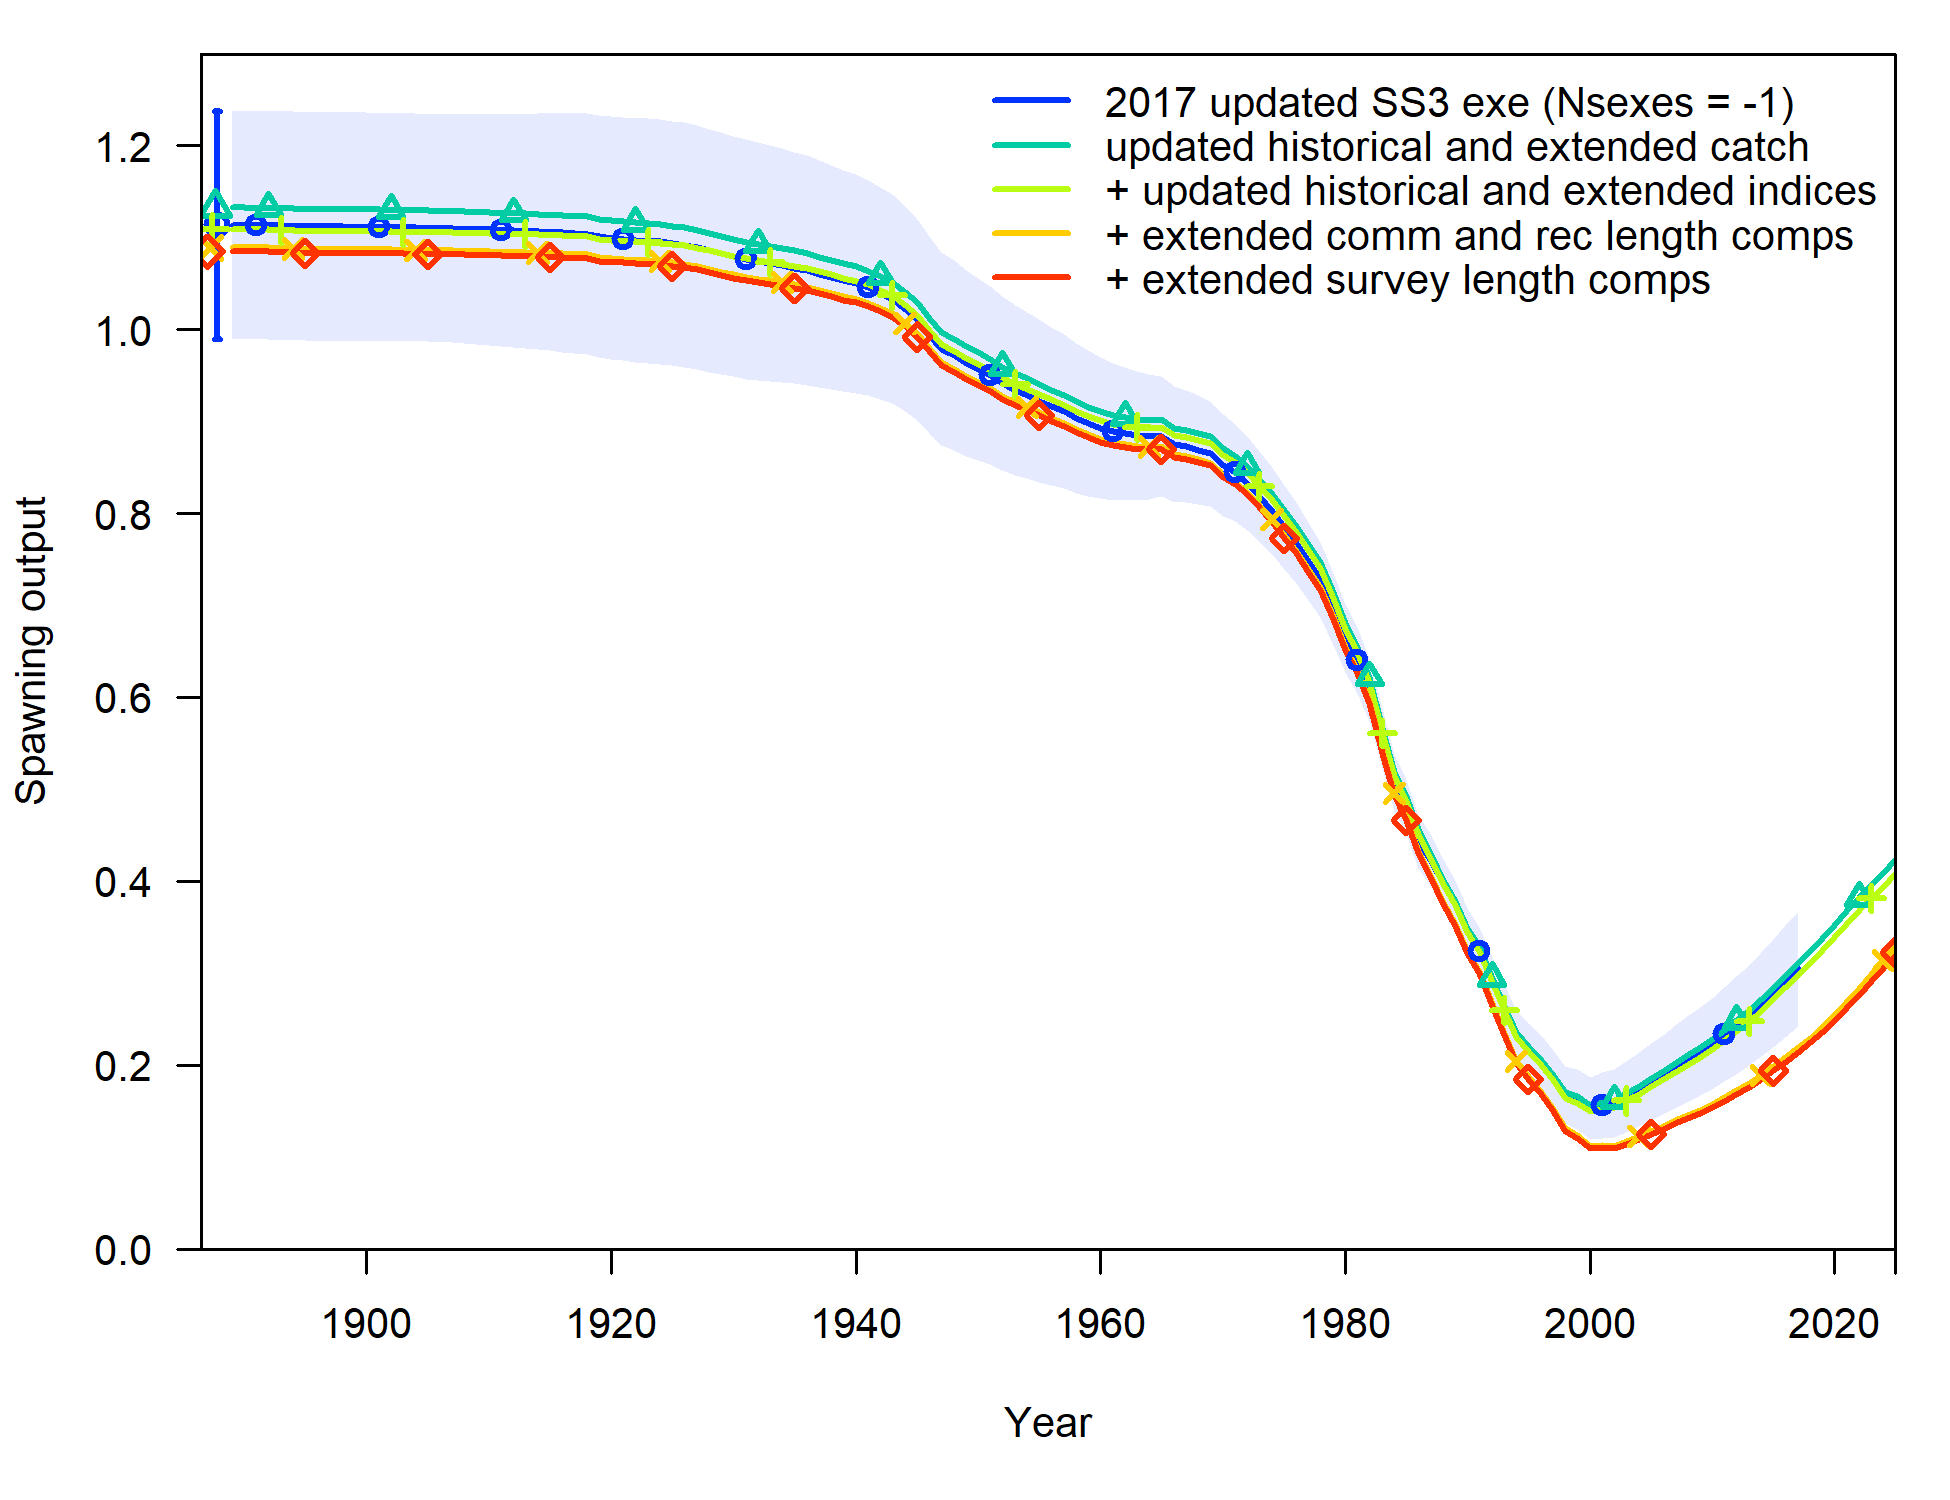
\includegraphics[width=6.5in,height=\textheight,keepaspectratio]{figures/bridging/8_newlencomps/compare2_spawnbio_uncertainty.png}

}

\caption{\label{fig-newdata_1}Comparison of the spawning output of the
2017 model with an updated SS3 executable (blue), updated catch data
(dark green), updated indices (light green), new fishery length
composition data (orange), and survey length composition data (red).}

\end{figure}%

\begin{figure}

\centering{

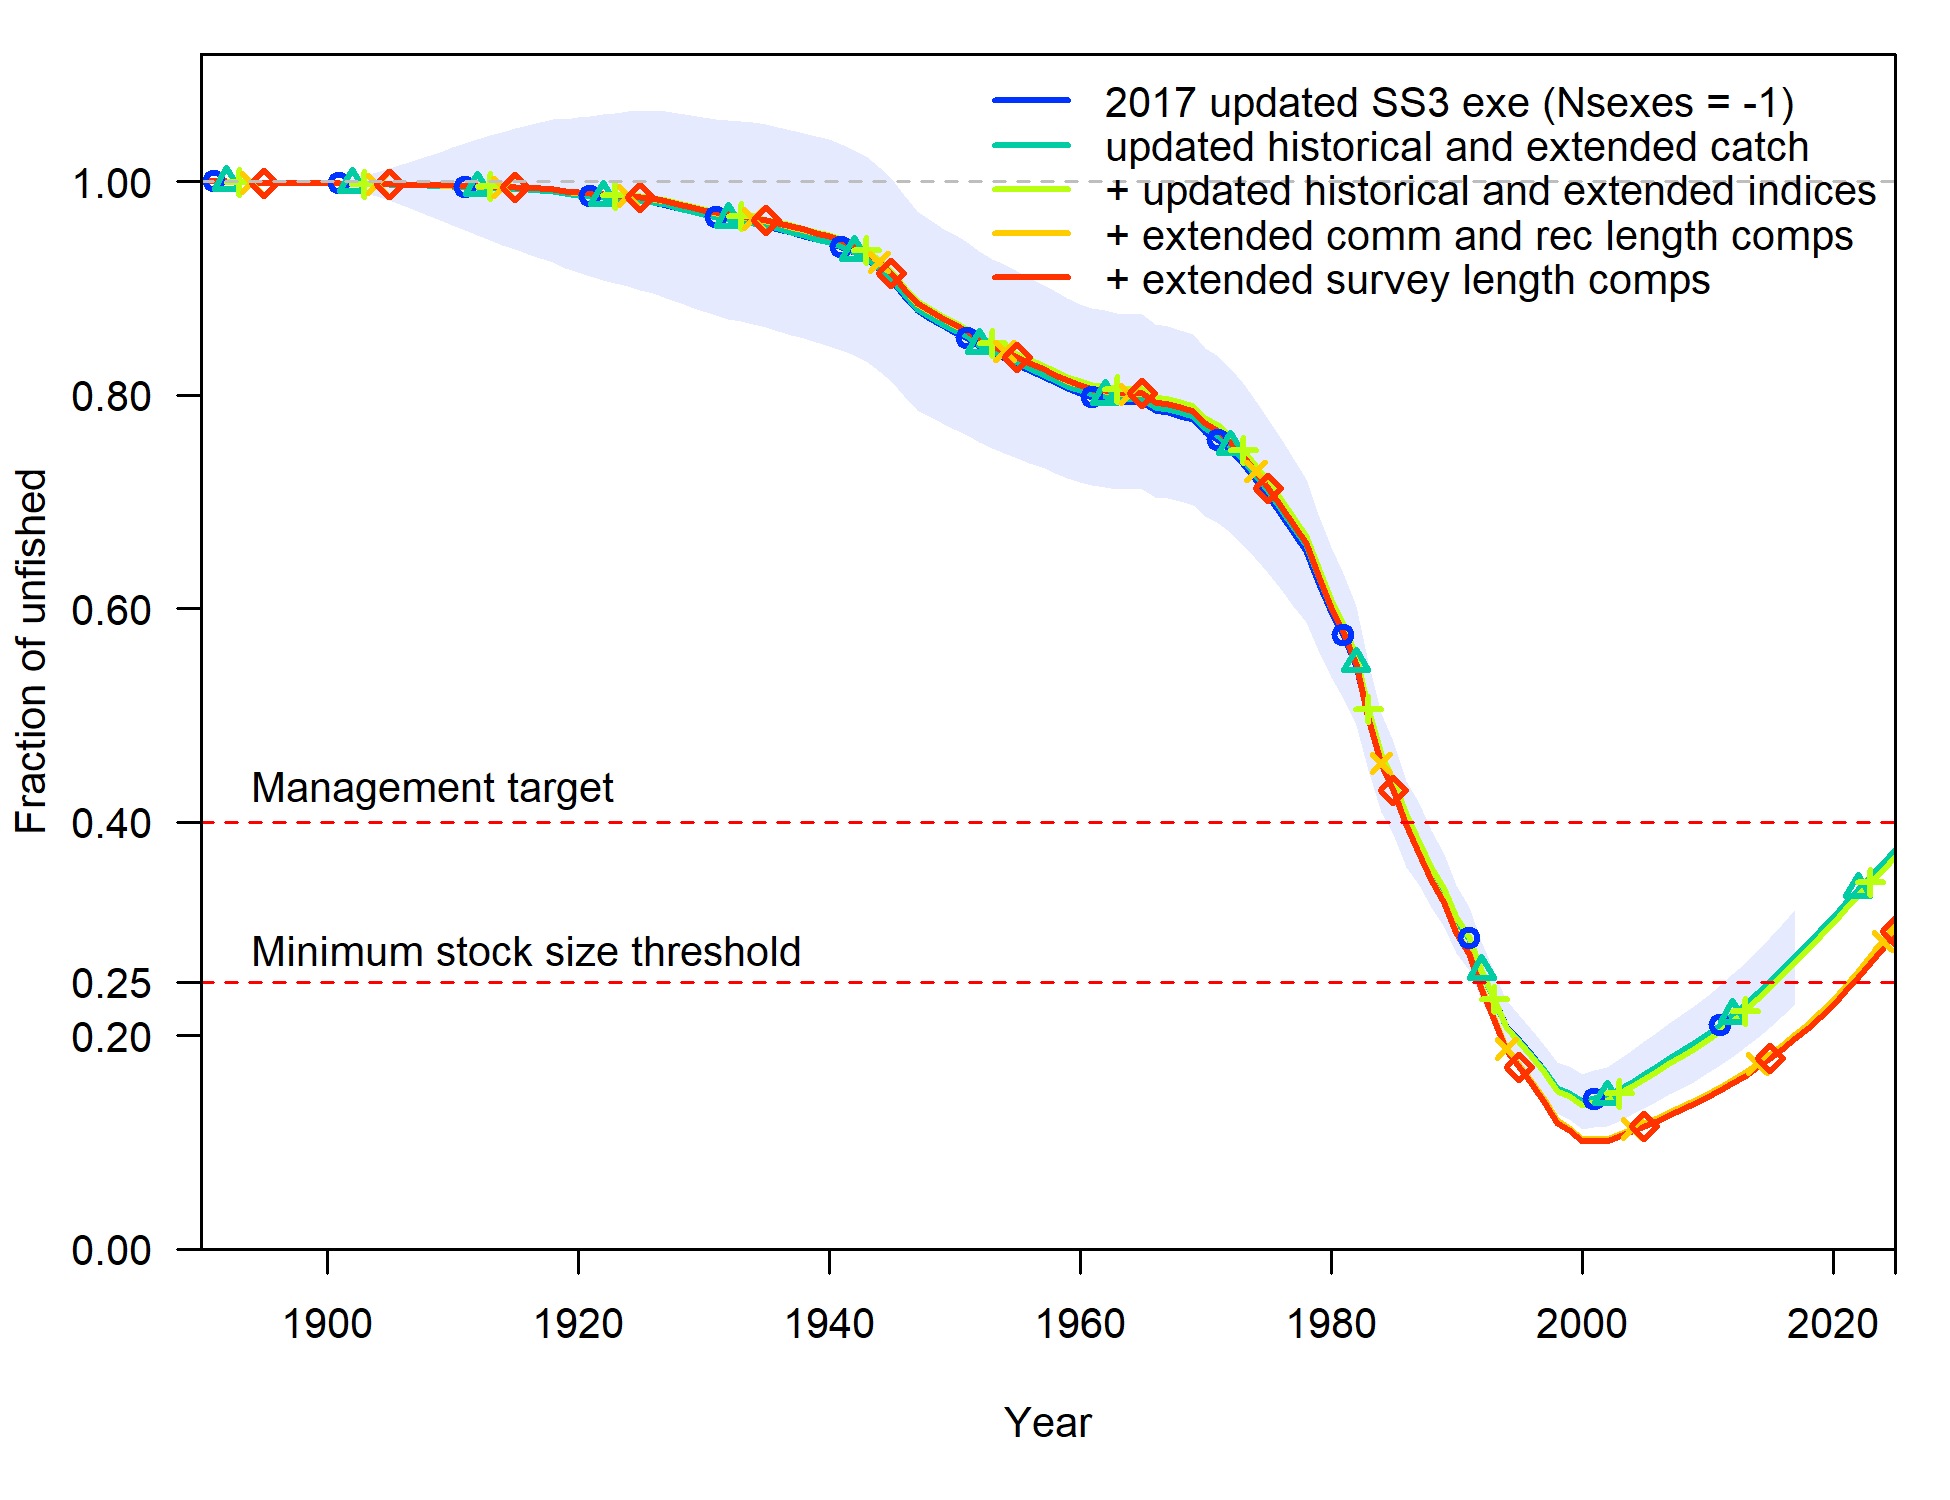
\includegraphics[width=6.5in,height=\textheight,keepaspectratio]{figures/bridging/8_newlencomps/compare4_Bratio_uncertainty.png}

}

\caption{\label{fig-newdata_2}Comparison of the stock status of the 2017
model with an updated SS3 executable (blue), updated catch data (dark
green), updated indices (light green), new fishery length composition
data (orange), and survey length composition data (red).}

\end{figure}%

\begin{figure}

\centering{

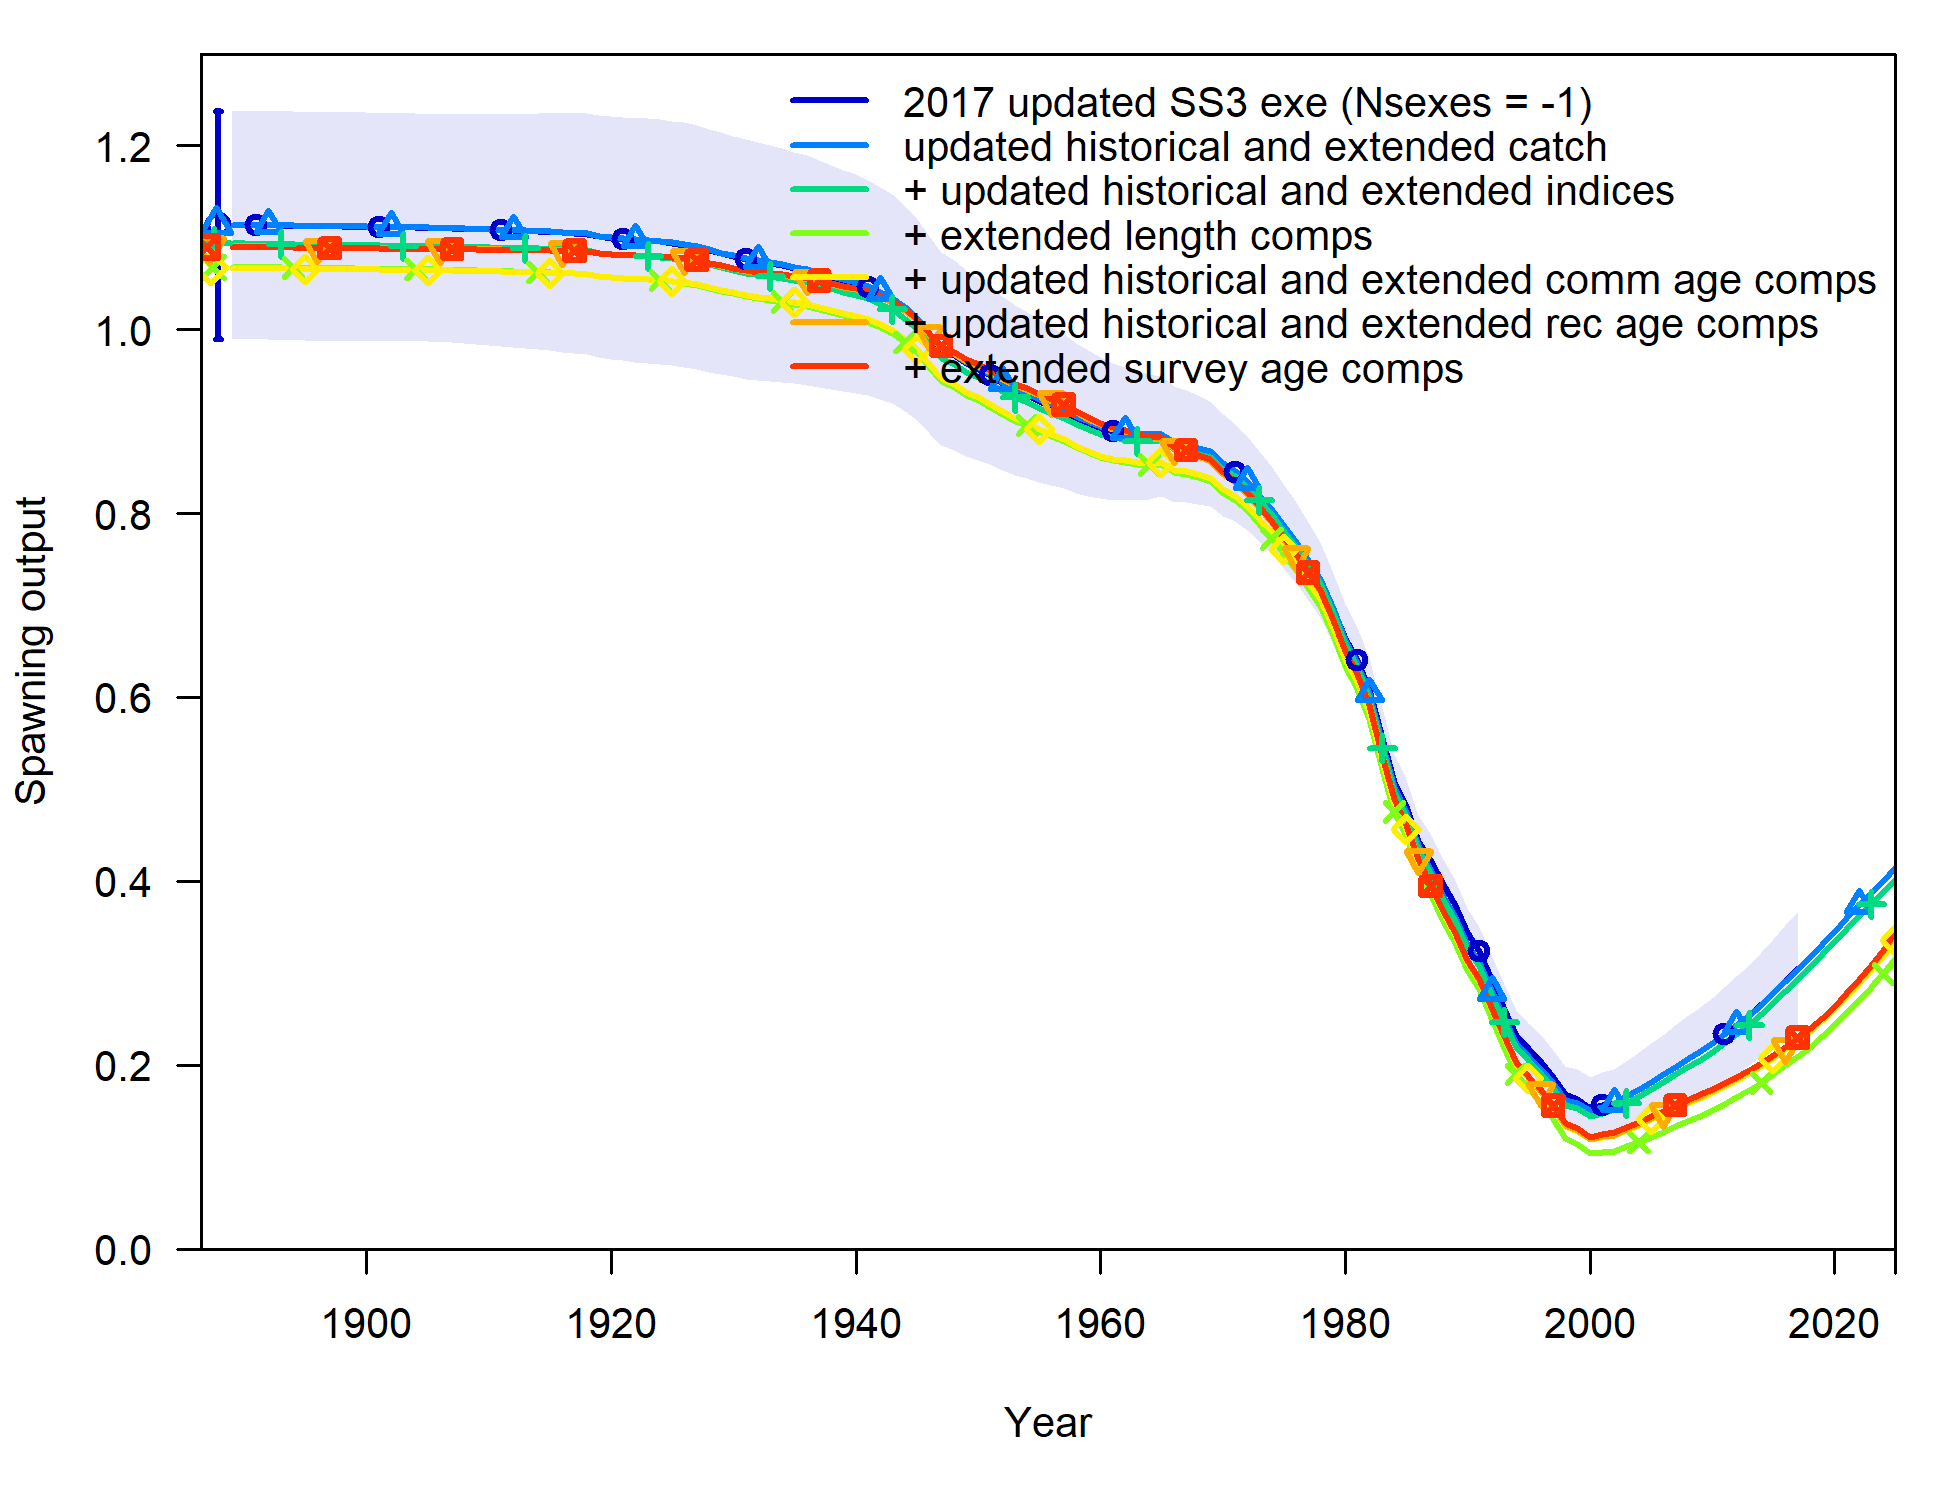
\includegraphics[width=6.5in,height=\textheight,keepaspectratio]{figures/bridging/13_newagecomps/compare2_spawnbio_uncertainty.png}

}

\caption{\label{fig-newdata_3}Comparison of the spawning output of the
2017 model with an updated SS3 executable (blue), updated catch data
(light blue), updated indices (dark green), new fishery length
composition data (light green), and commercial (yellow), recreational
(orange), and survey (red) age composition data.}

\end{figure}%

\begin{figure}

\centering{

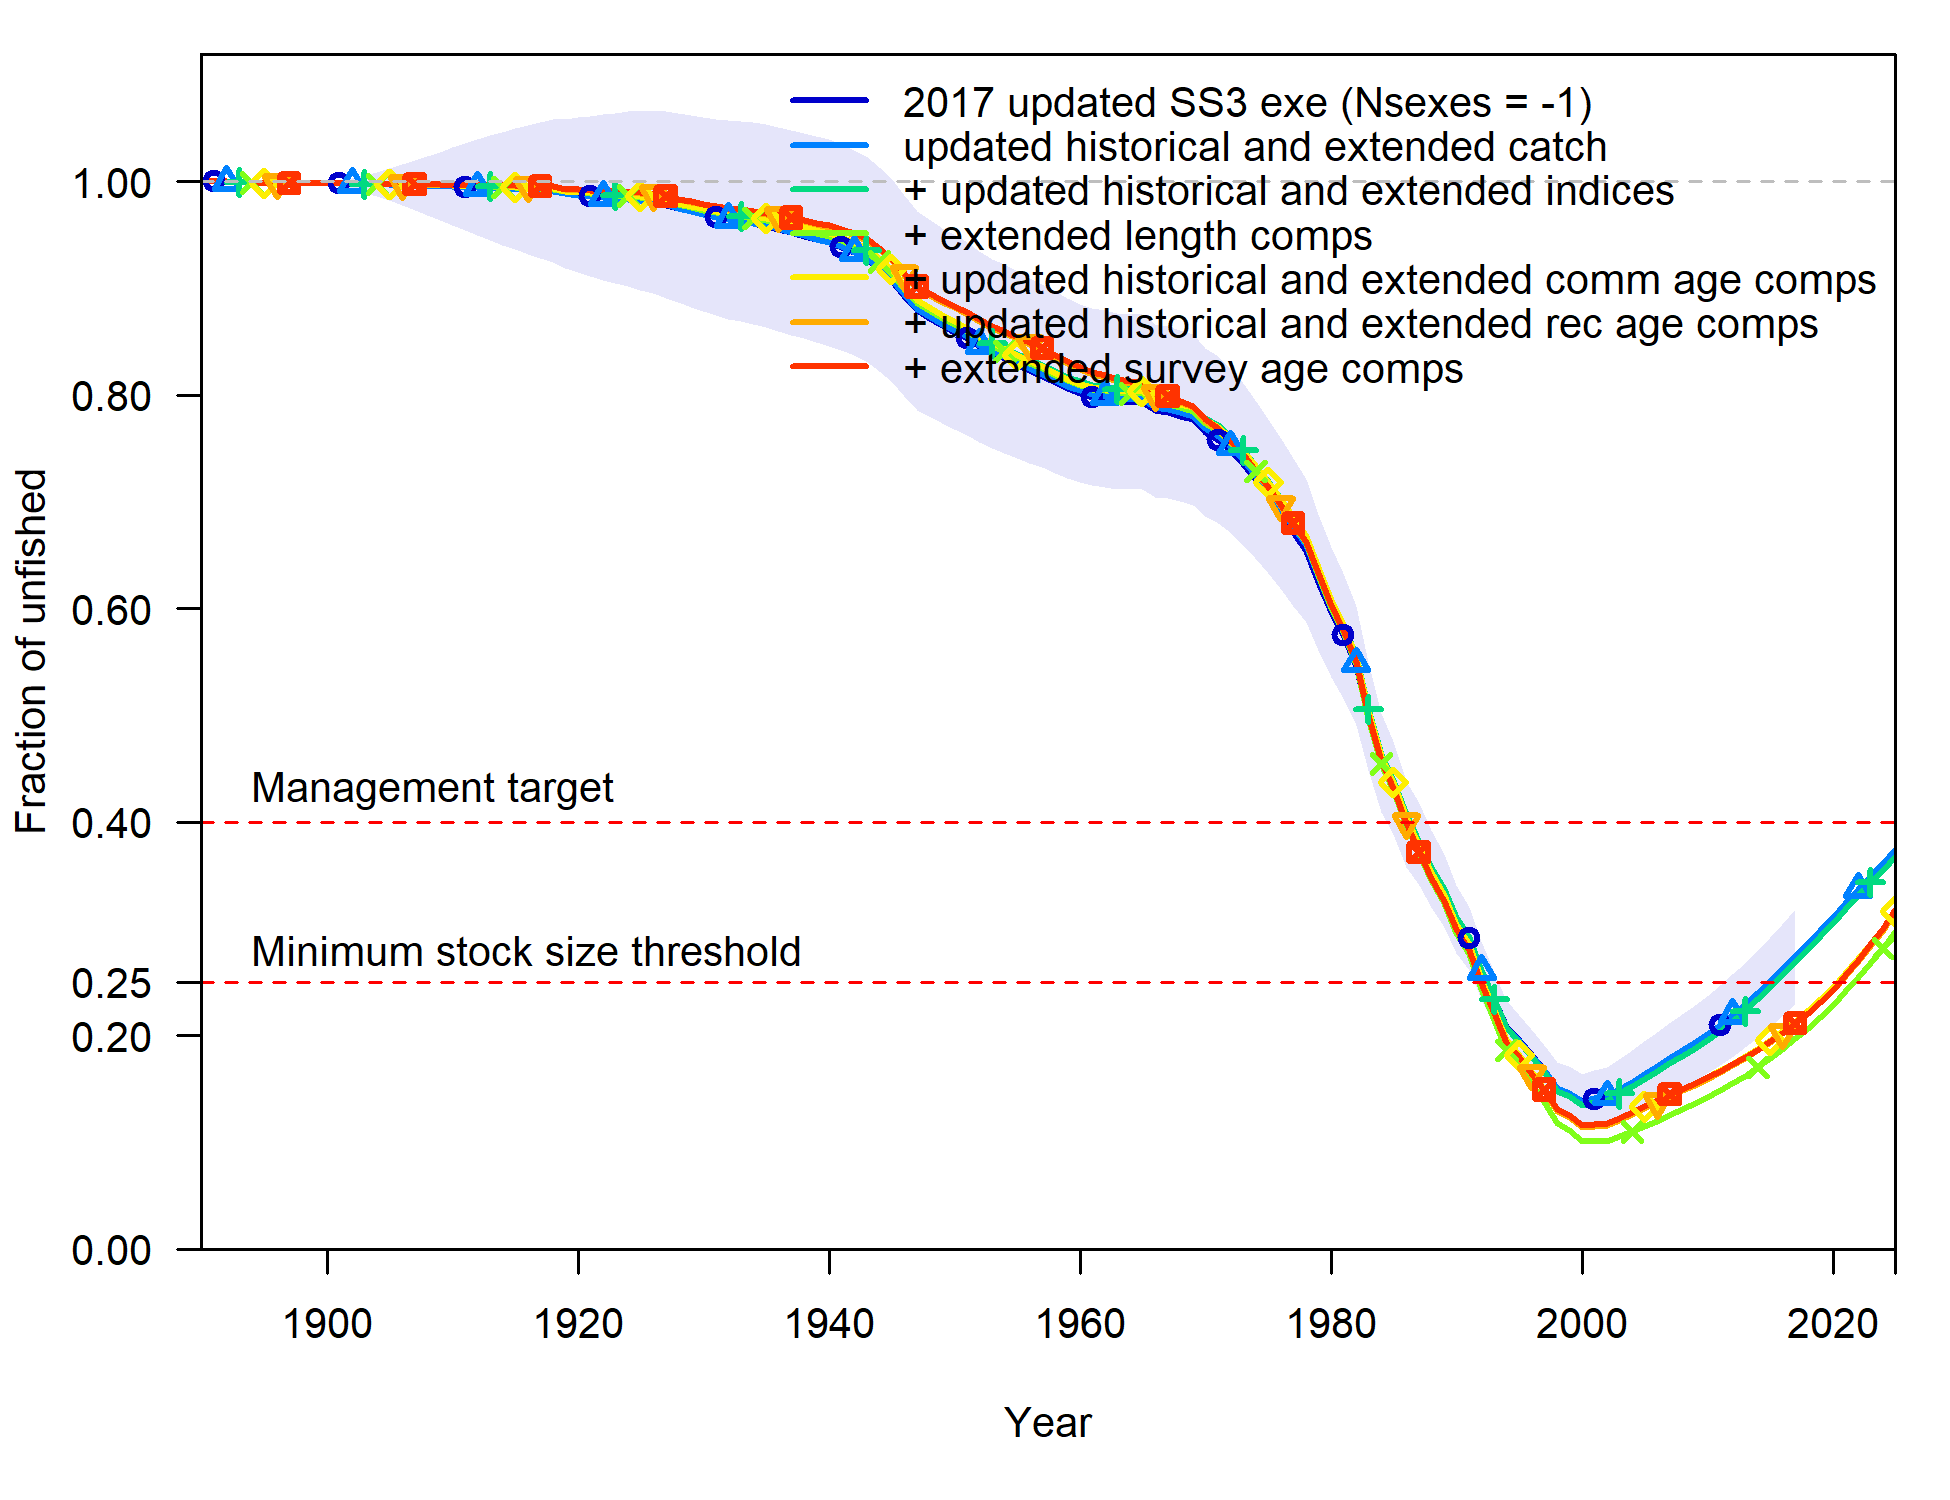
\includegraphics[width=6.5in,height=\textheight,keepaspectratio]{figures/bridging/13_newagecomps/compare4_Bratio_uncertainty.png}

}

\caption{\label{fig-newdata_4}Comparison of the stock status of the 2017
model with an updated SS3 executable (blue), updated catch data (light
blue), updated indices (dark green), new fishery length composition data
(light green), and commercial (yellow), recreational (orange), and
survey (red) age composition data.}

\end{figure}%

\begin{figure}

\centering{

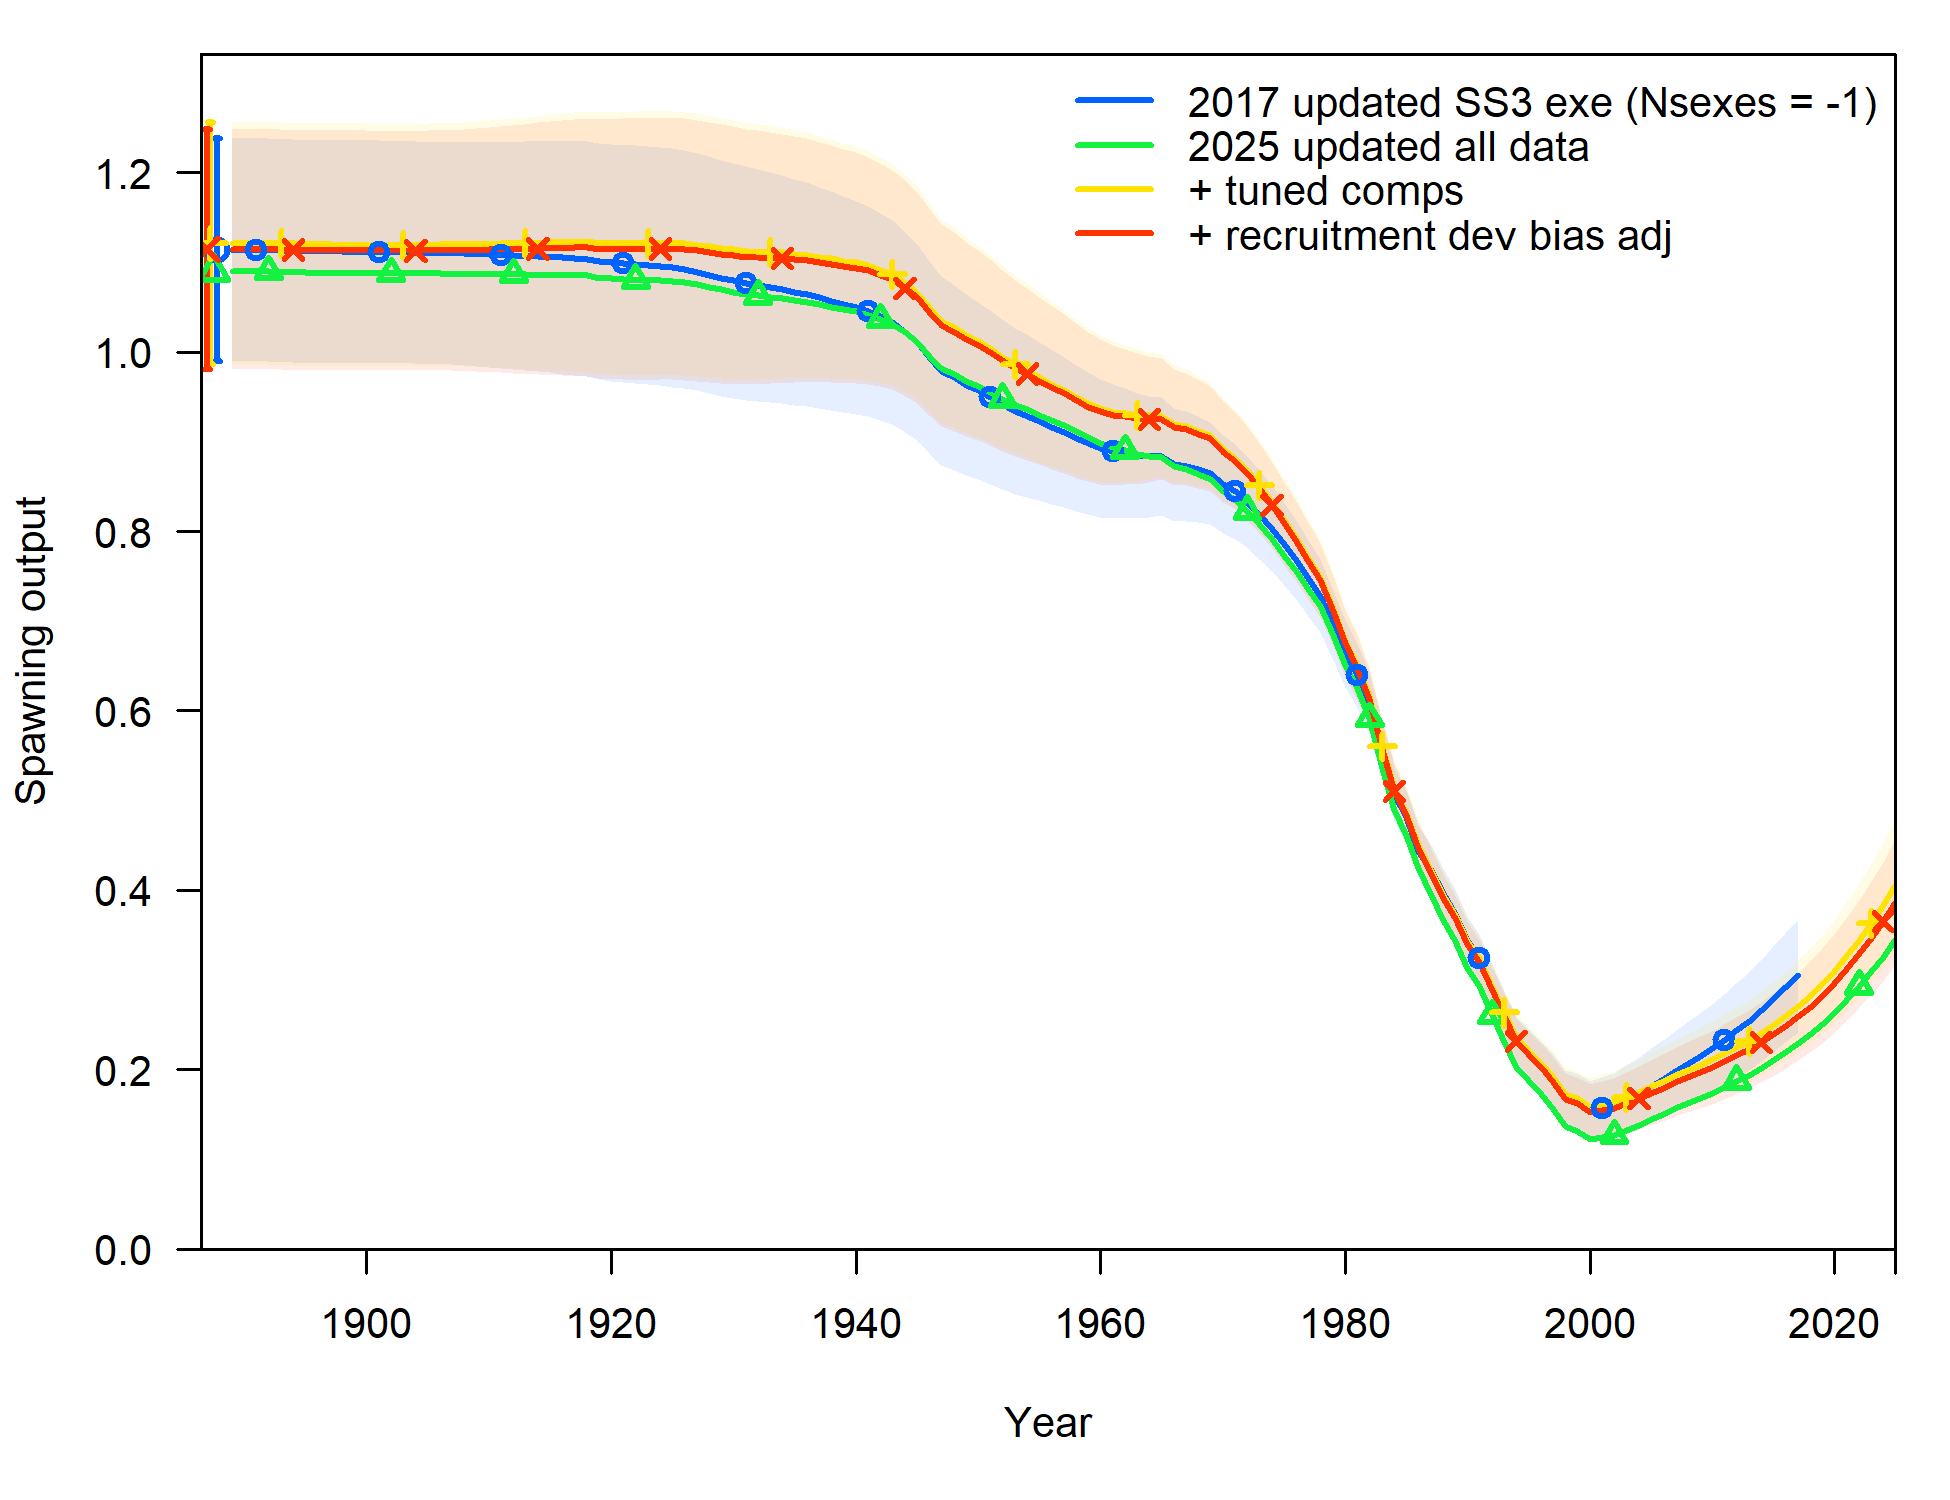
\includegraphics[width=6.5in,height=\textheight,keepaspectratio]{figures/bridging/15_fitbias/compare2_spawnbio_uncertainty.png}

}

\caption{\label{fig-newdata_5}Comparison of the spawning output of the
2017 model with an updated SS3 executable (blue), 2025 model with all
available updated data (green), with tuned compositional data (yellow),
and with the updated recruitment bias adjustment ramp (red).}

\end{figure}%

\begin{figure}

\centering{

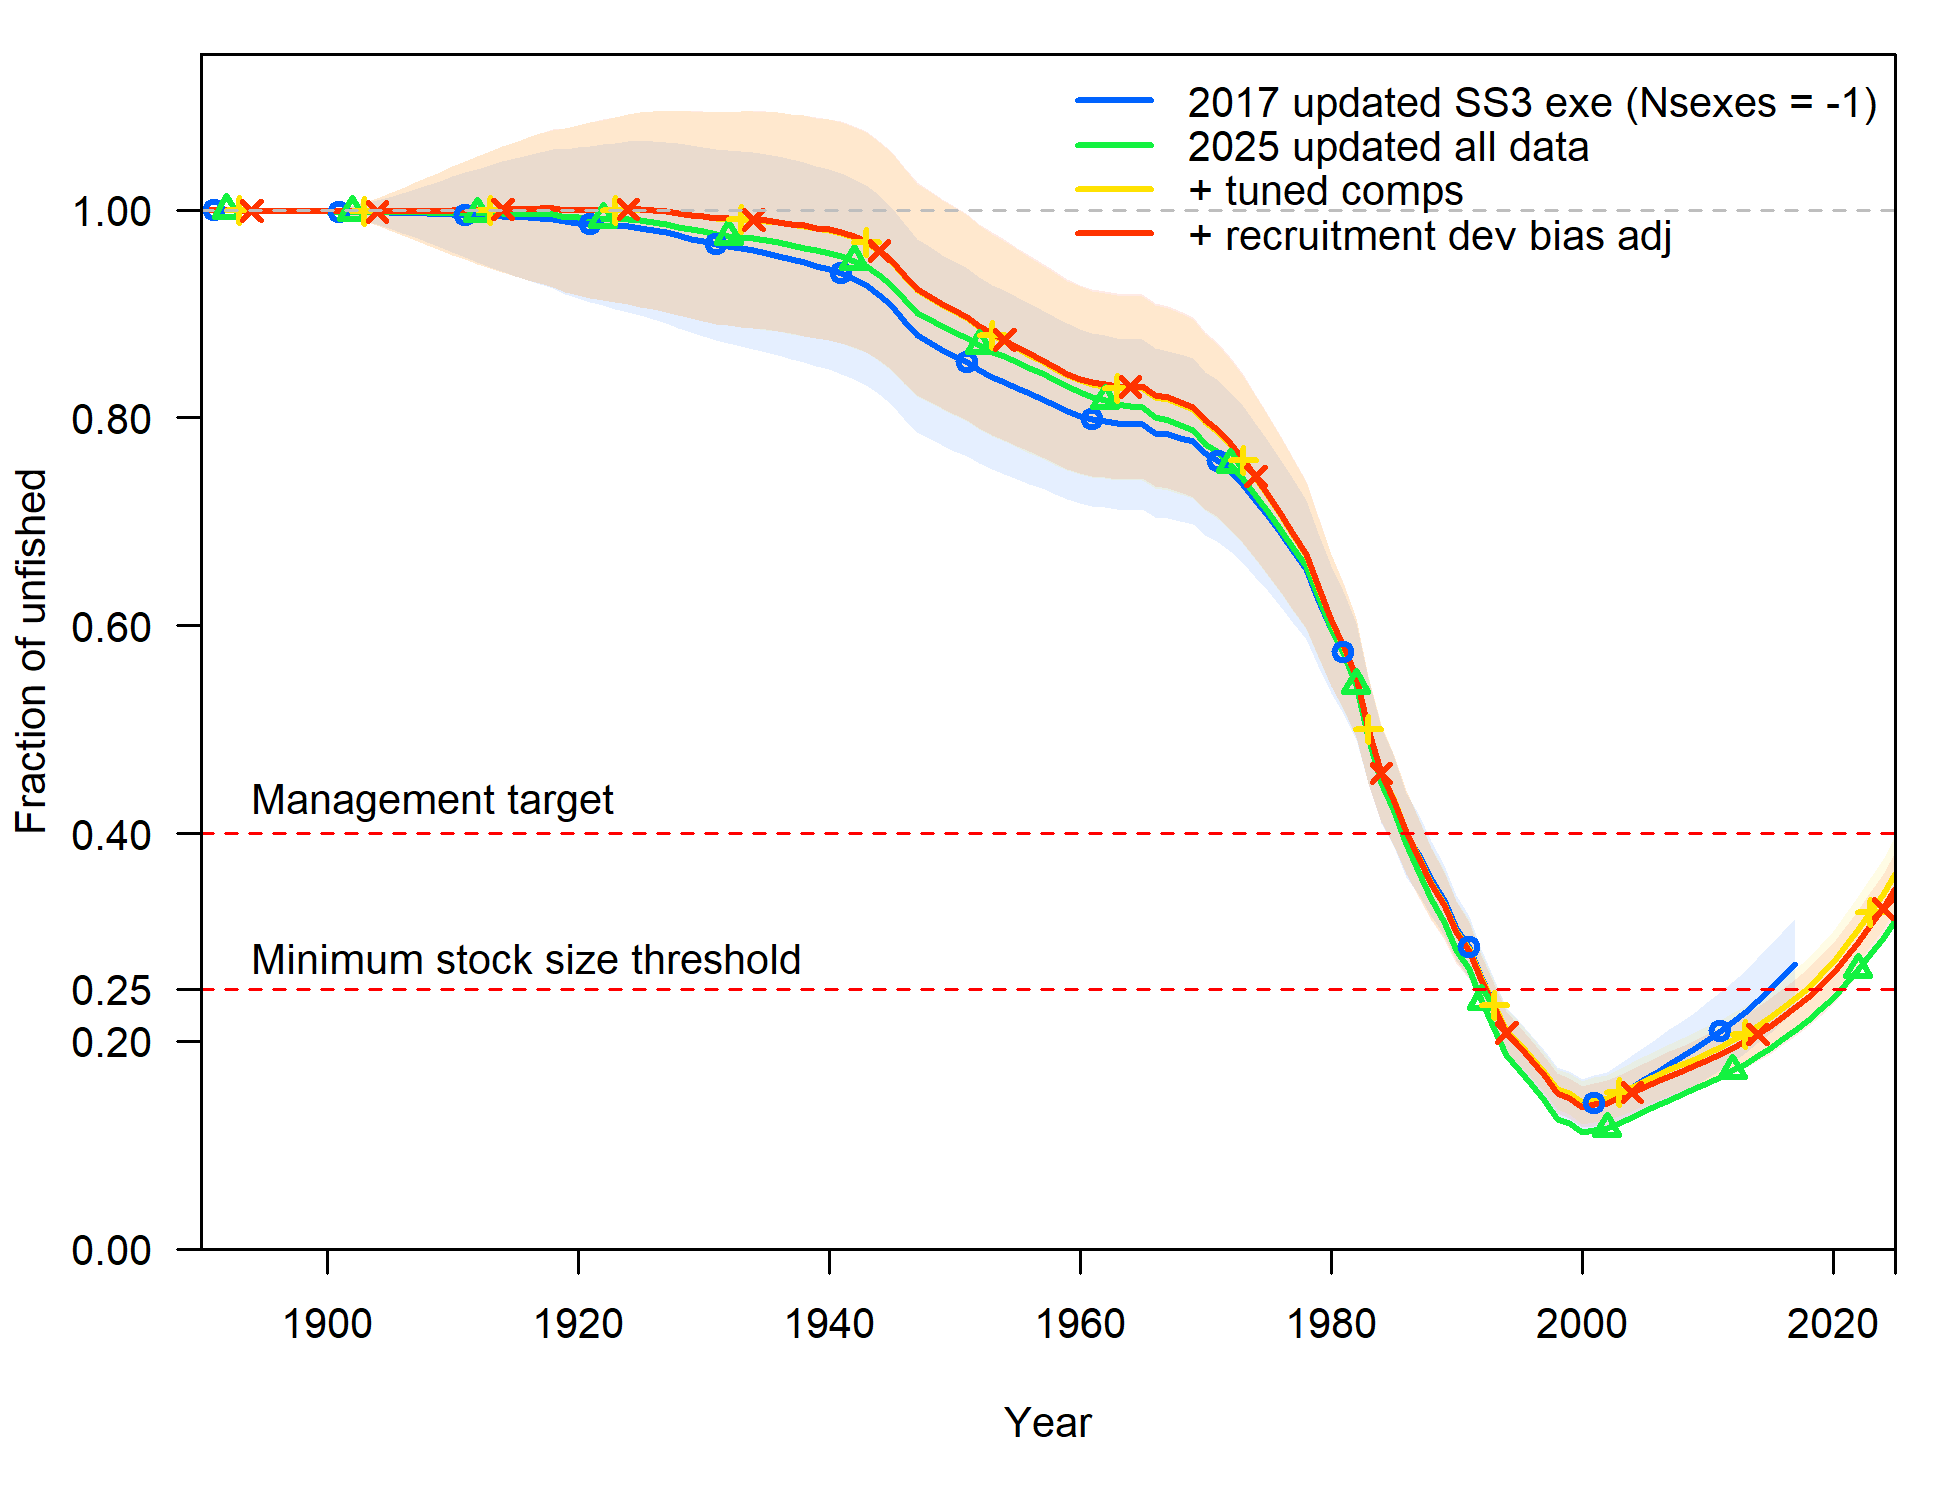
\includegraphics[width=6.5in,height=\textheight,keepaspectratio]{figures/bridging/15_fitbias/compare4_Bratio_uncertainty.png}

}

\caption{\label{fig-newdata_6}Comparison of the stock status of the 2017
model with an updated SS3 executable (blue), 2025 model with all
available updated data (green), with tuned compositional data (yellow),
and with the updated recruitment bias adjustment ramp (red).}

\end{figure}%

\begin{figure}

\centering{

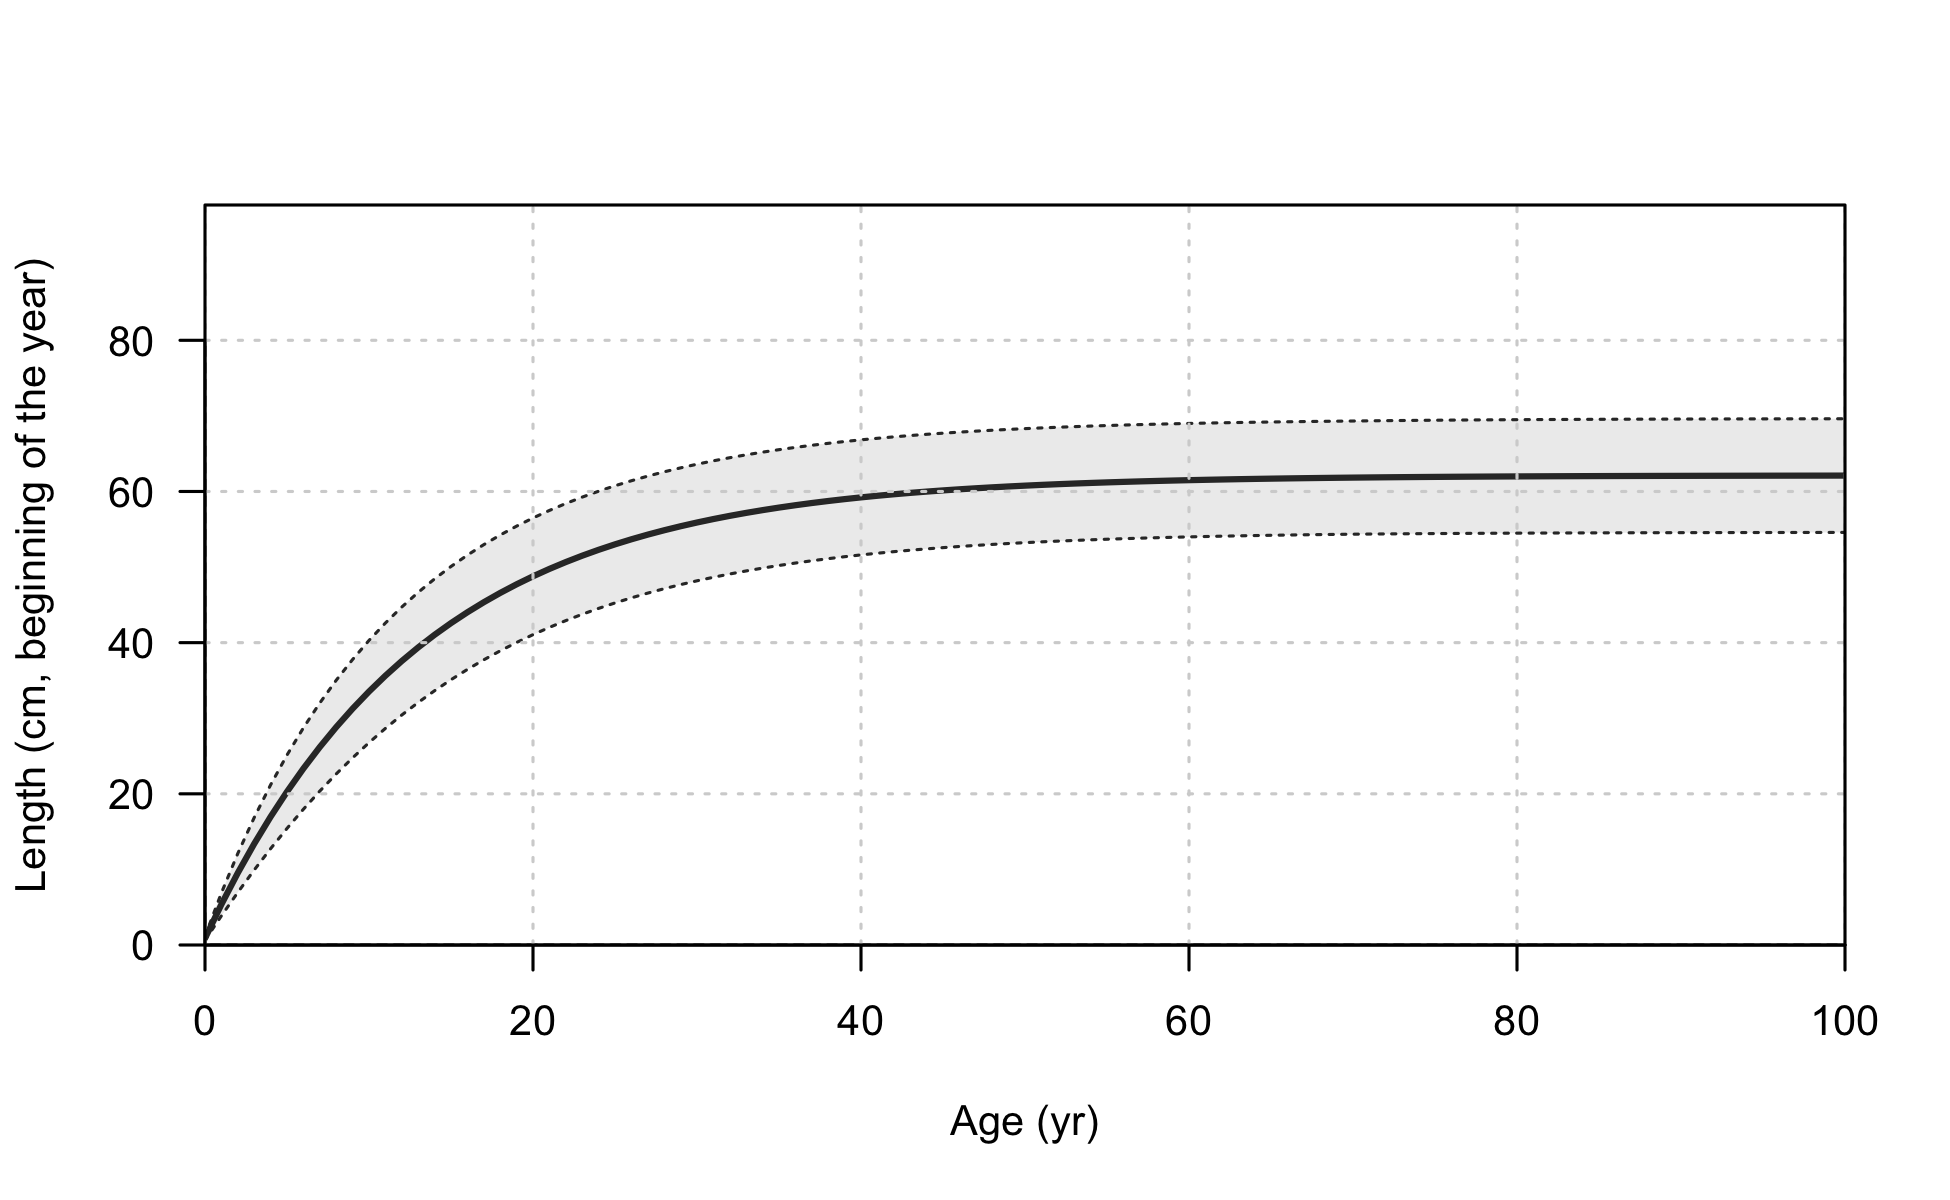
\includegraphics[width=6.5in,height=\textheight,keepaspectratio]{figures/r4ss_plots/plots/bio1_sizeatage.png}

}

\caption{\label{fig-growth}Length at age in the beginning of the year in
the ending year of the model.}

\end{figure}%

\begin{figure}

\centering{

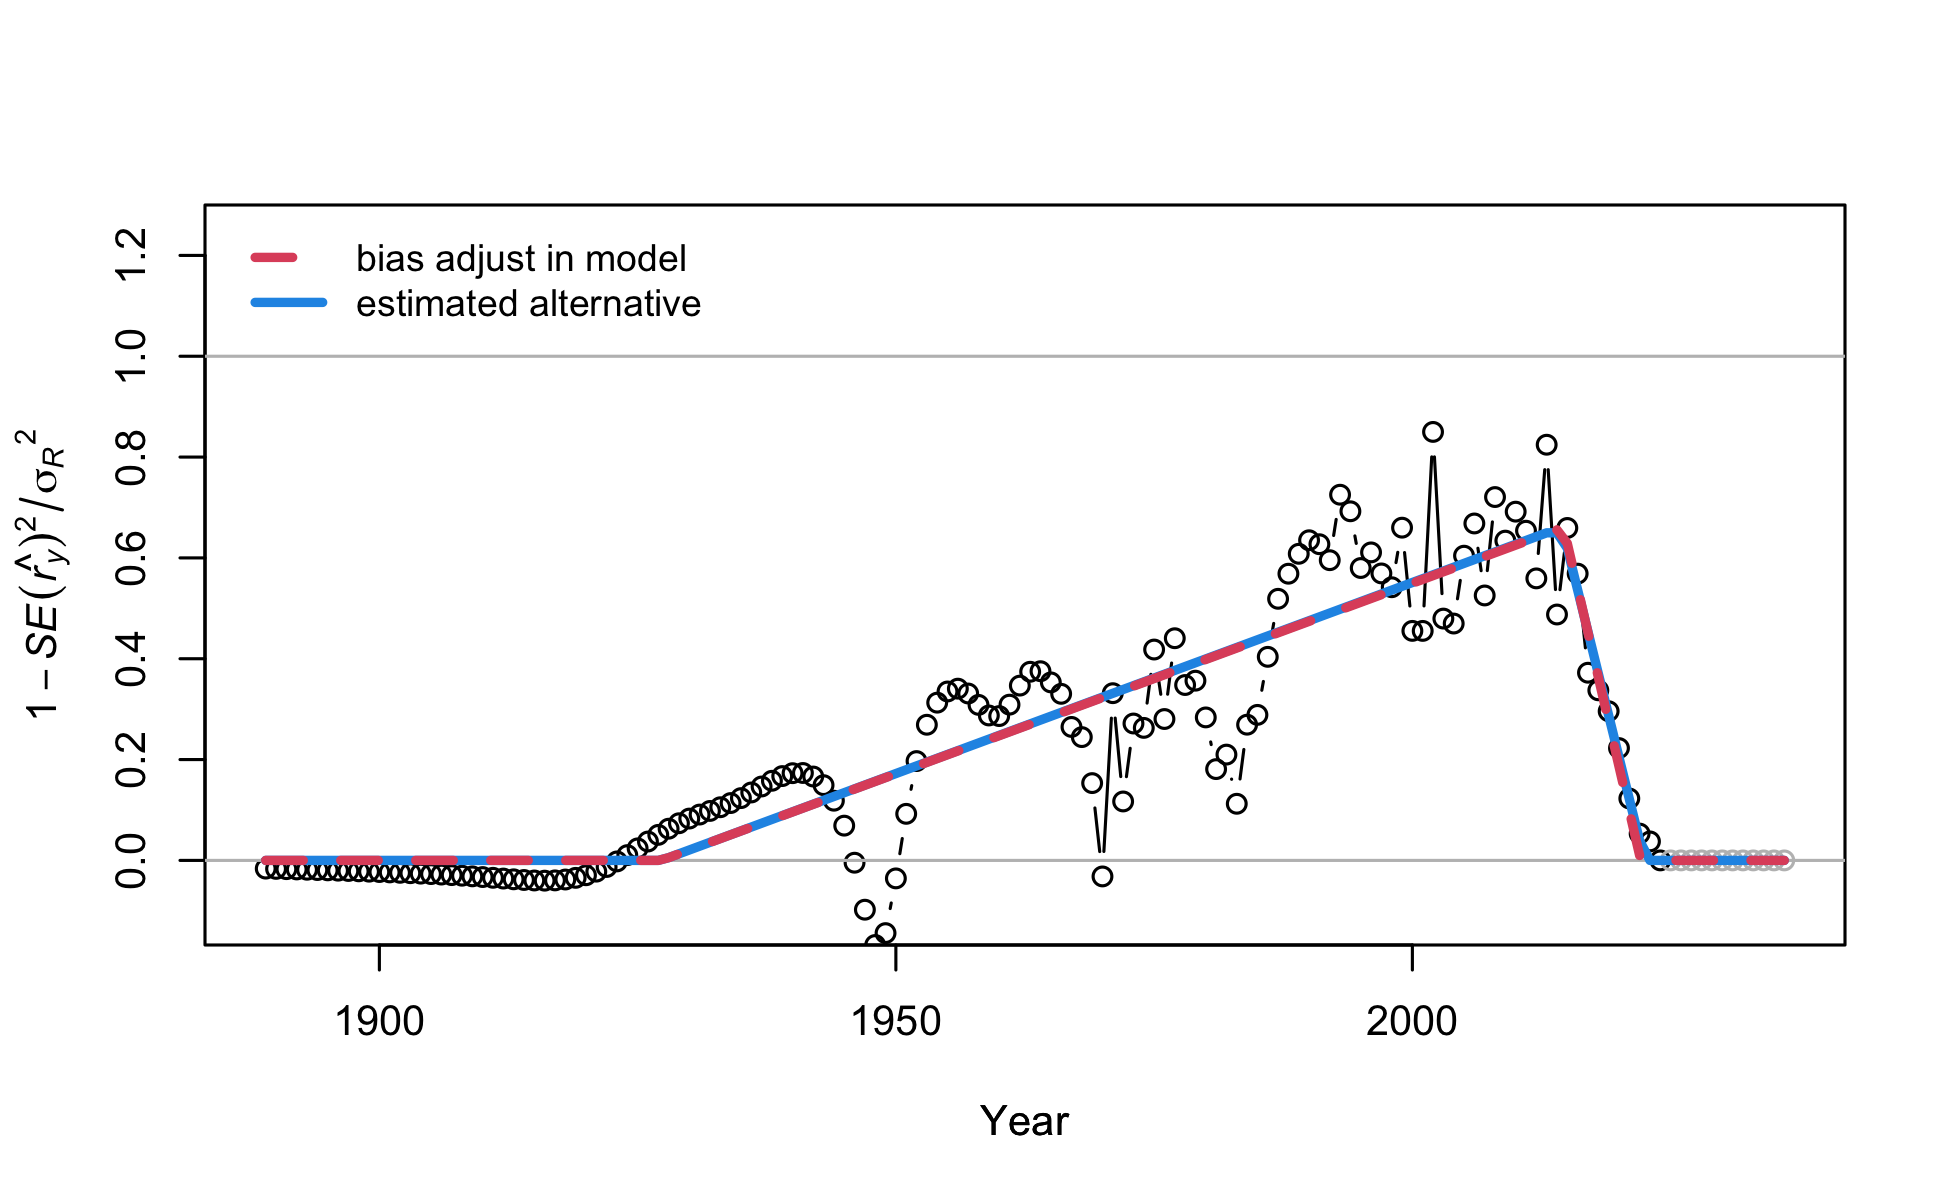
\includegraphics[width=6.5in,height=\textheight,keepaspectratio]{figures/r4ss_plots/plots/recruit_fit_bias_adjust.png}

}

\caption{\label{fig-biasadj}Points are transformed variances. Red line
shows current settings for bias adjustment specified in the control
file. Blue line shows least squares estimate of alternative bias
adjustment relationship for recruitment deviations.}

\end{figure}%

\clearpage

\begin{figure}

\centering{

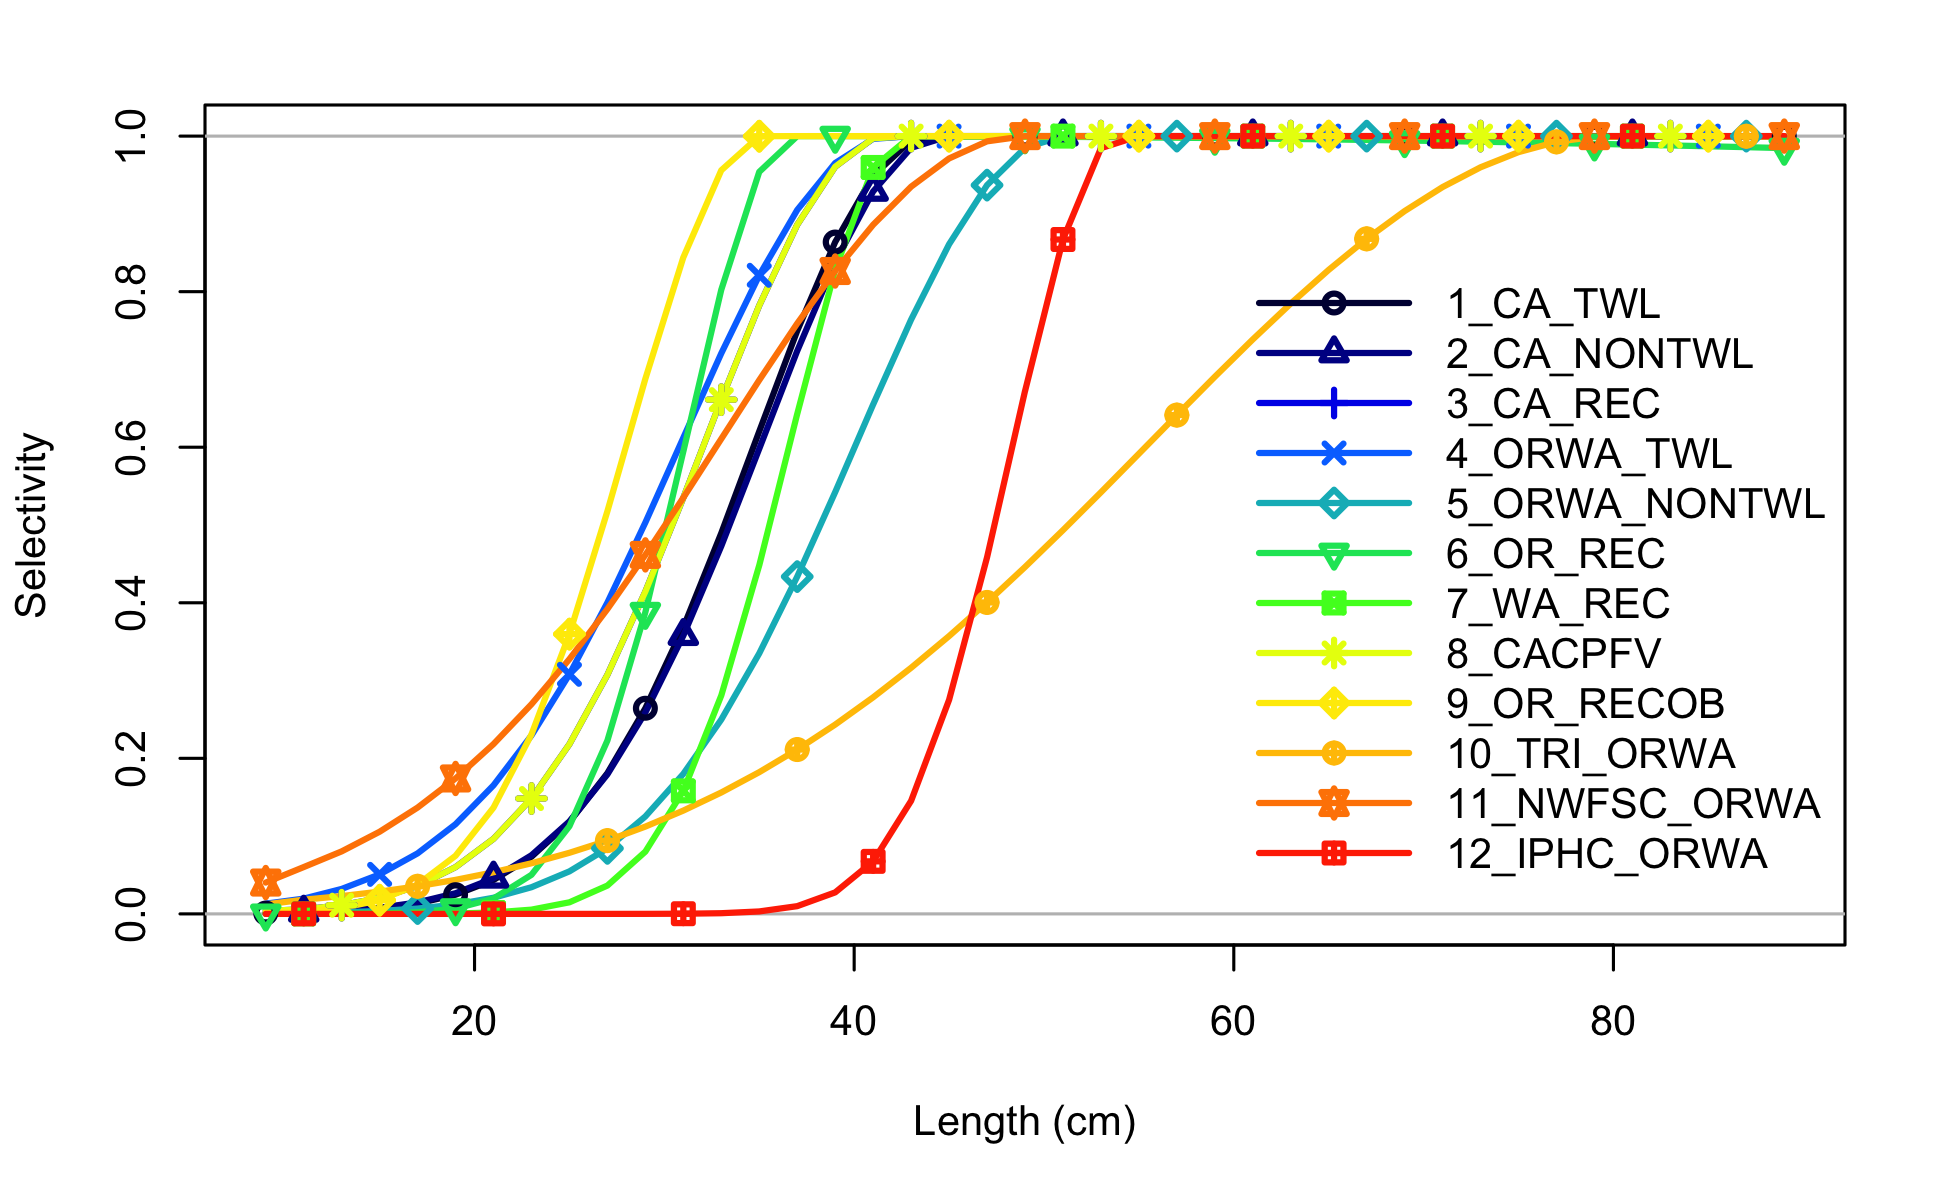
\includegraphics[width=6.5in,height=\textheight,keepaspectratio]{figures/r4ss_plots/plots/sel01_multiple_fleets_length1.png}

}

\caption{\label{fig-selex_allfleets}Estimated selectivity at length for
all fleets.}

\end{figure}%

\begin{figure}

\centering{

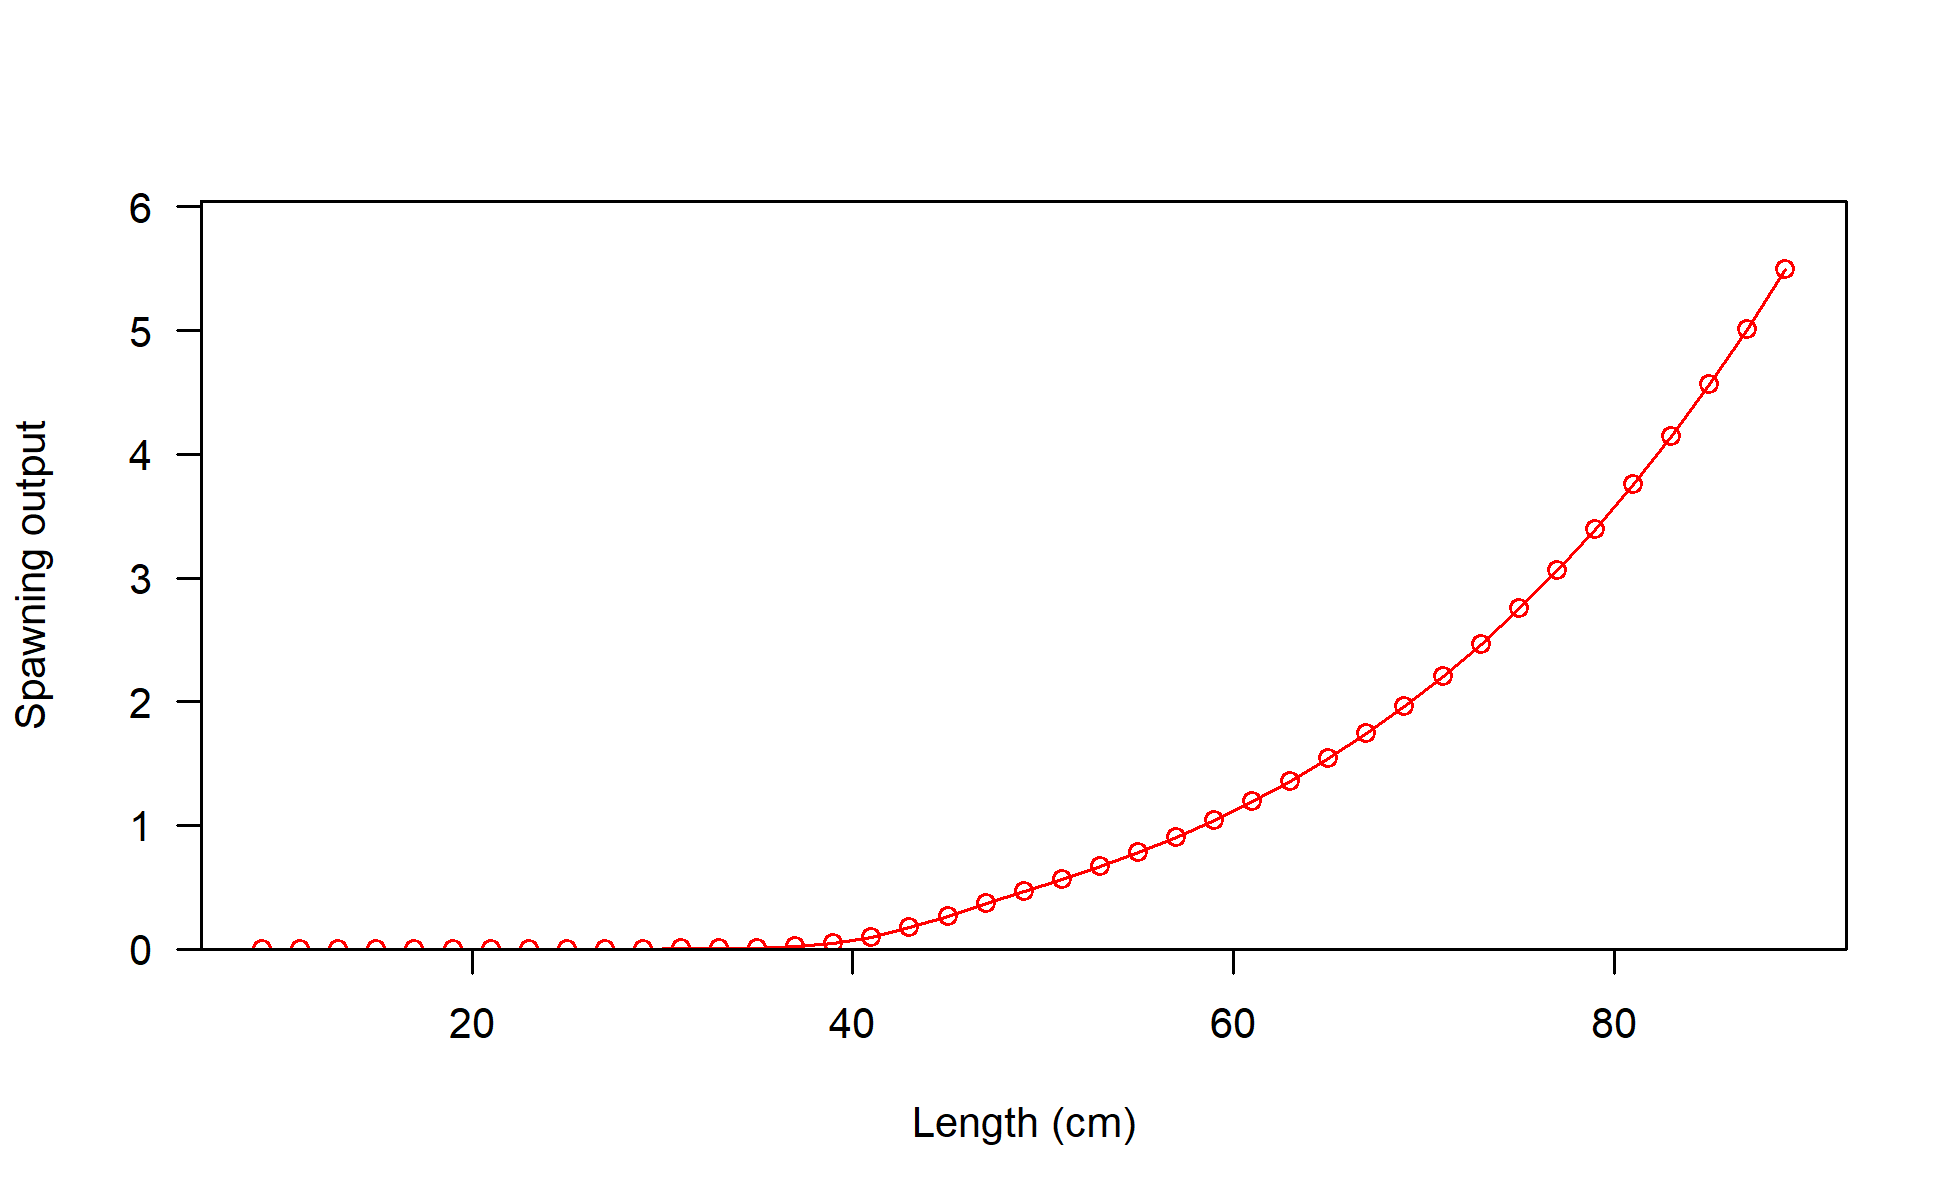
\includegraphics[width=6.5in,height=\textheight,keepaspectratio]{figures/r4ss_plots/plots/bio10_spawningoutput_len.png}

}

\caption{\label{fig-spoutlen}Spawning output at length.}

\end{figure}%

\begin{figure}

\centering{

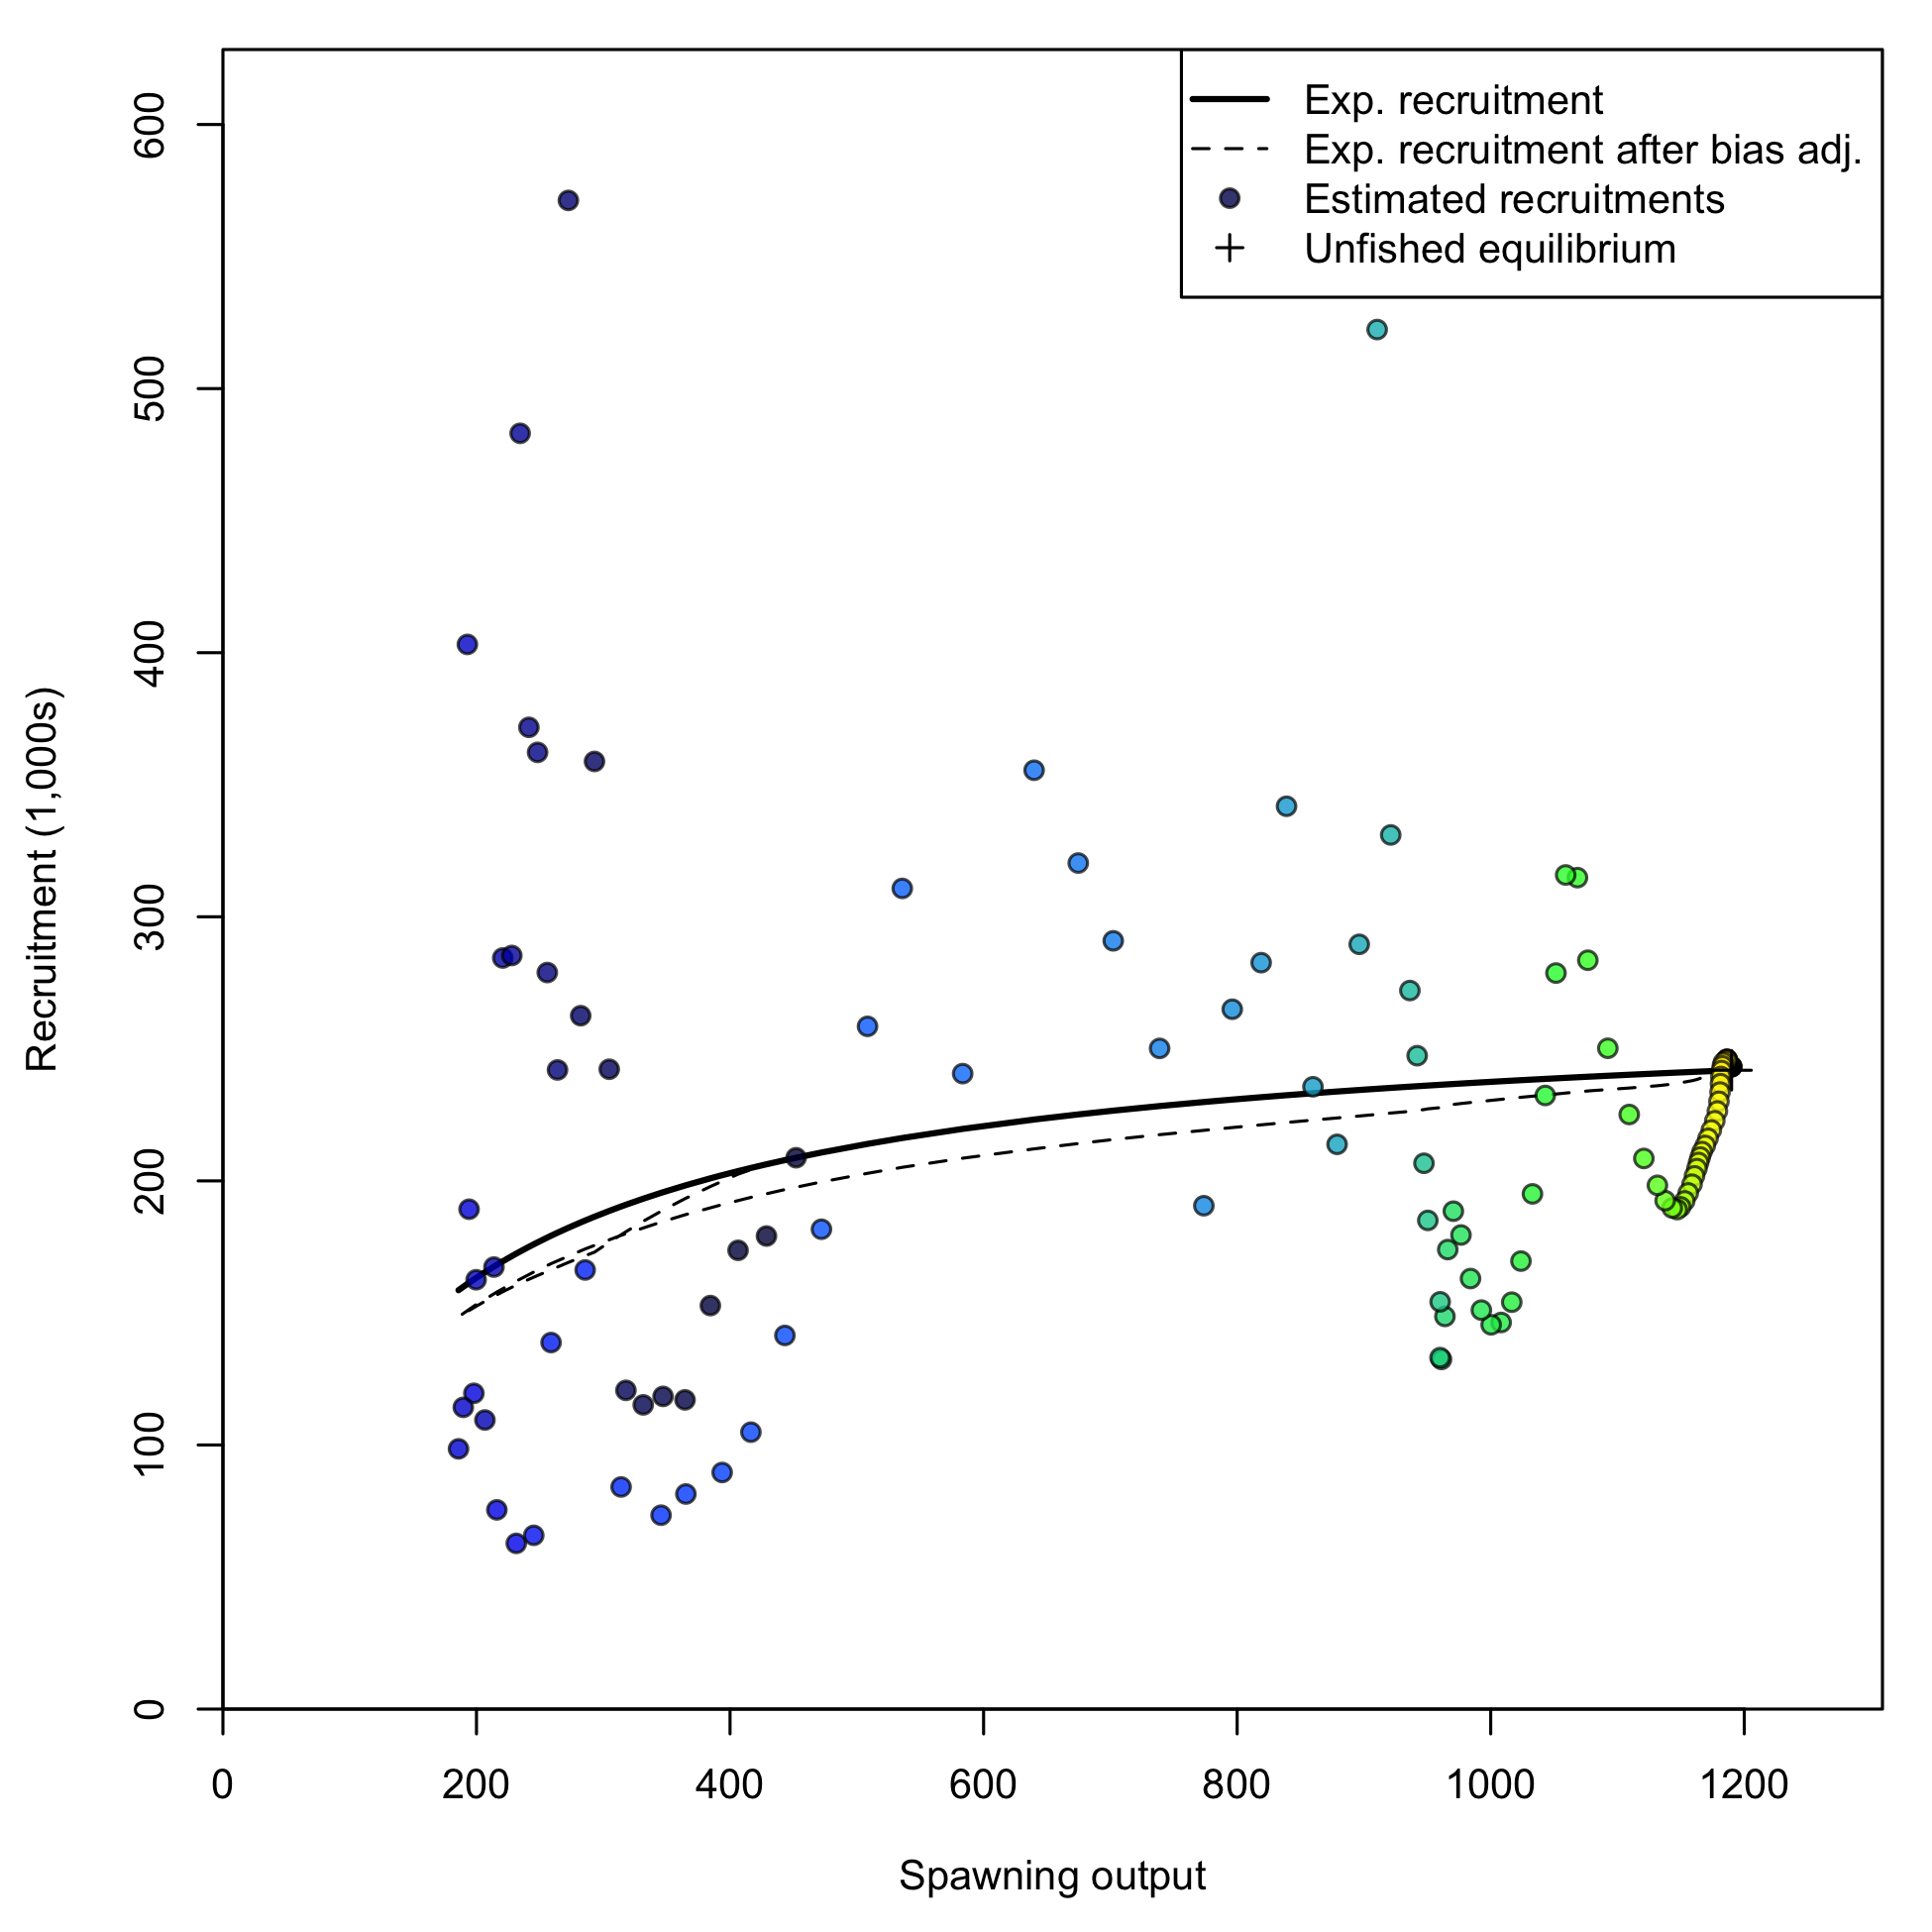
\includegraphics[width=6.5in,height=\textheight,keepaspectratio]{figures/r4ss_plots/plots/SR_curve.png}

}

\caption{\label{fig-SRcurve}Stock-recruit curve. Point colors indicate
year, with warmer colors indicating earlier years and cooler colors in
showing later years.}

\end{figure}%

\begin{figure}

\centering{

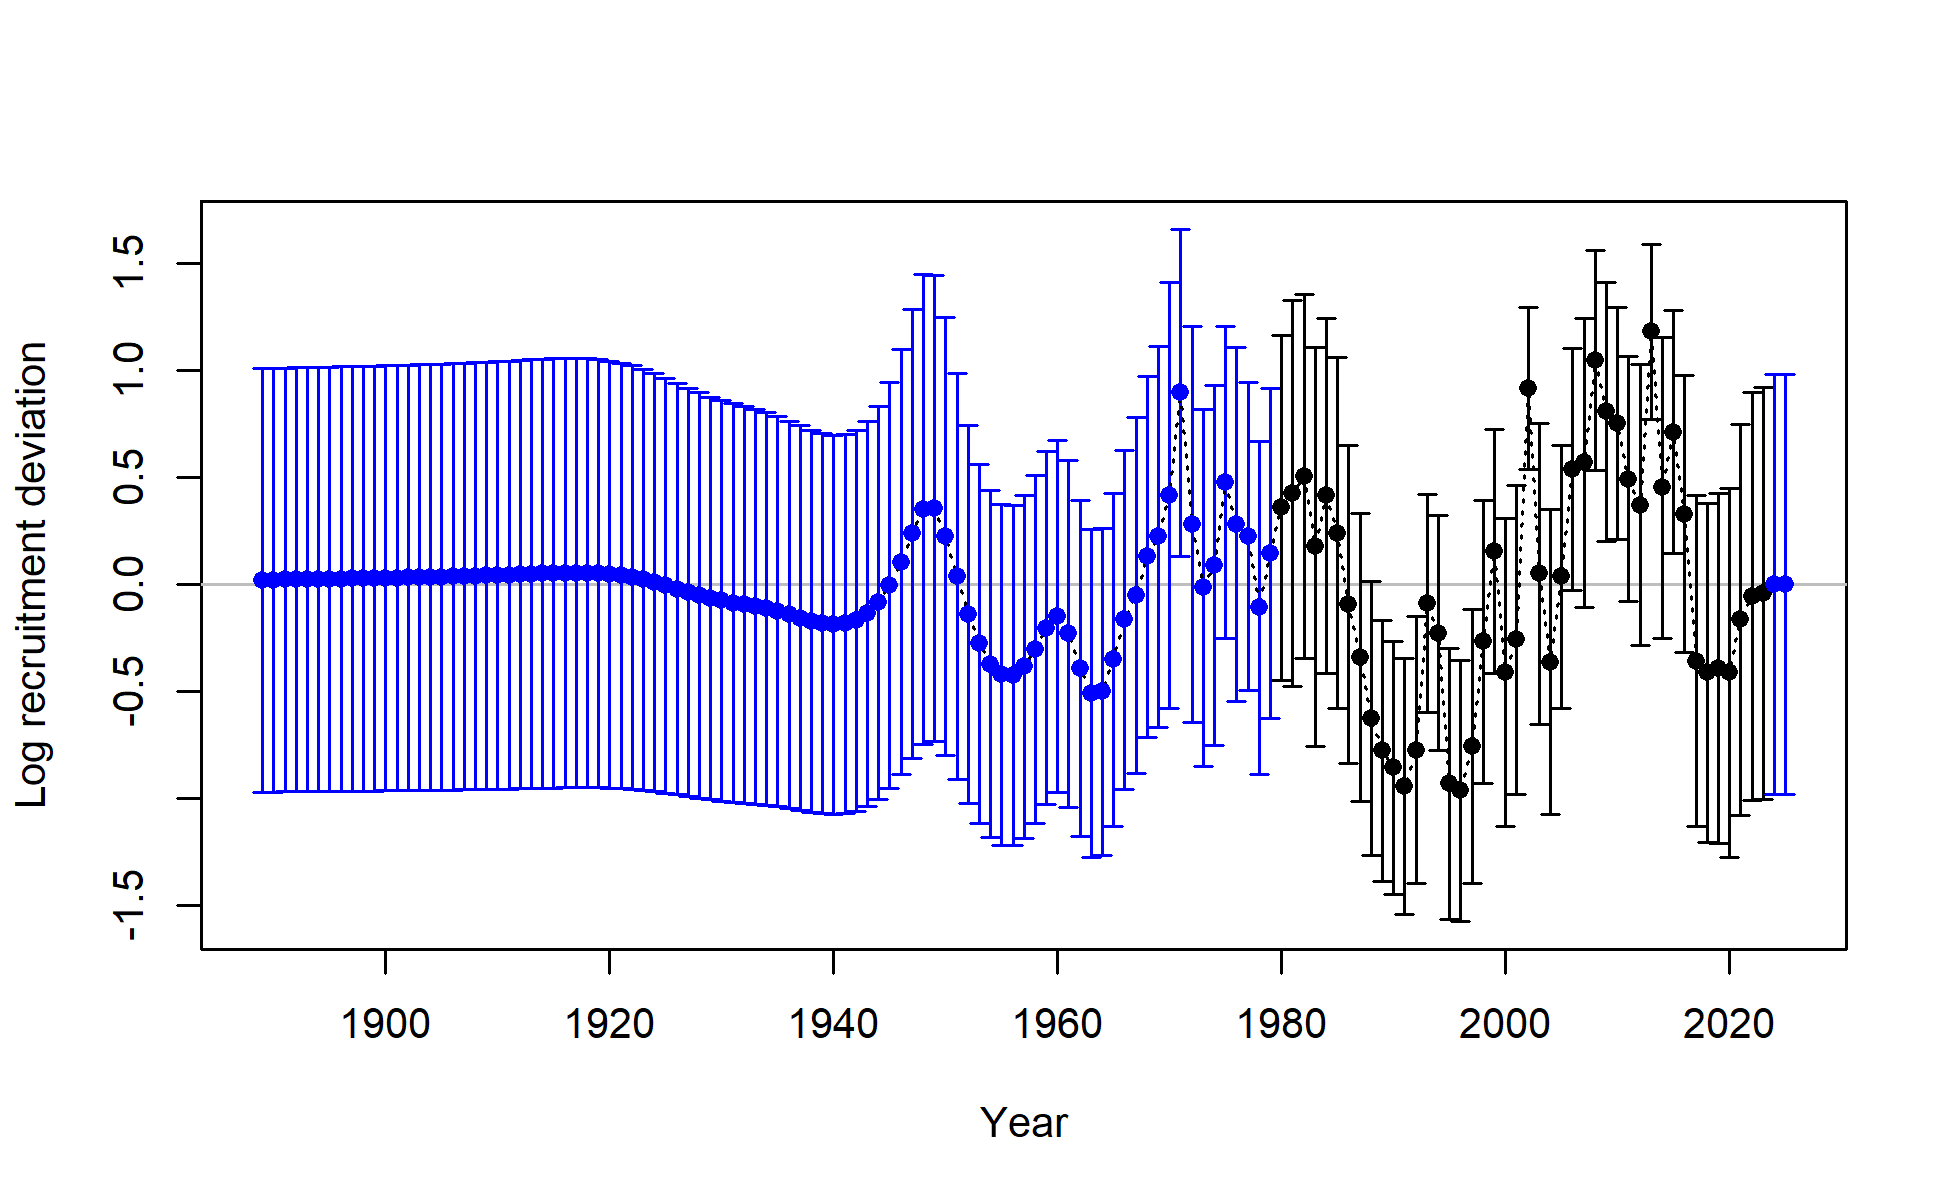
\includegraphics[width=6.5in,height=\textheight,keepaspectratio]{figures/r4ss_plots/plots/recdevs2_withbars.png}

}

\caption{\label{fig-recdevs_err}Estimated recruitment deviations with
95\% intervals.}

\end{figure}%

\begin{figure}

\centering{

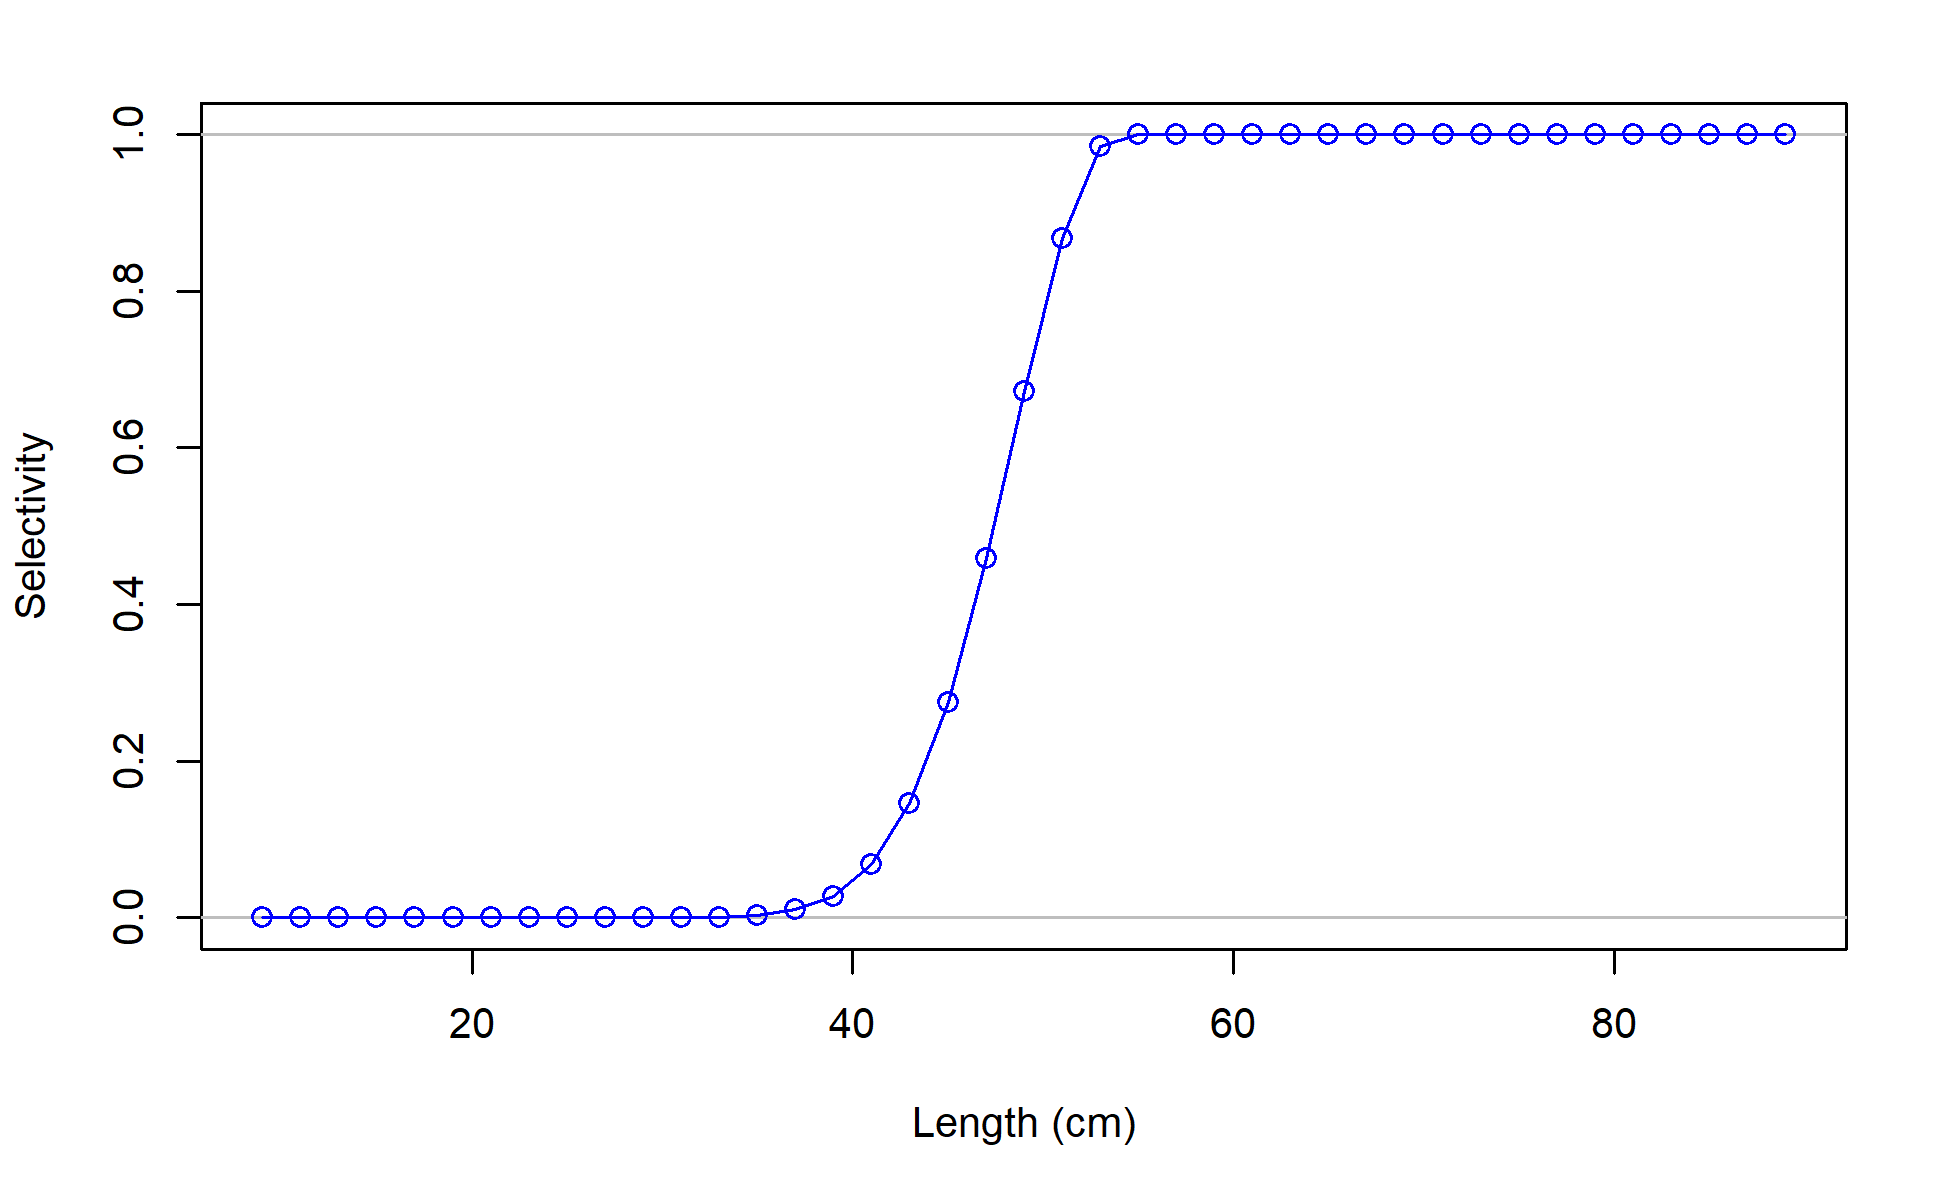
\includegraphics[width=6.5in,height=\textheight,keepaspectratio]{figures/r4ss_plots/plots/sel09_len_flt12sex1.png}

}

\caption{\label{fig-sel12}Estimated selectivity for the IPHC longline
survey for Oregon/Washington (Fleet 12).}

\end{figure}%

\begin{figure}

\centering{

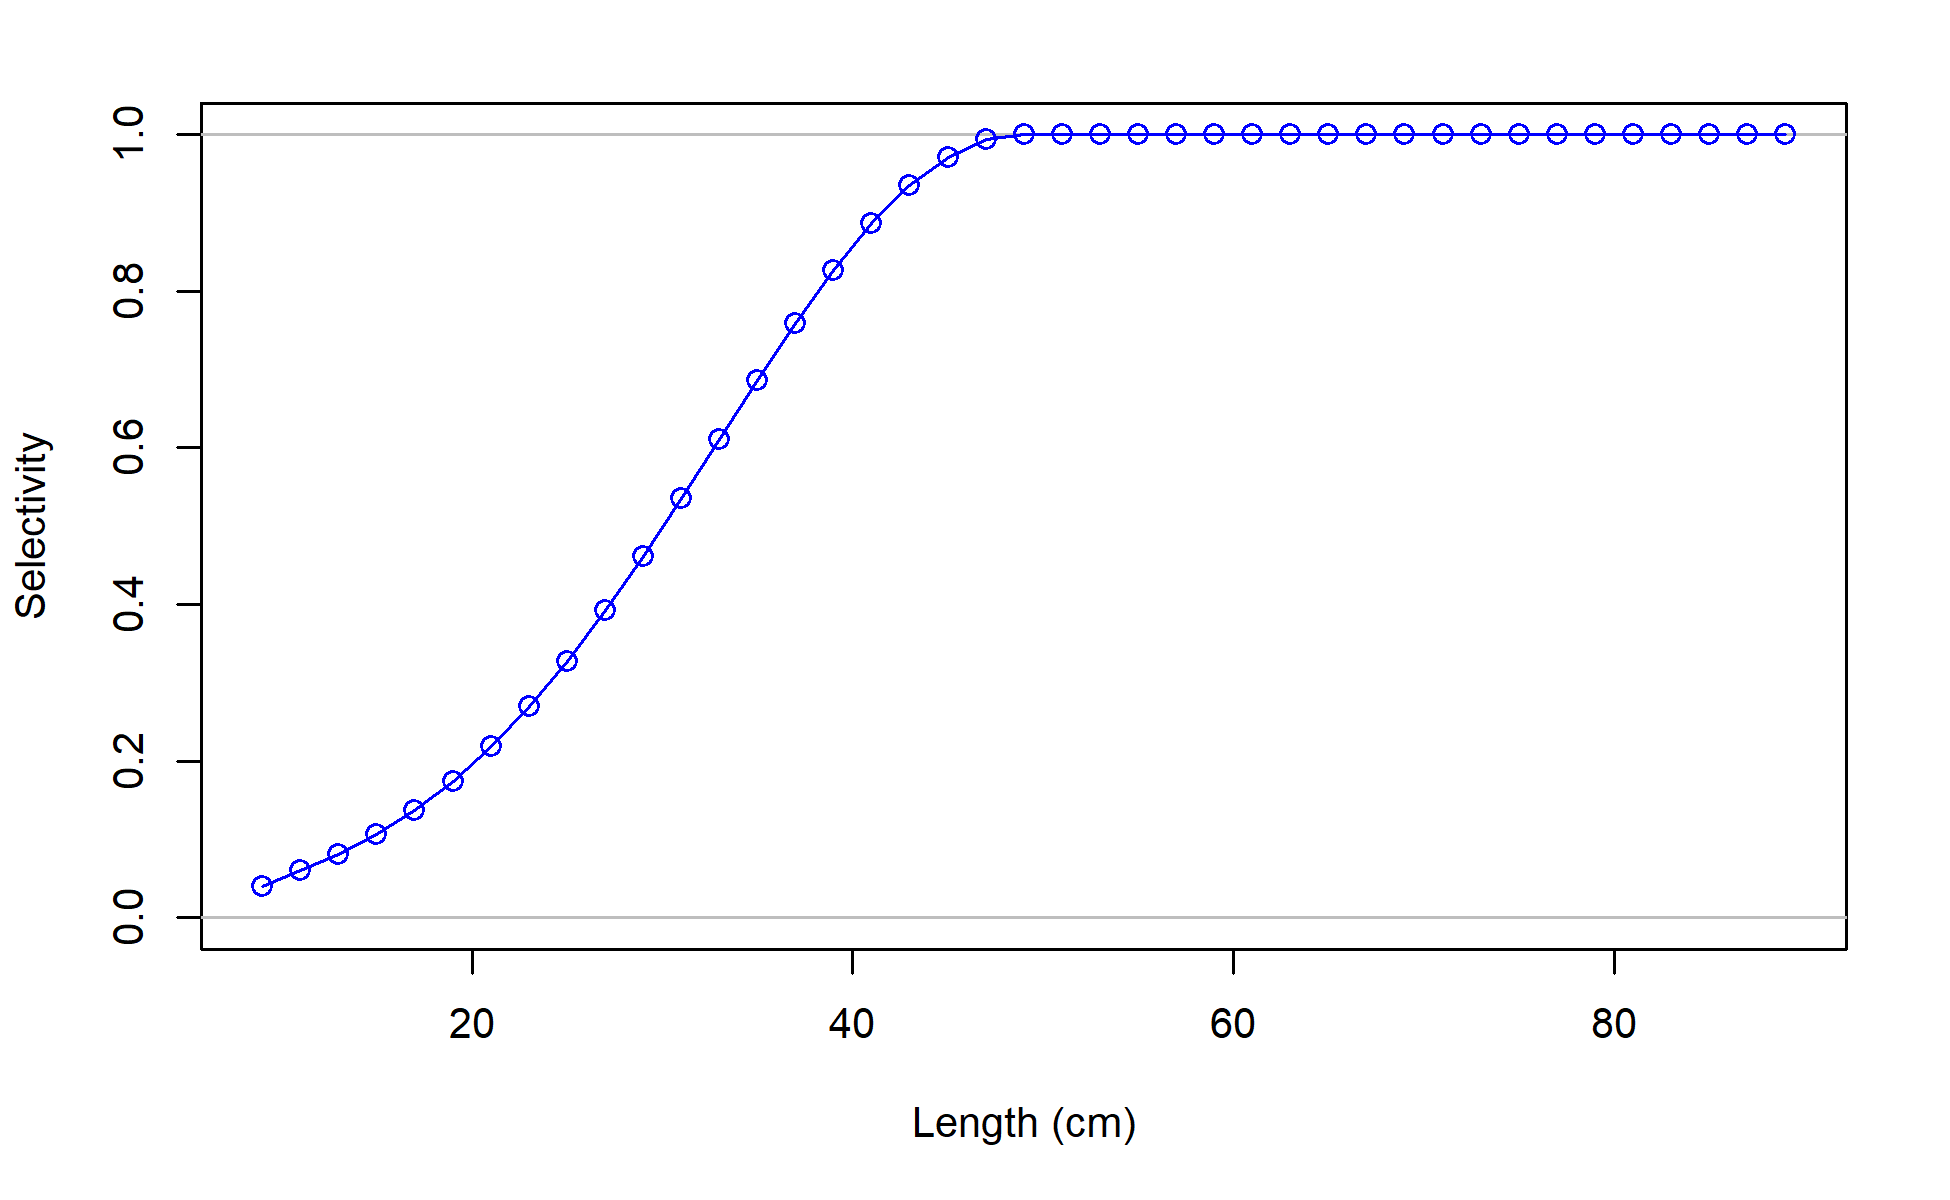
\includegraphics[width=6.5in,height=\textheight,keepaspectratio]{figures/r4ss_plots/plots/sel09_len_flt11sex1.png}

}

\caption{\label{fig-sel11}Estimated selectivity for the WCBTS for
Oregon/Washington (Fleet 11).}

\end{figure}%

\begin{figure}

\centering{

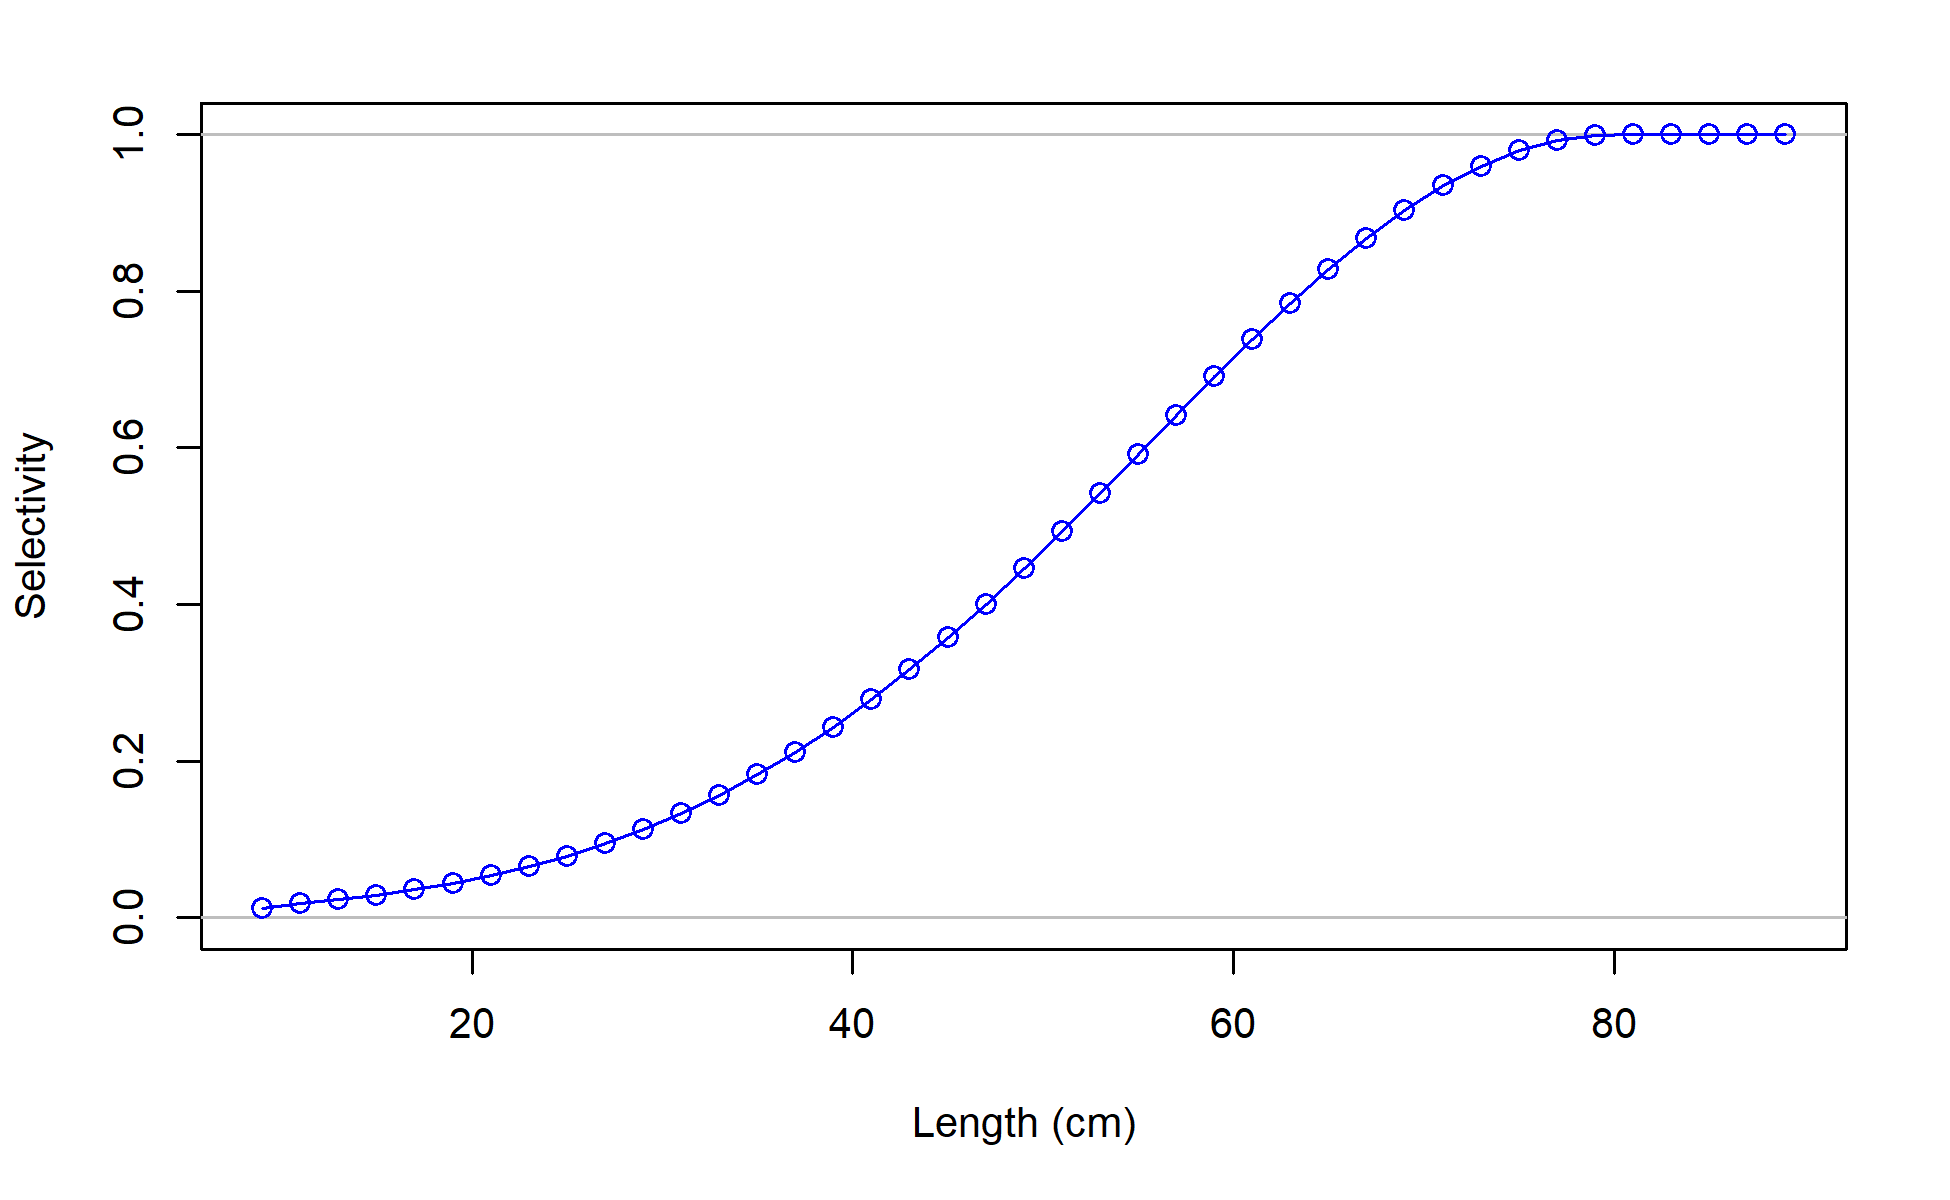
\includegraphics[width=6.5in,height=\textheight,keepaspectratio]{figures/r4ss_plots/plots/sel09_len_flt10sex1.png}

}

\caption{\label{fig-sel10}Estimated selectivity for the Triennial bottom
trawl survey for Oregon/Washington (Fleet 10).}

\end{figure}%

\clearpage

\begin{figure}

\centering{

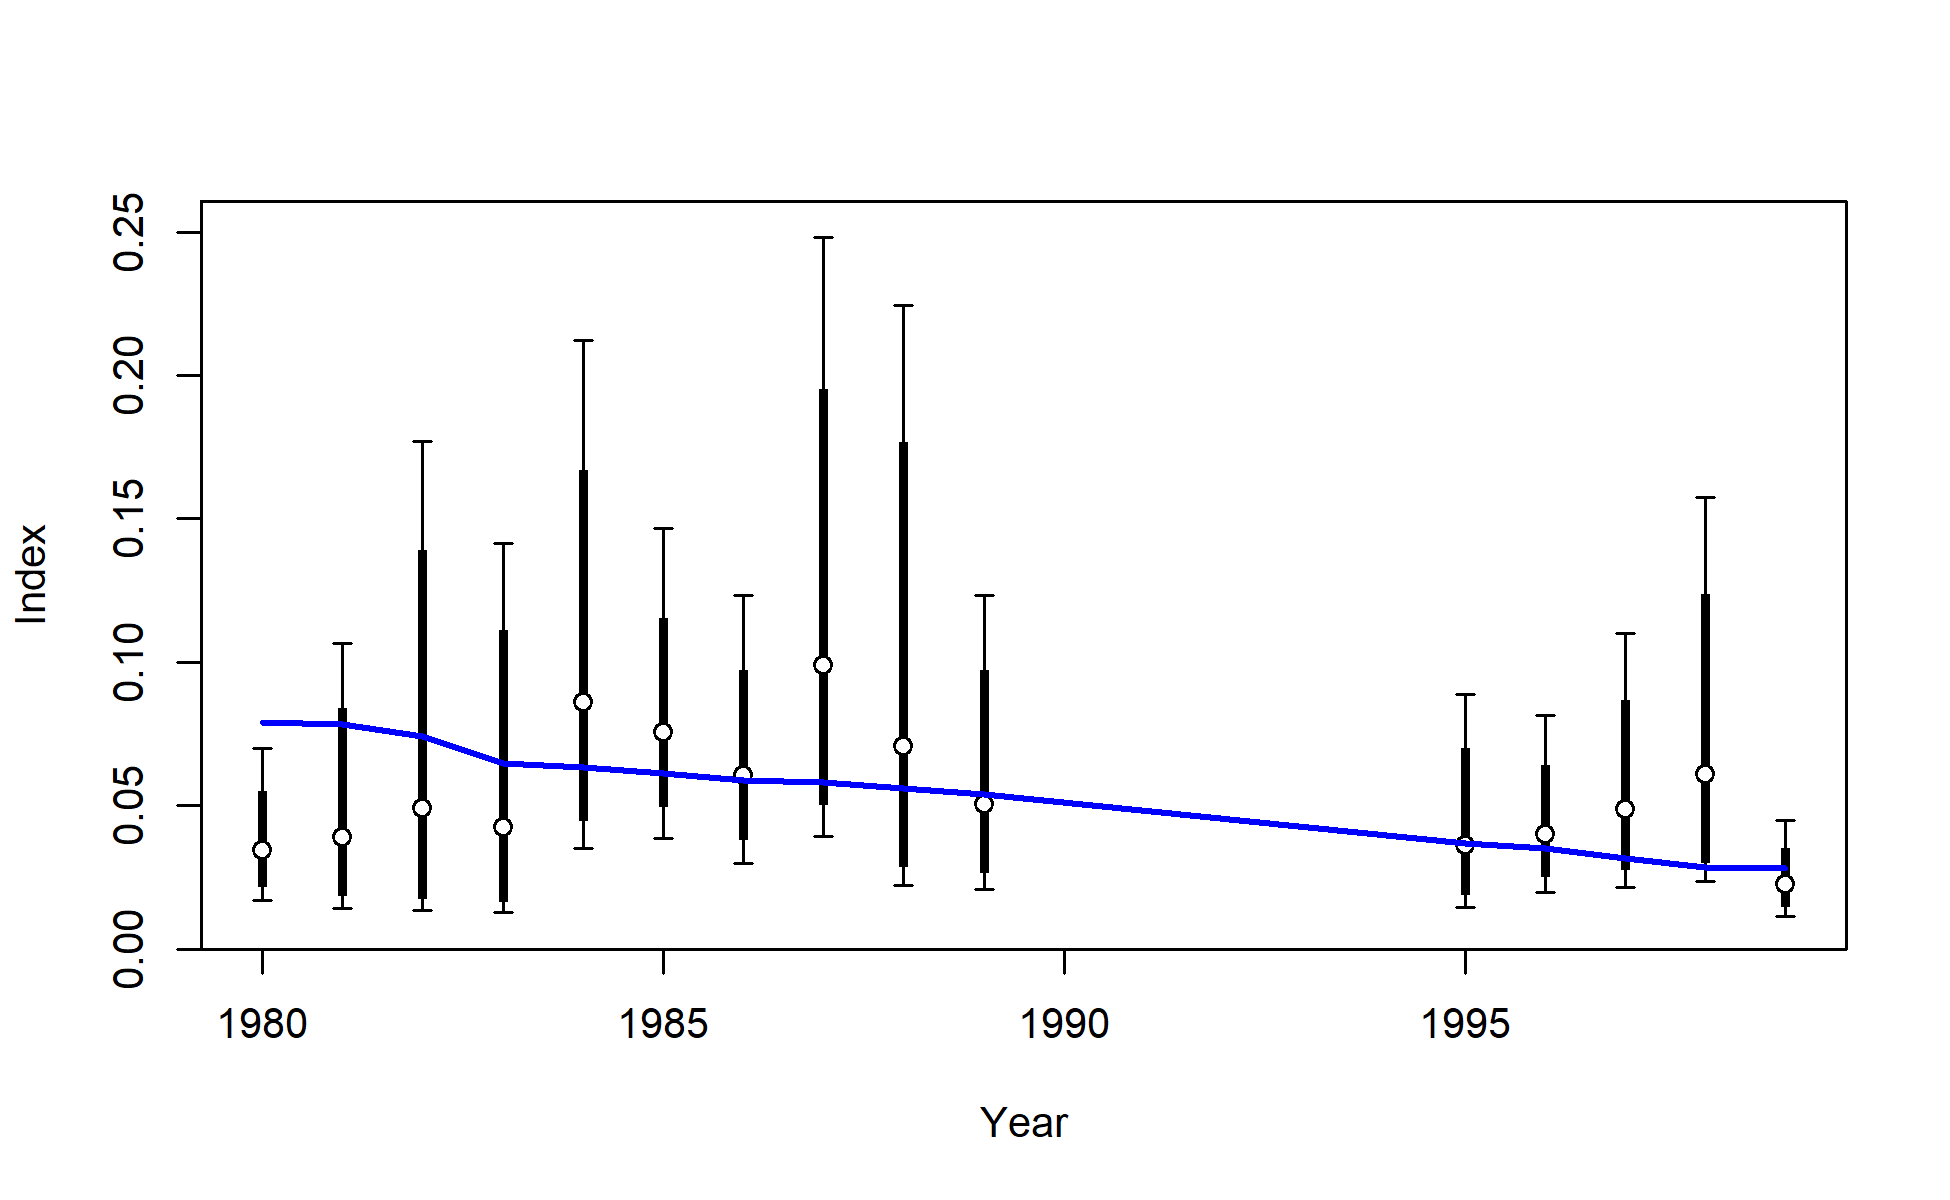
\includegraphics[width=6.5in,height=\textheight,keepaspectratio]{figures/r4ss_plots/plots/index2_cpuefit_3_CA_REC.png}

}

\caption{\label{fig-indexfit3}Fit to the California MRFSS recreational
index.}

\end{figure}%

\begin{figure}

\centering{

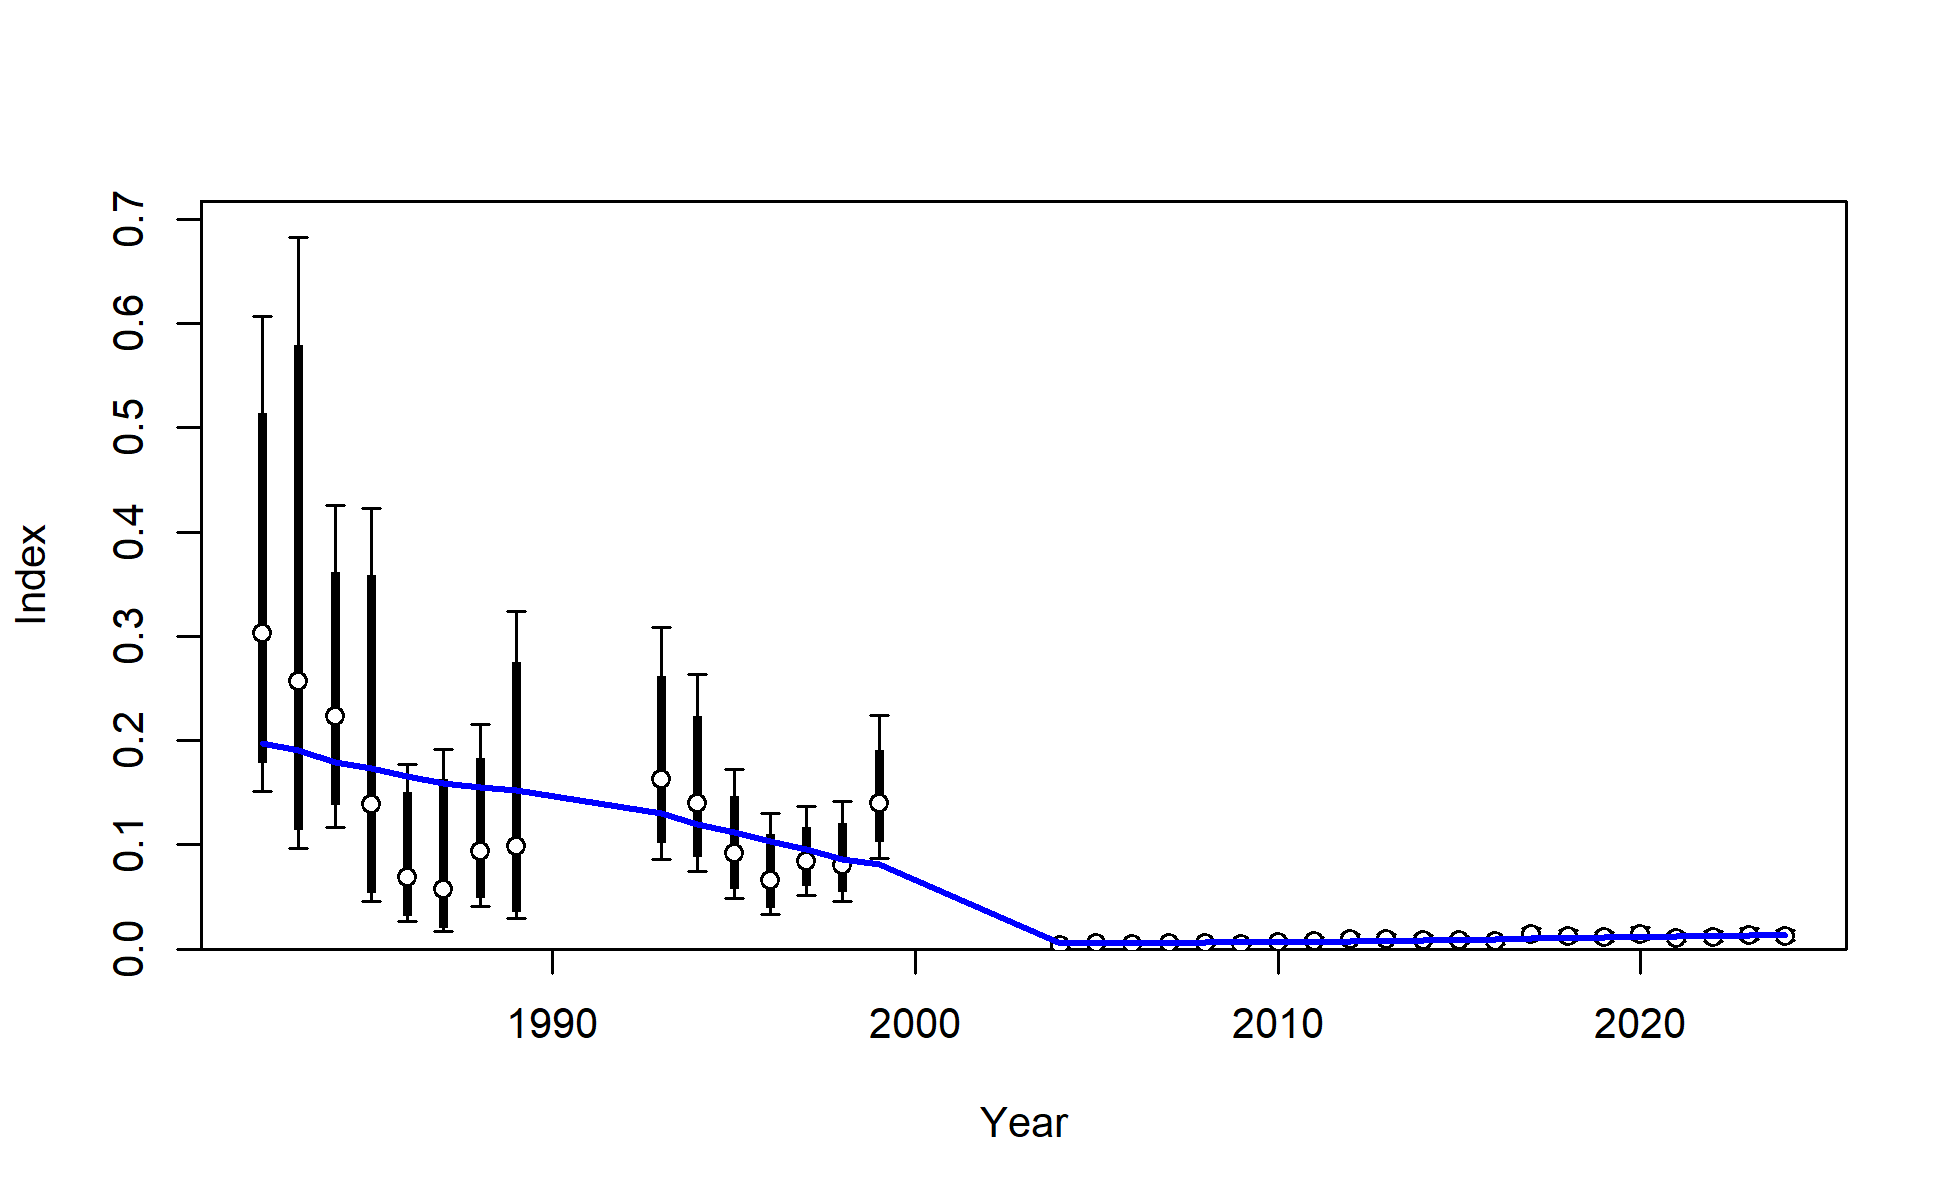
\includegraphics[width=6.5in,height=\textheight,keepaspectratio]{figures/r4ss_plots/plots/index2_cpuefit_6_OR_REC.png}

}

\caption{\label{fig-indexfit6}Fit to the Oregon recreational index.}

\end{figure}%

\begin{figure}

\centering{

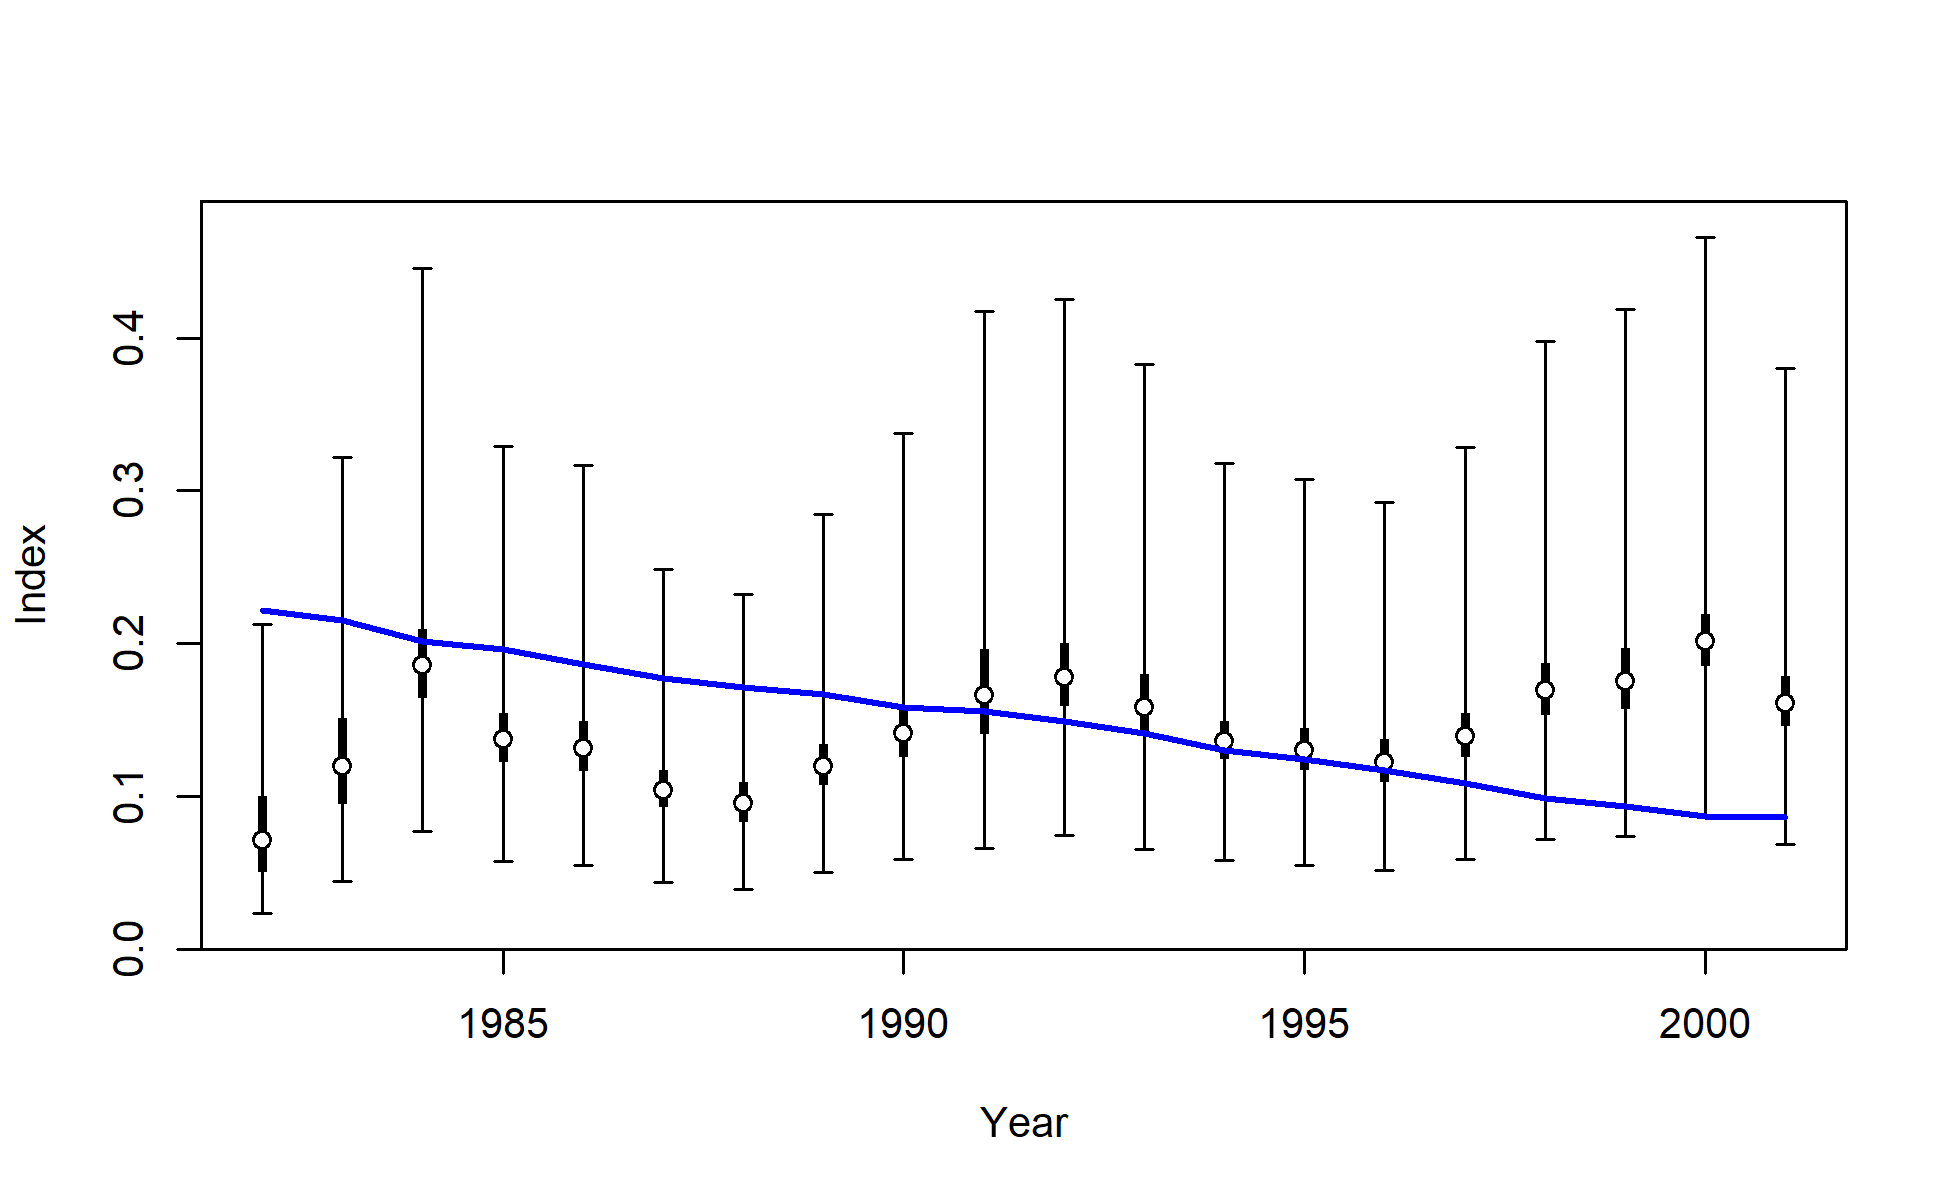
\includegraphics[width=6.5in,height=\textheight,keepaspectratio]{figures/r4ss_plots/plots/index2_cpuefit_7_WA_REC.png}

}

\caption{\label{fig-indexfit7}Fit to the Washington recreational index.}

\end{figure}%

\begin{figure}

\centering{

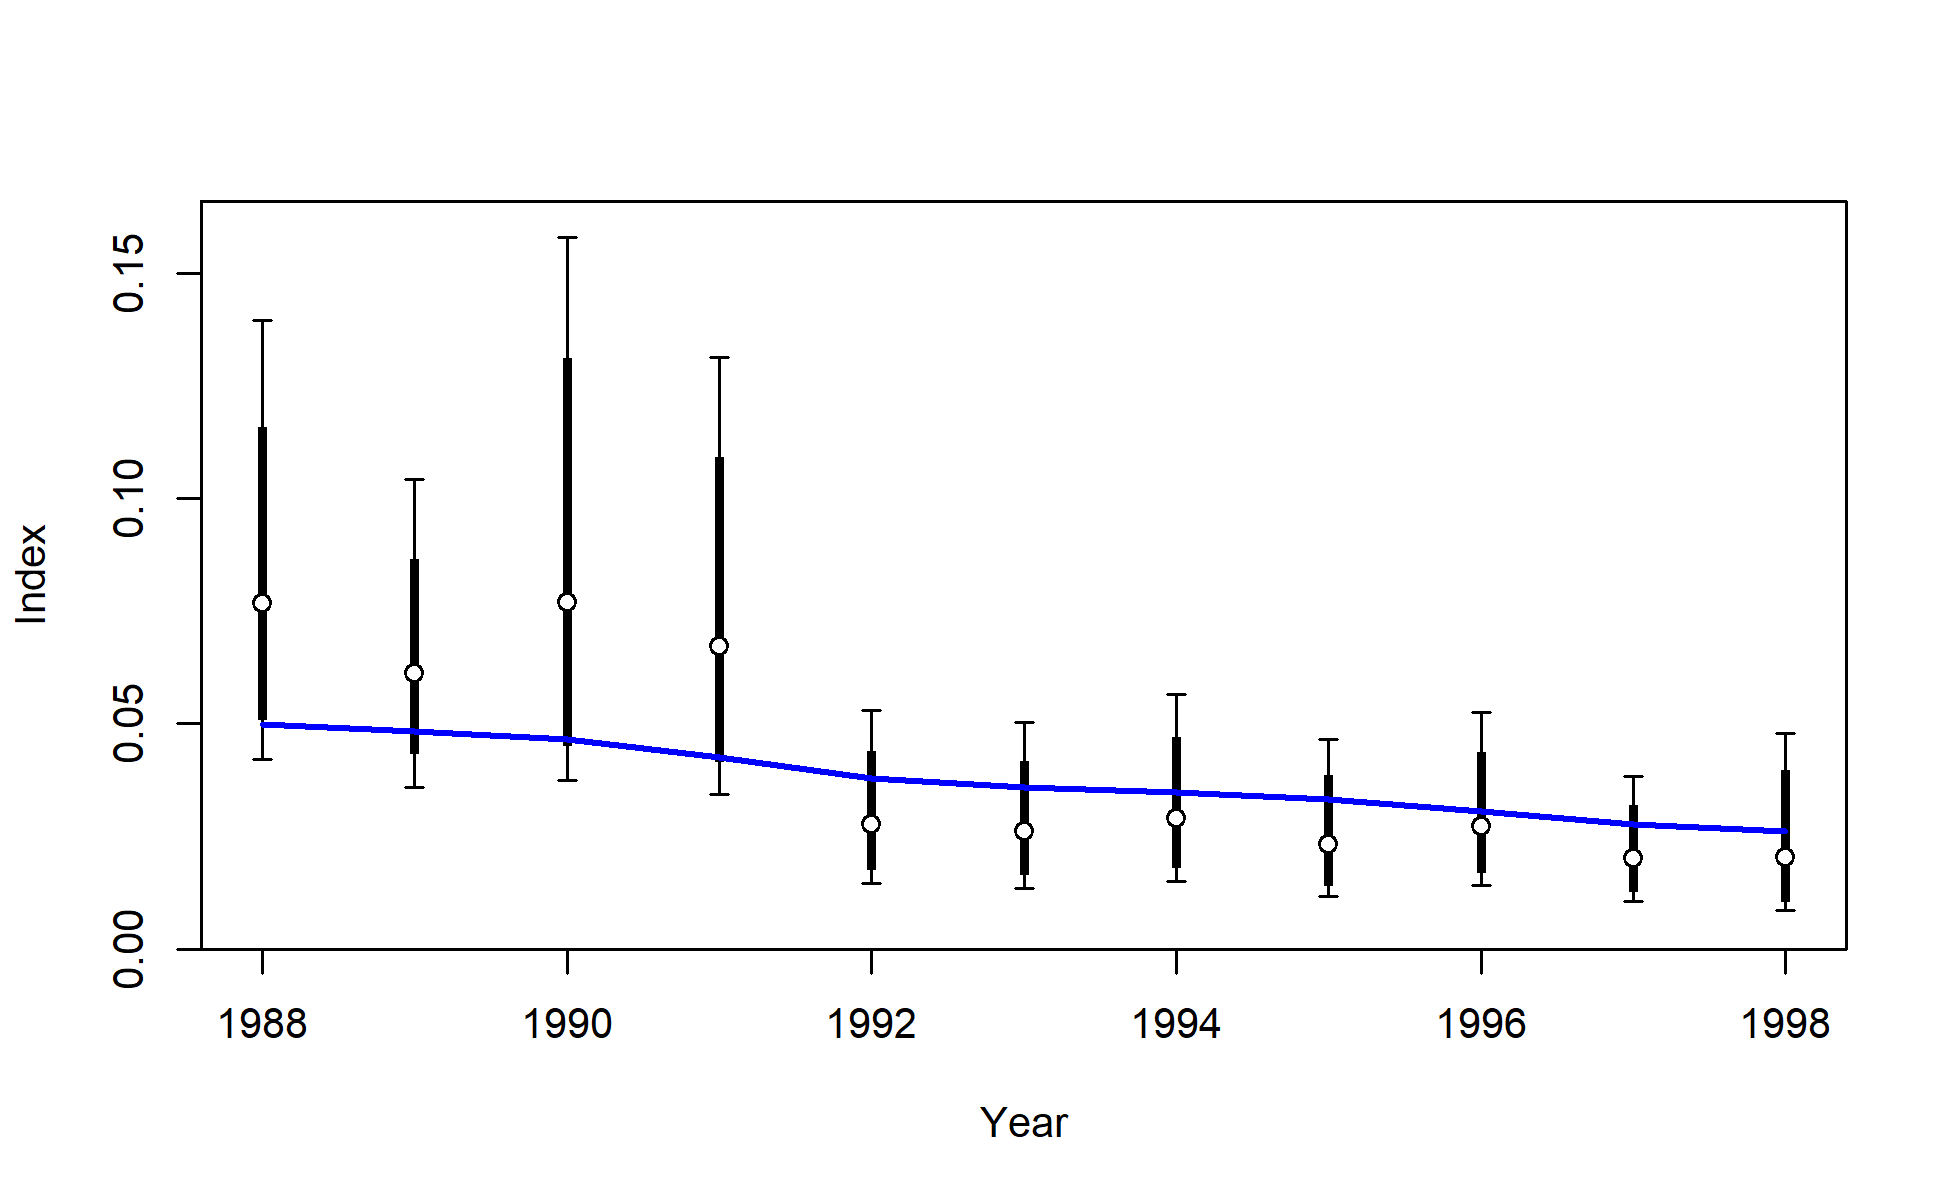
\includegraphics[width=6.5in,height=\textheight,keepaspectratio]{figures/r4ss_plots/plots/index2_cpuefit_8_CACPFV.png}

}

\caption{\label{fig-indexfit8}Fit to the California CPFV observer
index.}

\end{figure}%

\begin{figure}

\centering{

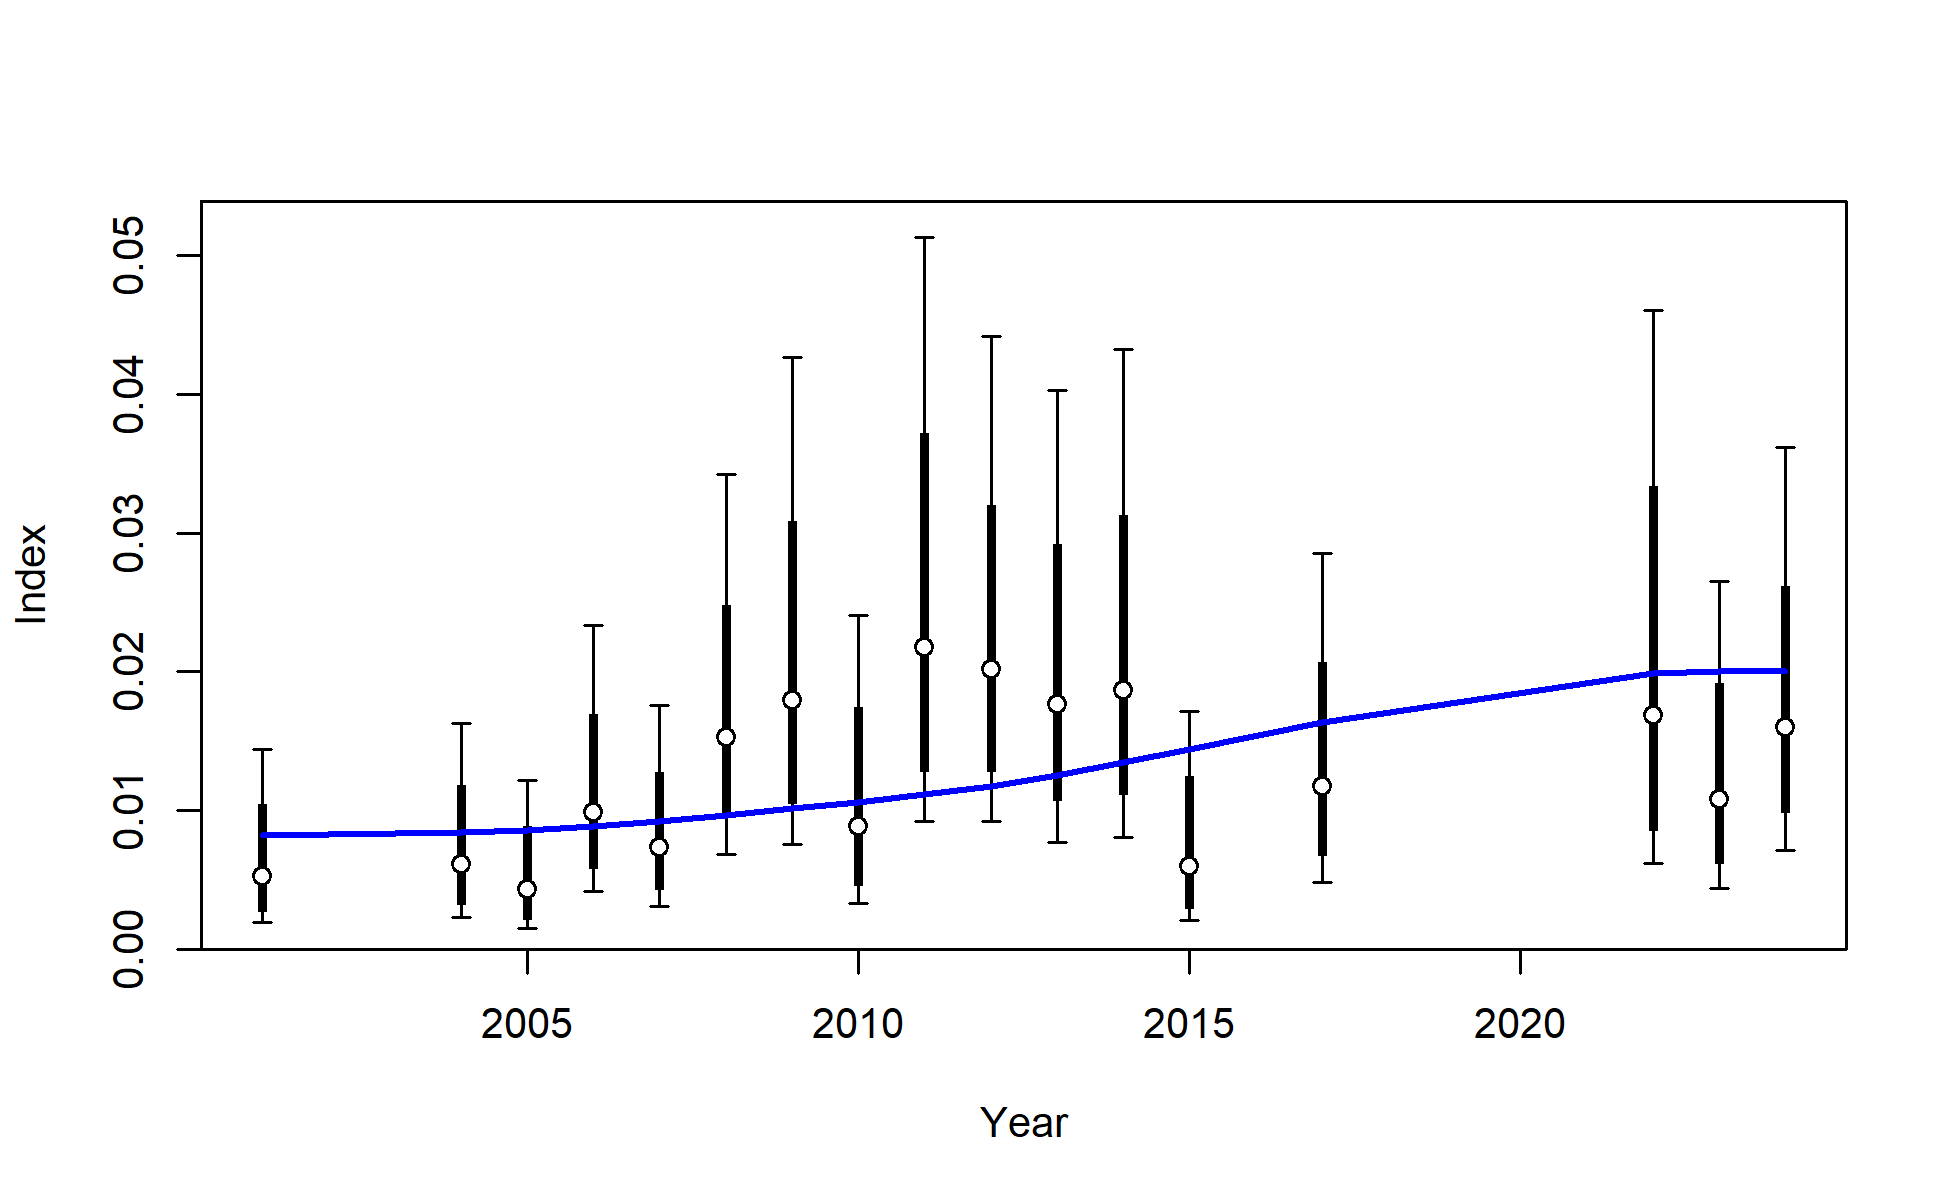
\includegraphics[width=6.5in,height=\textheight,keepaspectratio]{figures/r4ss_plots/plots/index2_cpuefit_9_OR_RECOB.png}

}

\caption{\label{fig-indexfit9}Fit to the Oregon onboard observer (ORFS)
index.}

\end{figure}%

\begin{figure}

\centering{

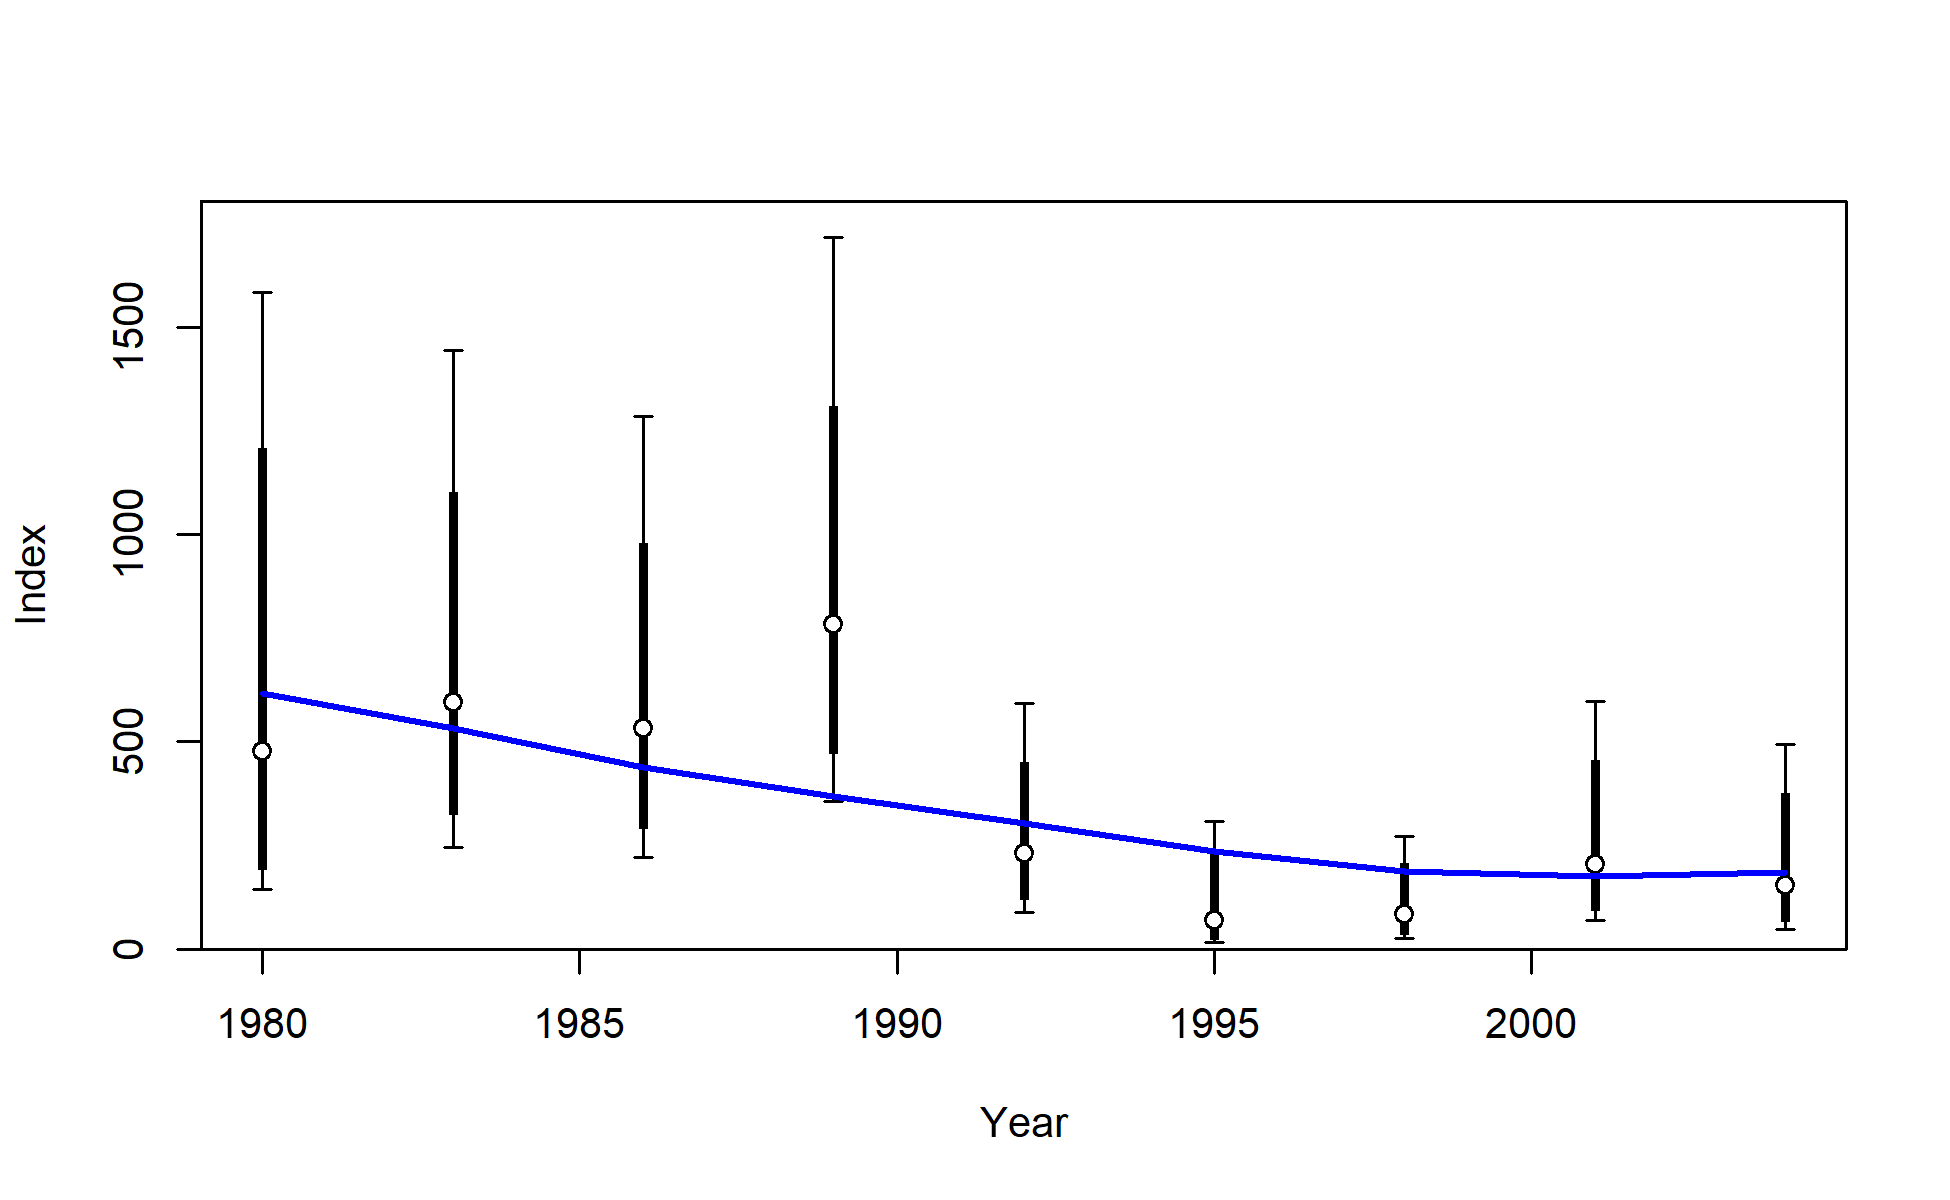
\includegraphics[width=6.5in,height=\textheight,keepaspectratio]{figures/r4ss_plots/plots/index2_cpuefit_10_TRI_ORWA.png}

}

\caption{\label{fig-indexfit10}Fit to the Triennial survey index.}

\end{figure}%

\begin{figure}

\centering{

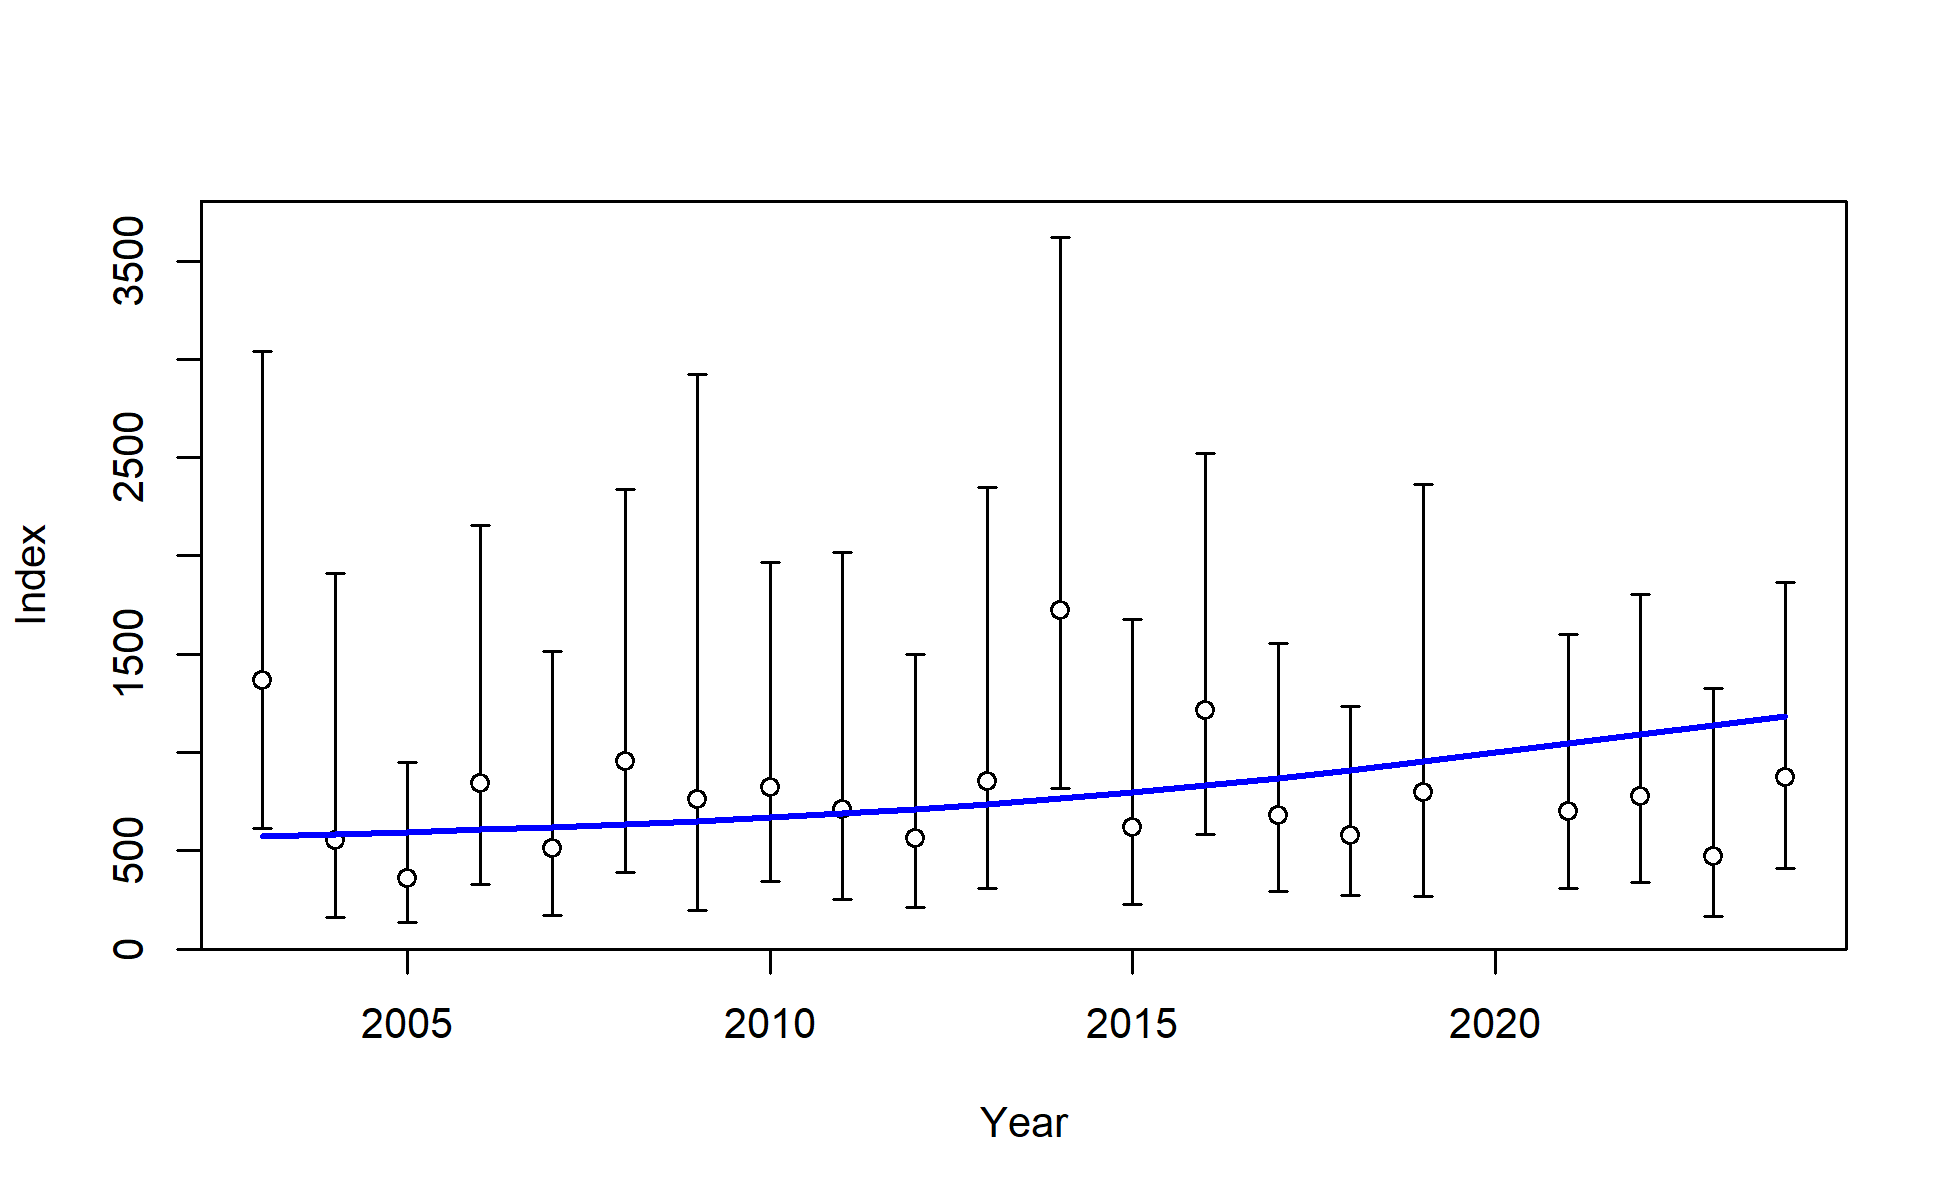
\includegraphics[width=6.5in,height=\textheight,keepaspectratio]{figures/r4ss_plots/plots/index2_cpuefit_11_NWFSC_ORWA.png}

}

\caption{\label{fig-indexfit11}Fit to the WCBTS index.}

\end{figure}%

\begin{figure}

\centering{

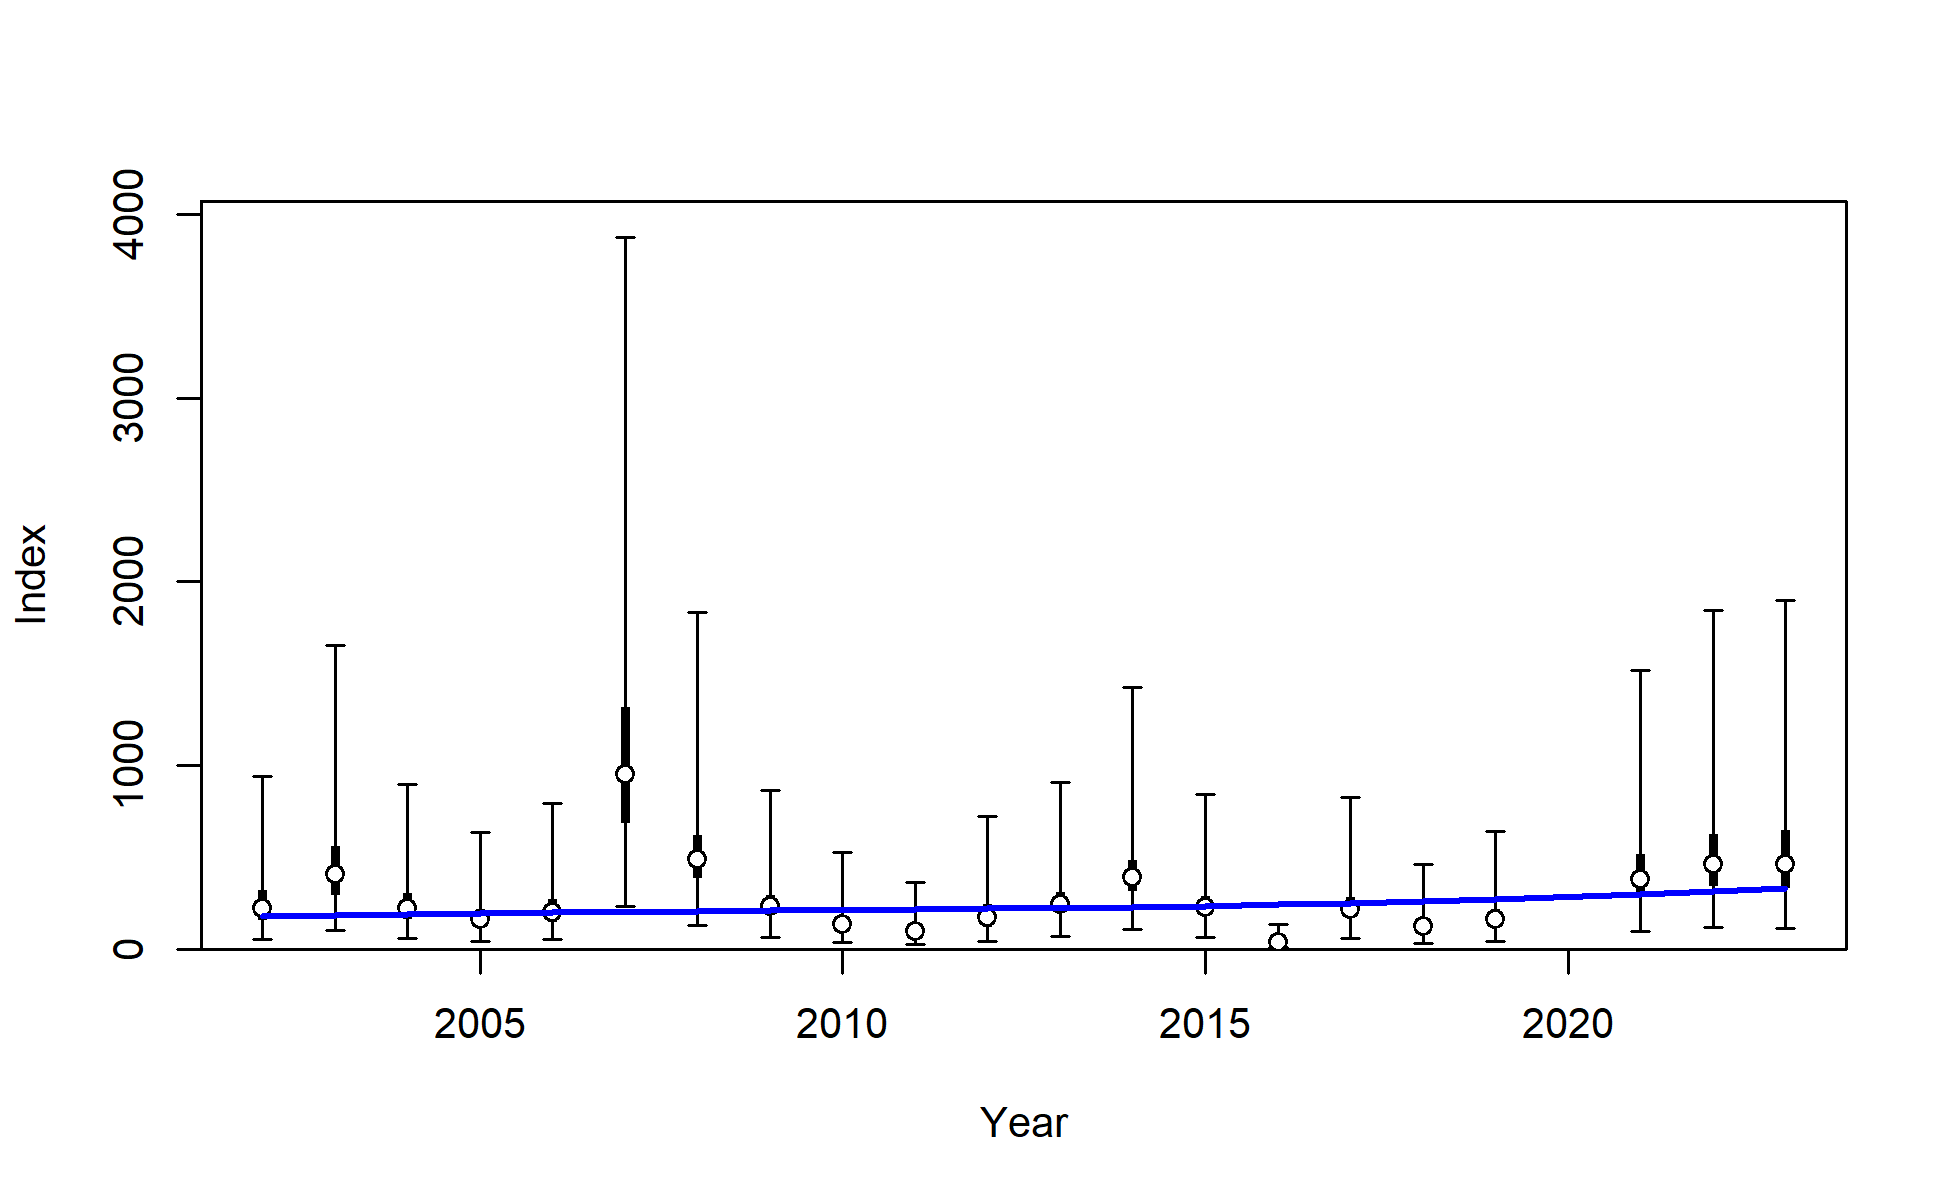
\includegraphics[width=6.5in,height=\textheight,keepaspectratio]{figures/r4ss_plots/plots/index2_cpuefit_12_IPHC_ORWA.png}

}

\caption{\label{fig-indexfit12}Fit to the IPHC survey index.}

\end{figure}%

\clearpage

\begin{figure}

\centering{

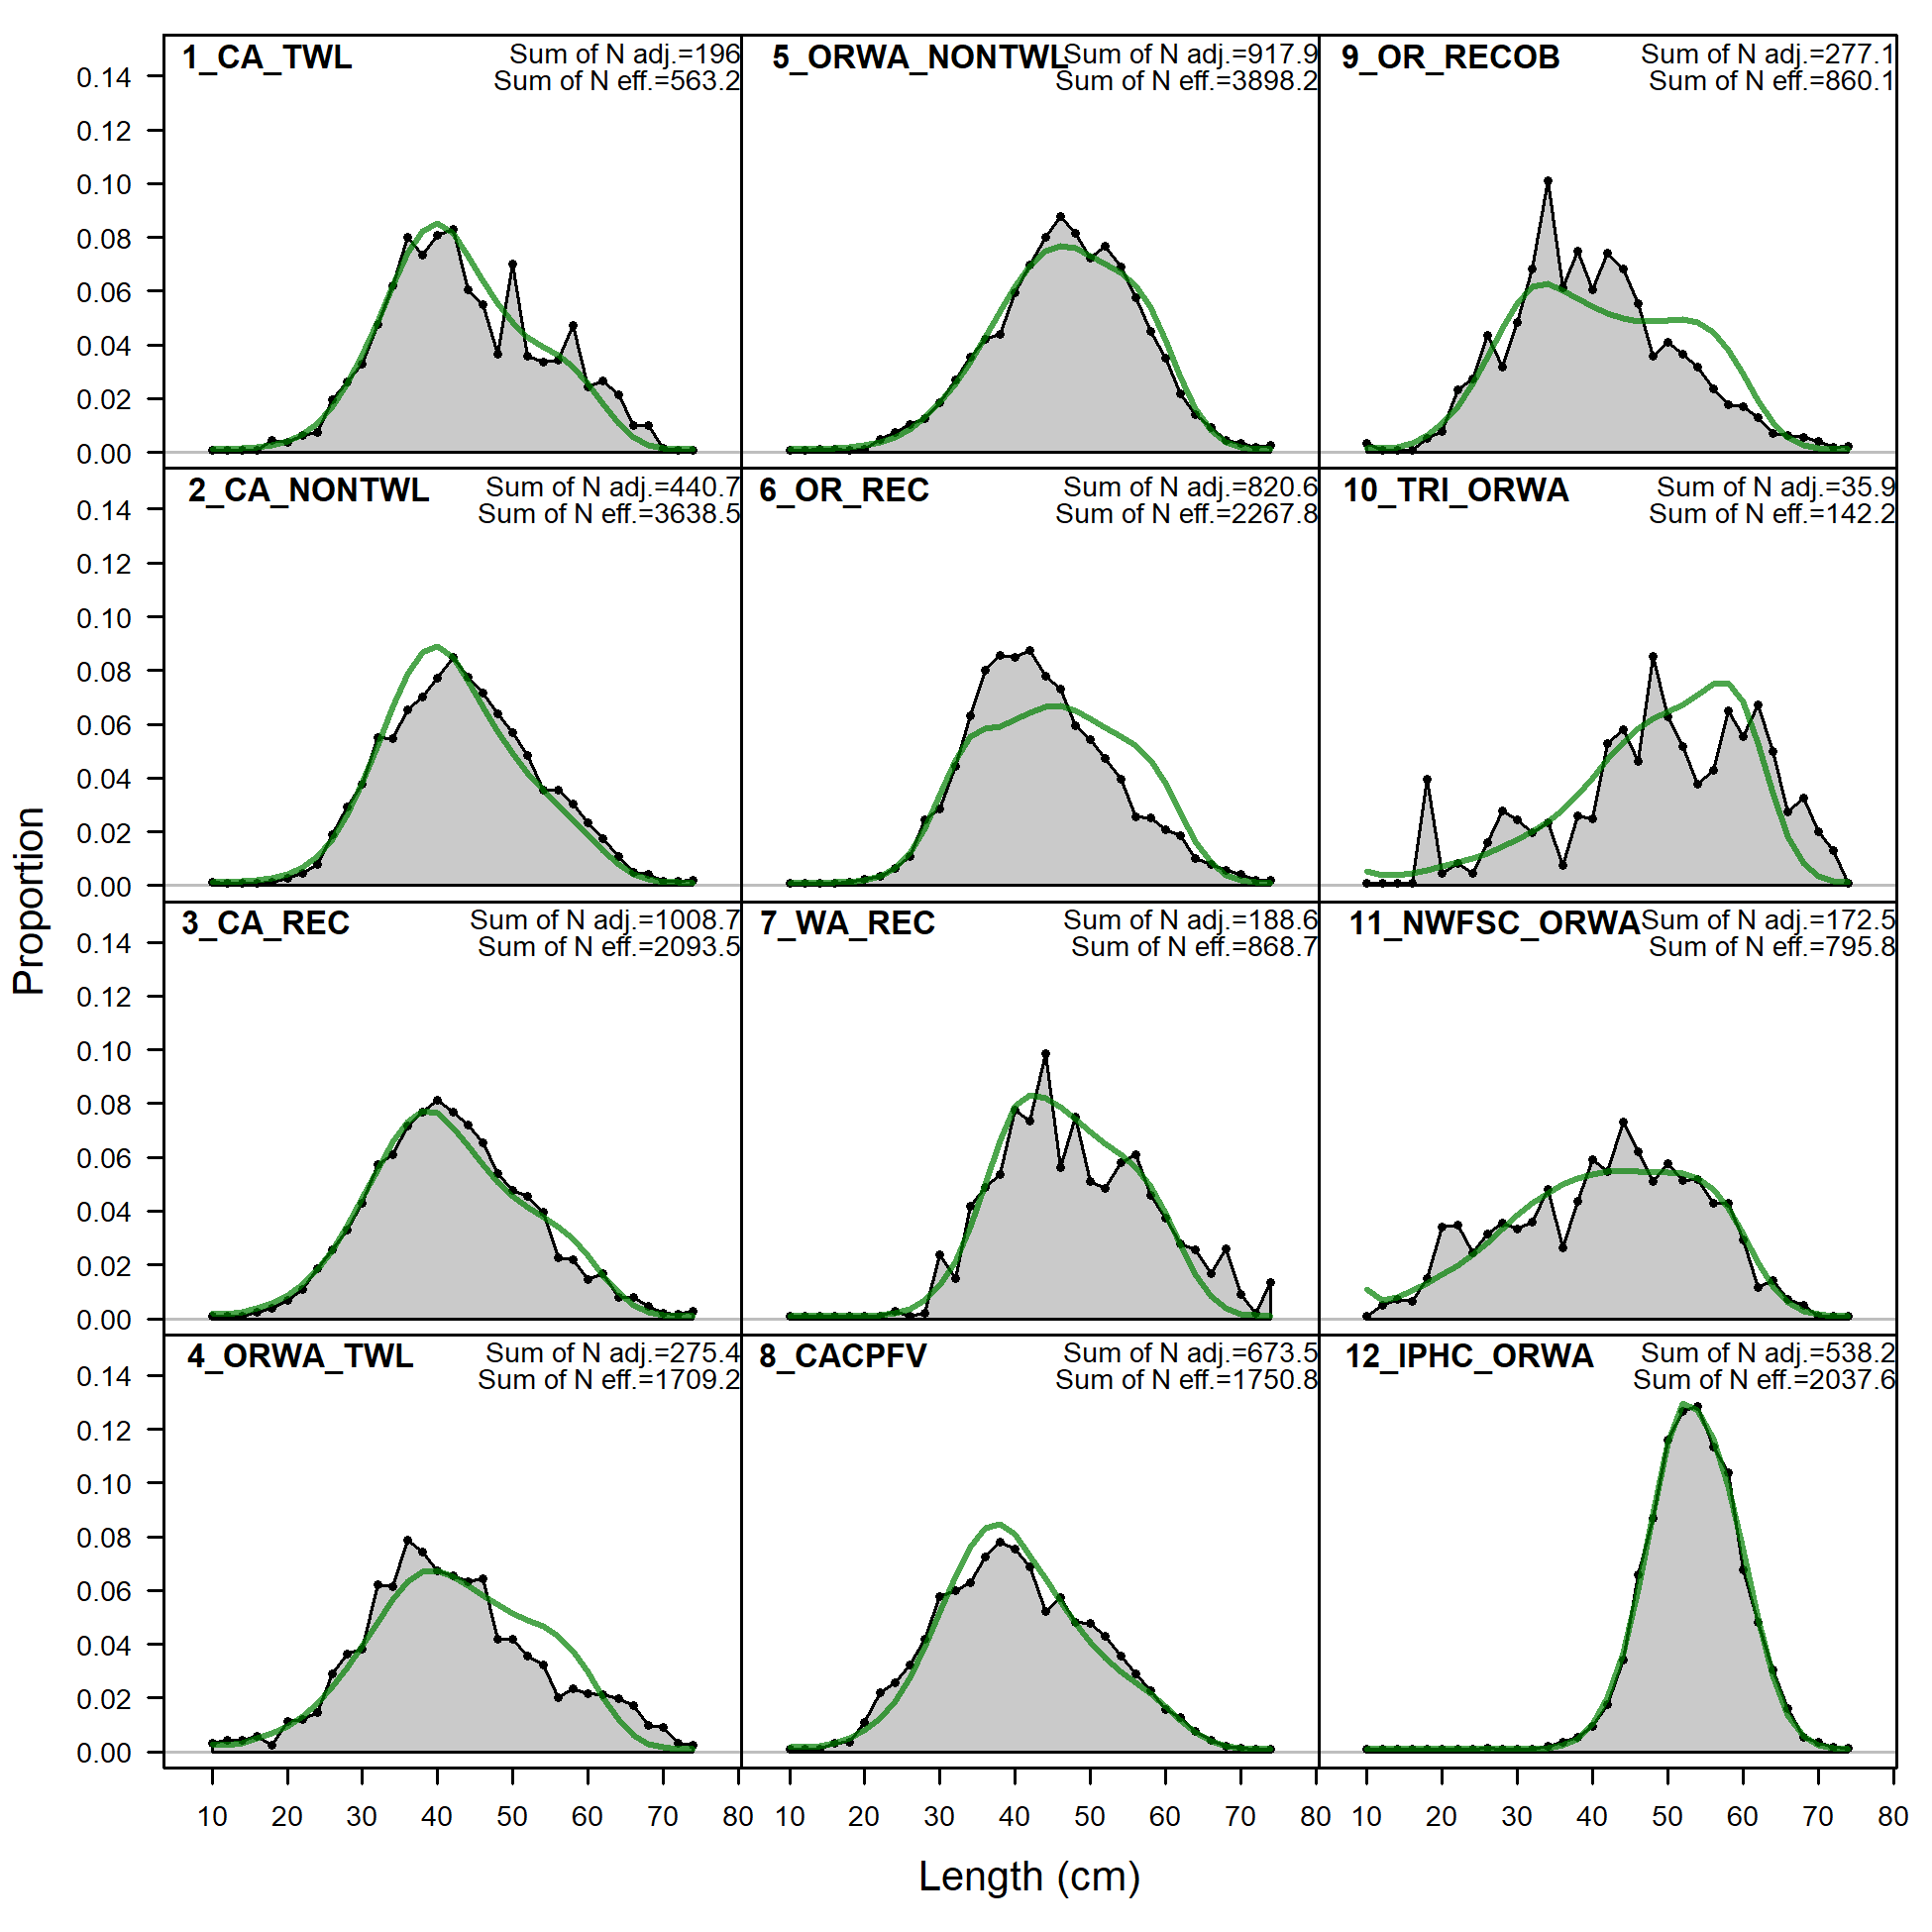
\includegraphics[width=6.5in,height=\textheight,keepaspectratio]{figures/r4ss_plots/plots/comp_lenfit__aggregated_across_time.png}

}

\caption{\label{fig-agglencomps}Fit to length composition data,
aggregated across time by fleet.}

\end{figure}%

\begin{figure}

\centering{

\includegraphics[width=6.5in,height=\textheight,keepaspectratio]{figures/r4ss_plots/plots/comp_lenfit__page1_multi-fleet_comparison.png}

}

\caption{\label{fig-pearsonlenfit1}Pearson residuals, comparing across
fleets, for length composition data (1 of 2). Closed bubbles are
positive residuals (observed \textgreater{} expected) and open bubbles
are negative residuals (observed \textless{} expected).}

\end{figure}%

\begin{figure}

\centering{

\includegraphics[width=6.5in,height=\textheight,keepaspectratio]{figures/r4ss_plots/plots/comp_lenfit__page2_multi-fleet_comparison.png}

}

\caption{\label{fig-pearsonlenfit2}Pearson residuals, comparing across
fleets, for length composition data (2 of 2). Closed bubbles are
positive residuals (observed \textgreater{} expected) and open bubbles
are negative residuals (observed \textless{} expected).}

\end{figure}%

\begin{figure}

\centering{

\includegraphics[width=6.5in,height=\textheight,keepaspectratio]{figures/r4ss_plots/plots/ts7_Spawning_output_with_95_intervals.png}

}

\caption{\label{fig-spout_combined}Estimated spawning output over time
for both areas combined.}

\end{figure}%

\begin{figure}

\centering{

\includegraphics[width=6.5in,height=\textheight,keepaspectratio]{figures/r4ss_plots/plots/ts8_Spawning_output_by_area.png}

}

\caption{\label{fig-spout_area}Estimated spawning output over time and
by area (Area 1 is California, Area 2 is Oregon/Washington combined).}

\end{figure}%

\begin{figure}

\centering{

\includegraphics[width=6.5in,height=\textheight,keepaspectratio]{figures/r4ss_plots/plots/ts2_Total_biomass_(t)_by_area.png}

}

\caption{\label{fig-totalbio}Total biomass (t) over time and by area
(Area 1 is California, Area 2 is Oregon/Washington combined).}

\end{figure}%

\begin{figure}

\centering{

\includegraphics[width=6.5in,height=\textheight,keepaspectratio]{figures/r4ss_plots/plots/ts5_Summary_biomass_(t)_by_area.png}

}

\caption{\label{fig-summbio}Summary biomass (t) over time and by area
(Area 1 is California, Area 2 is Oregon/Washington combined).}

\end{figure}%

\clearpage

\begin{figure}

\centering{

\includegraphics[width=6.5in,height=\textheight,keepaspectratio]{figures/r4ss_plots/plots/ts12_Age-0_recruits_(1000s)_by_area.png}

}

\caption{\label{fig-tsrecuits}Age 0 recruits (1000s) over time and by
area (Area 1 is California, Area 2 is Oregon/Washington combined).}

\end{figure}%

\begin{figure}

\centering{

\includegraphics[width=9in,height=\textheight,keepaspectratio]{figures/diagnostics/2025_base_model_jitter_0.1/jitter.png}

}

\caption{\label{fig-full-jitter}Plot showing 50 jitters with 78\%
returning to the base model likelihood.}

\end{figure}%

\begin{figure}

\centering{

\includegraphics[width=6.5in,height=\textheight,keepaspectratio]{figures/sensitivities/modelingcompare2_spawnbio_uncertainty.png}

}

\caption{\label{fig-sens_model_spout}Spawning output across model
structure sensitivities.}

\end{figure}%

\begin{figure}

\centering{

\includegraphics[width=6.5in,height=\textheight,keepaspectratio]{figures/sensitivities/modelingcompare4_Bratio_uncertainty.png}

}

\caption{\label{fig-sens_model_status}Relative spawning output across
model structure sensitivities.}

\end{figure}%

\begin{figure}

\centering{

\includegraphics[width=6.5in,height=\textheight,keepaspectratio]{figures/sensitivities/comp_datacompare2_spawnbio_uncertainty.png}

}

\caption{\label{fig-sens_data_spout}Spawning output across dataset
inclusion sensitivities.}

\end{figure}%

\begin{figure}

\centering{

\includegraphics[width=6.5in,height=\textheight,keepaspectratio]{figures/sensitivities/comp_datacompare4_Bratio_uncertainty.png}

}

\caption{\label{fig-sens_data_status}Relative spawning output across
dataset inclusion sensitivities.}

\end{figure}%

\begin{figure}

\centering{

\includegraphics[width=6.5in,height=\textheight,keepaspectratio]{figures/sensitivities/indicescompare2_spawnbio_uncertainty.png}

}

\caption{\label{fig-sens_indices_spout}Spawning output across index
inclusion sensitivities.}

\end{figure}%

\begin{figure}

\centering{

\includegraphics[width=6.5in,height=\textheight,keepaspectratio]{figures/sensitivities/indicescompare4_Bratio_uncertainty.png}

}

\caption{\label{fig-sens_indices_status}Relative spawning output across
index inclusion sensitivities.}

\end{figure}%

\clearpage

\begin{figure}

\centering{

\includegraphics[width=6in,height=\textheight,keepaspectratio]{figures/sensitivities/sens_summary.png}

}

\caption{\label{fig-sens_sum}Relative change in management quantities
across models conducted as sensitivities.}

\end{figure}%

\begin{figure}

\centering{

\includegraphics[width=7.6in,height=\textheight,keepaspectratio]{figures/bridging/Timeseries_comp_previous_assessments.png}

}

\caption{\label{fig-status_assmtns}Relative depletion (spawning output)
across Yelloweye Rockfish assessments over time.}

\end{figure}%

\pagebreak

\phantomsection\label{refs}
\begin{CSLReferences}{1}{0}
\bibitem[\citeproctext]{ref-Anderson_2024_SRP}
Anderson, Sean C., Eric J. Ward, Philina A. English, Lewis A. K.
Barnett, and James T. Thorson. 2024. {``sdmTMB: An r Package for Fast,
Flexible, and User-Friendly Generalized Linear Mixed Effects Models with
Spatial and Spatiotemporal Random Fields.''} \emph{bioRxiv},
2022.03.24.485545. \url{https://doi.org/10.1101/2022.03.24.485545}.

\bibitem[\citeproctext]{ref-coombs_1979}
Coombs, C. I. 1979. {``Reef Fishes Near Dipoe Bay, Oregon: Movement and
the Recreational Fishery.''} Master's thesis, Oregon State University.

\bibitem[\citeproctext]{ref-demott_1983}
DeMott, G. E. 1983. {``Movement of Tagged Lingcod and Rockfishes Off
Depoe Bay, Oregon.''} Master's thesis, Oregon State University.

\bibitem[\citeproctext]{ref-drake_status_2010}
Drake J. S., J. M. Cope, E. A. Berntson, and G. D. Williams. 2010.
{``Status Review of Five Rockfish Species in Puget Sound, Washington:
Bocaccio (Sebastes Paucispinis), Canary Rockfish (s. Pinniger),
Yelloweye Rockfish (s. Ruberrimus), Greenstriped Rockfish (s.
Elongatus), and Redstripe Rockfish (s. Proriger).''} NOAA Technical
Memorandum NMFS-NWFSC-108.

\bibitem[\citeproctext]{ref-francis_data_2011}
Francis, R. I. C. Chris. 2011. {``Data Weighting in Statistical
Fisheries Stock Assessment Models.''} \emph{Canadian Journal of
Fisheries and Aquatic Sciences} 68 (6): 1124--38.
\url{https://doi.org/10.1139/f2011-025}.

\bibitem[\citeproctext]{ref-gao_isotope_2010}
Gao, D. L. Dettman, Y., and F. R. Wallace. 2010. {``Isotopic Correlation
(δ18O Versus δ13C) of Otoliths in Identification of Groundfish
Stocks.''} \emph{Transactions of the American Fisheries Society} 139.

\bibitem[\citeproctext]{ref-gertseva_stock_2017}
Gertseva, V. V., and J. M. Cope. 2017. {``Stock Assessment of the
Yelloweye Rockfish (\emph{{Sebastes} Ruberrimus}) in State and {Federal}
Waters Off {California}, {Oregon}, and {Washington}.''} Pacific Fishery
Management Council, 7700 Ambassador Place NE, Suite 200, Portland, OR
97220: Pacific Fishery Management Council.

\bibitem[\citeproctext]{ref-hannah_movement_2011}
Hannah, R. W., and P. S. Rankin. 2011. {``Site Fidelity and Movement of
Eight Species of Pacific Rockfish at a High-Relief Rocky Reef on the
Oregon Coast.''} \emph{North American Journal of Fisheries Management}
31: 483--94. \url{https://doi.org/10.1080/02755947.2011.591239}.

\bibitem[\citeproctext]{ref-hart_pacific_1973}
Hart, J. L. 1973. {``Pacific Fishes of {C}anada.''} 180. St. Andrews,
NB, Canada: Fisheries Research Board of Canada Bulletin.

\bibitem[\citeproctext]{ref-Johnson_indexwc}
Johnson, Kelli F., Sean C. Anderson, Chantel R. Wetzel, Eric J. Ward,
and Ian G. Taylor. 2025. \emph{Indexwc: Run Indices for West Coast
Groundfish Assessments}.
\url{https://github.com/pfmc-assessments/indexwc}.

\bibitem[\citeproctext]{ref-keller2017northwest}
Keller, A. A, J. R. Wallace, and R. D. Methot. 2017. {``The Northwest
Fisheries Science Center's West Coast Groundfish Bottom Trawl Survey:
History, Design, and Description.''} \emph{U.S. Department of Commerce,
NOAA Technical Memorandum NMFS-NWFSC-136}.
\url{https://doi.org/10.7289/V5/TM-NWFSC-136}.

\bibitem[\citeproctext]{ref-kristensen_tmb:_2016}
Kristensen, Kasper, A. Nielsen, Casper W Berg, H. J. Skaug, and B. M.
Bell. 2016. {``{TMB}: {Automatic} {Differentiation} and {Laplace}
{Approximation}.''} \emph{Journal of Statistical Software} 70: 1--21.

\bibitem[\citeproctext]{ref-love_rockfishes_2002}
Love, M. S., M. Yoklavich, and L. Thorsteinson. 2002. \emph{The
{Rockfishes} of the {Northeast} {Pacific}}. 1st Edition. Berkeley:
University of California Press.

\bibitem[\citeproctext]{ref-monk_documentation_2013}
Monk, E. J. Dick, M., and D. Pearson. 2013. {``Documentation of a
Relational Database for the Oregon Sport Groundfish Onboard Sampling
Program.''} NOAA Technical Memorandum NOAA -TM-NMFS-SWFSC-519.

\bibitem[\citeproctext]{ref-rasmuson_movement_2025}
Rasmuson LK, Lawrence KA, Blume MTO, and Chapple TK. 2025. {``Routine
Large-Scale Movements of the Yelloweye Rockfish (Sebastes
Ruberrimus).''} \emph{Frontiers in Marine Science} 12.
\url{https://doi.org/10.3389/fmars.2025.1539206}.

\bibitem[\citeproctext]{ref-siegle_genetics_2013}
Siegle, Taylor, M. R., and K. L. Yamanaka. 2013. {``Subtle Population
Genetic Structure in Yelloweye Rockfish (Sebastes Ruberrimus) Is
Consistent with a Major Oceanographic Division in British Columbia,
Canada.''} \emph{PloS One} 8. \url{https://doi.org/p.e71083}.

\bibitem[\citeproctext]{ref-stewart_bootstrapping_2014}
Stewart, Ian J., and Owen S. Hamel. 2014. {``Bootstrapping of Sample
Sizes for Length- or Age-Composition Data Used in Stock Assessments.''}
\emph{Canadian Journal of Fisheries and Aquatic Sciences} 71 (4):
581--88. \url{https://doi.org/10.1139/cjfas-2013-0289}.

\bibitem[\citeproctext]{ref-thorson_geostatistical_2015}
Thorson, J. T., A. O. Shelton, E. J. Ward, and H. J. Skaug. 2015.
{``Geostatistical Delta-Generalized Linear Mixed Models Improve
Precision for Estimated Abundance Indices for {West} {Coast}
Groundfishes.''} \emph{ICES Journal of Marine Science} 72 (5):
1297--1310. \url{https://doi.org/10.1093/icesjms/fsu243}.

\bibitem[\citeproctext]{ref-Whitman_2024}
Whitman, Alison D. 2024. {``Oregon Historical Marine Recreational Catch
Reconstruction (1979-2000).''} ODFW Science Bulletin 2024-09.

\end{CSLReferences}




\end{document}
